\documentclass[thesis]{thesis-gwu}[2018/05/21]

\newcommand{\SO}[1]{\ensuremath{\mathrm{SO}(#1)}}
\newcommand{\SE}[1]{\ensuremath{\mathrm{SE}(#1)}}
\renewcommand{\so}[1]{\ensuremath{\mathfrak{so}(#1)}}
\newcommand{\Sph}{\ensuremath{\mathbb{S}}}
\newcommand{\norm}[1]{\ensuremath{\left\| #1 \right\|}}
\newcommand{\tr}[1]{\ensuremath{\mathrm{tr}\left( #1 \right)}}
\newcommand{\etr}[1]{\ensuremath{\mathrm{etr}\left( #1 \right)}}
\newcommand{\expect}[1]{\ensuremath{\mathrm{E}\left[ #1 \right]}}
\newcommand{\expectbar}[1]{\ensuremath{\bar{\mathrm{E}}\left[ #1 \right]}}
\newcommand{\cov}[2]{\ensuremath{\mathrm{cov}\left( #1, #2 \right)}}
\newcommand{\covbar}[2]{\ensuremath{\overline{\mathrm{cov}}\left( #1, #2 \right)}}
\newcommand{\expb}[1]{\ensuremath{\exp\left\{ #1 \right\}}}
\newcommand{\diff}{\ensuremath{\mathrm{d}}}
\newcommand{\diag}{\ensuremath{\mathrm{diag}}}

\newtheorem{definition}{Definition}[chapter]
\newtheorem{theorem}{Theorem}[chapter]
\newtheorem{lemma}{Lemma}[chapter]
\newtheorem{corollary}{Corollary}[chapter]

\DeclareMathAlphabet{\mathcal}{OMS}{cmsy}{m}{n}

\makeatletter
\newcommand\approxsim{\mathpalette\@approxsim\relax}
\newcommand\@approxsim[2]{%
	\mathrel{%
		\ooalign{%
			$\m@th#1\sim$\cr
			\hidewidth$\m@th#1:$\hidewidth\cr
		}%
	}%
}
\makeatother

% this package is only used to generate some random text. 
% it is not needed in a true document
\usepackage{lipsum}

% !TEX root = ../thesis-WW.tex

% --------- FRONT MATTER PAGES ---------------------
% Title of the thesis
\title{Geometric Formulation of Uncertainties and Estimation \\ for Three-Dimensional Rotations}

% Author name
\author{Weixin Wang}

% Previous degrees
\bsdepartment{Mechanical Engineering}
\bsschool{Tsinghua University}
\bsgrad{May 2016}

\msdepartment{Mechanical Engineering}
\msschool{University of Wisconsin-Madison}
\msgrad{December 2018}
\showmsdegree % you can show or hide the MS degree line 
% \hidemsdegree

% PhD degree commands
% Committee
\showcommitteepage % hide this page if you're doing a MS thesis
%\hidecommitteepage 
\committee{ %
Dr. Taeyoung Lee, Professor of Mechanical and Aerospace Engineering,\\ 
George Washington University, Dissertation Director\\ % remember to add a space between committee members

Dr. Kausik Sarkar, Professor of Mechanical and Aerospace Engineering, \\
George Washington University, Committee Chair\\

Dr. Peng Wei, Assistant Professor of Mechanical and Aerospace Engineering, \\
George Washington University, Committee Member\\

Dr. Chung Hyuk Park, Associate Professor of Biomedical Engineering, \\
George Washington University, Committee Member\\

Dr. Kyle DeMars, Associate Professor of Aerospace Engineering, \\
Texas A\&M University, Committee Member\\
}

% Chair must be entered separately for formatting reasons.
\chair{Taeyoung Lee}
\chairtitle{Professor of Mechanical and Aerospace Engineering}

% Uncomment the following lines if there are two dissertation co-directors.
%\hascochair
%\cochair{Murray Snyder}
%\cochairtitle{Professor of Mechanical and Aerospace Engineering}

% Department
\department{Mechanical and Aerospace Engineering}

\phdgrad{July 21, 2022}
\defensedate{July 21, 2022}
% Year of completion for copyright page and perhaps other places
\year=2022

% Copyright page
%\copyrightholder{Someone else}

% Dedication
%\dedication{ %
%Include a fancy quote or dedication
%}

% Acknowledgments
\acknowledgments{
    Here you can acknowledge all of those people who have helped you to reach this point.
    It's rare that any work is done in a vacuum and your research is no exception.
    Feel free to be grateful for all those who've aided you along your way.
}

% -----------------------------------------------------------------
% Typically only one of Preface/Foreward/Prologue would be in your thesis.
% To choose one simply delete the others and they will automatically dissappear

% Preface
\preface{
    This is the preface. 
    It's another front matter page that offers additional detail into your work.
    Typically, only one (preface OR prologue OR foreword) is used. 
    You can remove the other sections by deleting them inside \texttt{tex/frontmatter.tex} or using the appropriate show or hide commands.
}

\prologue{
    This is the prologe. 
    It's another front matter page that offers additional detail into your work.
    Typically, only one (preface OR prologue OR foreword) is used. 
    You can remove the other sections by deleting them inside \texttt{tex/frontmatter.tex} or using the appropriate show or hide commands.
}

\foreword[2]{
    This is the forword. 
    It's another front matter page that offers additional detail into your work.
    Typically, only one (preface OR prologue OR foreword) is used. 
    You can remove the other sections by deleting them inside \texttt{tex/frontmatter.tex} or using the appropriate show or hide commands.
}
% ----------------------------------------------------------------------

% commands to show or hide front matter pages

\showcopyright
\showabstract
\showcommitteepage
\hidededication
\showacknowledgments
\hidepreface
\hideprologue
\hideforeword

% ------------ TABLE OF CONTENTS ----------------------
% Commands to hide or show lists of figures, tables, etc.
\showlistoffigures
\showlistoftables
\hidenomenclature

% --------- ACRONYMS and SYMBOLS ------------------------------
% TODO Deprecate the entire acronym package and switch to glossaries

% You can either use the acronymn or glossaries package (both work)
% Definition of any abbreviations used.
\abbreviations{
    \acro{CRTBP}{Circular Restricted Three Body Problem}
    \acro{NSA}{National Security Agency}
    \acro{SSME}{Space Shuttle Main Engine}
}
% call an abbreviation using \ac{abbrev}

% symbols and acronyms only show up when used in the text
\symbols{
    \acro{J}{Moment of Inertia}
}       

% if you want acronymn (simpler) then change these to show
\hidelistofabbreviations
\hidelistofsymbols

% if you want glossaries (more powerful) then leave above as hide
% GLOSSARIES package options - automatically turns off front pages from acronym package

% acronymns and symbols are basically the same, but there are two provided 
% locations where they can show up
\setabbreviationstyle[acronym]{long-short}
\setabbreviationstyle[abbreviation]{long-short}
\makeglossaries
% you can hide/show the glossaries page
\showglossarieslistofabbreviations
\showglossarieslistofsymbols
\showglossariesglossaryofterms

% acronyms defined in glossaries
% defining abbreviations like this allows for autocompletion
\newglossaryentry{IMU}{
    name={IMU},
    type=\glsxtrabbrvtype,
    description={Inertial Measurement Unit}
}

\newglossaryentry{GNSS}{
	name={GNSS},
	type=\glsxtrabbrvtype,
	description={Global Navigation Satellite System}
}

\newglossaryentry{MFG}{
	name={MFG},
	type=\glsxtrabbrvtype,
	description={Matrix Fisher--Gaussian Distribution}
}

\newglossaryentry{EKF}{
	name={EKF},
	type=\glsxtrabbrvtype,
	description={Extended Kalman Filter}
}

\newglossaryentry{MEKF}{
	name={MEKF},
	type=\glsxtrabbrvtype,
	description={Multiplicative Extended Kalman Filter}
}

\newglossaryentry{UKF}{
	name={UKF},
	type=\glsxtrabbrvtype,
	description={Unscented Kalman Filter}
}

\newglossaryentry{SLAM}{
	name={SLAM},
	type=\glsxtrabbrvtype,
	description={Simultaneous Localization and Mapping}
}

\newglossaryentry{IEKF}{
	name={IEKF},
	type=\glsxtrabbrvtype,
	description={Invariant Extended Kalman Filter}
}

\newglossaryentry{MSCKF}{
	name={MSCKF},
	type=\glsxtrabbrvtype,
	description={Multi-State Constraint Kalman Filter}
}

\newglossaryentry{BCH}{
	name={BCH},
	type=\glsxtrabbrvtype,
	description={Baker--Campbell--Hausdorff Formula}
}

\newglossaryentry{psvd}{
	name={pSVD},
	type=\glsxtrabbrvtype,
	description={proper Singular Value Decomposition}
}

\newglossaryentry{MLE}{
	name={MLE},
	type=\glsxtrabbrvtype,
	description={Maximum Likelihood Estimation}
}

\newglossaryentry{BG}{
	name={BG},
	type=\glsxtrabbrvtype,
	description={Bingham--Gaussian Distribution}
}

\newglossaryentry{MMSE}{
	name={MMSE},
	type=\glsxtrabbrvtype,
	description={Minimum Mean Square Estimate}
}


% glossary entries
\newglossaryentry{stiefel}{
    name=Stiefel manifold,
    description={An orthogonal $r$ frame in $\mathbb{R}^n$ with $r\leq n$.}
}

\newglossaryentry{normalizing}{
	name=normalizing constant,
	description={A constant for an un-normalized probability density function such that it integrates into one.}
}

\newglossaryentry{moment}{
	name=moment,
	description={The expectation of a random variable.}
}

\newglossaryentry{Haar}{
	name=Haar measure,
	description={The bi-invariant measure on $\SO{3}$ for integration of functions on $\SO{3}$. In is normalized such that $\SO{3}$ has unit volume.}
}

\newglossaryentry{inertial}{
	name=inertial frame,
	description={The reference frame that is assumed to be fixed in a navigation problem.}
}

\newglossaryentry{body-fixed}{
	name=body-fixed frame,
	description={The reference frame fixed to a rigid body.}
}

\newglossaryentry{recursive Bayesian filter}{
	name=recursive Bayesian filter,
	description={A stochastic estimator that estimates the state of a dynamical system by calculating the posterior distribution conditioned on the history of all measurements.}
}

\newglossaryentry{uncertainty propagation}{
	name=uncertainty propagation,
	description={Calculate how the probability density function of the state of a dynamical system evolves in time.}
}

\newglossaryentry{measurement update}{
	name=measurement update,
	description={Calculate the posterior density function from the prior and likelihood, using the Bayes' formula.}
}

\newglossaryentry{mle}{
	name=maximum likelihood estimation,
	description={Inference of the parameters of a probability distribution by maximizing the likelihood function of measurements.}
}

\newglossaryentry{kl}{
	name=KL-divergence,
	description={A metric indicating the difference between two probability distributions.}
}

\newglossaryentry{lm}{
	name=LM algorithm,
	description={An iterative gradient based algorithm to solve nonlinear minimum least square problems.}
}

% symbols
\newglossaryentry{SEN}{
	type=symbols,
	name={$\SE{n}$},
	sort=SEN,
	description={The $n$-dimensional special Euclidean group.}
}

\newglossaryentry{SON}{
    type=symbols,
    name={$\SO{n}$},
    sort=SON,
    description={The $n$-dimensional special orthogonal group.}
}

\newglossaryentry{SUN}{
	type=symbols,
	name={$\mathrm{SU}(n)$},
	sort=SUN,
	description={The $n$-dimensional special unitary group.}
}

\newglossaryentry{soN}{
	type=symbols,
	name={$\so{n}$},
	sort=soN,
	description={The Lie algebra of $\SO{n}$.}
}

\newglossaryentry{real}{
	type=symbols,
	name={$\mathbb{R}^n$},
	sort=R,
	description={The $n$-dimensional Euclidean space.}
}

\newglossaryentry{sph}{
	type=symbols,
	name={$\Sph^n$},
	sort=sph,
	description={Unit $n$-sphere.}
}

\newglossaryentry{int}{
	type=symbols,
	name={$\mathbb{Z}$},
	sort=z,
	description={The space of integers.}
}

\newglossaryentry{gamma}{
	type=symbols,
	name={$\Gamma(x)$},
	sort=gamma,
	description={Gamma function.}
}

\newglossaryentry{bessel}{
	type=symbols,
	name={$I_{\nu}(x)$},
	sort=Iv,
	description={Modified Bessel function of the first kind with order $\nu$.}
}

\newglossaryentry{hat}{
	type=symbols,
	name={$\hat{x}$},
	sort=hat,
	description={The hat map that identifies $\mathbb{R}^3$ to $\so{3}$.}
}

\newglossaryentry{vee}{
	type=symbols,
	name={$x^\vee$},
	sort=hat2,
	description={The vee map, inverse of the hat map.}
}

\newglossaryentry{exp}{
	type=symbols,
	name={$\exp(x)$},
	sort=exp,
	description={The exponential of a number $x\in\mathbb{R}$, or the exponential map of $x\in\so{3}$.}
}

\newglossaryentry{bracket}{
	type=symbols,
	name={$[A,B]$},
	sort=bracket,
	description={The Lie bracket for $A,B\in\so{3}$.}
}

\newglossaryentry{mf}{
	type=symbols,
	name={$\mathcal{M}(F)$},
	sort=matrixFisher,
	description={The matrix Fisher distribution with parameter $F$.}
}

\newglossaryentry{diag}{
	type=symbols,
	name={$\diag(x_1,\ldots,x_n)$},
	sort=diag,
	description={The (block) diagonal matrix with the diagonal terms given by $x_1,\ldots,x_n$.}
}

\newglossaryentry{vec}{
	type=symbols,
	name={$\mathrm{vec}(A)$},
	sort=vec,
	description={Concatenation of the columns of matrix $A$ into a column vector.}
}

\newglossaryentry{kron}{
	type=symbols,
	name={$\otimes$},
	sort=otime,
	description={Quaternion multiplication or Kronecker product depending on the context.}
}

\newglossaryentry{normal}{
	type=symbols,
	name={$\mathcal{N}(\mu,\Sigma)$},
	sort=normal,
	description={Normal distribution with mean $\mu$, and covariance matrix $\Sigma$.}
}

\newglossaryentry{von}{
	type=symbols,
	name={$\mathcal{VM}(\mu,\kappa)$},
	sort=von,
	description={The von Mises (Fisher) distribution with mean direction $\mu$, and concentration parameter $\kappa$.}
}

\newglossaryentry{MFGs}{
	type=symbols,
	name={$\mathcal{MG}(\mu,\allowbreak \Sigma,\allowbreak P,\allowbreak U,\allowbreak S,\allowbreak V)$},
	sort=MFG,
	description={The matrix Fisher--Gaussian distribution with parameters $(\mu,\Sigma,P,U,S,V)$.}
}

\newglossaryentry{bingham}{
	type=symbols,
	name={$\mathcal{B}(A)$},
	sort=bingham,
	description={The Bingham distribution with parameter $A$.}
}

\newglossaryentry{BGs}{
	type=symbols,
	name={$\mathcal{BG}(\mu,\Sigma,P,M,Z)$},
	sort=BG,
	description={The Bingham--Gaussian distribution with parameters $(\mu,\Sigma,P,M,Z)$.}
}

\newglossaryentry{phi}{
	type=symbols,
	name={$\varphi$},
	sort=phi,
	description={The homomorphism from $\Sph^3$ to $\SO{3}$.}
}

\newglossaryentry{trace}{
	type=symbols,
	name={$\tr{A}$},
	sort=trace,
	description={The trace of matrix $A$.}
}

\newglossaryentry{etr}{
	type=symbols,
	name={$\etr{A}$},
	sort=etr,
	description={An abbreviation of $\exp(\tr{A})$.}
}

\newglossaryentry{comb}{
	type=symbols,
	name={$\mathcal{C}(n,k)$},
	sort=comb,
	description={The set of all $k$-partitions of the set $\{1,2,\ldots,n\}$. For example $\mathcal{C}(3,2) = \Big\{ \big\{\{1\}, \allowbreak \{2,3\}\big\}, \allowbreak \big\{\{2\}, \allowbreak \{1,3\}\big\}, \allowbreak \big\{\{3\}, \allowbreak \{1,2\}\big\} \Big\}$}
}

\newglossaryentry{cS}{
	type=symbols,
	name={$c(S)$},
	sort=cS,
	description={The normalizing constant of the matrix Fisher distribution with parameter $S$.}
}

\newglossaryentry{ei}{
	type=symbols,
	name={$e_i$},
	sort=ei,
	description={The $i$-th column of $I_{n\times n}$, where $n$ depends on the context.}
}

\newglossaryentry{I}{
	type=symbols,
	name={$\mathcal{I}$},
	sort=I,
	description={The Fisher information.}
}

\newglossaryentry{expect}{
	type=symbols,
	name={$\expect{x}$},
	sort=expect,
	description={The expectation of a random element $x$.}
}

% Some abstract text
\abstract{
Modeling the uncertainty of three dimensional attitude is critical in numerous estimation problems in aerospace engineering and robotics.
However, the widely used Gaussian distribution is unable to accurately model large attitude uncertainties, due to the special geometric structure of the space for 3D rotations, namely the three dimensional special orthogonal group $\SO{3}$.
In this dissertation, the matrix Fisher distribution developed in directional statistics is used to model the attitude uncertainty.
The matrix Fisher distribution is defined intrinsically on $\SO{3}$, so it can accurately model arbitrarily large attitude uncertainties in a global fashion while fully respecting the underlying geometric structure of $\SO{3}$.

Although various properties of the matrix Fisher distribution have been studied in directional statistics, calculating its normalizing constant and moments still remains challenging.
In this dissertation, a recursive algorithm is proposed to calculate the central moment of matrix Fisher distribution up to an arbitrary order.
Also, an approximation for the matrix Fisher distribution is developed when it is highly concentrated in two degrees of freedom.
And based on this, approximate expressions for the normalizing constant and its derivatives are provided to reduce computation demand.

Next, a new probability density function on $\SO{3}\times \mathbb{R}^n$, referred to as the matrix Fisher--Gaussian distribution (MFG) is proposed to model the correlation between attitude and other random variables in the Euclidean space.
MFG greatly generalizes the application of matrix Fisher distribution, as in a lot of practical estimation problems, the attitude must be concurrently estimated with other quantities in the Euclidean space, and the correlation between them is crucial to transfer information from one to the other.
In addition, the Bingham--Gaussian distribution on $\Sph^3\times \mathbb{R}^n$ which is equivalent to MFG is constructed using the Lie group homomorphism from $\Sph^3$ to $\SO{3}$.
Various properties of these two distributions are studied, and a closed form approximate maximum likelihood estimation is presented for fast inference of their parameters required for real time implementations.

Finally, MFG is applied to three representative estimation problems, namely attitude estimation, IMU-GNSS integration, and visual-inertial odometry.
Specifically, the observability of attitude with angular velocity and single direction measurements is studied, where two new observable conditions are discovered.
Then, MFG is used to design a recursive Bayesian filter to estimate the attitude and gyroscope bias concurrently with attitude or direction measurements.
The uncertainty propagation step in this filter is further generalized into a full inertial navigation setting, where the estimated attitude is used to transform the accelerometer readings into the inertial frame which is integrated twice into position.
Based on this, a filter for IMU-GNSS navigation is developed with position measurements.
Furthermore, the MFG is also used to model the six dimensional pose that aligns two point sets.
This is combined with the uncertainty propagation scheme to design a visual-inertial odometry/navigation algorithm.
The proposed filters based on MFG are compared with the Gaussian distribution based multiplicative extended Kalman filter, where it is validated through simulation studies that the MFG filters have better accuracy in very challenging cases when the attitude has large uncertainty.
}


% this will speed up your tikz figures by building them once to another directory
\usepackage{pgfplots}
\usepgfplotslibrary{external}
\tikzexternalize
\tikzsetexternalprefix{cache/}

\usepackage{multirow}
\usepackage{siunitx}

%% DOCUMENT AREA
\begin{document}

% !TEX root = ../thesis-WW.tex

\chapter{Introduction} \label{chap:introduction}

The 3D attitude of a rigid body is a key concept in modeling our physical world.
It can be defined as the directions of the three axes of an orthogonal frame fixed to the rigid body in the inertial frame, and therefore describes the orientation of the rigid body.
The attitude is a state involved with rigid body mechanics, and is usually controlled in a robotic system through actuators to achieve the goal of alignment or moving to a specific position.
As a feedback controller also needs estimation of the state, a number of sensors are usually used to determine the attitude of the rigid body.
These sensors can usually be classified into the following categories:
(i) infrastructures that measure the attitude directly, for example an optical motion capture system;
(ii) a gyroscope that measures the angular velocity;
(iii) direction sensors that measure reference directions in the inertial frame, such as magnetometers, star trackers, etc;
(iv) sensors that measure the surrounding environment, such as various cameras, lidars, etc.

These sensors provide either direct or indirect information of the attitude of a rigid body.
But one common feature is that they are all subject to measurement noises.
The noise characteristics of different types of measurement are also different.
For example, the attitude integrated from angular velocity measured by a gyroscope suffers from accumulated integration of bias, and therefore is only accurate within a short period of time.
It is similar for a visual odometry algorithm that estimates the attitude by capturing surrounding visual features using cameras.
On the other hand, the attitude inferred from measurements of reference directions may be affected by instantaneous disturbances, but the average noise remains low for a long period of time.
Thus, it is common that different sensors are combined to get a robust attitude estimate, by leveraging their different noise characteristics.

This motivates the need to model the uncertainty of the attitude.
As when combining the estimates from two or more different measurement sources, one must decide on how much confidence should be placed on each individual source.
As a rule of thumb, the measurement with more uncertainty should play a less important role in determining the final estimation.
Consequently, a metric that describes the uncertainty for the estimated attitude is needed to weigh the measurements.
From another point of view, uncertainty of the final estimation can play an important role in decision making for a robotic system.
For example, if the uncertainty for attitude is too large, a robot may take some safety measures like slowing down, to avoid possible collisions.

This dissertation focuses on modeling the uncertainty of the rigid body attitude in a geometric awaring and global way.
More specifically, the uncertainty is formulated on the curved and compact manifold where the attitude naturally resides in a global fashion.
Furthermore, a model for the correlation between attitude and other Euclidean quantities, for example the 3D location, is proposed.
Based on these, three typical estimation problems in aerospace and robotics engineering are investigated: (i) attitude estimation with a gyroscope and direction sensors, (ii) loosely coupled IMU-GNSS integration for navigation, and (iii) visual-inertial odometry with a RGB-D camera. 

\section{Motivation and Goal}

\section{Literature Review}

\section{Outline of Dissertation}

\section{Summary of Contributions}








% !TEX root = ../thesis-WW.tex

\chapter{Matrix Fisher Distribution on $\SO{3}$} \label{chap:MF}

The matrix Fisher distribution was first introduced as a density function on the Stiefel manifold to model the orientation of an object \cite{downs1972orientation}.
As a special case, it is defined on the 3D rotational group $\SO{3}$, and can be regarded as an analogue of the Gaussian distribution.
As a tool to model random rotation matrices, it has been used in attitude estimation algorithms \cite{lee2018bayesian}, head pose estimation \cite{liu2021mfdnet}, and regression for 3D rotations from image and point cloud inputs \cite{mohlin2020probabilistic,yin2022fishermatch}.

This chapter introduces some properties of the matrix Fisher distribution, which will be useful in the subsequent construction of the matrix Fisher--Gaussian distribution on $\SO{3}\times \mathbb{R}^n$ in Chapter \ref{chap:MFG}, and the developments of estimation algorithms in Chapter \ref{chap:estimation}.
In particular, chapter \ref{section:MF-SO(3)} reviews some basic properties of $\SO{3}$.
The matrix Fisher distribution is formally introduced in chapter \ref{section:MF-MF}, and its construction and properties are also reviewed.
In chapter \ref{section:MF-Bingham}, the Bingham distribution defined on $\Sph^3$, which is equivalent to the matrix Fisher distribution, is reviewed.
Next, some new results on the computation of higher order moments of matrix Fisher distribution are developed in Chapter \ref{section:MF-moments}.
And finally, Chapter \ref{section:MF-approx} introduces a new approximation when the matrix Fisher distribution is highly concentrated in two directions.

\section{Properties of \SO{3} as a Lie Group} \label{section:MF-SO(3)}

The three dimensional special orthogonal group $\SO{3}$ is defined as
\begin{align}
	\SO{3} = \left\{ R\in\mathbb{R}^{3\times 3} \,|\, RR^T = I_{3\times 3},\, \det R = 1 \right\}.
\end{align}
An element $R\in\SO{3}$ is usually called a rotation matrix, which is used to transform the coordinates of a vector after it undergoes a rotation in the 3D Euclidean space.
Suppose there are two reference frames, the inertial frame, or the world frame which is considered fixed; and the body-fixed frame, which is fixed to the rigid body.
For a vector $\vec{v}$, let its coordinates in the inertial frame be denoted by $v^I \in \mathbb{R}^3$, and its coordinates in the body-fixed frame be denoted by $v^B \in \mathbb{R}^3$.
In this dissertation, $R$ is used to transform $v^B$ to $v^I$, i.e.,
\begin{align}
	v^I = Rv^B,
\end{align}
if the two frames have the same origin.

The set $\SO{3}$ is a Lie group, which means it is both a smooth manifold, and an algebraic group.
Its tangent space at identity $I_{3\times 3} \in \SO{3}$ is the Lie algebra $\so{3}$ composed of 3-by-3 skew symmetric matrices:
\begin{align}
	\so{3} = \left\{ A \in \mathbb{R}^{3\times 3} \,|\, A = -A^T \right\}.
\end{align}
There is a natural identification of $\so{3}$ and $\mathbb{R}^3$, denoted by the ``hat'' and ``vee'' maps:
\begin{align}
	\so{3} \ni\begin{bmatrix}
		0 & -\Omega_z & \Omega_y \\
		\Omega_z & 0 & -\Omega_x \\
		-\Omega_y & \Omega_x & 0
	\end{bmatrix} \begin{array}{c}
		\xrightarrow{\text{vee } \vee} \\ \xleftarrow{\text{hat } \wedge}
	\end{array} \begin{bmatrix}
		\Omega_x \\ \Omega_y \\ \Omega_z
	\end{bmatrix} \in \mathbb{R}^3.
\end{align}
Note that for any $u,v\in\mathbb{R}^3$, $\hat{u}v = u\times v$.
The tangent space at a specific $R\in \SO{3}$ is $T_R\SO{3} = \{ RA \,|\, A\in\so{3} \}$.

The Lie group $\SO{3}$ can be locally identified with its tangent space through the exponential map.
More specifically, for a given $R\in \SO{3}$, there is a neighborhood of $R$ such that the map $\exp$ from $\so{3}$ to $\SO{3}$:
\begin{align*}
	\exp:\, \so{3}\to\SO{3}, \qquad A \mapsto R\exp(A),
\end{align*}
is one-to-one and onto in this neighborhood.
The exponential map is same as the usual matrix exponential \cite{hall2003lie}:
\begin{align}
	\exp(A) = \sum_{n=1}^\infty \frac{A^n}{n!},
\end{align}
and it has a closed form known as the Rodrigues rotation formula for $A = \hat{\Omega}$:
\begin{align} \label{eqn:rv2rot}
	\exp(\hat{\Omega}) = I_{3\times 3} + \frac{\sin\norm{\Omega}}{\norm{\Omega}} \hat{\Omega} + \frac{1-\cos\norm{\Omega}}{\norm{\Omega}^2} \hat{\Omega}^2.
\end{align}
The rotation vector introduced in Chapter \ref{section:intro-review-estimation} also satisfies \eqref{eqn:rv2rot} when converted to a rotation matrix.
And for a rotation about the axis $u\in\Sph^2$ by an angle $\theta$, \eqref{eqn:rv2rot} becomes
\begin{align} \label{eqn:aa2rot}
	\exp(\theta\hat{u}) = I_{3\times 3} + \sin\theta \hat{u} + (1-\cos\theta)\hat{u}^2.
\end{align}
The local inverse of exponential map is called the logarithm map, denoted by $\log$ as usual.

As a matrix Lie group, the multiplication of $\SO{3}$ is not commutative, i.e., for $R_1, R_2\in\SO{3}$, in general $R_1R_2 \neq R_2R_1$.
This makes $\SO{3}$ much more complicated than $\SO{2}$, and exhibits some interesting behaviors for density functions on $\SO{3}$.
The non-commutative error can be explicitly computed by the Baker–Campbell–Hausdorff (BCH) formula \cite{hall2003lie}:
\begin{align}
	\exp(A) \exp(B) = \exp(A+B+C),
\end{align}
where $A,B\in\so{3}$, and $C\in\so{3}$ is a correction term composed of iterated Lie brackets:
\begin{align}
	C = \frac{1}{2}[A,B] + \frac{1}{12}[A,[A,B]] - \frac{1}{12}[B,[A,B]] + \cdots,
\end{align}
where the Lie bracket $[A,B] = AB-BA$ is also known as the matrix commutator.
It should be noted that $\so{3}$ is closed under Lie brackets.

For a curve $R(t)\in\SO{3}$, its angular velocity can be expressed in two different ways
\begin{subequations}
	\begin{align}
		\diff R(t) / \diff t &= R(t)\hat{\Omega}(t), \\
		\diff R(t) / \diff t &= \hat{\omega}(t)R(t),
	\end{align}
\end{subequations}
where $\Omega(t)\in\mathbb{R}^3$ is the angular velocity expressed in the body-fixed frame, and $\omega(t)\in\mathbb{R}^3$ is the angular velocity expressed in the inertial frame.
They can be transformed to each other by $\omega(t) = R(t)\Omega(t)$.

Before moving to the next section, some identities that will be used in subsequent chapters in this dissertation need to be reviewed.
First, given $R^{-1} = R^T$ for any $R\in\SO{3}$, it can be shown that
\begin{align} \label{eqn:SO3-Rkk}
	R_{kk} = R_{ii}R_{jj} - R_{ij}R_{ji},
\end{align}
for $i,j,k\in\{1,2,3\}$ and $i\neq j\neq k$, where the subscripts denote the row and column indices of the matrix element.
Also, for any $R\in\SO{3}$, $A\in\mathbb{R}^{3\times 3}$, and $x\in\mathbb{R}^{3}$, the following identities involving the hap and vee maps hold:
\begin{gather}
	\widehat{Rx} = R\hat{x}R^T, \\
	\hat{x}^2 = xx^T - x^TxI_{3 \times 3}, \label{eqn:SO3-hatx^2} \\
	(\hat{x}A+A^T\hat{x})^\vee = (\tr{A}I_{3 \times 3}-A)x, \\
	\tr{\hat x A} = x^T(A^T -A)^\vee. \label{eqn:SO3-trhatxA}
\end{gather}

\section{Matrix Fisher Distribution} \label{section:MF-MF}

In this subsection, the definition, properties and construction of the matrix Fisher distribution on $\SO{3}$ are reviewed.

\subsection{Definition and Properties}

The matrix Fisher distribution of a random matrix $R\in\SO{3}$ is defined by the following density function
\begin{equation} \label{eqn:MF-density}
	p(R;F) = \frac{1}{c(F)}\etr{FR^T},
\end{equation}
with respect to the uniform distribution on $\SO{3}$, where $\etr{\cdot}$ is the abbreviation for $\exp(\tr{\cdot})$.
The matrix $F\in\mathbb{R}^{3\times 3}$ is the parameter describing the shape of the distribution, and $c(F)\in\mathbb{R}$ is the normalizing constant.
This is denoted by $R\sim\mathcal{M}(F)$.
From \eqref{eqn:MF-density}, it is straightforward to show the matrix Fisher distribution is closed under rotations: if $R\sim\mathcal{M}(F)$ then $RA \sim \mathcal{M}(FA)$ and $AR \sim \mathcal{M}(AF)$ for any fixed $A\in\SO{3}$. 

Various properties of a matrix Fisher distribution can be accessed through the \textit{proper} singular value decomposition (pSVD) of $F$~\cite{khatri1977mises,lee2018bayesian,markley1988attitude}.

\begin{definition} \label{def:psvd}
	Let the singular value decomposition of $F$ be given by $F= U'S' V'^T$, where $S'\in\real{3\times3}$ is a diagonal matrix composed of the singular values $ s'_1\geq s'_2\geq s'_3\geq 0$ of $F$, and $U',V'\in\mathrm{O}(3)$ are orthogonal matrices.
	The \textit{proper singular value decomposition} of $F$ is 
	\begin{align}
		F=USV^T
	\end{align}
	where the rotation matrices $U,V\in\SO{3}$, and the diagonal matrix $S\in\mathbb{R}^{3\times 3}$ are defined as
	\begin{align}
		U &= U'\diag(1,1,\det[U']), \nonumber \\
		S &= \diag(s_1,s_2,s_3)=\diag(s'_1,s'_2,\det[U'V']s'_3), \nonumber \\
		V &= V'\diag(1,1,\det[V']).
	\end{align}
\end{definition}

The motivation of the above proper SVD is to ensure $U,V\in\SO{3}$, while allowing $s_3$ to be negative.
The normalizing constant $c(F)$ depends only on the proper singular values of $F$, i.e., $c(F) = c(S)$.
The first order moment of $R$ is given by 
\begin{gather} \label{eqn:MF-ER}
	\expect{R} = UDV^T = U\diag(d_1,d_2,d_3)V^T,
\end{gather}
where $d_i\in\mathbb{R}$ for $i\in\{1,2,3\}$ is
\begin{gather} \label{eqn:MF-S2D}
	d_i = \frac{1}{c(S)} \frac{\partial c(S)}{\partial s_i}.
\end{gather}
However, $\expect{R}\in\real{3\times 3}$  does not belong to $\SO{3}$ in general. 
Instead, the \textit{mean attitude} of $R$ is usually interpreted as $UV^T \triangleq M\in\SO{3}$, which maximizes the density \eqref{eqn:MF-density}, and also minimizes the Frobenius mean squared error \cite{lee2018bayesian}. 

Similar to the Gaussian distribution, the matrix Fisher distribution has three principal axes, given by the columns of $U$ resolved in the inertial frame, or equivalently the columns of $V$ when resolved in the body-fixed frame specified by the mean attitude $M$.
The attitude rotated from the mean attitude $M$ about the $i$-th principal axis for an angle $\theta$, i.e., $R(\theta) = \exp(\theta\widehat{Ue_i})M = M\exp(\theta\widehat{Ve_i})$, has the density
\begin{equation} \label{eqn:MF-density-principal}
	p(R(\theta);F) = \frac{e^{s_i}}{c(S)}\expb{(s_j+s_k)\cos\theta},
\end{equation}
where $i,j,k\in\{1,2,3\}$ and $i\neq j\neq k$.
This corresponds to the von Mises distribution for $\theta$ defined on the unit circle $\mathbb{S}^1$, and its concentration around the mean angle $\theta=0$ is specified by $s_j+s_k$.
An interesting property is that when $s_j+s_k$ is sufficiently large, it is approximated by the Gaussian density with the zero mean and variance $1/(s_j+s_k)$.
This implies that the distribution of $R$ can be approximated by a three-dimensional Gaussian distribution when $R$ is concentrated around its mean attitude, which will be discussed in detail in Chapter \ref{section:MF-approx}.

Given the relationship \eqref{eqn:MF-S2D}, it can be shown that $d_i+d_j$ and $s_i+s_j$ have the following relationship, which will be used in Chapter \ref{section:observability}.
\begin{lemma} \label{lemma:MF-SD}
	Suppose $S = \diag(s_1,s_2,s_3)$ with $s_1\geq s_2 \geq |s_3|\geq 0$, and $D = \diag(d_1,d_2,d_3)$ is given as \eqref{eqn:MF-S2D}.
	Then, the following properties hold:
	\begin{enumerate}
		\item $s_i+s_j=0$ if and only if $d_i+d_j=0$; 
		\item $s_i=s_j=0$ if and only if $d_i=d_j=0$;
		\item $d_i+d_j$ is monotonically increasing with $s_i+s_j$, 
	\end{enumerate}
	for any $(i,j,k)\in\{(1,2,3),(2,3,1),(3,1,2)\}$.
\end{lemma}
\begin{proof}
	Using the one dimensional integral formula in \eqref{eqn:MF-S2D-1dint}, it can be shown that
	\begin{align}
		&\frac{\partial c(S)}{\partial s_i} + \frac{\partial c(S)}{\partial s_j} = \int_{-1}^{1} \frac{1}{2}(1+u)I_0\left[\frac{1}{2}(s_i-s_j)(1-u)\right] \nonumber \\
		&\qquad \times I_1\left[\frac{1}{2}(s_i+s_j)(1+u)\right] \exp(s_ku) \diff u \geq 0, \label{eqn:MF-dcdsi+j}
	\end{align}
	Note that $I_0(x) \geq 1$ for any $x$, and $I_1(x)=0$ if and only if $x=0$.
	Also $I_1(x) >0$ if $x>0$.
	
	First, if $s_i+s_j=0$, then $I_1\left[\frac{1}{2}(s_i+s_j)(1+u)\right] = 0$, and therefore $d_i+d_j = 0$.
	On the other hand, if $s_i+s_j>0$, the integrand of \eqref{eqn:MF-dcdsi+j} is strictly positive for $u\in(-1,1]$.
	Therefore, $d_i+d_j>0$.
	As both of $d_i+d_j$ and $s_i+s_j$ are non-negative, it follows that $d_i+d_j =0$ implies $s_i+s_j=0$. 
	Therefore, $s_i+s_j = 0$ if and only if $d_i+d_j=0$.
	
	Next, if $s_i=s_j=0$, then by (15a) and (15b) in \cite{lee2018bayesian}, $d_i=d_j=0$.
	On the other hand, suppose at least one of $s_i$ or $s_j$ is nonzero. There are two sub-cases: (i) if $s_i+s_j\neq 0$, then $d_i+d_j\neq 0$ so $d_i$, $d_j$ cannot both be zeros;
	(ii) if $s_i = -s_j \neq 0$, then
	\begin{align*}
		\frac{\partial c(S)}{\partial s_i} = \int_{-1}^1 \frac{1}{4}(1-u) I_1[s_i(1-u)]\exp(s_ku)du
	\end{align*}
	where the integrand has the same sign as $s_i$ over $u\in[-1,1)$.
	So $d_i\neq 0$.
	
	Finally to prove the monotonicity, let $\alpha=s_i+s_j$ and $\beta = s_i-s_j$, which yields $s_i = \frac{1}{2}(\alpha+\beta)$ and $s_j = \frac{1}{2}(\alpha-\beta)$.
	From the chain rule,
	\begin{align} \label{eqn:MF-dij_sij}
		\frac{\partial (d_i+d_j)}{\partial \alpha} = \frac{1}{2} \left\{ \frac{\partial d_i+d_j}{\partial s_i} + \frac{\partial d_i+d_j}{\partial s_j} \right\}.
	\end{align}
	Let $Q\sim\mathcal{M}(S)$, then according to \eqref{eqn:MF-ER} and \eqref{eqn:MF-S2D}, $d_i+d_j$ is
	\begin{align*}
		d_i + d_j  = \frac{1}{c(S)}\int_{Q\in\SO{3}}(Q_{ii}+Q_{jj}) \etr{SQ} dQ.
	\end{align*}
	Based on the above, \eqref{eqn:MF-dij_sij} becomes
	\begin{align*}
		\frac{\partial (d_i+d_j)}{\partial \alpha} & = \frac{1}{2} \left( \expect{(Q_{ii}+Q_{jj})^2} - \expect{Q_{ii}+Q_{jj}}^2 \right)
	\end{align*}
	which is positive by the Cauchy-Schwarz inequality, and the monotonicity follows.
\end{proof}

This lemma shows that $S$ and $D$ have a one-to-one correspondence, so for every $D$ a unique $S$ can be solve from \eqref{eqn:MF-S2D}.
Therefore, from \eqref{eqn:MF-ER}, it can be seen that $\expect{R}$ and $F$ carry the same information.
In other words, $\expect{R}$ is a sufficient statistic for $F$.
Given $\expect{R}$, let its pSVD be given in \eqref{eqn:MF-ER}, and let $S = \diag(s_1,s_2,s_3)$ be solved from $D$ using \eqref{eqn:MF-S2D},
then the maximum likelihood estimation (MLE) of $F$ is given by $F=USV^T$ \cite{khatri1977mises,lee2018bayesian}.
This can be used to inference a matrix Fisher distribution from random samples.

\subsection{Construction}

In directional statistics, a generic way of constructing a ``Gaussian'' like probability distribution on a manifold is through conditioning \cite{pewsey2021recent}.
The idea is that the manifold is first embedded into Euclidean space, where a Gaussian distribution is defined.
Then the Gaussian distribution is conditioned onto the manifold, and becomes a new probability distribution on the manifold.
A number of famous models can be constructed using this approach, including von Mises and von Mises--Fisher distribution on $\Sph^n$ \cite{mardia2009directional}, the matrix Fisher distribution on Stiefel manifold \cite{downs1972orientation}, the Bingham distribution on $\Sph^n$ \cite{bingham1974antipodally}, and the distribution on the cylinder \cite{mardia1978model}, etc.

Here the construction of matrix Fisher distribution on $\SO{3}$ through conditioning is given in the following theorem.
\begin{theorem}[\cite{downs1972orientation}] \label{thm:MF-construction}
	Suppose $R\sim\mathcal{M}(F)$, and $F=USV^T$ is its proper singular value decomposition.
	Let $M = UV^T$, $K_I = VSV^T$, $K_B = USU^T$.
	Also, let $\mu_I = \mathrm{vec}(M^T)$, $\Sigma_I^{-1} = I_{3\times 3}\otimes K_I$; and $\mu_B = \mathrm{vec}(M)$, $\Sigma_B^{-1} = I_{3\times 3}\otimes K_B$, where $\mathrm{vec}(\cdot)$ denotes the concatenation of the columns of a matrix into a column vector, and $\otimes$ denotes Kronecker product.
	Suppose $\mathrm{vec}(R^T) \sim \mathcal{N}(\mu_I,\Sigma_I)$, or $\mathrm{vec}(R) \sim \mathcal{N}(\mu_B,\Sigma_B)$.
	Then the density functions of $R$ for these two Gaussian distributions are the density function for the matrix Fisher distribution \eqref{eqn:MF-density} when restricted to $R\in\SO{3}$.
\end{theorem}
\begin{proof}
	For $\mathcal{N}(\mu_I,\Sigma_I)$, the density for $R$ is
	\begin{align*}
		p_I(R) &\propto \expb{-\tfrac{1}{2} \left( \mathrm{vec}(R^T)-\mu_I \right)^T \Sigma_I^{-1} \left( \mathrm{vec}(R^T)-\mu_I \right)} \\
		&= \expb{-\tfrac{1}{2} \tr{K_I(R-M)^T(R-M)}} \\
		&= \expb{-\tfrac{1}{2} \tr{2K_I - K_IR^TM - K_IM^TR}} \\
		&\propto \expb{FR^T},
	\end{align*}
	where the second equality is because $R^TR = I_{3\times 3}$ on $\SO{3}$.
	Similarly, for $\mathcal{N}(\mu_B,\Sigma_B)$, the density for $R$ is
	\begin{align*}
		p_B(R) &\propto \expb{-\tfrac{1}{2} \left( \mathrm{vec}(R)-\mu_B \right)^T \Sigma_B^{-1} \left( \mathrm{vec}(R)-\mu_B \right)} \\
		&= \expb{-\tfrac{1}{2} \tr{K_B(R-M)(R-M)^T}} \\
		&\propto \expb{FR^T}.
	\end{align*}
	This concludes the proof.
\end{proof}

\section{Bingham Distribution} \label{section:MF-Bingham}

The Bingham distribution is defined on the unit sphere $\Sph^n$ with antipodal symmetry.
It is equivalent to the matrix Fisher distribution on $\SO{3}$ when defined on $\Sph^3$ for unit quaternions.
This chapters reviews its definition, properties, its equivalence with the matrix Fisher distribution, and the computation of its normalizing constant.

\subsection{Definition and Properties}

A random vector $q\in\Sph^3$ follows a Bingham distribution with parameter $A = A^T\in\mathbb{R}^{4\times 4}$ if it has the following density function:
\begin{align} \label{eqn:Bh-density}
	p(q;A) = \frac{1}{c(A)} \expb{q^TAq}
\end{align}
with respect to the uniform distribution on $\Sph^3$, where $c(A)$ is the normalizing constant.
This distribution is denoted by $q\in \mathcal{B}(A)$.
The Bingham distribution is antipodally symmetric, i.e., $p(q) = p(-q)$ for any $q\in\Sph^3$.

The properties of a Bingham distribution are determined by the eigenvalue decomposition of the parameter $A = MZM^T$, where $M = [m_0, m_1, m_2, m_3]$ are the eigenvectors of $A$, and $Z = \diag(z_0,z_1,z_2,z_3)$ are the corresponding eigenvalues.
For uniqueness, the eigenvalues are assumed to be in descending order.
Due to the unit length constraint, it is straight forward to show $\mathcal{B}\left(MZM^T\right) = \mathcal{B}\left(M(Z + zI_{4\times 4})M^T\right)$ for any $z\in\mathbb{R}$.
Thus, in this dissertation the following assumption is made: 
\begin{align}
	0 = z_0 \geq z_1 \geq z_2 \geq z_3.
\end{align}
The normalizing constant depends only on the eigenvalues, i.e., $c(A) = c(Z)$.
Since the Bingham distribution is antipodally symmetric, its first order moment $\expect{q} = 0$.
Its second order moment, or the moment of inertia is given by
\begin{align} \label{eqn:Bh-Eqq}
	\expect{qq^T} = MDM^T \triangleq M\diag(d_0,d_1,d_2,d_3)M^T,
\end{align}
where
\begin{align} \label{eqn:Bh-Z2D}
	d_i = \frac{1}{c(Z)} \frac{\partial c(Z)}{\partial z_i}, \qquad i = 0,1,2,3.
\end{align}
Since $q^Tq = 1$, the matrix $D$ satisfies $d_0+d_1+d_2+d_3 = 1$.

The mode of Bingham distribution is $q = m_0$, which maximizes the density \eqref{eqn:Bh-density}, and can be regarded as the \textit{mean attitude}.
The principal axes are given by the unit quaternions $m_1,m_2,m_3\in\Sph^3$, and the concentration along the principal axes are described by $-z_1,-z_2,-z_3$ respectively, with larger $-z_i$ implying higher concentration.
For the MLE of the parameter $A$, suppose the second order moment $\expect{qq^T}$ is given.
Let its eigen decomposition be given in \eqref{eqn:Bh-Eqq}, and let $Z = \diag(z_0,z_1,z_2,z_3)$ be solved from \eqref{eqn:Bh-Z2D} using $D$, then $A = MZM^T$.
The Bingham distribution can also be constructed by conditioning a Gaussian distribution from $\mathbb{R}^4$ onto $\Sph^3$, the detail of this construction is available in \cite{bingham1974antipodally}.

\subsection{Equivalence With the Matrix Fisher Distribution}

The 3-sphere $\Sph^3$ is also a Lie group under the quaternion multiplication $\otimes:\, \Sph^3\times \Sph^3 \to \Sph^3$, defined by
\begin{align} \label{eqn:quaternion multiplication}
	p \otimes q = \begin{bmatrix} p_0q_0 - p_1q_1 - p_2q_2 - p_3q_3 \\ p_0q_1 + p_1q_0 + p_2q_3 - p_3q_2 \\ p_0q_2 - p_1q_3 + p_2q_0 + p_3q_1 \\ p_0q_3 + p_1q_2 - p_2q_1 + p_3q_0 \end{bmatrix},
\end{align}
for any $p = [p_0,p_1,p_2,p_3]^T$ and $q = [q_0,q_1,q_2,q_3]^T \in\Sph^3$.
Quaternion multiplication \eqref{eqn:quaternion multiplication} can also be written in matrix form as
\begin{align}
	p\otimes q = [p]_Lq = [q]_Rp,
\end{align}
where
\begin{align}
	[p]_L = \begin{bmatrix} p_0 & -p_1 & -p_2 & -p_3 \\ p_1 & p_0 & -p_3 & p_2 \\ p_2 & p_3 & p_0 & -p_1 \\ p_3 & -p_2 & p_1 & p_0 \end{bmatrix},
\end{align}
and
\begin{align}
	[q]_R = \begin{bmatrix} q_0 & -q_1 & -q_2 & -q_3 \\ q_1 & q_0 & q_3 & -q_2 \\ q_2 & -q_3 & q_0 & q_1 \\ q_3 & q_2 & -q_1 & q_0 \end{bmatrix}.
\end{align}

The maps $[\cdot]_L$ and $[\cdot]_R: \Sph^3 \to \mathrm{GL}(4)$ define two group homomorphisms, where $\mathrm{GL}(4)$ is the group of 4-by-4 invertible matrices.
The ranges are denoted by $\Sph^3_L$ and $\Sph^3_R$, and are named left- and right-isoclinic rotation groups respectively.
$\Sph^3_L$ and $\Sph^3_R$ commute with each other, i.e., for any $p,q\in\Sph^3$, the equality $[p]_L[q]_R = [q]_R[p]_L$ holds.
It is straightforward to check $\Sph^3_L,\ \Sph^3_R \subset \SO{4}$, and in fact, they are two normal subgroups of $\SO{4}$, i.e., the four dimensional special orthogonal group.
Furthermore, their direct product $\Sph^3_L \times \Sph^3_R$ is a double cover of $\SO{4}$.
Specifically, any $M\in\SO{4}$ can be uniquely decomposed into
\begin{align}
	M = [p]_L[q]_R
\end{align}
for some $p,q\in\Sph^3$ up to the signs of $p$ and $q$.

The Lie group $\Sph^3$ is isomorphic to $\mathrm{SU}(2)$, i.e., the two dimensional special unitary group, which is a double cover of $\SO{3}$, so $q$ and $-q$ represent the same 3D rotation.
The conversion from a rotation vector to a unit quaternion is given in \eqref{eqn:rv2qua}.
Together with $\eqref{eqn:aa2rot}$, this defines a Lie group homomorphism $\varphi:\, \Sph^3\to\SO{3}$
\begin{align} \label{eqn:SO3-Sph3}
	q \mapsto \varphi(q) =  \begin{bmatrix}
		1-2(q_2^2+q_3^2) & 2(q_1q_2-q_0q_3) & 2(q_1q_3+q_0q_2) \\
		2(q_1q_2+q_0q_3) & 1-2(q_1^2+q_3^2) & 2(q_2q_3-q_0q_1) \\
		2(q_1q_3-q_0q_2) & 2(q_2q_3+q_0q_1) & 1-2(q_1^2+q_2^2)
	\end{bmatrix}.
\end{align}
The homomorphism $\varphi$ satisfies the following identity \cite{prentice1986orientation}:
for any $q$, $p\in\Sph^3$,
\begin{align} \label{eqn:q_1^Tq_2}
	\tr{\varphi(p)\varphi(q)^T} + 1 = 4(p^Tq)^2.
\end{align}

Next, the equivalence between the Bingham distribution and the matrix Fisher distribution is established in the following theorem.

\begin{theorem}[\cite{prentice1986orientation}] \label{thm:Bh2MF}
	Let $M\in\SO{4}$, and $Z = \diag(0,z_1,z_2,z_3)$ with $0 \geq z_1 \geq z_2 \geq z_3$.
	Define $S = \diag(s_1,s_2,s_3)$ as $s_1 = \tfrac{1}{4}(z_1-z_2-z_3)$, $s_2 = \tfrac{1}{4}(z_2-z_1-z_3)$, and $s_3 = \tfrac{1}{4}(z_3-z_1-z_2)$.
	Let $M = [u]_L[v^{-1}]_R$ be its isoclinic decomposition.
	Define $U = \varphi(u)$ and $V = \varphi(v)$.
	Then $q\sim\mathcal{B}(MZM^T)$ if and only if $\varphi(q)\sim\mathcal{M}(USV^T)$.
\end{theorem}
\begin{proof}
	It suffices to check for all $q\in\Sph^3$, $c\cdot\exp\left(q^TMZM^Tq\right) = \etr{USV^T\varphi(q)^T}$ for some constant $c\in\mathbb{R}$.
	Let $M = [m_0, m_1, m_2, m_3]$, $I_{4\times 4} = [e_0, e_1, e_2, e_3]$, and $I_{3\times 3} = [\varepsilon_1, \varepsilon_2, \varepsilon_3]$, then
	\begin{align}
		\varphi(m_0) &= \varphi([u]_L[v^{-1}]_Re_0) = UV^T, \label{eqn:Bh2MF-mean} \\
		\varphi(m_i) &= \varphi([u]_L[v^{-1}]_Re_i) = U\exp(\pi\hat{\varepsilon}_i) V^T \label{eqn:Bh2MF-principal},
	\end{align}
	for $i=1,2,3$.
	By some straightforward calculations, it can be shown that
	\begin{align*}
		USV^T = \frac{1}{4}\sum_{i=1}^{3} z_i\varphi(m_i).
	\end{align*}
	Then, using \eqref{eqn:q_1^Tq_2}, the following equality can be proved
	\begin{align*}
		&\tr{USV^T\varphi(q)^T} = \frac{1}{4} \sum_{i=1}^3 z_i\cdot\left( 4(q^Tm_i)^2-1 \right) \\
		= &\sum_{i=1}^3 z_i(q^Tm_i)^2 - \frac{1}{4}\sum_{i=1}^3 z_i = q^TMZM^Tq + c,
	\end{align*}
	which shows the equivalence.
\end{proof}

Looking at \eqref{eqn:Bh2MF-mean} and \eqref{eqn:Bh2MF-principal}, the mean attitude and principal axes of the matrix Fisher and Bingham distributions are the same.
Also, the concentration parameter along the $i$-th principal axis $2(s_j+s_k) = -z_i$ are also the same for the two distribution, for $i,j,k\in\{1,2,3\}$ and $i\neq j\neq k$.

\subsection{Normalizing Constant}

The normalizing constant of the Bingham distribution is
\begin{align} \label{eqn:Bh-normalizing}
	c_B(Z) = \int_{q\in\Sph^3} \expb{q^TZq} \diff q,
\end{align}
where $\diff q$ is normalized such that $\int_{q\in\Sph^3} \diff q = 1$.
And it can be written as a hypergeometric function of
matrix argument $c_B(Z) = {}_1F_1(\frac{1}{2},2,Z)$ \cite{bingham1974antipodally}.
Also, the normalizing constant of the matrix Fisher distribution is
\begin{align} \label{eqn:MF-normalizing}
	c_M(S) = \int_{R\in\SO{3}} \etr{SR^T} \diff R,
\end{align}
where $\diff R$ is normalized such that $\int_{R\in\SO{3}}\diff R = 1$.
Similarly, it can be written as a hypergeometric function of
matrix argument $c_M(S) = {}_0F_1(\tfrac{3}{2};\tfrac{1}{4}S^2)$ \cite{khatri1977mises}.
Given the equivalence of matrix Fisher and Bingham distributions, their normalizing constants are also the same $c_M(S) = c_B(Z)$ \cite{lee2018bayesian} if $S$ and $Z$ satisfies the relationship in Theorem \ref{thm:Bh2MF}.
It should be noted in some literature $\diff q$ in \eqref{eqn:Bh-normalizing} is the usual Lebesgue measure in $\mathbb{R}^4$, and the normalizing constant $c_B(Z)$ is scaled by the surface area of $\Sph^3$ which is $2\pi^2$.

The normalizing constant $c_M(S)$ or $c_B(Z)$ and their derivatives are very hard to compute.
In \cite{gilitschenski2014efficient}, several algorithms are compared to compute $c_B(Z)$, including the series expansion \cite{koev2006efficient}, the saddle point approximation \cite{kume2005saddlepoint}, the holonomic gradient method \cite{sei2015calculating}, and the new algorithm proposed in \cite{koev2006efficient}.
Furthermore, a one dimensional integration formula has been developed in \cite{lee2018bayesian,wood1993estimation} as
\begin{align} \label{eqn:MF-normalizing-1dInt}
	c_M(S) = \int_{-1}^1 \frac{1}{2} I_0\left[ \frac{1}{2}(s_i-s_j)(1-u) \right] I_0\left[ \frac{1}{2}(s_i+s_j)(1+u) \right] \expb{s_ku} \diff u
\end{align}
for $(i,j,k) \in \{(1,2,3),(2,3,1),(3,1,2)\}$, where $I_\nu$ is the modified Bessel function of the first kind with order $\nu$.
This can be used with a one dimensional numerical integration scheme to compute $c_M(S)$.

As indicated in \eqref{eqn:MF-S2D} and \eqref{eqn:Bh-Z2D}, evaluation of the moments $\expect{R}$ and $\expect{qq^T}$ needs the derivative of $c_M(S)$ and $c_B(Z)$.
According to Theorem \ref{thm:Bh2MF}, the assumption $z_0 = 0$, and $d_0+d_1+d_2+d_3 = 1$, $\partial c_M(S)/\partial s_i$ and $\partial c_B(Z)/\partial z_j$ for $i=1,2,3$ and $j=0,1,2,3$ can be converted to each other using the following linear transform
\begin{subequations}
	\begin{align}
		\frac{\partial c_M(S)}{\partial s_1} &= \frac{\partial c_B(Z)}{\partial z_0} + \frac{\partial c_B(Z)}{\partial z_1} - \frac{\partial c_B(Z)}{\partial z_2} - \frac{\partial c_B(Z)}{\partial z_3}, \\
		\frac{\partial c_M(S)}{\partial s_2} &= \frac{\partial c_B(Z)}{\partial z_0} - \frac{\partial c_B(Z)}{\partial z_1} + \frac{\partial c_B(Z)}{\partial z_2} - \frac{\partial c_B(Z)}{\partial z_3}, \\
		\frac{\partial c_M(S)}{\partial s_3} &= \frac{\partial c_B(Z)}{\partial z_0} - \frac{\partial c_B(Z)}{\partial z_1} - \frac{\partial c_B(Z)}{\partial z_2} + \frac{\partial c_B(Z)}{\partial z_3}.
	\end{align}
\end{subequations}
The derivative $\partial c_M(S)/\partial s_k$ can be directly obtained by taking the derivative of \eqref{eqn:MF-normalizing-1dInt}, as
\begin{align} \label{eqn:MF-S2D-1dint}
	\frac{\partial c_M(S)}{\partial s_k} = \int_{-1}^1 \frac{1}{2} I_0\left[ \frac{1}{2}(s_i-s_j)(1-u) \right] I_0\left[ \frac{1}{2}(s_i+s_j)(1+u) \right] u\expb{s_ku} \diff u,
\end{align}
for $(i,j,k) \in \{(1,2,3),(2,3,1),(3,1,2)\}$.
Moreover, the derivative $\partial c_B(Z)/\partial z_j$ can be evaluated using the approach proposed in \cite{kume2007derivatives} by computing the normalizing constant of a Bingham distribution on $\Sph^5$.
Higher order derivatives of $c_M(S)$ can be calculated using a recursive algorithm in Theorem \ref{thm:MF-moment-dcds} to be introduced in Chapter \ref{section:MF-moments}.
In particular, the second order derivatives of $c_M(S)$ can be evaluated by solving a simple linear system using the first order derivatives, as given in Theorem \ref{thm:MF-moment-dcds-second}.

\section{Central Moments of Matrix Fisher Distribution} \label{section:MF-moments}

This section presents a new algorithms to compute the higher order moments of the matrix Fisher distribution on $\SO{3}$.
The algorithm is recursive in the order of the moments, and is able to compute moments up to an arbitrary order in theory, despite it becomes prohibitively computational expansive when the order is too high.
A set of non-recursive expressions for the second and third order moments are given in Appendix \ref{app:MF-moment-second-third}.
Also, if not stated otherwise, this chapter assumes $s_1$, $s_2$ and $|s_3|$ have distinct values to avoid a singular case in the recursive formula.
Nonetheless, since the moments are continuous in $S$, they can be approximated by making $s_1$, $s_2$ and $|s_3|$ slightly different if they have repeated values.
However, this approximation becomes inaccurate when the order is very high due to the accuracy limitation of floating point arithmetic.

\subsection{The Central Moments}

For a random rotation matrix $R\sim\mathcal{M}(F)$, let $F=USV^T$ be its pSVD, and $Q = U^TRV$.
This section calculates the following moments
\begin{align} \label{eqn:MF-moment-int}
	\expect{Q_{i_1j_1} \cdots Q_{i_nj_n}} = \frac{1}{c(S)} \int_{Q\in\SO{3}} Q_{i_1j_1} \cdots Q_{i_nj_n} \etr{SQ^T} \diff Q,
\end{align}
for the indices $i_1,j_1,i_2,j_2,\ldots, i_n,j_n\in\{1,2,3\}$.
This is referred to as the \textit{central} moment because $Q=I_{3\times 3}$ when $R= UV^T$.
The central moments can be evaluated using the moment generating function of the matrix Fisher distribution, given in \cite{khatri1977mises,lee2018bayesian} as
\begin{equation}
	M(T) = \expect{\etr{T^TQ}} = \frac{c(S+T)}{c(S)},
\end{equation}
for $T\in\real{3\times 3}$. 
And the moments are calculated by differentiating $M(T)$ with respect to $T$ evaluated at $T=0$, namely
\begin{equation} \label{eqn:MF-moment-dcdT}
	\expect{Q_{i_1j_1} \cdots Q_{i_nj_n}} = \frac{1}{c(S)} \left. \frac{\partial^n c(S+T)}{\partial T_{i_1j_1} \cdots \partial T_{i_nj_n}} \right|_{T=0}.
\end{equation}
In \cite{lee2018bayesian,khatri1977mises}, the first order moment, and the second order moment of the form $\expect{Q_{ii}Q_{jj}}$ are calculated, but no expressions for other moments are available.

Let the pSVD of $S+T$ be $S+T=U'S'V'^T$, where $S' = \diag(s'_1,s'_2,s'_3) \in \mathbb{R}^{3\times 3}$ and $U',V'\in\SO{3}$.
The matrices $U',S',V'$ are considered as functions of $T$.
For example, $S'|_{T=0} = S$.
Since $c(S+T) = c(S') $, the derivative in \eqref{eqn:MF-moment-dcdT} can be expanded using the chain rule by first taking its derivatives with respect to $s'_\alpha$, and then multiplying the derivative of $s'_\alpha$ with respect to $T_{ij}$, for $\alpha = 1,2,3$.
To do this, a notation $\mathcal{C}(n,k)$ needs to be introduced, defined as
\begin{align} \label{eqn:MF-moment-C}
	\mathcal{C}(n,k) = \big\{ \{m_1,\ldots,m_k\} &| m_1,\ldots,m_k \text{ are non-empty subsets} \nonumber \\
	&\qquad \text{ of $\{1,\ldots, n\}$ and form its partition } \big\}.
\end{align}
For example, $\mathcal{C}(3,2)$ is a partition of $\{1,2,3\}$ with two components, i.e., $\mathcal{C}(3,2) = \Big\{ \big\{\{1\}, \allowbreak \{2,3\}\big\}, \allowbreak \big\{\{2\}, \allowbreak \{1,3\}\big\}, \allowbreak \big\{\{3\}, \allowbreak \{1,2\}\big\} \Big\}$.
Then, \eqref{eqn:MF-moment-dcdT} is expanded as follows.

\begin{theorem}
	Equation \eqref{eqn:MF-moment-dcdT} satisfies
	\begin{align} \label{eqn:MF-moment-dcdTExpand}
		\frac{\partial^n c(S+T)}{\partial T_{i_1j_1} \cdots \partial T_{i_nj_n}} &= \sum_{\alpha_1=1}^{3} \frac{\partial c(S+T)}{\partial s'_{\alpha_1}} \frac{\partial^n s'_{\alpha_1}}{\partial T_{i_1j_1} \cdots \partial T_{i_nj_n}} + \cdots \nonumber \\
		&\quad + \sum_{\alpha_1=1}^{3}\cdots\sum_{\alpha_k=1}^{3} \frac{\partial^k c(S+T)}{\partial s'_{\alpha_1} \cdots \partial s'_{\alpha_k}} \left( \sum_{\{m_1,\ldots,m_k\}\in\mathcal{C}(n,k)} \partial_{m_1}s'_{\alpha_1} \cdots \partial_{m_k}s'_{\alpha_k} \right) + \cdots \nonumber \\
		&\quad + \sum_{\alpha_1=1}^{3}\cdots\sum_{\alpha_n=1}^{3} \frac{\partial^n c(S+T)}{\partial s'_{\alpha_1}\cdots\partial s'_{\alpha_n}} \frac{\partial s'_{\alpha_1}}{\partial T_{i_1j_1}} \cdots \frac{\partial s'_{\alpha_n}}{\partial T_{i_nj_n}},
	\end{align}
	where $\partial_{m_r}s'_{\alpha_r} = \partial^t s'_{\alpha_r} / \left(\partial T_{i_{m_r^1}j_{m_r^1}} \cdots \partial T_{i_{m_r^t}j_{m_r^t}} \right)$ if $m_r = \{m_r^1,\ldots,m_r^t\}$, for $r = 1,\ldots,k$.
\end{theorem}
\begin{proof}
	This can be shown by a straightforward but tedious algebraic manipulation with induction.
	Clearly \eqref{eqn:MF-moment-dcdTExpand} is true when $n=1$. 
	Suppose \eqref{eqn:MF-moment-dcdTExpand} holds for $n-1$.
	Then for $n$, the $k$-th term is contributed by two terms from the expansion for $n-1$: the $(k-1)$-th term and the $k$-th term for $n-1$.
	Specifically, it is written as
	\begin{align*}
		&\frac{\partial}{\partial T_{i_nj_n}} \left( \frac{\partial^{n-1} c(S+T)}{\partial T_{i_1j_1} \cdots \partial T_{i_{n-1}j_{n-1}}}\right) = \cdots \nonumber \\
		&\quad + \sum_{\alpha_1=1}^{3}\cdots\sum_{\alpha_k=1}^{3} \frac{\partial^k c(S+T)}{\partial s'_{\alpha_1} \cdots \partial s'_{\alpha_k}} \frac{\partial}{\partial T_{i_nj_n}}\left( \sum_{\{m_1,\ldots,m_k\}\in\mathcal{C}(n-1,k)} \partial_{m_1}s'_{\alpha_1} \cdots \partial_{m_k}s'_{\alpha_k} \right) \\
		&\quad + \sum_{\alpha_1=1}^{3}\cdots\sum_{\alpha_k=1}^{3} \frac{\partial^k c(S+T)}{\partial s'_{\alpha_1} \cdots \partial s'_{\alpha_k}} \left( \sum_{\{m_1,\ldots,m_{k-1}\}\in\mathcal{C}(n-1,k-1)} \partial_{m_1}s'_{\alpha_1} \cdots \partial_{m_{k-1}}s'_{\alpha_{k-1}} \right) \frac{\partial s'_{\alpha_k}}{\partial T_{i_nj_n}} + \cdots
	\end{align*}
	Combine these two terms with the common factor.
	Then, the remaining parts can be reorganized as the summation in the first parentheses above, with the summation in $\mathcal{C}'(n,k)$ given by
	\begin{align*}
		\mathcal{C}'(n,k) &= \left\{ \{m_1\cup\{n\},m_2,\ldots,m_k\} \,|\, \{m_1,\ldots,m_n\}\in\mathcal{C}(n-1,k) \right\} \cup \cdots \\
		&\qquad \cup \left\{ \{m_1,\ldots,m_{k-1},m_k\cup\{n\}\} \,|\, \{m_1,\ldots,m_n\}\in\mathcal{C}(n-1,k) \right\} \\
		&\qquad \cup \left\{ \{m_1,\ldots,m_{k-1},\{n\}\} \,|\, \{m_1,\ldots,m_{k-1}\}\in\mathcal{C}(n-1,k-1) \right\} = \mathcal{C}(n,k),
	\end{align*}
	which results in the $k$-th term of \eqref{eqn:MF-moment-dcdTExpand}.
\end{proof}

In order to evaluate \eqref{eqn:MF-moment-dcdTExpand}, $\partial_m s'_\alpha$ and $\partial^k c(S+T)/ (\partial s'_{\alpha_1} \cdots \partial s'_{\alpha_k})$ need to be calculated.
In the subsequent two subsections, it is shown that both of them can be evaluated recursively.
Note that $\partial_m s'_\alpha$ is the derivative of a singular value with respect to the matrix elements, so it is assumed that $s'_1 \neq s'_2 \neq |s'_3|$ to guarantee differentiability.
This is legitimate because we only need to consider $T$ varying in a small neighborhood of $0$, and $s_1 \neq s_2 \neq |s_3|$ has already been assumed.

\subsection{Calculating $\partial_m s'_\alpha$}

In this subsection $\partial_m s'_\alpha$ presented in \eqref{eqn:MF-moment-dcdTExpand} is denoted by $\partial^t s'_\alpha / \left( \partial T_{i_1j_1} \cdots \partial T_{i_tj_t} \right)$, i.e.,  the letter $m$ in the subscripts for $T$ is omitted for simplicity.
It is first shown that some $\partial_m s'_\alpha = 0$ by just looking at the indices $\{i,j\}$.
This is formulated in the following lemma:
\begin{lemma} \label{lemma:MF-moment-dsdT-zero}
	Suppose $s'_1 \neq s'_2 \neq |s'_3|$, and let $n_1\in\mathbb{N}$ be the number of occurrence of $1$ in $\{i_1,j_1,\ldots,i_t,j_t\}$.
	The integers $n_2$ and $n_3$ are defined similarly. 
	Then $\left. \partial_m s'_\alpha \right|_{T=0} = 0$ if any of $n_1$, $n_2$, or $n_3$ is odd.
\end{lemma}
\begin{proof}
	Let $(\gamma_1,\gamma_2,\gamma_3) \in \{(1,-1,-1),(-1,1,-1),(-1,-1,1)\}$ and $\Gamma = \diag(\gamma_1,\gamma_2,\gamma_3)$.
	Note that $\Gamma\in\SO{3}$, so $S+\Gamma^TT\Gamma = \Gamma^T(S+T)\Gamma = \Gamma^TU'S'(\Gamma^TV')^T$.
	Because $\Gamma^T$ does not change the polarity of $U'$ or $V'$, $s'_1,s'_2,s'_3$ are also the proper singular values of $S+\Gamma^TT\Gamma$.
	This proves
	\begin{equation*}
		\frac{\partial^t s'_\alpha(S+T)}{\partial T_{i_1j_1} \cdots \partial T_{i_tj_t}} = \frac{\partial^t s'_\alpha(S+\Gamma^TT\Gamma)}{\partial T_{i_1j_1} \cdots \partial T_{i_tj_t}}.
	\end{equation*}
	On the other hand, since $(\Gamma^TT\Gamma)_{ij} = \gamma_i\gamma_jT_{ij}$, we have $\partial (\Gamma^TT\Gamma)_{i'j'} / \partial T_{ij} = \delta_i^{i'}\delta_j^{j'}\gamma_i\gamma_j$, and the higher order derivatives of $(\Gamma^TT\Gamma)_{i'j'}$ with respect to $\partial T_{ij}$ are zero since $\delta_i^{i'}\delta_j^{j'}\gamma_i\gamma_j$ is a constant. 
	Therefore, using a similar calculation as in \eqref{eqn:MF-moment-dcdTExpand}, it can be shown that
	\begin{align*}
		\left. \frac{\partial^t s'_\alpha(S+\Gamma^TT\Gamma)}{\partial T_{i_1j_1} \cdots \partial T_{i_tj_t}} \right|_{T=0} &= \left. \frac{\partial^t s'_\alpha(S+\Gamma^TT\Gamma)}{\partial (\Gamma^TT\Gamma)_{i_1j_1} \cdots \partial (\Gamma^TT\Gamma)_{i_tj_t}} \right|_{T=0} \gamma_{i_1}\gamma_{j_1} \cdots \gamma_{i_t}\gamma_{j_t} \\
		&= \left. \frac{\partial^t s'_\alpha(S+T)}{\partial T_{i_1j_1} \cdots \partial T_{i_tj_t}} \right|_{T=0} \gamma_1^{n_1} \gamma_2^{n_2} \gamma_3^{n_3}.
	\end{align*}
	Suppose $n_1$ is odd. 
	Since $n_1+n_2+n_3 = 2t$ is even, either $n_2$ or $n_3$ is also odd.
	In case $n_2$ is odd and $n_3$ is even, substitute $(\gamma_1,\gamma_2,\gamma_3) = (1,-1,-1)$ into the above two equations to obtain $\partial_m s'_\alpha = -\partial_m s'_\alpha$, which yields $\partial_m s'_\alpha = 0$.
	Other cases can be shown similarly. 
\end{proof}

\begin{corollary} \label{cor:MF-moment-zero}
	$\expect{Q_{i_1j_1} \cdots Q_{i_nj_n}} = 0$ if $\{i_1,j_1,\ldots,i_n,j_n\}$ has an odd number of 1, 2, or 3.
\end{corollary}
\begin{proof}
	When $s_1 \neq s_2 \neq |s_3|$, it follows directly from Lemma \ref{lemma:MF-moment-dsdT-zero} and \eqref{eqn:MF-moment-dcdTExpand}.
	Next, suppose $s_1, s_2, |s_3|$ have repeated values. 
	For example, let $s_1 = s_2$.
	It is clearly seen from \eqref{eqn:MF-normalizing} and \eqref{eqn:MF-moment-int} that $\expect{Q_{i_1j_1} \cdots Q_{i_nj_n}}$ is a continuous function of $S$.
	Then, we can take the limit $s_1\rightarrow s_2$ of \eqref{eqn:MF-moment-dcdTExpand} to show that the expectation vanishes. 
	The other cases can be shown similarly. 
\end{proof}

Corollary \ref{cor:MF-moment-zero} specifies cases for zero moments, which generalizes the similar results for the first and second order moments in \cite{khatri1977mises}.
Even when the condition for Corollary \ref{cor:MF-moment-zero} is not satisfied, Lemma \ref{lemma:MF-moment-dsdT-zero} simplifies \eqref{eqn:MF-moment-dcdTExpand} substantially.
There is another trick to simplify calculations: the derivative of $s'_\alpha$ is unchanged after switching the subscript of $T$.

\begin{lemma}
	If $s'_1 \neq s'_2 \neq |s'_3|$, then 
	\begin{equation}
		\left. \frac{\partial^n s'_\alpha}{\partial T_{i_1j_1} \cdots \partial T_{i_tj_t}} \right|_{T=0} = \left. \frac{\partial^n s'_\alpha}{\partial T_{j_1i_1} \cdots \partial T_{j_ti_t}} \right|_{T=0}.
	\end{equation}
\end{lemma}
\begin{proof}
	It is straightforward to show $S+T$ and $S+T^T$ have the same singular values since if $S+T = U'S'V'^T$, then $S+T^T = V'S'U'^T$.
	The remaining proof is the same as Lemma \ref{lemma:MF-moment-dsdT-zero}.
\end{proof}
Together with \eqref{eqn:MF-moment-dcdT} and \eqref{eqn:MF-moment-dcdTExpand}, this shows the following symmetry of the moments. 
\begin{corollary} \label{cor:MF-moment-switch}
	\begin{equation}
		\expect{Q_{i_1j_1} \cdots Q_{i_nj_n}} = \expect{Q_{j_1i_1} \cdots Q_{j_ni_n}}.
	\end{equation}
\end{corollary}

Finally, a recursive calculation for the non-zero $\left.\partial_m s'_\alpha\right|_{T=0}$ is presented.
In preparation for this, the derivatives of SVD \cite{papadopoulo2000estimating} $S+T = U'S'V'^T$ are first introduced:
\begin{equation} \label{eqn:dsvd-dsdT}
	\frac{\partial s'_\alpha}{\partial T_{ij}} = U'_{i\alpha}V'_{j_\alpha},
\end{equation}
with
\begin{equation} \label{eqn:dsvd-dUVdT}
	\frac{\partial U'_{kl}}{\partial T_{ij}} = \left( U'\Omega_U^{ij} \right)_{kl} \qquad
	\frac{\partial U'_{kl}}{\partial T_{ij}} = -\left( V'\Omega_V^{ij} \right)_{kl},
\end{equation}
where $\Omega_U^{ij}$ and $\Omega_V^{ij}$ are 3-by-3 skew-symmetric matrices with their off-diagonal elements satisfying
\begin{align} \label{eqn:dsvd-OmegaUV}
	s'_l\Omega_{U_{kl}}^{ij} + s'_k\Omega_{V_{kl}}^{ij} &= U'_{ik}V'_{jl}, \nonumber \\
	s'_k\Omega_{U_{kl}}^{ij} + s'_l\Omega_{V_{kl}}^{ij} &= -U'_{il}V'_{jk}.
\end{align}
for $k\neq l \in\{1,2,3\}$.
It should be noted that since $s'_1 \neq s'_2 \neq |s'_3|$, the above linear system always has a unique solution.
In addition, the generalized Leibniz rule is adapted to the notation $\mathcal{C}$ in \eqref{eqn:MF-moment-C} as below.
\begin{lemma} \label{lemma:Leibniz}
	Suppose $f,g\in C^t(\real{N})$, then for any $i_1,\ldots,i_t\in\{1,\ldots,N\}$
	\begin{equation}
		\frac{\partial^t (fg)}{\partial x_{i_1} \cdots \partial x_{i_t}} = f\frac{\partial^t g}{\partial x_{i_1} \cdots \partial x_{i_t}} + g\frac{\partial^t f}{\partial x_{i_1} \cdots \partial x_{i_t}} + \sum_{\{m_1,m_2\}\in\mathcal{C}(t,2)} \left( \partial_{m_1}f\partial_{m_2}g + \partial_{m_2}f\partial_{m_1}g \right).
	\end{equation}
\end{lemma}

The recursive calculation scheme is formulated in the following theorem.
\begin{theorem} \label{thm:MF-moment-dsdT}
	If $s'_1 \neq s'_2 \neq |s'_3|$, then $\partial_m s'_\alpha$ is given by
	\begin{equation} \label{eqn:MF-moment-dsdT}
		\frac{\partial^t s'_{\alpha}}{\partial T_{i_1j_1} \cdots \partial T_{i_tj_t}} = \frac{\partial^{t-1} (U'_{i_1\alpha}V'_{j_1\alpha})}{\partial T_{i_2j_2} \cdots \partial T_{i_tj_t}},
	\end{equation}
	which can be evaluated recursively by the chain rule and 
	\begin{align} \label{eqn:MF-moment-dUVdT}
		\frac{\partial^t U'_{kl}}{\partial T_{i_1j_1} \cdots \partial T_{i_tj_t}} &= \frac{\partial^{t-1} \left( U'_{kp}\Omega_{U_{pl}}^{i_1j_1} \right)}{\partial T_{i_2j_2} \cdots \partial T_{i_tj_t}} + \frac{\partial^{t-1} \left( U'_{kq}\Omega_{U_{ql}}^{i_1j_1} \right)}{\partial T_{i_2j_2} \cdots \partial T_{i_tj_t}}, \nonumber \\
		\frac{\partial^t V'_{kl}}{\partial T_{i_1j_1} \cdots \partial T_{i_tj_t}} &= -\frac{\partial^{t-1} \left( V'_{kp}\Omega_{V_{pl}}^{i_1j_1} \right)}{\partial T_{i_2j_2} \cdots \partial T_{i_tj_t}} - \frac{\partial^{t-1} \left( V'_{kq}\Omega_{V_{ql}}^{i_1j_1} \right)}{\partial T_{i_2j_2} \cdots \partial T_{i_tj_t}},
	\end{align}
	where $\{p,q\} = \{1,2,3\} \text{\textbackslash} \{l\}$, and
	\begin{subequations} \label{eqn:MF-moment-dOmegadT}
		\begin{align}
			s'_l \frac{\partial^t \Omega_{U_{kl}}^{ij}}{\partial T_{i_1j_1} \cdots \partial T_{i_tj_t}} &+ s'_k \frac{\partial^t \Omega_{V_{kl}}^{ij}}{\partial T_{i_1j_1} \cdots \partial T_{i_tj_t}} = \frac{\partial^t (U'_{ik}V'_{jl})}{\partial T_{i_1j_1} \cdots \partial T_{i_tj_t}} - \frac{\partial^t s'_l}{\partial T_{i_1j_1} \cdots \partial T_{i_tj_t}}\Omega_{U_{kl}}^{ij} \nonumber \\
			&- \frac{\partial^t s'_k}{\partial T_{i_1j_1} \cdots \partial T_{i_tj_t}}\Omega_{V_{kl}}^{ij} - \sum_{\{m_1,m_2\}\in\mathcal{C}(t,2)} \left( \partial_{m_1}s'_l\partial_{m_2}\Omega_{U_{kl}}^{ij} + \partial_{m_2}s'_l\partial_{m_1}\Omega_{U_{kl}}^{ij} \right) \nonumber \\
			&-\sum_{\{m_1,m_2\}\in\mathcal{C}(t,2)} \left( \partial_{m_1}s'_k\partial_{m_2}\Omega_{V_{kl}}^{ij} + \partial_{m_2}s'_k\partial_{m_1}\Omega_{V_{kl}}^{ij} \right), \\
			s'_k \frac{\partial^t \Omega_{U_{kl}}^{ij}}{\partial T_{i_1j_1} \cdots \partial T_{i_tj_t}} &+ s'_l \frac{\partial^t \Omega_{V_{kl}}^{ij}}{\partial T_{i_1j_1} \cdots \partial T_{i_tj_t}} = -\frac{\partial^t (U'_{il}V'_{jk})}{\partial T_{i_1j_1} \cdots \partial T_{i_tj_t}} - \frac{\partial^t s'_k}{\partial T_{i_1j_1} \cdots \partial T_{i_tj_t}}\Omega_{U_{kl}}^{ij} \nonumber \\
			&- \frac{\partial^t s'_l}{\partial T_{i_1j_1} \cdots \partial T_{i_tj_t}}\Omega_{V_{kl}}^{ij} - \sum_{\{m_1,m_2\}\in\mathcal{C}(t,2)} \left( \partial_{m_1}s'_k\partial_{m_2}\Omega_{U_{kl}}^{ij} + \partial_{m_2}s'_k\partial_{m_1}\Omega_{U_{kl}}^{ij} \right) \nonumber \\
			&- \sum_{\{m_1,m_2\}\in\mathcal{C}(t,2)} \left( \partial_{m_1}s'_l\partial_{m_2}\Omega_{V_{kl}}^{ij} + \partial_{m_2}s'_l\partial_{m_1}\Omega_{V_{kl}}^{ij} \right).
		\end{align}
	\end{subequations}
\end{theorem}
\begin{proof}
	Equation \eqref{eqn:MF-moment-dsdT} is simply \eqref{eqn:dsvd-dsdT}.
	Equation \eqref{eqn:MF-moment-dUVdT} is constructed by expanding the matrix multiplication of the term in the parenthesis of $\eqref{eqn:dsvd-dUVdT}$ with the skew-symmetry of $\Omega_U, \Omega_V$, and then, taking the derivatives with respect to the remaining $T_{i_2 j_2},\ldots, T_{i_tj_t}$. 
	Equation \eqref{eqn:MF-moment-dOmegadT} is obtained by directly differentiating \eqref{eqn:dsvd-OmegaUV}.
\end{proof}

For \eqref{eqn:MF-moment-dsdT} and \eqref{eqn:MF-moment-dUVdT}, the order of differentiation on the right hand side is one less than the left hand side.
For \eqref{eqn:MF-moment-dOmegadT}, note that $\partial_{m_1}$ and $\partial_{m_2}$ are at most $(t-1)$-th order for $(m_1,m_2)\in\mathcal{C}(t,2)$.
Also, the $t$-th order differentiation of $U$ and $V$ is reduced to at most the $(t-1)$-th order of $\Omega_U$ and $\Omega_V$ as shown in \eqref{eqn:MF-moment-dUVdT}.
Similarly, the $t$-th order differentiation of $s_\alpha$ corresponds to the $(t-1)$-th order of $U$ and $V$, and thus the $(t-2)$-th order of $\Omega_U$ and $\Omega_V$.
So in general, the order of differentiation on the right hand side is smaller than the left hand side.
This means the recursion will finally terminate when $t$ reaches 1, when the differentiation can be calculated explicitly using \eqref{eqn:dsvd-dsdT}-\eqref{eqn:dsvd-OmegaUV}.
The recursion stated in the above theorem is very difficult to untwist into a non-recursive expression.
In Appendix \ref{app:MF-moment-specialRecursion}, a very special case in Theorem \ref{thm:MF-moment-dsdT} is studied and shown to have a non-recursive formula, which exhibits the complexity of this recursion.

\subsection{Calculating $\partial^k c(S+T)/ (\partial s'_{\alpha_1} \cdots \partial s'_{\alpha_k})$}

In this subsection, a recursive calculation scheme for $\left. \partial^k c(S+T)/ (\partial s'_{\alpha_1} \cdots \partial s'_{\alpha_k}) \right|_{T=0} = \partial^k c(S) / (\partial s_{\alpha_1} \cdots \partial s_{\alpha_k})$ is given, such that \eqref{eqn:MF-moment-dcdTExpand} can be evaluated recursively together with Theorem \ref{thm:MF-moment-dsdT} in the preceding subsection.
First, the moments for the diagonal elements of $Q$ are presented below.
\begin{lemma} \label{lemma:MF-moment-EQii}
	\begin{equation} \label{eqn:MF-moment-EQii}
		\expect{Q_{i_1i_1} \cdots Q_{i_ni_n}} = \frac{1}{c(S)} \frac{\partial^n c(S)}{\partial s_{i_1} \cdots \partial s_{i_n}}.
	\end{equation}
\end{lemma}
\begin{proof}
	When $T = \diag(T_{11},T_{22},T_{33})$ and the diagonal values are small enough, the singular value decomposition of $S+T$ is $I_{3\times 3} \diag(s_1+T_{11}, s_2+T_{22}, s_3+T_{33}) I_{3\times 3}$, so $\partial s'_\alpha / \partial T_{ii} = \delta_i^\alpha$.
	And the higher order derivatives vanish because $\delta_i^\alpha$ is a constant function of $T$.
	Substitute these into \eqref{eqn:MF-moment-dcdTExpand}, then \eqref{eqn:MF-moment-EQii} is proved when $s_1 \neq s_2 \neq |s_3|$.
	When $s_1, s_2, |s_3|$ have repeated values, \eqref{eqn:MF-moment-EQii} still holds by the continuity argument in Corollary \ref{cor:MF-moment-zero}.
\end{proof}

Next, a recursive calculation for $\partial^n c(S) / (\partial s_{i_1} \cdots \partial s_{i_n})$ is presented in the following theorem.

\begin{theorem} \label{thm:MF-moment-dcds}
	$\partial^n c(S) / (\partial s_{i_1} \cdots \partial s_{i_n})$ can be calculated as follows: (i) if $i_1 = i_2$,
	\begin{equation} \label{eqn:MF-moment-dcdsisi}
		\frac{\partial^n c(S)}{\partial s_{i_1}^2 \partial s_{i_3} \cdots \partial s_{i_n}} = \frac{\partial^{n-2} c(S)}{\partial s_{i_3} \cdots \partial s_{i_n}} - \left. \frac{\partial^n c(S+T)}{\partial T_{i_1j_1}^2 \partial T_{i_3i_3} \cdots \partial T_{i_ni_n}} \right|_{T=0} - \left. \frac{\partial^n c(S+T)}{\partial T_{i_1k_1}^2 \partial T_{i_3i_3} \cdots \partial T_{i_ni_n}} \right|_{T=0},
	\end{equation}
	where $i_1,j_1,k_1 \in \{1,2,3\}$, $i_1 \neq j_1 \neq k_1$, and (ii) if $i_1 \neq i_2$
	\begin{equation}\label{eqn:MF-moment-dcdsi1si2}
		\frac{\partial^n c(S)}{\partial s_{i_1} \partial s_{i_2} \cdots \partial s_{i_n}} = \left. \frac{\partial^{n-1} c(S+T)}{\partial T_{k_1k_1} \partial T_{i_3i_3} \cdots \partial T_{i_ni_n}} \right|_{T=0} + \left. \frac{\partial^n c(S+T)}{\partial T_{i_1i_2} \partial T_{i_2i_1} \partial T_{i_3i_3} \cdots \partial T_{i_ni_n}} \right|_{T=0},
	\end{equation}
	where $i_1,i_2,k_1 \in \{1,2,3\}$, $i_1\neq i_2\neq k_1$.
\end{theorem}
\begin{proof}
	Suppose $i_1=i_2$. 
	As $Q\in\SO{3}$, $Q_{i_1i_1}^2 = 1 - Q_{i_1j_1}^2 - Q_{i_1k_1}^2$ because $Q^TQ=I_{3\times 3}$.
	Thus $\expect{Q_{i_1i_1}^2Q_{i_3i_3} \cdots Q_{i_ni_n}} = \expect{Q_{i_3i_3} \cdots Q_{i_ni_n}} - \expect{Q_{i_1j_1}^2Q_{i_3i_3} \cdots Q_{i_ni_n}} - \expect{Q_{i_1k_1}^2Q_{i_3i_3} \cdots Q_{i_ni_n}}$, and \eqref{eqn:MF-moment-dcdsisi} follows from \eqref{eqn:MF-moment-dcdT} and Lemma \ref{lemma:MF-moment-EQii}.
	The crucial observation is that the right hand side of \eqref{eqn:MF-moment-dcdsisi} only involves derivatives of $c(S)$ that have lower order than $n$, which is straightforward from \eqref{eqn:MF-moment-dcdTExpand} and $\left.\partial s_\alpha / \partial T_{i_1j_1}\right|_{T=0} = \left.\partial s_\alpha / \partial T_{i_1k_1}\right|_{T=0} = 0$ since $i_1 \neq j_1$ and $i_1 \neq k_1$.
	Thus, \eqref{eqn:MF-moment-dcdsisi} defines a recursion which terminates in finite steps when $n$ hits 1.
	
	Next suppose $i_1\neq i_2$.
	Note that $Q_{k_1k_1} = Q_{i_1i_1}Q_{i_2i_2}-Q_{i_1i_2}Q_{i_2i_1}$ by \eqref{eqn:SO3-Rkk}, so \eqref{eqn:MF-moment-dcdsi1si2} can be shown similarly as the case (i).
\end{proof}

When $n=1$, $\partial c(S)/\partial s_i$ can be calculated using the one dimensional integration formula in \eqref{eqn:MF-S2D-1dint}, as the terminating step for the above recursion.
Also, in Appendix \ref{app:MF-moment-second-third}, the second order derivative of $c(S)$ is obtained by solving a very simple linear system using the first order derivatives.

\subsection{Numerical Verification}

The presented algorithm is validated numerically with 32 different $S$, where $10 \leq s_1 \leq 50$, $10 \leq s_2 \leq s_1$, $-s_2 \leq s_3 \leq s_2$, and $|s_i|-|s_j| \geq 5$ for any $i\neq j\in\{1,2,3\}$.
A hundred million random samples are drawn from the corresponding matrix Fisher distributions using the method in \cite{kent2013new}.
All of central moments up to the fourth order, a fifth order $\expect{Q_{23}Q_{32}Q_{12}Q_{23}Q_{31}}$, and a sixth order $\expect{Q_{11}Q_{23}Q_{32}Q_{12}Q_{23}Q_{31}}$ are calculated empirically from the random samples, and they are compared with the proposed recursive method.
The differences between zero moments specified by Corollary \ref{cor:MF-moment-zero} are at most $7.08\times 10^{-5}$ for the two methods, and the percentage differences between non-zero moments are less than 5.6\%.
Two specific examples are listed in Table \ref{tab:MF-moment-result}.
The computation time for the sixth order moment is about 2 minutes, and for a fourth order moment is about 0.2 seconds, using a typical desktop CPU.
A MATLAB implementation of the presented algorithm can be found in \cite{MFMomentCode}.

\begin{table}
	\centering
	\caption{Maximum difference of moments between Monte Carlo method and the proposed recursive algorithm \label{tab:MF-moment-result}}
	\begin{tabular}{l|ccc|ccc|c|c}
		\hline
		Zero or nonzero & \multicolumn{3}{c|}{zero ($\times 10^{-5}$)} & \multicolumn{3}{c|}{nonzero (\%)} & \multirow{2}{*}{$\expect{Q5}$*} & \multirow{2}{*}{$\expect{Q6}$*} \\ 
		Order & 2nd & 3rd & 4th & 2nd & 3rd & 4th & \\ \hline
		$S = \diag(25,10,5)$ & 3.21 & 3.06 & 2.92 & 0.04 & 0.42 & 0.47 & 0.06\% & 0.06\% \\
		$S = \diag(25,10,-5)$ & 6.69 & 6.33 & 6.00 & 0.03 & 0.22 & 0.37 & 0.002\% & 0.004\% \\ \hline
		\multicolumn{9}{l}{\footnotesize * $\expect{Q5}$ and $\expect{Q6}$ denote $\expect{Q_{23}Q_{32}Q_{12}Q_{23}Q_{31}}$ and $\expect{Q_{11}Q_{23}Q_{32}Q_{12}Q_{23}Q_{31}}$ respectively.}
	\end{tabular}
\end{table}

When $|s_i|=|s_j|$, the linear system in \eqref{eqn:dsvd-OmegaUV} and \eqref{eqn:MF-moment-dOmegadT} is singular, so this poses a challenge for floating-point arithmetic when $|s_i|$ and $|s_j|$ are very close.
In Figure \ref{fig:MF-moment-error-degenerate}, the moments when $s_1=25$, $s_2=10$, and $s_3$ approaching to $s_2$ are compared between Monte Carlo method and the proposed recursive calculation.
It is seen that the first and second order moments remain accurate for all tested $S$, whereas the third order moments start to deviate from the sample moments when $s_2-s_3$ is on the level of $10^{-6}$, and the fourth to sixth order moments start to deviate when $s_2-s_3$ is on the level of $10^{-4}$.
Methods to eliminate this numerical inaccuracy remains to be investigated in future work.

\begin{figure}
	\centering
	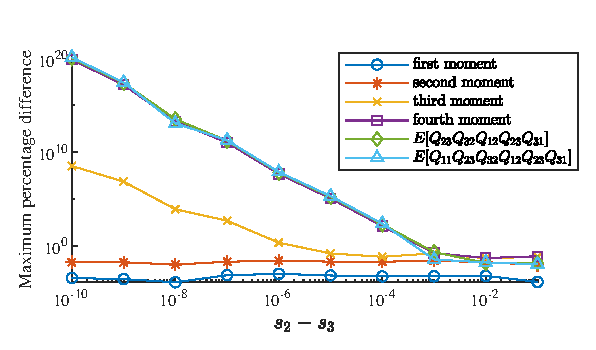
\includegraphics[scale=1.4]{figures/MF-moment-error-degenerate}
	\caption[Maximum difference between Monte Carlo method and the proposed recursive calculation when $s_2$ is close to $s_3$ for moments of the matrix Fisher distribution.]{Maximum difference between Monte Carlo method and the proposed recursive calculation when $s_2$ is close to $s_3$, with $s_1=25$, $s_2=10$.
	Double precision floating-point format is used in the recursive calculation. \label{fig:MF-moment-error-degenerate}}
\end{figure}

\section{Highly Concentrated Approximations of Matrix Fisher Distribution} \label{section:MF-approx}

The normalizing constant of the matrix Fisher distribution and its derivatives can be evaluated using the one dimensional integration formulae given in \eqref{eqn:MF-normalizing-1dInt} and $\eqref{eqn:MF-S2D-1dint}$, or using the saddle point approximation as discussed in \cite{gilitschenski2014efficient}.
However, these approaches are very computationally demanding.
Also, to inference the parameters $F$ from random samples, one must solve the partial differential equation in \eqref{eqn:MF-S2D}.
Because $d_i+d_j$ monotonically increases with $s_i+s_j$ for $i\neq j \in \{1,2,3\}$, and $d_i+d_j$ is upper bounded by 2, the average rate of change of $D$ with respect to $S$ becomes very small when $S$ is very large.
This makes \eqref{eqn:MF-S2D} extremely difficult to solve when $S$ has very large values.

However, large $S$ means the matrix Fisher distribution is highly concentrated.
As an analog of Gaussian distribution on $\SO{3}$, it can actually be approximated by a Gaussian distribution when $S$ is large.
This is similar to the von Mises and von Mises--Fisher distributions on $\Sph^n$ \cite{mardia2009directional}.
Nevertheless, since $\SO{3}$ has three degrees of freedom, the number of degrees of freedom in which the distribution is highly concentrated must be specified.
In the subsequent two subsections, the cases when the matrix Fisher distribution is highly concentrated in all three degrees of freedom, and in two degrees of freedom, are discussed.
And these approximations lead to simplifications of the normalizing constant, and its first order derivatives, which are computational costly to be evaluated.
The results can be further used to expedite the MLE of the parameter F, which requires solving the partial differential equation \eqref{eqn:MF-S2D} involving the normalizing constant.
Unfortunately, we were unable to give an approximation when the matrix Fisher distribution is only highly concentrated in one degree of freedom using the same strategy.

\subsection{Highly Concentrated in Three Degrees of Freedom}

As shown in \eqref{eqn:MF-density-principal}, the concentration of a matrix Fisher distribution along the $i$-th principal axis is controlled by $s_j+s_k$ for $i\neq j\neq k$.
Thus $s_1+s_2 \geq s_1+s_3 \geq s_2+s_3$, $s_2+s_3 \gg 0$ implies the distribution is highly concentrated in all three degrees of freedom.
The Gaussian approximation for this case has been studied in \cite{lee2018bayesian-b}, and is reviewed in this subsection.

\begin{theorem}[\cite{lee2018bayesian-b}] \label{thm:MF-approx-1d}
	Let $R\sim\mathcal{M}(F)$, where $F=USV^T$ is the pSVD of $F$.
	Suppose $s_2+s_3\gg 0$.
	Let $Q = U^TRV = \exp\left(\hat{\eta}\right)$, then $\eta \approxsim \mathcal{N}\big( 0,\allowbreak (\tr{S}I_{3\times 3}-S)^{-1} \big)$, where $\approxsim$ denotes ``approximately follows''.
\end{theorem}
\begin{proof}
	Let $\Sigma = (\tr{S}I_{3 \times 3}-S)^{-1} = \diag\left(\frac{1}{s_2+s_3},\frac{1}{s_1+s_3},\frac{1}{s_1+s_2}\right) \in\mathbb{R}^{3\times 3}$, and let $\xi\in\mathbb{R}^3$ be defined as $\sqrt{\Sigma}\xi = \eta$.
	Then the density \eqref{eqn:MF-density} for $R$ can be written as
	\begin{align*}
		&\etr{FR^T} = \etr{S\exp\left( (\sqrt{\Sigma}\xi)^\wedge \right)} \\
		=\; &\etr{S \Big( I_{3\times 3} + (\sqrt{\Sigma}\xi)^\wedge + \tfrac{1}{2} \big((\sqrt{\Sigma}\xi)^\wedge\big)^2 + O(\sqrt{\Sigma}) \Big)} \\
		=\; &\etr{\tfrac{1}{2}S\big((\sqrt{\Sigma}\xi)^\wedge\big)^2 + O(\sqrt{\Sigma})} \\
		\approx\; &\etr{S} \exp\left(-\tfrac{1}{2}\eta^T\Sigma^{-1}\eta\right).
	\end{align*}
	This finishes the proof.
\end{proof}

Theorem \ref{thm:MF-approx-1d} gives the following approximation of the normalizing constant.
\begin{corollary}[\cite{lee2018bayesian-b}] \label{cor:MF-normal-approx1}
	If $s_2+s_3\gg 0$, then
	\begin{align}
		c(S) &\approx \frac{\etr{S}}{\sqrt{8\pi(s_1+s_2)(s_1+s_3)(s_2+s_3)}} \label{eqn:MF-normalizing-approx1} \\
		\frac{1}{c(S)} \frac{\partial c(S)}{\partial s_i} &\approx 1 - \frac{1}{2}\left( \frac{1}{s_i+s_j} + \frac{1}{s_i+s_k} \right), \label{eqn:MF-S2D-approx1}
	\end{align}
	for $i,j,k\in\{1,2,3\}$ and $i\neq j\neq k$.
\end{corollary}
\begin{proof}
	According to \cite[Chapter 12.1.2]{chirikjian2011stochastic}, \eqref{eqn:MF-normalizing} can be written as
	\begin{align*}
		c(S) = \int_{\norm{\eta}<\pi} \etr{S\exp(\hat{\eta})} \frac{1-\cos\norm{\eta}}{4\pi^2\norm{\eta}^2} \diff\eta,
	\end{align*}
	where $\diff\eta$ is the Lebesgue measure on $\mathbb{R}^3$.
	Using the calculation in Theorem \ref{thm:MF-approx-1d}, and the Taylor expansion of $1-\cos x$, it can further be calculated as
	\begin{align*}
		c(S) &= \etr{S} \int_{\norm{\eta}<\pi} \expb{-\tfrac{1}{2} \eta^T \Sigma^{-1} \eta + O(\sqrt{\Sigma})} (1+O(\Sigma)) \tfrac{1}{8\pi^2} \diff\eta \\
		&\approx \int_{\mathbb{R}^3} \expb{-\tfrac{1}{2} \eta^T \Sigma^{-1} \eta}  \tfrac{1}{8\pi^2} \diff\eta.
	\end{align*}
	Then \eqref{eqn:MF-normalizing-approx1} can be obtained using the normalizing constant of $\mathcal{N}(0,\Sigma)$, and its derivation can also be calculated directly as \eqref{eqn:MF-S2D-approx1}.
\end{proof}

\begin{figure}
	\centering
	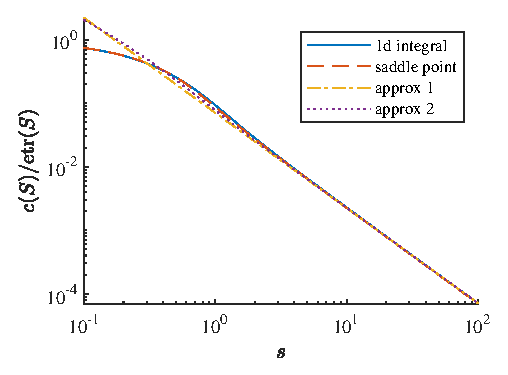
\includegraphics[scale=1.4]{figures/MF-normal-approx1}
	\caption[Comparison of the normalizing constant $c(S)$ calculated using different methods.]{Comparison of the normalizing constant $c(S)$ calculated using the one dimensional integral formula \eqref{eqn:MF-normalizing-1dInt}, the saddle point approximation \cite{kume2005saddlepoint}, the highly concentrated approximations \eqref{eqn:MF-normalizing-approx1} (approx 1) and \eqref{eqn:MF-normalizing-approx2} (approx 2).
	The parameter is $S = sI_{3\times 3}$.
	\label{fig:MF-nomral-approx1}}
\end{figure}

\begin{figure}
	\centering
	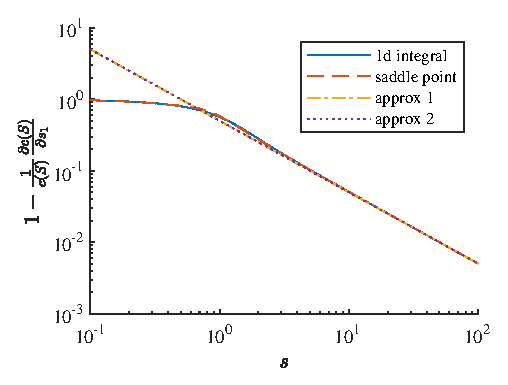
\includegraphics[scale=1.4]{figures/MF-S2D-approx1}
	\caption[Comparison of the first order moment $1-d_1$ calculated using different methods.]{Comparison of the first order moment $1-d_1$ calculated using the one dimensional integral formula \eqref{eqn:MF-S2D-1dint}, the saddle point approximation \cite{kume2005saddlepoint,kume2007derivatives}, the highly concentrated approximations \eqref{eqn:MF-S2D-approx1} (approx 1) and \eqref{eqn:MF-S2D-approx2-1} (approx 2).
	The parameter is $S = sI_{3\times 3}$.
	\label{fig:MF-S2D-approx1}}
\end{figure}

Corollary \ref{cor:MF-normal-approx1} provides a very fast computation for the normalizing constant $c(S)$ and its first order derivatives, using only basic functions.
Its accuracy is demonstrated in Figure \ref{fig:MF-nomral-approx1} against the one dimensional integral formula \eqref{eqn:MF-S2D-1dint}, and the saddle point approximation in \cite{kume2005saddlepoint}.
In addition, since the case when the matrix Fisher distribution is highly concentrated in two dimensions is a special case when it is highly concentrated in all three dimensions, the approximation in \eqref{eqn:MF-normalizing-approx2} is also compared.
The tested parameter is when $S = sI_{3\times 3}$, for $s$ ranging from 0.1 to 100.
It is shown that all calculations agree well when $s > 50$, whereas when $s < 50$, the two approximations deviate from the other two calculations, due to that the distribution is no longer highly concentrated.

The derivative of $c(S)$ is compared as $1-d_1 = 1-\tfrac{1}{c(S)} \tfrac{\partial c(S)}{\partial s_1}$ in Figure \ref{fig:MF-S2D-approx1}.
Again, all calculates are very close when $s>10$, but the two approximations become less accurate when the distribution is not highly concentrated.
It should be note that for extremely large $s$, for example when $s > 10^4$, the one dimensional integral formula, especially for the derivative \ref{eqn:MF-S2D-1dint}, becomes inaccurate when implemented with MATLAB \texttt{integral} function.

\subsection{Highly Concentrated in Two Degrees of Freedom} \label{section:MF-approx-2}

In this subsection, the case when $s_1+s_3\gg s_2+s_3 \geq 0$ is considered, i.e., the matrix Fisher distribution is highly concentrated along the second and third principal axes, but has large dispersion along the first axis.
Note that because $s_1 \geq s_2 \geq |s_3| \geq 0$, $s_1+s_3\gg s_2+s_3$ is equivalent to $s_1 \gg s_2$.
It is proved in this case, the matrix Fisher distribution can be approximated by a combination of a two dimensional Gaussian distribution in $\mathbb{R}^2$, and a one dimensional von Mises distribution on $\Sph^1$.

\begin{theorem} \label{thm:MF-approx-2d}
	Let $R\sim\mathcal{M}(F)$, where $F=USV^T$ is the pSVD of $F$.
	Suppose $s_1+s_3\gg 0$.
	Let $Q = U^TRV = \exp\left(\hat{\eta}\right) \exp\left(\hat{\eta}'\right)$, where $\eta = [0, \eta_2, \eta_3]^T$, and $\eta' = [\eta_1, 0, 0]^T$.
	Then $\eta_3 \approxsim \mathcal{VM}(0,s_2+s_3)$, and $ [\eta_2, \eta_3]^T  \approxsim \mathcal{N}\left( 0, \diag\left( \tfrac{1}{s_1+s_3}, \tfrac{1}{s_1+s_2} \right) \right)$, and they are approximately independent.
\end{theorem}
\begin{proof}
	let $\Sigma = \diag\left( 0, \tfrac{1}{s_1+s_3}, \tfrac{1}{s_1+s_2} \right)$, and $\eta = \sqrt{\Sigma} \xi$.
	Then $\exp\left(\hat{\eta}\right)$ can be written as
	\begin{align*}
		\exp\left(\hat{\eta}\right) = I_{3\times 3} + \sqrt{\Sigma}\hat{\xi} + \tfrac{1}{2} \left( \sqrt{\Sigma}\hat{\xi} \right)^2 + O\big(s_1^{-3/2}\big).
	\end{align*}
	Also, $\exp\left(\hat{\eta}'\right)$ can be explicitly calculated as
	\begin{align*}
		\exp\left(\hat{\eta}'\right) = \begin{bmatrix}
			1 & 0 & 0 \\
			0 & \cos\eta_1 & -\sin\eta_1 \\
			0 & \sin\eta_1 & \cos\eta_1
		\end{bmatrix}.
	\end{align*}
	Combining the above two equations, the density function for $R$ becomes
	\begin{align*}
		\etr{FR^T} &= \etr{S\exp(\hat{\eta})\exp(\hat{\eta}')} \\
		&= \exp(s_1) \cdot \exp((s_2+s_3)\cos\eta_1) \cdot \expb{-\tfrac{1}{2} \left( (s_1+s_3)\eta_2^2 + (s_1+s_2)\eta_3^2 \right)} \\
		&\quad \cdot \expb{-\tfrac{1}{2}\left( (s_2\eta_3^2 + s_3\eta_2^2)(\cos\eta_1-1) + (s_3-s_2)\eta_2\eta_3\sin\eta_1 \right) + O\big(s_1^{-1/2}\big)}.
	\end{align*}
	Note that the last exponential term can be simplified as
	\begin{align*}
		&(s_2\eta_3^2 + s_3\eta_2^2)(\cos\eta_1-1) + (s_3-s_2)\eta_2\eta_3\sin\eta_1 \\
		= &\left( \tfrac{s_2}{s_1+s_2}\xi_3^2 + \tfrac{s_3}{s_1+s_3}\xi_2^2 \right)(\cos\eta_1-1) + \tfrac{s_3-s_2}{\sqrt{s_1+s_3} \sqrt{s_1+s_2}} \xi_2\xi_3 \sin\eta_1 \\
		= & O\big(s_1^{-1}\big).
	\end{align*}
	So the density function for $R$ can be approximated by
	\begin{align*}
		\etr{FR^T} \approx \exp(s_1) \cdot \exp((s_2+s_3)\cos\eta_1) \cdot \expb{-\tfrac{1}{2} \left( (s_1+s_3)\eta_2^2 + (s_1+s_2)\eta_3^2 \right)},
	\end{align*}
	and the desired result is proved.
\end{proof}

Before looking into how this approximation can be applied to calculating the normalizing constant $c(S)$, a decomposition of the Haar measure $\diff Q$ on $\SO{3}$ needs to be introduced first \cite[Chapter 4]{dym1972fourier}.
Let $\mathbf{K} = \{\expb{\theta\hat{e}_1} \,|\, 0\leq \theta < 2\pi\}$ be a subgroup of $\SO{3}$, it is clear that $\mathbf{K}$ is isomorphic to $\SO{2} \cong \Sph^1$.
The quotient group of $\mathbf{K}$ is $\SO{3}/\mathbf{K} = \{ T\in\SO{3} \,|\, T\mathbf{K} \}$, which is isomorphic to $\Sph^2$ under the map
\begin{align} \label{eqn:SO3-SO3/K}
	j:\, \SO{3}/\mathbf{K} \to \Sph^2, \qquad T\mathbf{K} \mapsto Te_1.
\end{align}
Therefore, for any $Q\in\SO{3} = \SO{3}/\mathbf{K} \times \mathbf{K} \cong \Sph^2\times \Sph^1$, it can be decomposed as $Q = T(x) \expb{\theta\hat{e}_1}$,
for $x\in\Sph^2$ and $0\leq \theta< 2\pi$, where $T\mathbf{K} = j^{-1}(x)$.
And the Haar measure $\diff{Q}$ can be decomposed as $\tfrac{1}{8\pi^2} \diff \theta \diff \sigma(x)$, where $\diff \sigma(x)$ is the surface area measure on $\Sph^2$.
This decomposition can be used to obtain an approximation of the normalizing constant given in the next Corollary.

\begin{corollary}
	If $s_1+s_3 \gg s_2+s_3$, then
	\begin{align}
		c(S) &\approx \frac{\exp(s_1)I_0(s_2+s_3)}{2\sqrt{(s_1+s_2)(s_1+s_3)}}, \label{eqn:MF-normalizing-approx2} \\
		\frac{1}{c(S)}\frac{\partial c(S)}{\partial s_1} &\approx 1 - \frac{1}{2}\left( \frac{1}{s_1+s_2} + \frac{1}{s_1+s_3} \right), \label{eqn:MF-S2D-approx2-1} \\
		\frac{1}{c(S)}\frac{\partial c(S)}{\partial s_j} &\approx \frac{I_1(s_2+s_3)}{I_0(s_2+s_3)} - \frac{1}{2}\frac{1}{s_1+s_j}, \label{eqn:MF-S2D-approx2-2}
	\end{align}
	for $j\in\{2,3\}$.
\end{corollary}
\begin{proof}
	As shown in Theorem \ref{thm:MF-approx-2d}, $c(S)$ can be calculated as
	\begin{align*}
		c(S) \approx \exp(s_1) \int_{Q\in\SO{3}} \exp((s_2+s_3)\cos\eta_1) \cdot \expb{-\tfrac{1}{2} \left( (s_1+s_3)\eta_2^2 + (s_1+s_2)\eta_3^2 \right)} \diff Q
	\end{align*}
	Let $x = [\cos\alpha, \sin\alpha\cos\beta, \sin\alpha\sin\beta]^T \in \Sph^2$ be written in spherical coordinates, then using \eqref{eqn:SO3-SO3/K}, it can be shown that $j^{-1}(x) = \expb{\hat{\eta}} \mathbf{K}$, if $\eta$ is re-parameterized in polar coordinates as $\eta_2 = -\alpha\sin\beta$, $\eta_3 = \alpha\cos\beta$.
	Thus, $c(S)$ can be written as
	\begin{align*}
		c(S) &\approx \exp(s_1) \int_{0}^{2\pi} \exp((s_2+s_3)\cos\eta_1) \frac{1}{2\pi} \diff \eta_1 \\
		&\qquad \cdot \int_{0}^\pi \int_{0}^{2\pi} \expb{-\tfrac{1}{2} \left( (s_1+s_3)\eta_2^2 + (s_1+s_2)\eta_3^2 \right)} \frac{1}{4\pi} \sin\alpha \diff\beta \diff\alpha,
	\end{align*}
	where the first integral term is the normalizing constant of the von Mises distribution \cite[Chapter 3]{mardia2009directional}, given by $I_0(s_2+s_3)$.
	Note that $\eta_2 = \tfrac{\xi_2}{\sqrt{s_1+s_3}}$, and $\eta_3 = \tfrac{\xi_3}{\sqrt{s_1+s_2}}$, so $\sin\alpha = \alpha + O(s_1^{-3/2})$. Also, the integration for $\expb{-\tfrac{1}{2} \left( (s_1+s_3)\eta_2^2 + (s_1+s_2)\eta_3^2 \right)}$ becomes very small for $\alpha > \pi$ as $s_1+s_3 \gg 0$.
	Therefore, the second integral can be approximated by
	\begin{align*}
		&\int_0^\infty \int_{0}^{2\pi} \expb{-\tfrac{1}{2} \left( (s_1+s_3)\eta_2^2 + (s_1+s_2)\eta_3^2 \right)} \frac{1}{4\pi} \alpha \diff\beta \diff\alpha \\
		= &\int_{-\infty}^\infty \int_{-\infty}^\infty \expb{-\tfrac{1}{2} \left( (s_1+s_3)\eta_2^2 + (s_1+s_2)\eta_3^2 \right)} \frac{1}{4\pi} \diff\eta_2 \diff\eta_3,
	\end{align*}
	which is the normalizing constant of the Gaussian distribution.
	And \eqref{eqn:MF-normalizing-approx2} follows after combining the two integral terms.
	The derivatives \eqref{eqn:MF-S2D-approx2-1} and \eqref{eqn:MF-S2D-approx2-2} can be directly calculated by differentiating \eqref{eqn:MF-normalizing-approx2}.
\end{proof}

\begin{figure}
	\centering
	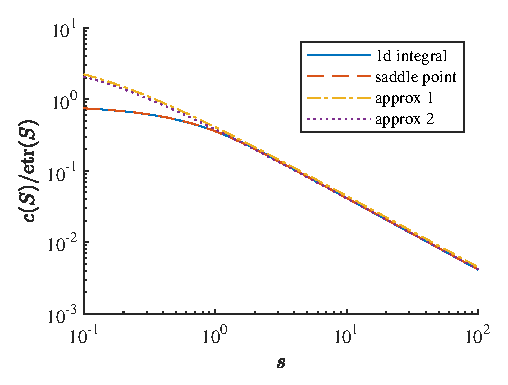
\includegraphics[scale=1.4]{figures/MF-normal-approx2}
	\caption[Comparison of the normalizing constant $c(S)$ calculated using different methods.]{Comparison of the normalizing constant $c(S)$ calculated using the one dimensional integral formula \eqref{eqn:MF-normalizing-1dInt}, the saddle point approximation \cite{kume2005saddlepoint}, the highly concentrated approximations \eqref{eqn:MF-normalizing-approx1} (approx 1) and \eqref{eqn:MF-normalizing-approx2} (approx 2).
	The parameter is $S = \diag(s,0.1,0.1)$.
	\label{fig:MF-nomral-approx2}}
\end{figure}

\begin{figure}
	\centering
	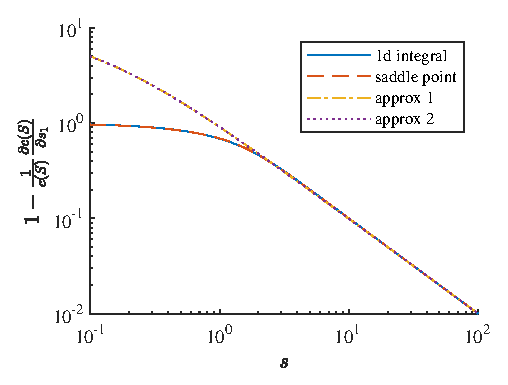
\includegraphics[scale=1.4]{figures/MF-S2D-approx2-1}
	\caption[Comparison of the first order moment $1-d_1$ calculated using different methods.]{Comparison of the first order moment $1-d_1$ calculated using the one dimensional integral formula \eqref{eqn:MF-S2D-1dint}, the saddle point approximation \cite{kume2005saddlepoint,kume2007derivatives}, the highly concentrated approximations \eqref{eqn:MF-S2D-approx1} (approx 1) and \eqref{eqn:MF-S2D-approx2-1} (approx 2).
	The parameter is $S = \diag(s,0.1,0.1)$.
	\label{fig:MF-S2D-approx2-1}}
\end{figure}

\begin{figure}
	\centering
	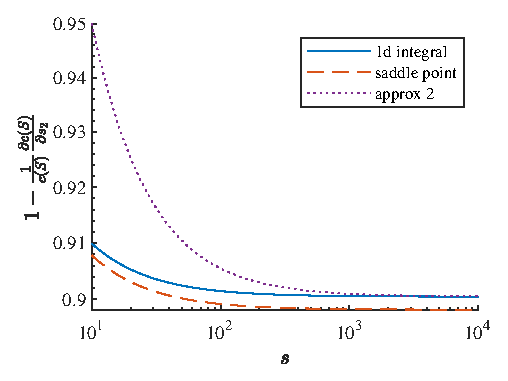
\includegraphics[scale=1.4]{figures/MF-S2D-approx2-2}
	\caption[Comparison of the first order moment $1-d_2$ calculated using different methods.]{Comparison of the first order moment $1-d_2$ calculated using the one dimensional integral formula \eqref{eqn:MF-S2D-1dint}, the saddle point approximation \cite{kume2005saddlepoint,kume2007derivatives}, the highly concentrated approximations \eqref{eqn:MF-S2D-approx2-2} (approx 2).
	The parameter is $S = \diag(s,0.1,0.1)$.
	\label{fig:MF-S2D-approx2-2}}
\end{figure}

Although the approximations \eqref{eqn:MF-normalizing-approx2} and \eqref{eqn:MF-S2D-approx2-2} involve the modified Bessel function of the first kind, then are much easier to be evaluated than $c(S)$ itself.
The comparision of $c(S)$ calculated from different methods is shown in Figure \ref{fig:MF-nomral-approx2}, for $S = \diag(s,0.1,0.1)$ with $s$ rangin from 0.1 to 100.
It can be seen that when $s>50$, the approximation \eqref{eqn:MF-normalizing-approx2} is very close to the one dimensional integral and saddle point approximation.
However, because $s_2+s_3 = 0.2$ is very small, the matrix Fisher distribution has very large dispersion in the first principal axis, and the approximation \eqref{eqn:MF-normalizing-approx1} developed for high concentration in all three degrees of freedom does not approximate $c(S)$ as well as \eqref{eqn:MF-normalizing-approx2}, even when $s_1 = s$ is large.

Next, the comparison of $1-d_1 = 1-\tfrac{1}{c(S)} \tfrac{\partial c(S)}{\partial s_1}$ is presented in Figure \ref{fig:MF-S2D-approx2-1}.
Similarly, the approximation \eqref{eqn:MF-S2D-approx2-1} becomes very close to the one dimensional integral and saddle point approximation.
And since \eqref{eqn:MF-S2D-approx1} is the same as \eqref{eqn:MF-S2D-approx2-1}, it also approximates the derivative well.
The comparison of $1-d_2 = 1-\tfrac{1}{c(s)}\tfrac{\partial c(S)}{\partial s_2}$ is presented in Figure \ref{fig:MF-S2D-approx2-2} for $S = \diag(s,0.1,0.1)$ with $s$ ranging from 10 to 10000.
It can be seen that the difference between the approximation \eqref{eqn:MF-S2D-approx2-2} and one dimensional integral becomes small when $s>500$.
The approximation \eqref{eqn:MF-S2D-approx1} for high concentration in all three degrees of freedom is not shown because its error is too large.
Also, it appears the that one dimensional integral is more accurate than the saddle point approximation, which is in general the case for $S$ that are not extremely large.

In summary, this chapter reviews the matrix Fisher and Bingham distributions that are used to model large uncertainty of 3D attitude.
A recursive algorithm is derived to calculate the central moments of the matrix Fisher distribution up to an arbitrary order.
Also, an approximation is proposed when the matrix Fisher distribution is highly concentrated in two degrees of freedom, which is used to derive simplified expressions for the normalizing constant and its derivatives.

% !TEX root = ../thesis-WW.tex

\chapter{Matrix Fisher-Gaussian Distribution} \label{chap:MFG}



% !TEX root = ../thesis-WW.tex

\chapter{Bayesian Estimation with Matrix Fisher-Gaussian Distribution} \label{chap:estimation}

In the previous two chapters, the matrix Fisher distribution defined on $\SO{3}$ is reviewed, and a new probability model called the matrix Fisher--Gaussian distribution on $\SO{3}\times \mathbb{R}^n$ is developed to model the correlation between $\SO{3}$ and $\mathbb{R}^n$.
The development of MFG opens a new gate to use the matrix Fisher distribution or Bingham distribution in a lot of classic estimation problems where the attitude and some quantities in Euclidean space must be estimated simultaneously, such as position, sensor biases, landmark locations, etc.
Compared to MEKF and its variants \cite{mourikis2007multi,sola2017quaternion}, the stochastic estimator designed using MFG has the potential to handle large attitude uncertainty, which may occur when the initial conditions are unknown, when there is a degree of freedom in attitude that is not properly observed, or when some sensors fail (for example a GPS receiver) for a long period of time.
The fact that MFG models large attitude uncertainty with high fidelity could make the estimator achieve higher accuracy, or faster convergence speed from a wrong state.

In this chapter, this idea is investigated with three estimation problems: (i) attitude estimation with a gyroscope and direction sensors, (ii) loosely coupled IMU-GNSS system for localization, and (iii) visual-inertial odometry or localization.
First in Chapter \ref{section:observability}, the observability of 3D attitude is studied when only angular velocity and single direction measurements are available, where the matrix Fisher distribution is utilized to analyze how the attitude uncertainty is propagated through the gyroscope kinematics, and updated by the single direction measurement.
Then in Chapter \ref{section:attEst}, a new recursive Bayesian filter based on MFG is designed to estimate the attitude and gyroscope bias simultaneously.
In particular, the linear part of MFG is used to model the gyroscope bias in $\mathbb{R}^3$.
In Chapter \ref{section:posEst}, attitude estimation is generalized into a full inertial navigation problem, where the linear acceleration measured by an accelerometer is transformed into the inertial frame using the estimated attitude, and integrated twice into position.
Under this setting, the linear part of MFG is augmented into $\mathbb{R}^{12}$, including the linear velocity, position, gyroscope and accelerometer biases.
The measurement update is considered with position measurements given by a GNSS receiver.
Finally in Chapter \ref{section:VIO}, the position measurement is replaced by camera measurements of the locations for unknown features or known landmarks.
It is assumed that the camera is an RGB-D or stereo camera, so that projection measurements have already been triangulated into 3D locations.

It is demonstrated in this chapter that the estimators designed using MFG have advantages over MEKF or its variants when dealing with unknown initial conditions, and when not all degrees of freedom for attitude are adequately observed.
In particular, the MFG based filter has faster convergence speed from large initial errors, highlighting its capability to model large attitude uncertainty with high fidelity.

\section{Attitude Observability with Single Direction Measurement} \label{section:observability}

In this section, the matrix Fisher distribution is used to study the observability of attitude when the angular velocity, and a single reference direction are measured.
Because the attitude has three degrees of freedom, and a single direction measurement fixes two of them, at least two reference directions are needed to fully determine the 3D attitude \cite{markley1988attitude,shuster1981three}.
This is widely believed to be the case even when the angular velocity is also measured \cite{mahony2008nonlinear}, except in a few special cases, for example, when the single reference direction is time-varying in the inertial frame \cite{batista2012ges,grip2011attitude,lee2007global}, and when the gyroscope can capture the rotation of the earth \cite{reis2018nonlinear}.
However, there is no available explanation on why introducing the information of angular velocity measurement does not improve the observability of attitude with single direction measurements.

In this section, this problem is studied by examining how the attitude uncertainty is propagated through the attitude kinematics, and how it is shaped by injecting the information from single direction measurements.
In particular, it is shown that the attitude uncertainty is propagated in different ways, depending on whether the angular velocity is measured in the body-fixed frame or in the inertial frame.
For the former, the direction of one-dimensional ambiguity caused by a single direction measurement remains fixed in the inertial frame, but for the latter, it is fixed in the body-fixed frame.
This explains the fundamental reason why the attitude is unobservable with a single inertial reference direction and the angular velocity measured by a gyroscope: the direction of ambiguity caused by the inertial reference direction measurement remains unchanged by the angular velocity resolved in the body-fixed frame.
This leads to two strategies to achieve full attitude observability with single direction measurements, namely utilizing the angular velocity resolved in the inertial frame such that the direction of ambiguity is rotated over propagation, or measuring a reference direction fixed to the body such that the next measurement can resolve the ambiguity.
These results are summarized in Table \ref{table:observability}.

\begin{table}
	\caption{\label{table:observability} Attitude observability with single direction measurements}
	\centering
	\begin{tabular}{l|cc}
		\diagbox[width=10em]{ref. vec.}{ang. vel.} & body-fixed frame & inertial frame \\ \hline
		body-fixed frame &  observable & unobservable \\
		inertial frame & unobservable & observable
	\end{tabular}
\end{table}

This discovery is more rigorously studied by introducing two formulations of stochastic attitude observability.
For a given probability density function on $\SO{3}$, the attitude that minimizes the mean square error may not be unique~\cite{moakher2002means,pennec2006intrinsic}.
This gives a characterization of the attitude observability, since if multiple attitudes can minimize the mean square error, it indicates deficiency of information to distinguish them.
Alternatively, the inverse of Fisher information gives a lower bound for the variance of all unbiased estimators, known as the Cram\'{e}r--Rao bound, and the observability can be characterized by the positive-definiteness of the Fisher information matrix \cite{mohler1988nonlinear}.
The method in \cite{smith2005covariance} which generalizes the Fisher information to Riemannian manifold is used to calculate the Fisher information of the mean attitude of a matrix Fisher distribution.
It is further shown that the two attitude observability criteria are consistent with each other, and they also agree with a classic deterministic observability analysis when only a single direction measurement is available.

\subsection{Problem Formulation}

In this section, a vector is denoted by a bold lower-case letter, and it is distinguished with its coordinates in some coordinate frame.
The inertial frame is defined by its three orthogonal axes $\mathbf{I} = \{\bm{e}_1, \bm{e}_2, \bm{e}_3\}$.
And the coordinates of $\bm{e}_i$ in $\mathbf{I}$ is $e_i$, i.e., the $i$-th column of $I_{3\times 3}$, for $i=1,2,3$.
Similarly, the body fixed frame is defined as $\mathbf{B} = \{\bm{b}_1, \bm{b}_2, \bm{b}_3\}$.
A rotation matrix $R\in\SO{3}$ is used to transform the coordinates of a vector from the body fixed frame to the inertial frame.

The following stochastic attitude kinematics is studied:
\begin{align}
	dR = (\omega(t) dt + H(t) dW)^\wedge R, \label{eqn:observability-kinematics-right} \\
	dR = R (\Omega(t) dt + H(t) dW)^\wedge, \label{eqn:observability-kinematics-left}
\end{align}
where the angular velocity $\omega(t)$ is resolved in $\mathbf{I}$, and $\Omega(t)$ is resolved in $\mathbf{B}$, and they are assumed to be given as deterministic functions of time.
The angular velocity is perturbed by the additive noise $H(t)dW$, which is a Wiener process $W\in\mathbb{R}^3$ scaled by a matrix $H(t)\in\mathbb{R}^{3\times 3}$. 
The above stochastic differential equations are defined according to the Stratonovich sense so that the random matrix $R$ evolves on $\SO{3}$ \cite{barrau2018stochastic}, and they are called \textit{right-trivialized} and \textit{left-trivialized}, respectively.

Next, two types of direction measurements are also considered.
The first type is referred to as \textit{inertial direction measurement}, when the reference direction is known in the inertial frame, and the measurement output is resolved in the body-fixed frame.
More specifically, let $\bm{a}$ be a reference vector fixed in the inertial frame, and $a\in\Sph^2$ be its coordinates in the inertial frame.
The reference direction is measured with a sensor fixed to the body, which provides the measurement $x\in\Sph^2$ resolved in the body-fixed frame. 
It is assumed that the sensor measurement for a given attitude is distributed according to the von Mises-Fisher distribution on $\Sph^2$ as follows:
\begin{align} \label{eqn:observability-measurement-inertial}
	p(x|R) = \frac{\kappa}{4\pi\sinh \kappa} \exp( \kappa a^T Rx),
\end{align}
where the mean is $R^Ta\in\Sph^2$, and $\kappa>0$ is the concentration parameter.
On the contrary, the second type of direction measurement is referred to as \textit{body-fixed direction measurement}, when the reference direction is known in the body-fixed frame, and the measurement output is resolved in the inertial frame.
In other words, a reference vector $\bm{b}$ fixed to the body with the coordinates $b\in\Sph^2$ in the body-fixed frame, is measured by a sensor as $y\in\Sph^2$ resolved in the inertial frame.
And $y|R$ is assumed to be distributed by
\begin{align} \label{eqn:observability-measurement-body}
	p(y|R) = \frac{\kappa}{4\pi\sinh \kappa} \exp( \kappa b^T R^T y).
\end{align}

It is assumed that the reference direction is repeatedly measured at discrete time instants $\{t_k\}_{k=1}^\infty$, with a fixed time step $h = t_{k+1}-t_k$.
This section studies the observability of $R$ when the continuous attitude kinematics \eqref{eqn:observability-kinematics-right} or \eqref{eqn:observability-kinematics-left} is combined with the single direction measurements \eqref{eqn:observability-measurement-inertial} or \eqref{eqn:observability-measurement-body}.
The approach is to investigate how the attitude uncertainty is propagated between measurements by the noisy angular velocity measurement, and how the single direction measurement injects information into the uncertainty.

\subsection{Uncertainty Propagation} \label{section:observability-propagation}

Although the continuous kinematics \eqref{eqn:observability-kinematics-right} and \eqref{eqn:observability-kinematics-left} can be directly analyzed \cite{wang2020observability}, for simplicity, the discretized versions of them is studied here.
As shown in \cite{barrau2018stochastic}, the solutions of
\begin{align}
	R_{k+1} &= \exp\!\big( h\hat{\omega}_k + (H_k\Delta W)^\wedge \big) R_k \label{eqn:observability-kinematics-right-dist}, \\
	R_{k+1} &= R_k \exp\!\big( h\hat{\Omega}_k + (H_k\Delta W)^\wedge \big) \label{eqn:observability-kinematics-left-dist}
\end{align}
converge in probability to the solutions of the continuous equations \eqref{eqn:observability-kinematics-right} and \eqref{eqn:observability-kinematics-left} as $h\to 0$, respectively, where $\Delta W$ is the stochastic increment of $W$ over the time step $h$.
It is further assumed the noise is isotropic \cite{barrau2018stochastic}, i.e., $H_k = \gamma I_{3\times 3}$ for $\gamma >0$.
Unfortunately, there is no explicit analytical solution to the stochastic difference equations \eqref{eqn:observability-kinematics-right-dist} and \eqref{eqn:observability-kinematics-left-dist}.
Instead, we study how the first moment of $R$ evolves, and interpret its uncertainty utilizing the matrix Fisher distribution.

Specifically, the moments $\expect{R_k}$ for the right-trivialized \eqref{eqn:observability-kinematics-right-dist} and left-trivialized \eqref{eqn:observability-kinematics-left-dist} are propagated into $\expect{R_{k+1}}$ according to the following theorem.

\begin{theorem}
	Suppose $R$ follows the right-trivialized stochastic difference equation \eqref{eqn:observability-kinematics-right-dist}, then
	\begin{align} \label{eqn:observability-kinematics-ER_R}
		\expect{R_{k+1}}_R = (1-h\gamma^2) \exp(h\hat{\omega}_k) \expect{R_k} + O(h^2).
	\end{align}
	If instead $R$ follows the left-trivialized \eqref{eqn:observability-kinematics-left-dist}, then
	\begin{align} \label{eqn:observability-kinematics-ER_L}
		\expect{R_{k+1}}_L = (1-h\gamma^2) \expect{R_k} \exp(h\hat{\Omega}_k) + O(h^2).
	\end{align}
\end{theorem}
\begin{proof}
	By the Baker–Campbell–Hausdorff formula, \eqref{eqn:observability-kinematics-right-dist} can be written as
	\begin{align*}
		R_{k+1} = \exp(h\hat{\omega}_k) \exp\!\big( (H_k\Delta W)^\wedge + O(h\Delta W) \big) R_k.
	\end{align*}
	Expanding the exponential term in the middle of the right hand side, and noting that $\expect{\Delta W} = 0$, it can be shown that
	\begin{align*}
		\expect{\exp\!\big( (H_k\Delta W)^\wedge + O(h\Delta W) \big)} 
		&= I_{3\times 3} + \tfrac{1}{2} \expect{\big((H_k\Delta W)^\wedge + O(h\Delta W)\big)^2} + O(h^2) \\
		&= (1-h\gamma^2)I_{3\times 3} + O(h^2),
	\end{align*}
	where the second equality used $\expect{\Delta W\Delta W^T} = hI_{3\times 3}$ and \eqref{eqn:SO3-hatx^2}.
	The left-trivialized \eqref{eqn:observability-kinematics-ER_L} can be derived similarly.
\end{proof}

In \eqref{eqn:observability-kinematics-ER_R} and \eqref{eqn:observability-kinematics-ER_L}, the propagation of the first moment of $R$ from $t_k$ to $t_{k+1}$ is composed of two parts: the exponential term corresponds to the advection, or the rotation of the distribution, due to the deterministic angular velocity, which acts on the left or on the right of the original expectation depending on whether the right- or left- trivialized kinematics is used; and the scalar $1-h\gamma^2$ represents the diffusion due to noise.

The expectation of $R$ is interpreted using the matrix Fisher distribution.
Suppose $R_k \sim \mathcal{M}(F_k)$ with $F_k = U_k S_k V_k^T\in\mathbb{R}^{3\times 3}$.
From \eqref{eqn:MF-S2D}, its first moment is given by $\expect{R_k} = U_k D_k V_k^T$.
Therefore, \eqref{eqn:observability-kinematics-ER_R} and \eqref{eqn:observability-kinematics-ER_L} are rewritten as 
\begin{align*}
	\expect{R_{k+1}}_R &= \exp(h\hat\omega_k) U_k \times (1-h\gamma^2)D_k \times V_k^T, \\
	\expect{R_{k+1}}_L &= U_k \times (1-h\gamma^2)D_k \times (\exp(-h\hat{\Omega}_k)V_k)^T
\end{align*}
respectively, after omitting the higher order terms of $h$.
We assume $R_{k+1} \sim \mathcal{M}(F_{R_{k+1}})$ for \eqref{eqn:observability-kinematics-right-dist}, and $R_{k+1} \sim \mathcal{M}(F_{L_{k+1}})$ for \eqref{eqn:observability-kinematics-left-dist}, with the pSVD of the parameters given by $F_{R_{k+1}} = U_{R_{k+1}}S_{R_{k+1}}V_{R_{k+1}}^T$, and $F_{L_{k+1}} = U_{L_{k+1}}S_{L_{k+1}}V_{L_{k+1}}^T$.
Then using the MLE for matrix Fisher distribution, for \eqref{eqn:observability-kinematics-right-dist} it can be shown that
\begin{align} \label{eqn:observability-kinematics-UV_R}
	U_{R_k+1} = \exp(h\hat{\omega}_k)U_k, \quad V_{R_{k+1}} = V_k,
\end{align}
and for \eqref{eqn:observability-kinematics-left-dist} the estimation becomes
\begin{align}
	U_{L_{k+1}} = U_k, \quad V_{L_{k+1}} = \exp(-h\hat{\Omega}_k)V_k.
\end{align}
Next, for both of \eqref{eqn:observability-kinematics-right-dist} and \eqref{eqn:observability-kinematics-left-dist},
\begin{align} \label{eqn:observability-kinematics-S}
	S_{R_{k+1}} = S_{L_{k+1}} = \mathcal{E}^{-1}\big((1-h\gamma^2)D_k\big) \triangleq S_{k+1},
\end{align}
where $\mathcal{E}^{-1}$ denotes solving $S$ from $D$ using \eqref{eqn:MF-S2D}.

Now, the uncertainty propagation of $R$ is considered in three aspects: the mean attitude, the degree of dispersion, and the principal axes. 
First, the mean attitude is rotated from $M_k = U_k V_k^T$ into
\begin{align}
	M_{R_{k+1}} &= U_{R_{k+1}} V_{R_{k+1}}^T = \exp(h\hat\omega_k ) U_k V_k^T, \label{eqn:M_kp_R} \\
	M_{L_{k+1}} &= U_{L_{k+1}} V_{L_{k+1}}^T =  U_k V_k^T \exp(h\hat\Omega_k), \label{eqn:M_kp_L}
\end{align}
for \eqref{eqn:observability-kinematics-right-dist} and \eqref{eqn:observability-kinematics-left-dist} respectively, which is rotated by the deterministic angular velocity as expected.
If the angular velocities are transformed to each other by the mean attitude at $t_k$, then the propagated mean attitudes are identical, i.e., 
$\Omega_k = (U_kV_k^T)^T \omega_k$ implies $M_{R_{k+1}} = M_{L_{k+1}}$.
Second, the uncertainty becomes more dispersed in the same manner for \eqref{eqn:observability-kinematics-right-dist} and \eqref{eqn:observability-kinematics-left-dist}, as $S_{k+1}$ is reduced from $S_k$ according to \eqref{eqn:observability-kinematics-S} and Lemma \ref{lemma:MF-SD}.

Finally, the most notable distinction between \eqref{eqn:observability-kinematics-right-dist} and \eqref{eqn:observability-kinematics-left-dist} is how the principal axes are rotated.
For \eqref{eqn:observability-kinematics-right-dist}, since $U_{R_{k+1}} = \exp(h\hat\omega_k) U_k$, the principal axes are rotated by the rotation vector $h\omega_k$ when perceived in the inertial frame.
However, as $V_{R_{k+1}} = V_k$, the principal axes remain unchanged when observed from the body-fixed frame.
For \eqref{eqn:observability-kinematics-left-dist}, it is exactly the opposite: since $V_{L_{k+1}} = \exp(-h\hat\Omega_k) V_k$, the principal axes are rotated by the rotation vector $-h\Omega_k$ when perceived in the body-fixed frame, and they remain unchanged when observed from the inertial frame.
In other words, for \eqref{eqn:observability-kinematics-right-dist}, the shape of uncertainty represented by the most and least uncertain directions remains fixed in the body-fixed frame, but it is rotated in the inertial frame.
On the other hand, for \eqref{eqn:observability-kinematics-left-dist}, the most and least uncertain directions are rotated in the body-fixed frame, but they are fixed in the inertial frame.
These are illustrated in Figure \ref{fig:observability-kinematics}.

\begin{figure}
	\centering
	\begin{tikzpicture}
		\node at (2.5,5) {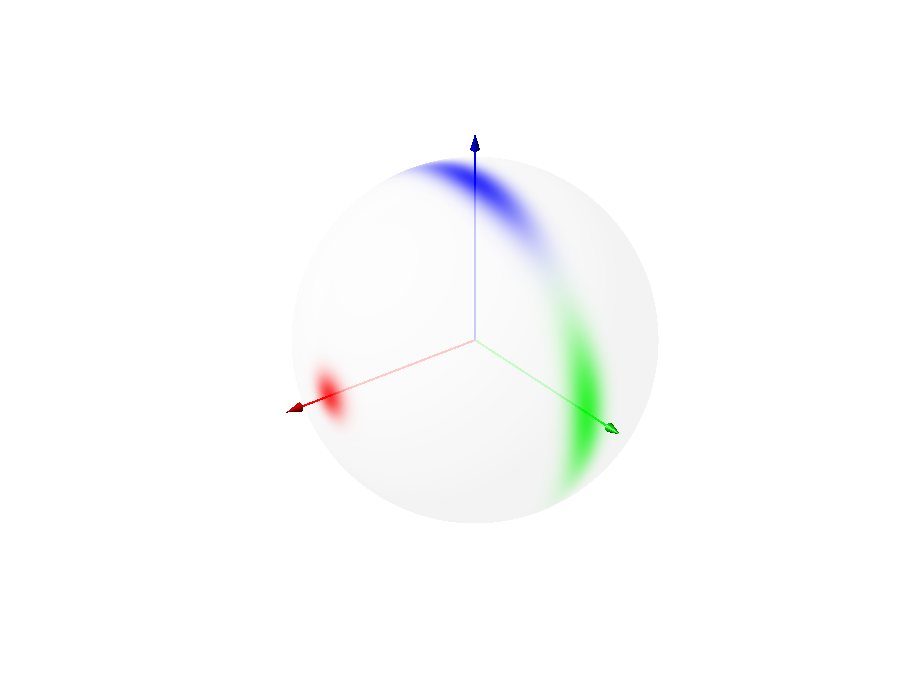
\includegraphics[trim=100 70 100 30, clip, scale=0.65]{figures/observability/prop_R_1}};
		\node at (7.5,5) {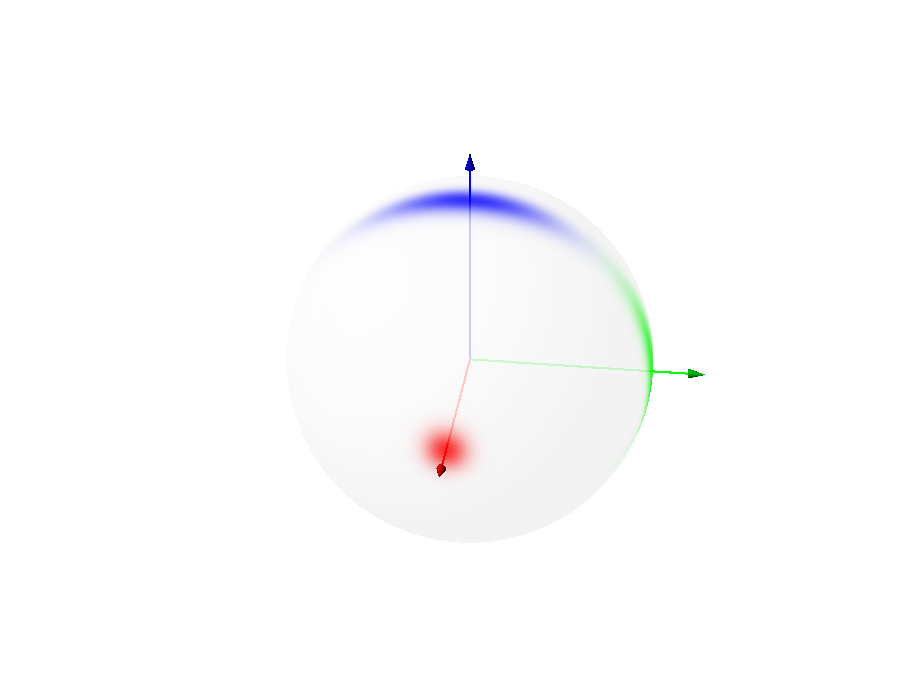
\includegraphics[trim=100 60 100 40, clip, scale=0.65]{figures/observability/prop_R_2}};
		\node at (12.5,5) {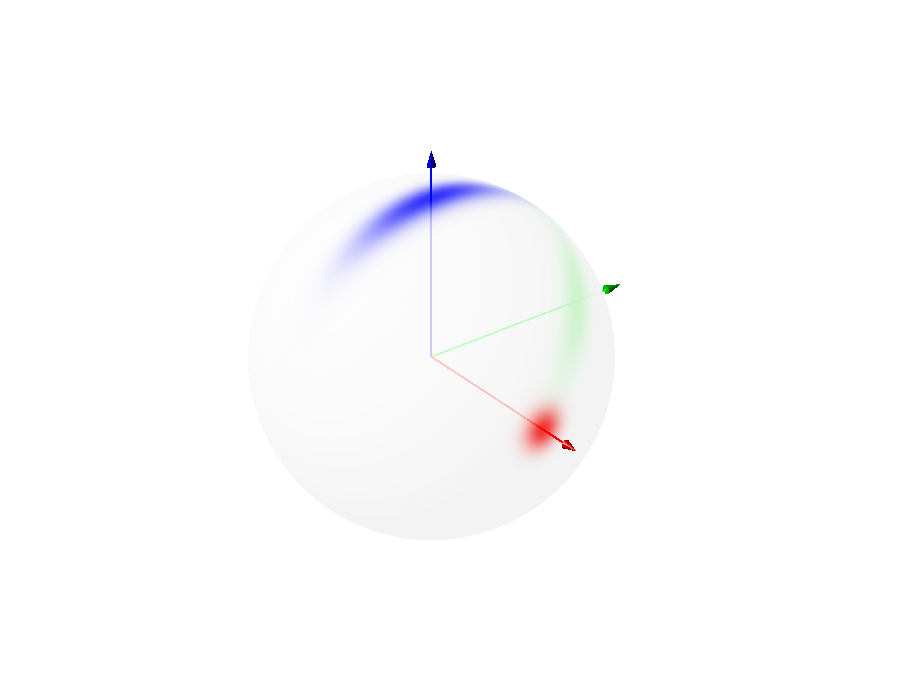
\includegraphics[trim=100 60 100 40, clip, scale=0.65]{figures/observability/prop_R_3}};
		
		\node at (2.5,0) {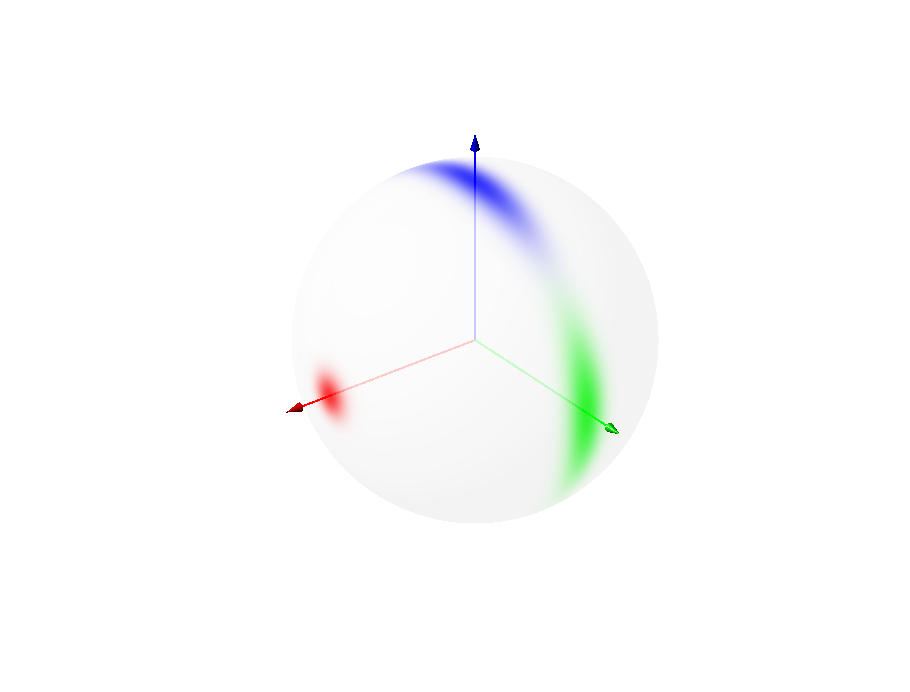
\includegraphics[trim=100 70 100 30, clip, scale=0.65]{figures/observability/prop_L_1}};
		\node at (7.5,0) {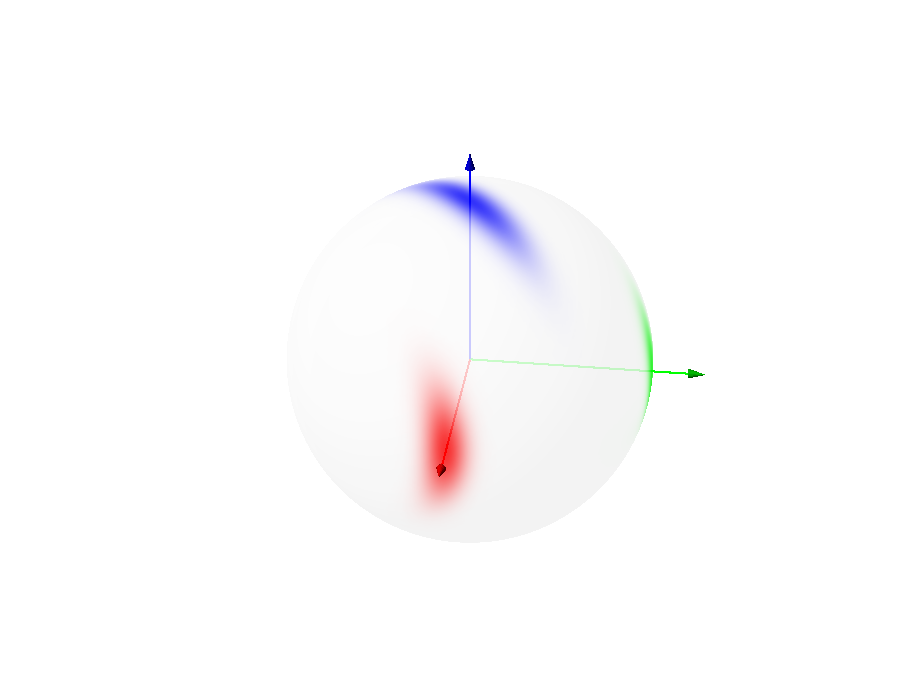
\includegraphics[trim=100 60 100 40, clip, scale=0.65]{figures/observability/prop_L_2}};
		\node at (12.5,0) {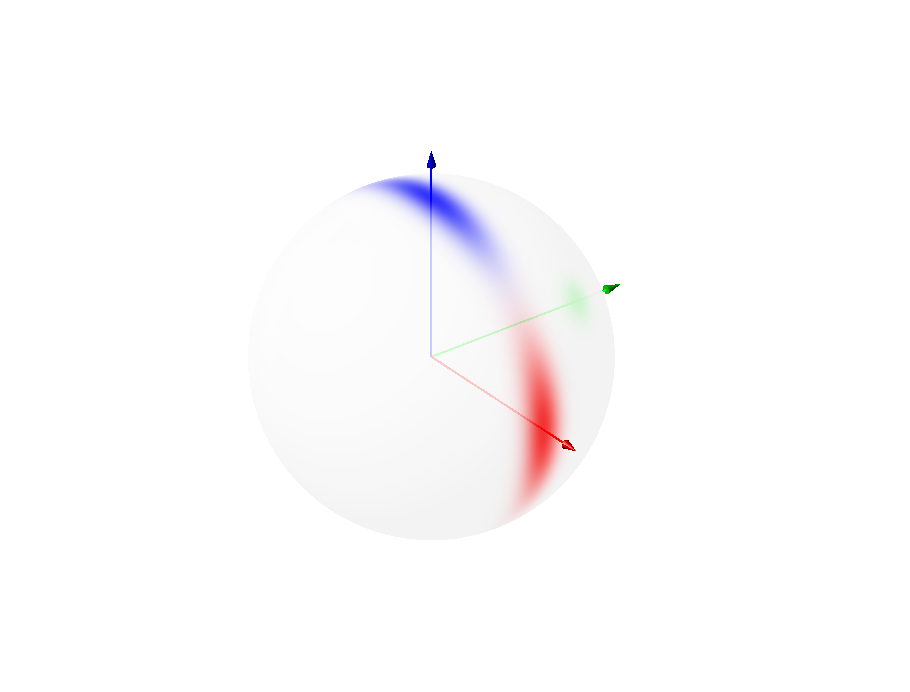
\includegraphics[trim=100 60 100 40, clip, scale=0.65]{figures/observability/prop_L_3}};
		
		\node at (0,4.85) {\rotatebox{90}{right-trivialized \eqref{eqn:observability-kinematics-right-dist}}};
		\node at (0,-0.3) {\rotatebox{90}{left-trivialized \eqref{eqn:observability-kinematics-left-dist}}};
		
		\draw[arrows={-Triangle[angle=30:8pt]}] (5.25,2.7) -- ++(90:0.8);
		\draw[arrows={-Triangle[angle=30:8pt]}] (5.25,2.7) -- ++(-30:0.8);
		\draw[arrows={-Triangle[angle=30:8pt]}] (5.25,2.7) -- ++(210:0.8);
		\node at (4.35,2.3) {$\bm{e}_1$};
		\node at (6.25,2.3) {$\bm{e}_2$};
		\node at (5.25,3.7) {$\bm{e}_3$};
		
		\node at (0.8,6.5) {(a)};
		\node at (5.8,6.5) {(b)};
		\node at (10.8,6.5) {(c)};
		\node at (0.8,1.55) {(d)};
		\node at (5.8,1.55) {(e)};
		\node at (10.8,1.55) {(f)};
		
		\node at (2.8,-3.0) {$t=0$s};
		\node at (7.7,-3.0) {$t=0.5$s};
		\node at (12.3,-3.0) {$t=1$s};
	\end{tikzpicture}

	\caption[Illustration of propagated uncertainties by the right-trivialized \eqref{eqn:observability-kinematics-right-dist} and the left-trivialized \eqref{eqn:observability-kinematics-left-dist}.]{Illustration of propagated uncertainties: (a-c) by the right-trivialized \eqref{eqn:observability-kinematics-right-dist}; (d-f) by the left-trivialized \eqref{eqn:observability-kinematics-left-dist}.
		The initial distribution is $R_0 \sim \mathcal{M}(F_0)$ with $F_0 = \diag(150, 10, 0)$.
		The angular velocities are $\omega = \Omega = \tfrac{\pi}{2}e_3 \SI{}{\radian\per\second}$ without any noise, which can be transformed to each other by the initial mean attitude $I_{3\times 3}$.
		The red, green and blue arrows represent the mean directions of the body-fixed $\bm{b}_1$, $\bm{b}_2$, $\bm{b}_3$ axes, and the corresponding shades represent the marginal distribution for each body-fixed axis.
		It can be observed that the mean attitude and the degree of dispersion are consistent between \eqref{eqn:observability-kinematics-right-dist} and \eqref{eqn:observability-kinematics-left-dist}.
		However, for \eqref{eqn:observability-kinematics-right-dist}, the most uncertain direction is fixed along the body-fixed $\bm{b}_1$ axis (red), but it is rotated in the inertial frame; and the most uncertain direction for \eqref{eqn:observability-kinematics-left-dist} is rotated in the body-fixed frame (from red to green), but it remains fixed along the inertial $\bm{e}_1$ axis, thereby causing all of the shades circular about $\bm{e}_1$.
	}
	\label{fig:observability-kinematics}
\end{figure}

\subsection{Measurement Update} \label{section:observability-measurement}

This subsection examines how the single direction measurements \eqref{eqn:observability-measurement-inertial} and \eqref{eqn:observability-measurement-body} are used to update the uncertainty propagated from the previous time step.
The additional information in the direction measurement is injected into the prior uncertainty by calculating the conditional distribution $R|x$ or $R|y$, using Bayes' formula. 
\begin{theorem} \label{thm:F_post}
	Let $R\sim\mathcal{M}(F^-)$ be a prior distribution for a given $F^-\in\mathbb{R}^{3\times 3}$.
	Then, for the inertial direction measurement, the posterior distribution of the attitude conditioned by $x$ is also matrix Fisher with $R|x \sim \mathcal{M}(F_I^+)$, where the posterior matrix parameter $F_I^+\in\mathbb{R}^{3\times 3}$ is given by
	\begin{align}
		F_I^+ = F^- + \kappa a x^T.\label{eqn:observability-measurement-F_I}
	\end{align}
	And for the body-fixed direction measurement, the posterior distribution is $R|y \sim \mathcal{M}(F_B^+)$, where $F_B^+\in\mathbb{R}^{3\times 3}$ is given by
	\begin{align}
		F_B^+ = F^- + \kappa y b^T.\label{eqn:observability-measurement-F_B}
	\end{align}
\end{theorem}
\begin{proof}
	The proof for inertial direction measurement is given in Theorem 3.2 of \cite{lee2018bayesian}, and the body-fixed direction measurement can be derived similarly.
\end{proof}

\begin{figure}
	\centering
	\begin{tikzpicture}
		\node at (2.4,5.5) {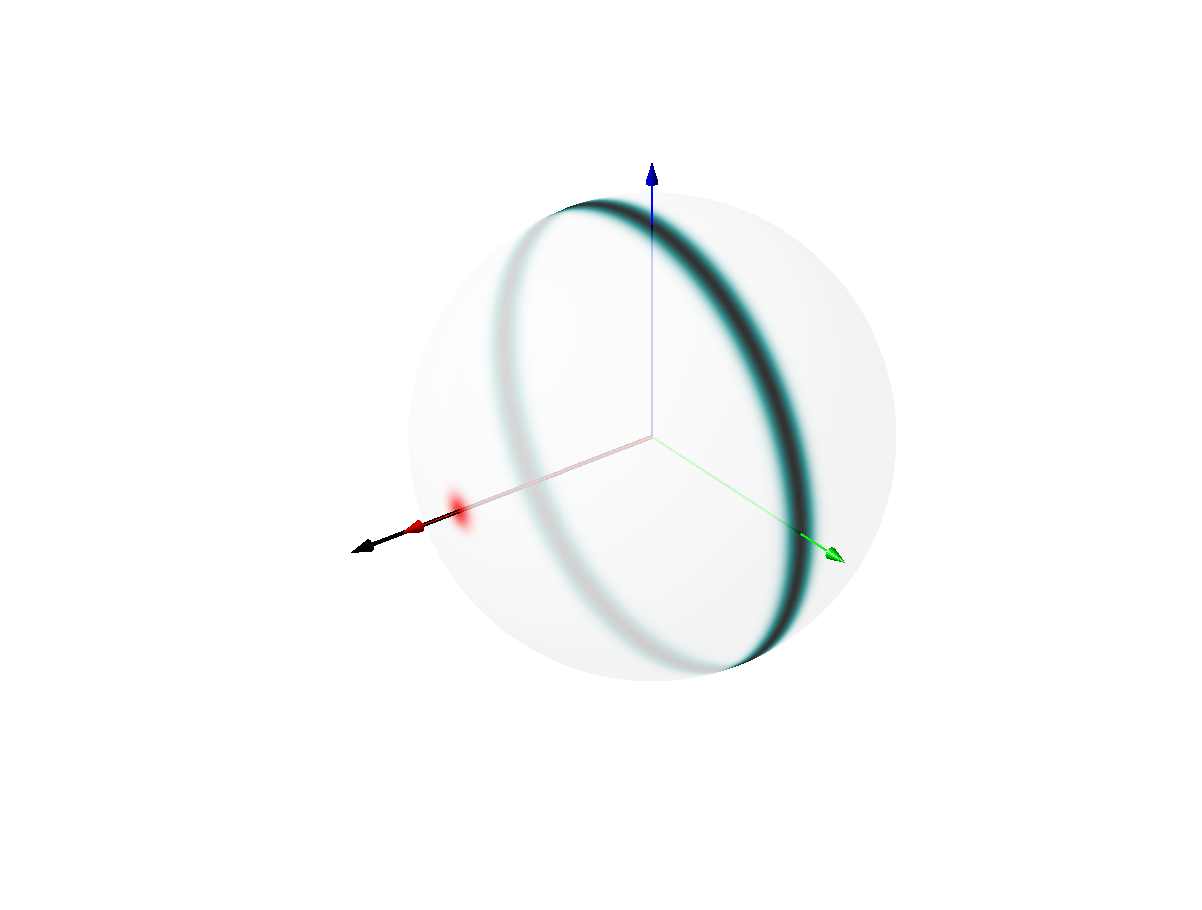
\includegraphics[trim=130 80 120 60, clip, scale=0.45]{figures/observability/mea_I_1}};
		\node at (7.3,5.5) {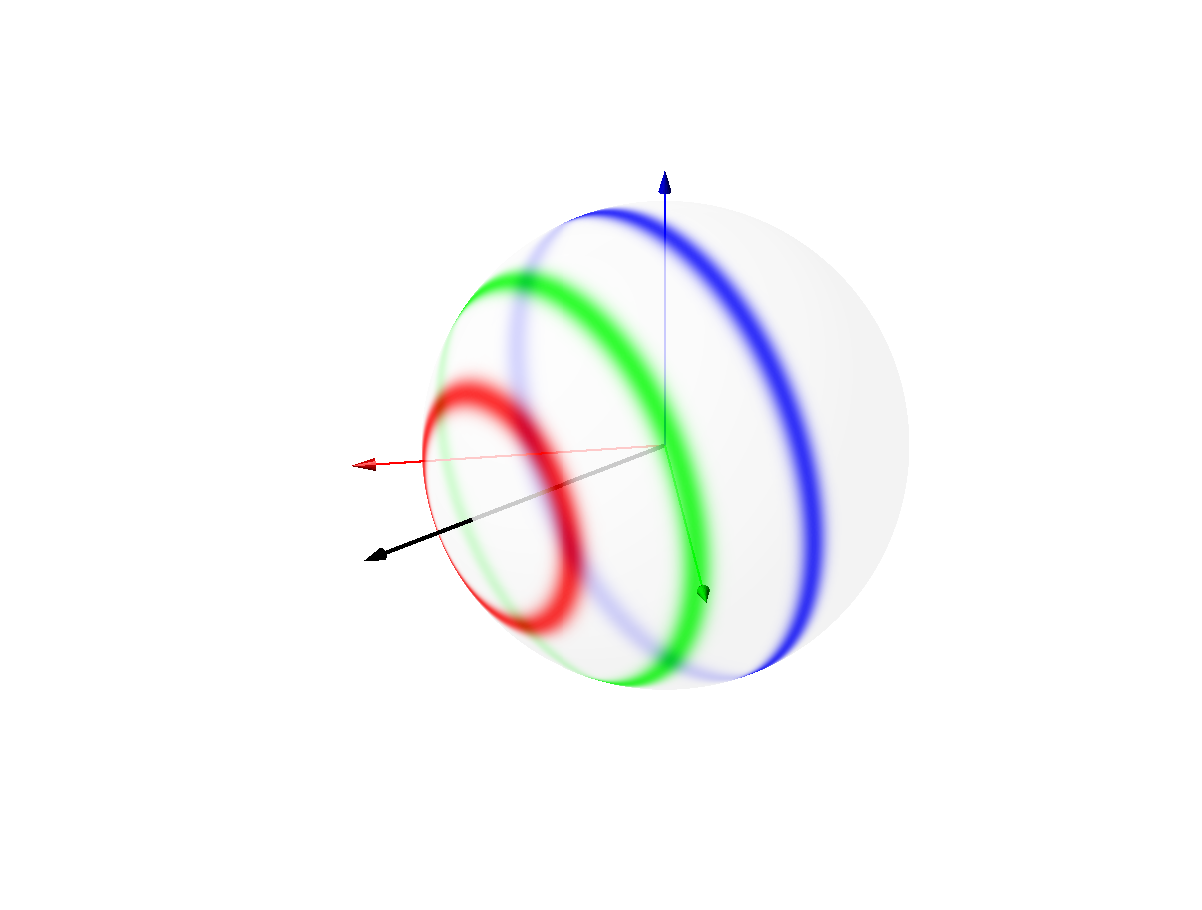
\includegraphics[trim=130 80 120 60, clip, scale=0.45]{figures/observability/mea_I_2}};
		\node at (12.1,5.5) {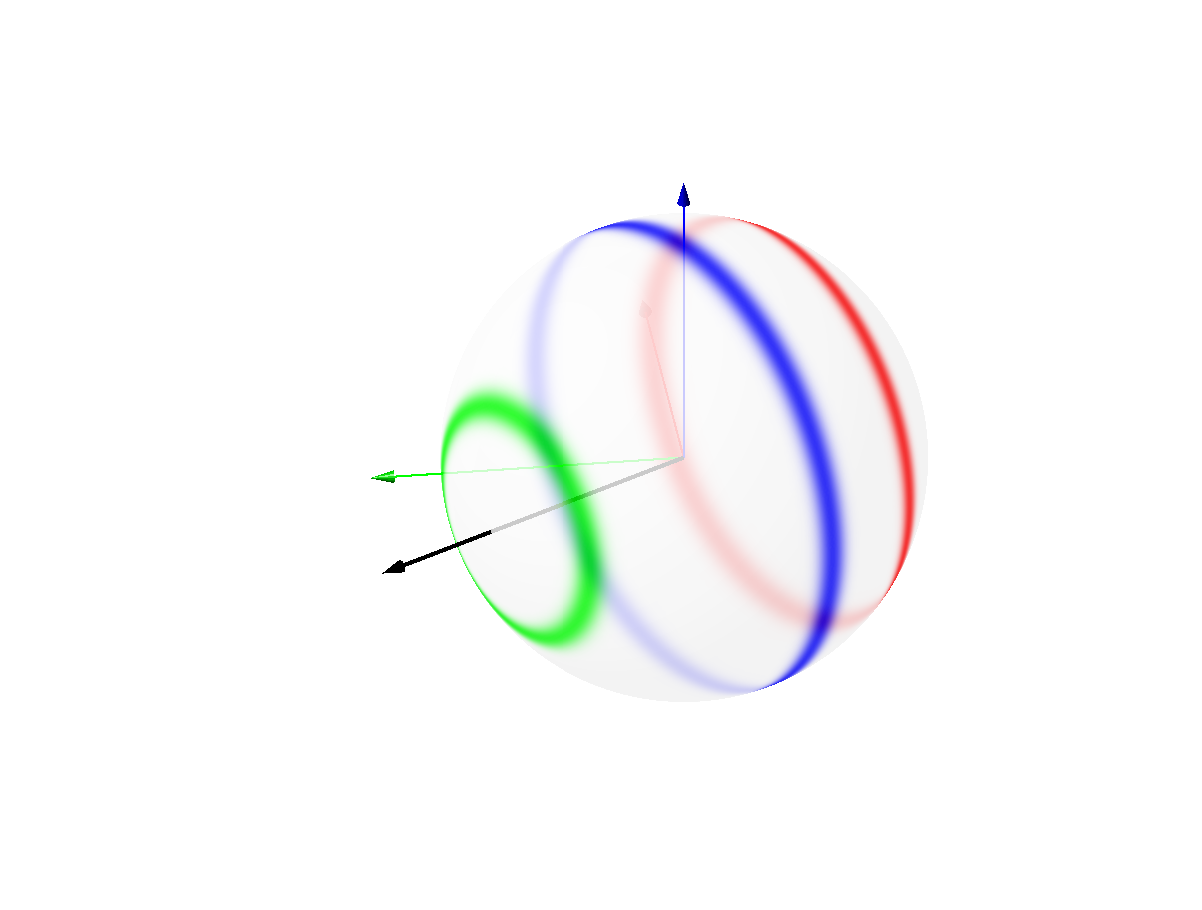
\includegraphics[trim=130 80 120 60, clip, scale=0.45]{figures/observability/mea_I_3}};
		
		\node at (2.7,0) {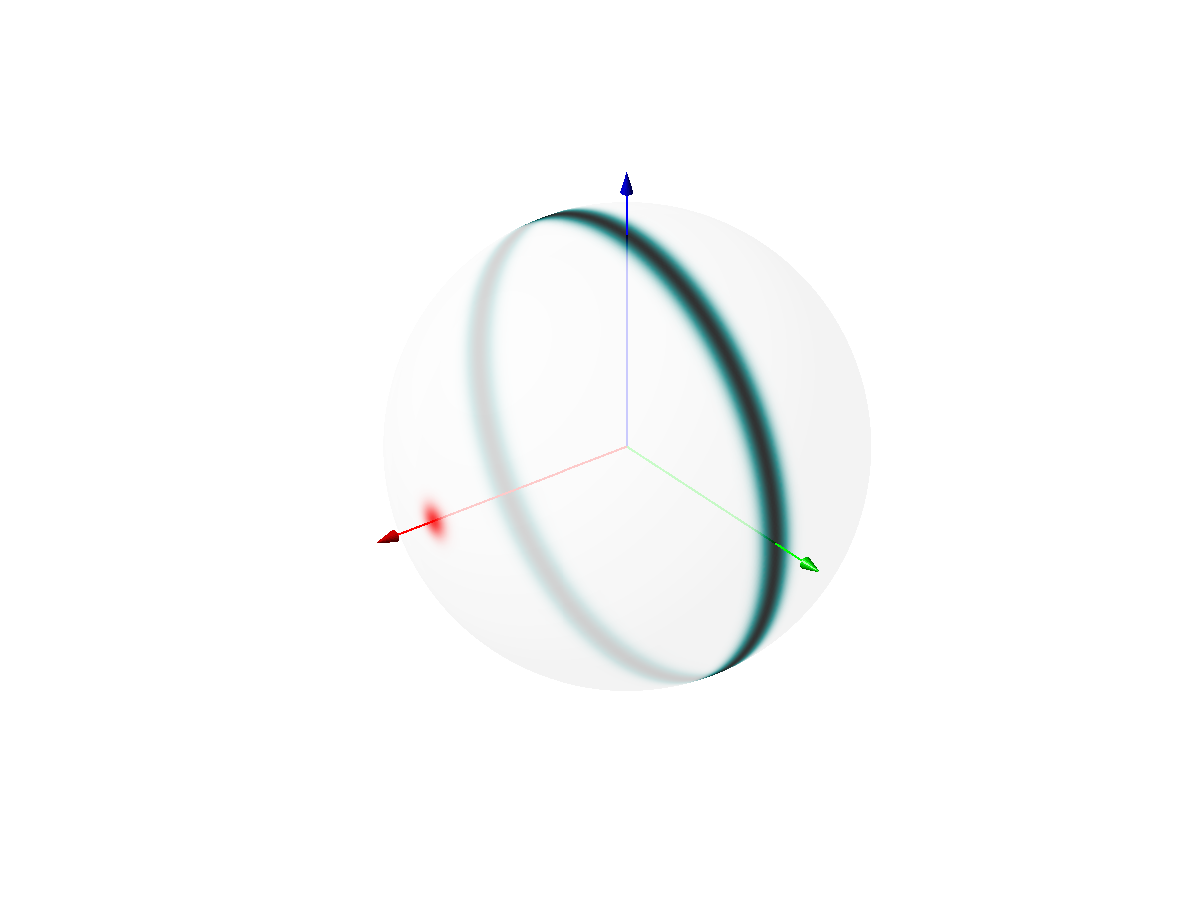
\includegraphics[trim=150 80 120 60, clip, scale=0.45]{figures/observability/mea_B_1}};
		\node at (7.8,0) {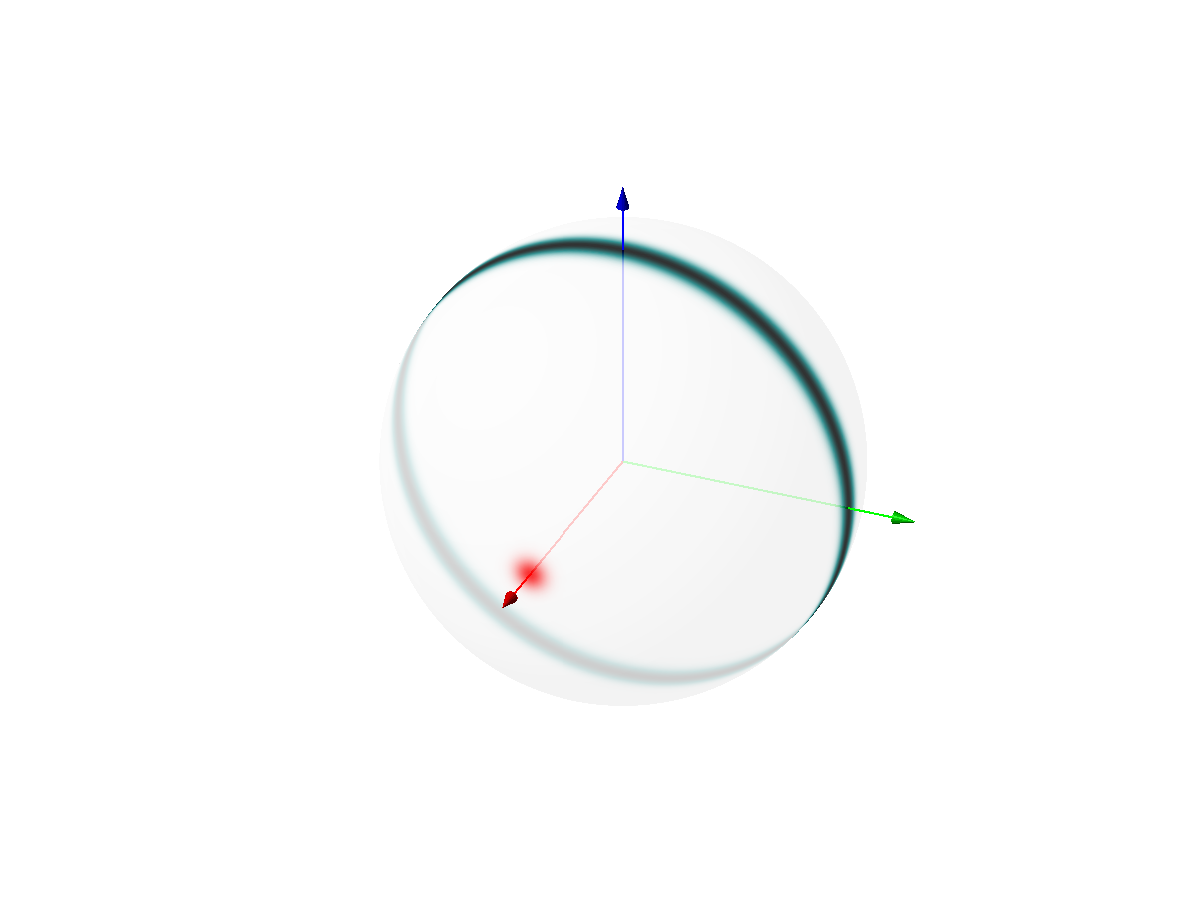
\includegraphics[trim=150 80 120 60, clip, scale=0.45]{figures/observability/mea_B_2}};
		\node at (12.8,0) {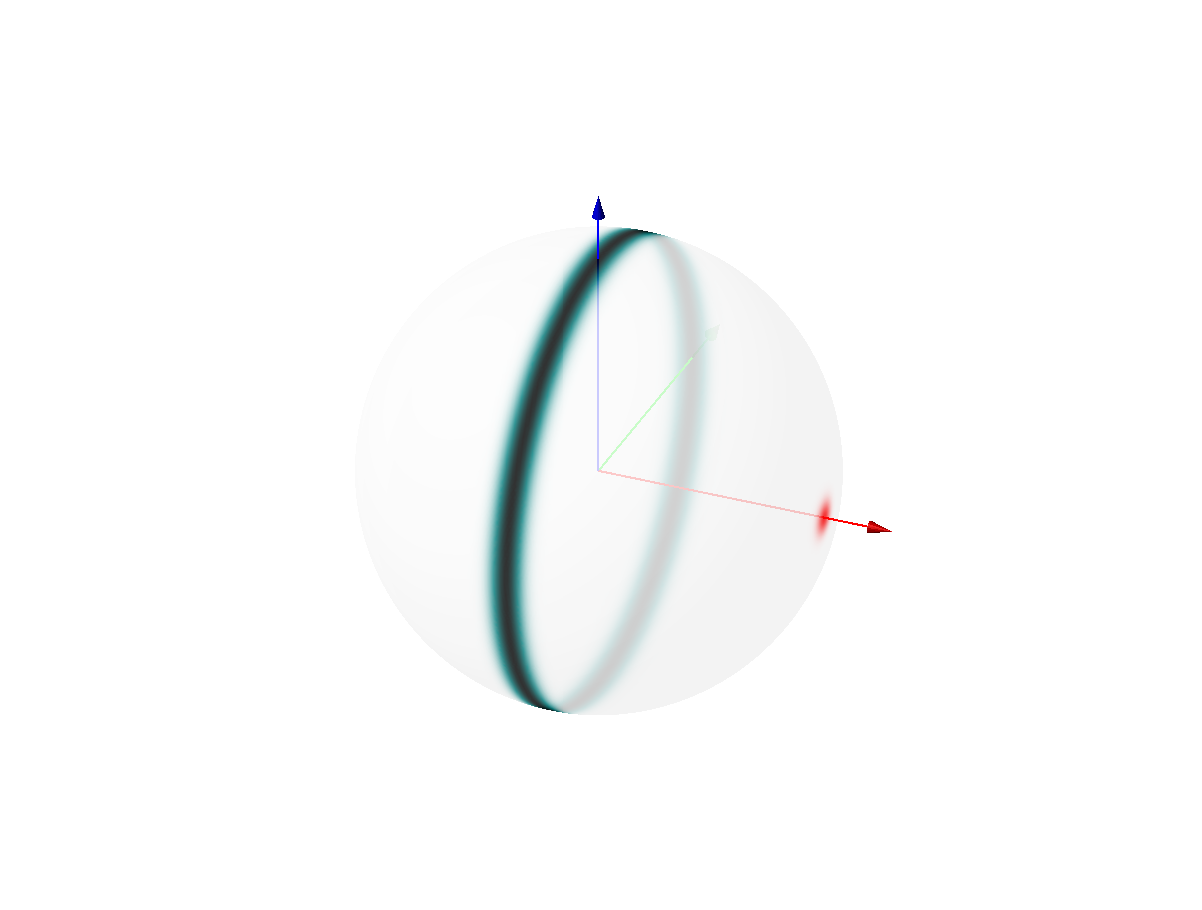
\includegraphics[trim=150 80 120 60, clip, scale=0.45]{figures/observability/mea_B_3}};
		
		\node at (0,5.5) {\rotatebox{90}{inertial dir. mea. \eqref{eqn:observability-measurement-inertial}}};
		\node at (0,0) {\rotatebox{90}{body-fixed dir. mea. \eqref{eqn:observability-measurement-body}}};
		
		\draw[arrows={-Triangle[angle=30:8pt]}] (5.25,-1.7) -- ++(90:0.8);
		\draw[arrows={-Triangle[angle=30:8pt]}] (5.25,-1.7) -- ++(-30:0.8);
		\draw[arrows={-Triangle[angle=30:8pt]}] (5.25,-1.7) -- ++(210:0.8);
		\node at (4.35,-2.1) {$\bm{e}_1$};
		\node at (6.25,-2.1) {$\bm{e}_2$};
		\node at (5.25,-0.7) {$\bm{e}_3$};
		
		\node at (0.8,7.2) {(a)};
		\node at (5.8,7.2) {(b)};
		\node at (10.8,7.2) {(c)};
		\node at (0.8,1.55) {(d)};
		\node at (5.8,1.55) {(e)};
		\node at (10.8,1.55) {(f)};
		
		\node at (2.8,2.6) {$x=e_1$};
		\node at (7.7,2.6) {$x=\tfrac{\sqrt{3}}{2}e_1 + \tfrac{1}{2}e_2$};
		\node at (12.6,2.6) {$x=-\tfrac{1}{2}e_1 + \tfrac{\sqrt{3}}{2}e_2$};
		
		\node at (2.8,-3.0) {$y=e_1$};
		\node at (7.7,-3.0) {$y=\tfrac{\sqrt{3}}{2}e_1 + \tfrac{1}{2}e_2$};
		\node at (12.6,-3.0) {$y=-\tfrac{1}{2}e_1 + \tfrac{\sqrt{3}}{2}e_2$};
	\end{tikzpicture}
	
	\caption[Posterior distribution with single direction measurements.]{Posterior distribution with single direction measurements ($\kappa=500$): (a-c) inertial direction measurements \eqref{eqn:observability-measurement-inertial} with $a=e_1$; (d-f) body-fixed direction measurements \eqref{eqn:observability-measurement-body} with $b=e_1$.}
	\label{fig:observability-measurement}
\end{figure}

Next, the implications of \eqref{eqn:observability-measurement-F_I} and \eqref{eqn:observability-measurement-F_B} are studied.
Suppose that the attitude is completely unknown before the measurement, i.e., $F^-=0_{3\times 3}$. 
For the inertial direction measurement, the matrix parameter \eqref{eqn:observability-measurement-F_I} for the posterior distribution is decomposed into
\begin{align} \label{eqn:observability-measurement-SVD_FI}
	F_I^+  = \begin{bmatrix} a & a' & a'' \end{bmatrix} 
	\diag(\kappa, 0,0) \begin{bmatrix} x & x' & x'' \end{bmatrix}^T,
\end{align}
where $a',a''\in\Sph^2$ are arbitrarily chosen such that the matrix $[a,a',a'']\in\SO{3}$, and $x',x''\in\Sph^2$ are defined similarly.
Therefore, $F_I^+$ is written in the form of pSVD with $S=\diag(\kappa,0,0)$. 
The first principal axis is $a$ when resolved in the inertial frame, or $x$ when resolved in the body-fixed frame. 
Also, the rotation about the first principal axis is completely unknown as $s_2+s_3 = 0$.
More intuitively, the marginal distribution of each body-fixed axis makes a circle normal to $\bm{a}$ (the top row of Figure \ref{fig:observability-measurement}), which implies the rotation about $\bm{a}$ cannot be determined.
Since $\bm{a}$ is fixed in the inertial frame, the direction of this ambiguity is also fixed in the inertial frame regardless of the measurement.

Next, the matrix parameter \eqref{eqn:observability-measurement-F_B} for the posterior distribution of a body-fixed direction measurement is decomposed into
\begin{align} \label{eqn:observability-measurement-SVD_FB}
	F_B^+  = \begin{bmatrix} y & y' & y'' \end{bmatrix} 
	\mathrm{diag}[\kappa, 0,0] \begin{bmatrix} b & b' & b'' \end{bmatrix}^T,
\end{align}
where $y',y''\in\Sph^2$ and $b',b''\in\Sph^2$ are chosen such that the corresponding matrices in brackets belong to $\SO{3}$. 
The resulting first principal axis is $b$ when resolved in the body-fixed frame, or $y$ when resolved in the inertial frame.
The marginal distribution of each body-fixed axis makes a circle normal to $\bm{b}$ (the bottom row of Figure \ref{fig:observability-measurement}), about which the rotation cannot be determined.
Since $\bm{b}$ is fixed in the body-fixed frame, the direction of this ambiguity is also fixed to the body.

\subsection{Stochastic Observability Criterion}

To formally study the attitude observability with single direction measurements, here two stochastic attitude observability criteria are introduced.
Since the posterior distribution of $R$ conditioned by measurements contains all the information available to determine the attitude, we study:
(i) whether there is a \textit{unique} attitude that minimizes the mean square error for the posterior distribution,
and (ii) whether the Fisher information matrix for the mean attitude of $R$ is positive-definite when $R$ is distributed according to the matrix Fisher distribution.

One of the methods to estimate an attitude from a density function on $\SO{3}$ is to solve an optimization problem that minimizes the mean square Frobenius norm.
\begin{definition}
	Let $p(R)$ be the probability density function for a random $R\in\SO{3}$. 
	Its minimum mean square estimate (MMSE) is defined as
	\begin{align}
		\mathrm{M}_{\mathrm{MMSE}} [R] = \argmin_{Q\in\SO{3}} \{\expect{\| R - Q\|_F^2 }\},
	\end{align}
	where $\|\cdot \|_F$ denotes the Frobenius norm.
\end{definition}

Finding MMSE can be addressed in terms of pSVD as follows.

\begin{lemma} \label{lemma:observability-MMSE}
	Suppose $R\in\SO{3}$ is a random rotation matrix.
	Let the pSVD of its first moment be $\expect{R}=UDV^T$ with $D=\mathrm{diag}[d_1,d_2,d_3]$. 
	Depending on $D$, the MMSE of $R$ is given by
	\begin{enumerate}
		\item $d_2+d_3 >0$: $UV^T$ (unique),
		\item $d_1\neq d_2$ and $d_2+d_3=0$: $\{U\exp(\theta\hat e_1) V^T\,|\,\theta\in[-\pi,\pi)\}$ (1D),
		\item $d_1=d_2 = -d_3 >0$: $\{U\exp(\theta\hat a) V^T|\, a\in\Sph^2,\; a_3 =0, \theta\in[-\pi,\pi)\}$ (2D),
		\item $d_1=d_2=d_3=0$:  $\SO{3}$ (3D),
	\end{enumerate}
	where the number in the parentheses indicates the dimension of the set corresponding to the solution of MMSE.
\end{lemma}
\begin{proof}
	The proof uses the equivalent definition \cite{lee2018bayesian}
	\begin{align*}
		\mathrm{M}_{\mathrm{MMSE}} [R] = \argmax_{R\in\SO{3}} \{\tr{R^T\expect{R}}\}.
	\end{align*}
	Let $\theta\in[-\pi,\pi)$ and $a\in\Sph^2$ be defined such that $U^T R V = \exp(\theta\hat a)$. 
	Then, it can be shown that
	\begin{align} \label{eqn:observability-trsRER}
		\tr{R^T \expect{R}} = \tr{D} - (1-\cos\theta) \sum_{i=1}^3 (d_i+d_j) a_k^2,
	\end{align}
	for $i\neq j\neq k$ and $i,j,k\in\{1,2,3\}$.
	Since $d_1+d_2 \geq d_3+d_1 \geq d_2 +d_3 \geq 0$, the above is maximized when $\theta=0$, or equivalently $R= UV^T$. 
	
	The uniqueness is contributed by two aspects: the uniqueness of $UV^T$ from the proper singular value decomposition and the uniqueness of the maximum at \eqref{eqn:observability-trsRER}.
	First note that the non-uniqueness of proper singular vectors caused by any simultaneous sign change of the corresponding columns of $U$ and $V$ does not affect the uniqueness of $UV^T$, therefore only the non-uniqueness of $U,V$ caused by repeated singular values is considered.
	\begin{enumerate}
		\item $d_2+d_3 >0$:
		If $d_3\geq 0$, the polar decomposition of $\expect{R}$ is written as $\expect{R} = (UV^T) \cdot (VDV^T)$, where $VDV^T = (\expect{R}^T\expect{R})^{1/2}$ is uniquely determined.
		The rank of $VDV^T$ is at least two, so $UV^T$ rotates two independent columns of $VDV^T$ to the corresponding columns of $\expect{R}$, and therefore it is unique.
		
		Next, when $d_3<0$, consider two sub-cases: (i) if $d_1\neq d_2$, then both $U$ and $V$ are unique; (ii) if $d_1=d_2$, $(U,V)$ can be replaced by $(U\exp(\phi\hat{e}_3),V\exp(\phi\hat{e}_3))$ for any $\phi\in[-\pi,\pi)$, but $UV^T$ is still unique.
		\item[2a)] $d_1 \neq d_2 =  d_3 =  0$:  It can be shown that
		\begin{align*}
			\tr{R^T \expect{R}} & = \tr{D} - (1-\cos\theta) d_1 (1-a_1^2),
		\end{align*}
		which is maximized for any $R$ in the given set of $a=e_1$. 
		The matrices $U$ and $V$ can be replaced with 
		$U\exp(\phi_1\hat e_1)$ and $V\exp(\phi_2\hat e_1)$, respectively, for any $\phi_1,\phi_2\in[-\pi,\pi)$. 
		However, the ambiguity of $U,V$ does not enlarge the set of $R$ maximizing \eqref{eqn:observability-trsRER}.
		\item[2b)] $d_1 \neq d_2 = -d_3 >0$: Similarly, \eqref{eqn:observability-trsRER} is maximized for any $R$ in the given set.
		The matrices $(U,V)$ can be replaced with 
		$(U\exp(\phi\hat e_1), V\exp(-\phi\hat e_1))$ for any $\phi\in[-\pi,\pi)$.
		But, it does not alter the given set. 
		\item[3)] $d_1 = d_2 = -d_3 >0$: It can be shown that
		\begin{align*}
			\tr{R^T \expect{R}} = \tr{D} - (1-\cos\theta)(d_1+d_2)a_3^2,
		\end{align*}
		which is maximized when $a_3=0$. 
		The ambiguity of $U$ and $V$ is written as $U\exp(\phi_1\hat e_1+\phi_2 \hat e_2 +\phi_3 \hat e_3)$ and $V\exp(-\phi_1\hat e_1 - \phi_2\hat e_2 +\phi_3\hat e_3)$, respectively for any $\phi_1,\phi_2,\phi_3\in[-\pi,\pi)$.
		Same as above, this does not alter the set of $R$ maximizing \eqref{eqn:observability-trsRER}.
		\item[4)] $d_1 = d_2=d_3=0$: This is a trivial case when $\tr{R^T \expect{R}}=0$ for any $R\in\SO{3}$.
	\end{enumerate}
	These complete the proof.
\end{proof}

For all cases, the set of MMSE contains $UV^T$.
Nevertheless, only when $d_2+d_3>0$, the MMSE is unique.
Otherwise, it can only be determined up to a rotation, where the dimension of the set representing the solution of MMSE is equivalent to 3 minus the rank of $\tr{D}I_{3\times 3}-D = \diag(d_2+d_3, d_1+d_3, d_1+d_2)$.
Therefore, it is claimed that the attitude is completely observable given a density function on $\SO{3}$ if $\tr{D}I_{3\times 3}-D$ is positive-definite, i.e., when the MMSE is unique.

The above observability criterion is solely based on the first moment, and therefore, it can be applied to an unknown attitude following an arbitrary distribution. 
Next, it is assumed that the attitude is distributed according to a matrix Fisher distribution to present an alternative information theoretic observability criterion.

Suppose $R\sim \mathcal{M}(F)$ where the pSVD of $F\in\mathbb{R}^{3\times 3}$ is given by $F=USV^T$.
As discussed in Chapter \ref{section:MF-MF}, the MMSE of $R\sim\mathcal{M}(USV^T)$ is given by the mean attitude $R^*=UV^T$, and we want to calculate its Fisher information $\mathbb{I}(R^*)$.
To do this, first a more general problem of estimating $U$, $S$, and $V$ from the given samples of $R$ is studied.
The log-likelihood is
\begin{align} \label{eqn:observability-FIM-likelihood}
	l(R|U,S,V) = \tr{USV^T R^T} - \log c(S).
\end{align}
And the corresponding Fisher information matrix is calculated as follows~\cite{smith2005covariance}.

\begin{lemma} \label{lemma:observability-FIM}
	The Fisher information matrix of \eqref{eqn:observability-FIM-likelihood}, namely $\mathbb{I}(U,S,V): \SO{3} \times \mathbb{R}^3 \times \SO{3} \rightarrow \mathbb{R}^{9\times 9}$ is constructed as 
	\begin{align} \label{eqn:observability-FIM}
		\mathbb{I} (U,S,V) &= -\expect{ \nabla^2 l (R|U,S,V) }\nonumber \\
		&=\begin{bmatrix}
			\tr{DS}I_{3\times 3}- DS  & 0 & \sum_{i=1}^3 e_i^T s \hat e_i D\hat e_i \\
			0 & \frac{\partial^2 \log c(S)}{\partial s^2} & 0 \\
			\sum_{i=1}^3 e_i^T s \hat e_i D\hat e_i& 0 & \tr{DS}I_{3\times 3} -DS
		\end{bmatrix},
	\end{align}
	where $D\in\mathbb{R}^{3\times 3}$ is the diagonal matrix composed of the proper singular values of $\expect{R|U,S,V}$, $S = \diag(s_1, s_2, s_3)$, and $\nabla^2$ is the covariant Hessian on $\SO{3}\times\mathbb{R}^3\times\SO{3}$.
\end{lemma}
\begin{proof}
	Let $\mathsf{Q} = \SO{3}\times\mathbb{R}^3\times\SO{3}$, and $q=(U,S,V)\in\mathsf{Q}$.
	The tangent space $\mathsf{T}_q\mathsf{Q}$ is identified with $\mathsf{T}_q\mathsf{Q}\simeq \mathbb{R}^9$ through the hat map, and the cotangent space is also identified with $\mathbb{R}^9$ using the dot product.
	More specifically, for $\xi=(u,\varsigma,v)\in\mathbb{R}^9$, the corresponding tangent vector is given by $(U\hat u, \varsigma, V\hat v)\in\mathsf{T}_q \mathsf{Q}$. 
	
	Since $l$ is a real-valued function on $\mathsf{Q}$, its covariant derivative $\nabla_\xi l$ along $\xi$ is equivalent to the differential $dl(\xi)$ given by
	\begin{align*}
		&\nabla_\xi l = \frac{d}{d\epsilon}\bigg|_{\epsilon =0} l( R | U\exp(\epsilon\hat u), S+\epsilon\mathrm{diag}[\varsigma], V\exp(\epsilon\hat v))\\
		& = \tr{(U\hat uSV^T + U\mathrm{diag}[\varsigma]V^T - US\hat v V^T)^TR} - \frac{\partial \log c(S)}{\partial s}\cdot \varsigma \\
		& = 
		\begin{bmatrix}
			(QS-SQ^T)^\vee \\ 
			\mathrm{diag}[Q]-\frac{1}{c(S)} \frac{\partial c(S)}{\partial s} \\
			(Q^TS - SQ)^\vee
		\end{bmatrix}\cdot \xi,
	\end{align*}
	where $Q=U^TRV$.
	Because $\expect{Q} = D$ is diagonal, it is straightforward to show $\expect{dl(\xi)}=0$ for any $\xi\in\mathbb{R}^9$.
	
	The covariant Hessian of $l$ along $\xi_1$ and $\xi_2$ is given by $\nabla^2_{\xi_1,\xi_2} l = \xi_2(\xi_1 l) - (\nabla_{\xi_2}\xi_1) l = \xi_2 ( dl(\xi_1)) - dl(\nabla_{\xi_2} \xi_1)$,
	where the second term vanishes after taking expectation.
	The first term is bi-linear in $\xi_1$ and $\xi_2$, thus it can be written as a matrix as in \eqref{eqn:observability-FIM}.
	Suppose $\xi_1 = (u_1,0,0)$ and $\xi_2 =(u_2,0,0)$, then it can be shown that
	\begin{align*}
		\xi_2 (dl(\xi_1)) = (-\hat u_2 QS -SQ^T \hat u_2)^\vee \cdot u_1 = u_1^T \left\{\frac{1}{2}(QS+SQ^T) - \tr{QS}I_{3\times 3}\right\} u_2.
	\end{align*}
	Taking the expectation of the expression in the braces with $\expect{Q}=D$ and multiplying it with $-1$ yield the upper-left 3-by-3 block of \eqref{eqn:observability-FIM}.
	The remaining blocks can be obtained similarly.
\end{proof}

Next, the Fisher information $\mathbb{I}(R^*)$ can be obtained with the above information matrix.
Since the variations of $U$ and $V$ are written as $\delta U = U\hat u$ and $\delta V= V\hat v$ for $u,v\in\mathbb{R}^3$, it can be shown that
\begin{align*}
	\delta R^* = U\hat u V^T - U\hat vV^T.
\end{align*}
Let $\eta = u-v\in\mathbb{R}^3$ so that $\delta R^* = U\hat\eta V^T$.
Thus, the Fisher information matrix for the mean attitude $R^*$ is constructed by left-multiplying \eqref{eqn:observability-FIM} with the matrix $\frac{1}{2} [I_{3\times 3}; 0_{3\times 3}; -I_{3\times 3}]$, and by right-multiplying \eqref{eqn:observability-FIM} with its transpose, to obtain
\begin{align}
	\mathbb{I}(R^*) = \frac{1}{2} \mathrm{diag} \!
	\begin{bmatrix} (d_2+d_3)(s_2+s_3) \\ (d_3+d_1)(s_3+s_1) \\ (d_1+d_2)(s_1+s_2) \end{bmatrix}.\label{eqn:FIM_eta}
\end{align}
According to the Cram\'{e}r--Rao inequality, the inverse of Fisher information $\mathbb{I}(R^*)$ is a lower bound of the variance of all unbiased estimates, up to additional curvature terms.
Therefore, its positive-definiteness can be used to define observability \cite{mohler1988nonlinear}.
Interestingly, by Lemma \ref{lemma:MF-SD}, the positive-definiteness of $\mathbb{I}(R^*)$ is equivalent to the uniqueness of MMSE presented in Lemma \ref{lemma:observability-MMSE}.
Based on these results, we formulate stochastic attitude observability for an arbitrary density as follows.
\begin{definition} \label{def:observability}
	A random rotation matrix $R\sim p(R)$ is stochastically observable if $d_2+ d_3 >0$, or equivalently
	\begin{align}
		\mathcal{O} = \tr{D}I_{3\times 3} - D \succ 0,\label{eqn:OC}
	\end{align}
	where $D=\mathrm{diag}[d_1,d_2,d_3]$ is the proper singular values of $\expect{R}$.  
	The corresponding measure of observability is
	\begin{align}
		\rho(R) = \det[\mathcal{O}] = (d_1+d_2)(d_3+d_1)(d_2+d_3).
	\end{align}
\end{definition}
When $R\sim\mathcal{M}(USV^T)$, it is straightforward to show that \eqref{eqn:OC} is equivalent to $\tr{S}I_{3\times 3} - S\succ 0$ with Lemma \ref{lemma:MF-SD}.
Note that these are readily applied to the stochastic observability considered in this section, as the posterior distribution conditioned by direction measurements is assumed to be a matrix Fisher distribution according to Theorem \ref{thm:F_post}, which is presented in the next subsection.

\subsection{Attitude Observability Results}

The attitude uncertainty propagation in Chapter \ref{section:observability-propagation}, and the measurement update in Chapter \ref{section:observability-measurement} constitute a Bayesian estimator, which provides the posterior distribution of the attitude conditioned by the history of direction measurements.
The posterior distribution can then be used in Definition \ref{def:observability} to determine attitude observability.
As there are two cases for each of uncertainty propagation and measurement update, there are four possible combinations as summarized in Table \ref{table:observability}.
This subsection identifies two combinations that yield unobservability, and two other cases resulting in observability with single direction measurements.
The same results can also be derived in a deterministic sense as presented in Appendix \ref{app:obervability-deterministic}.

We first discuss why the common IMU cannot estimate the full attitude with single direction measurements.
In a typical IMU, the angular velocity is measured in the body-fixed frame using a gyroscope, and the reference direction in the inertial frame, such as the direction of gravity, is measured in the body-fixed frame. 
As such it is a combination of the left-trivialized \eqref{eqn:observability-kinematics-left-dist} and the inertial direction measurement \eqref{eqn:observability-measurement-inertial}.
Looking at the bottom row of Figure \ref{fig:observability-kinematics} and the top row of Figure \ref{fig:observability-measurement}, it is clear why the attitude cannot be determined in this case: the direction about which the rotation cannot be determined, namely the first principal axis, remains unchanged in the inertial frame for both \eqref{eqn:observability-kinematics-left-dist} and \eqref{eqn:observability-measurement-inertial}.
This is formulated in the next theorem.

\begin{theorem} \label{thm:observability-nonobs}
	Consider the two Bayesian attitude estimators for
	\begin{itemize}
		\item right-trivialized angular velocity in the inertial frame \eqref{eqn:observability-kinematics-right-dist} and body-fixed direction measurement \eqref{eqn:observability-measurement-body}  
		\item left-trivialized angular velocity in the body-fixed frame \eqref{eqn:observability-kinematics-left-dist}, and inertial direction measurement \eqref{eqn:observability-measurement-inertial} 
	\end{itemize}
	with the initial distribution $F_0=0_{3\times 3}$.
	For both cases, the attitude is not observable.
\end{theorem}
\begin{proof}
	First consider the filter given by \eqref{eqn:observability-kinematics-UV_R}, \eqref{eqn:observability-kinematics-S}, and \eqref{eqn:observability-measurement-F_B}.
	The propagated uncertainty before the first measurement is $F_1^- = 0_{3\times 3}$, thus $F_1 = \kappa y_1b^T$ after conditioning the first measurement.
	As shown in \eqref{eqn:observability-measurement-SVD_FB}, $(s_2)_1=(s_3)_1=0$, and $V_1e_1 = b$.
	We proceed with induction.
	Suppose $(s_2)_k=(s_3)_k=0$, and $V_ke_1 = b$.
	Then by \eqref{eqn:observability-kinematics-UV_R}, \eqref{eqn:observability-kinematics-S} and Lemma \ref{lemma:MF-SD}, the propagated parameters before the next measurement still satisfy $(s_2)_{k+1}^-=(s_3)_{k+1}^- = 0$ and $V_{k+1}^-e_1=b$.
	Next consider the update $F_{k+1} = F_{k+1}^-+\kappa y_{k+1}b^T$, which can be written as
	\begin{align*}
		F_{k+1} = \left((s_1)_{k+1}^-U_{k+1}^-e_1 + \kappa y_{k+1}\right)b^T \triangleq ub^T,
	\end{align*}
	where $u\in\mathbb{R}^3$.
	Let $U_{k+1} = \Big[ \frac{u}{\norm{u}}, u', u'' \Big]$, where $u',u''\in\Sph^2$ are arbitrarily chosen such that $U_{k+1}\in\SO{3}$.
	Also let $S_{k+1} = \diag(\norm{u},0,0)$, and $V_{k+1} = [ b, b', b'' ]$ as in \eqref{eqn:observability-measurement-SVD_FB}.
	Then $F_{k+1} = U_{k+1}S_{k+1}V_{k+1}^T = ub^T $ is the pSVD of $F_{k+1}$, and it has been shown that $(s_2)_{k+1}=(s_3)_{k+1}=0$ and $V_{k+1}e_1=b$.
	Therefore, $(s_2)_k=(s_3)_k=0$ for all $k\in\mathbb{N}$, and by Lemma \ref{lemma:MF-SD}, the attitude is not observable.
	The proof for the second case is similar.
\end{proof}

Next, two examples illustrating that the other two combinations yield observability are presented.
Consider the combination of right-trivialized \eqref{eqn:observability-kinematics-right-dist} and inertial direction measurement \eqref{eqn:observability-measurement-inertial} for a specific case where the true attitude evolves according to
\begin{align}
	R(t) = R_0 \exp(\hat\Omega t) = \exp(\hat\omega t) R_0,\label{eqn:R_est}
\end{align}
with $R_0=I_{3\times 3}$ and $\Omega = \omega = -\frac{\pi}{2\sqrt{3}}[1, 1, 1]\in\mathbb{R}^3$. 
Initially, it is assumed that the attitude is completely unknown, i.e., $F_0 = 0_{3\times 3}$, as illustrated in Figure \ref{fig:observability-est_RI}(a).
Then after updated by an inertial direction measurement with $a = e_1$, the rotation about the reference direction is unobservable and the resulting distribution is axially symmetric about $\mathbf{e}_1$ (Figure \ref{fig:observability-est_RI}(b)).
For the right-trivialized \eqref{eqn:observability-kinematics-right-dist}, the distribution rotates in the inertial frame over the propagation, and therefore, the direction of ambiguity is no longer along $\bm{e}_1$ (Figure \ref{fig:observability-est_RI}(c)(d)).
The next inertial direction measurement is fixed in the inertial frame along $\bm{e}_1$ (Figure \ref{fig:observability-est_RI}(e)).
Thus, it resolves the ambiguity of the propagated density to determine the attitude completely (Figure \ref{fig:observability-est_RI}(f)).

The other combination of left-trivialized \eqref{eqn:observability-kinematics-left-dist} and body-fixed direction measurement \eqref{eqn:observability-measurement-body} is similar.
The direction of ambiguity caused by the first body-fixed direction measurement with $b=e_1$ is fixed in the inertial frame after propagation (Figure  \ref{fig:observability-est_LB}(b)-(d)).
However, the ambiguous direction of the next direction measurement is rotated in the inertial frame (Figure \ref{fig:observability-est_LB}(e)), and this resolves the previous ambiguity (Figure \ref{fig:observability-est_LB}(f)).
The above intuition is formally presented in the next theorem.

\begin{figure}
	\centering
	\begin{tikzpicture}
		\node at (2.5,5.5) {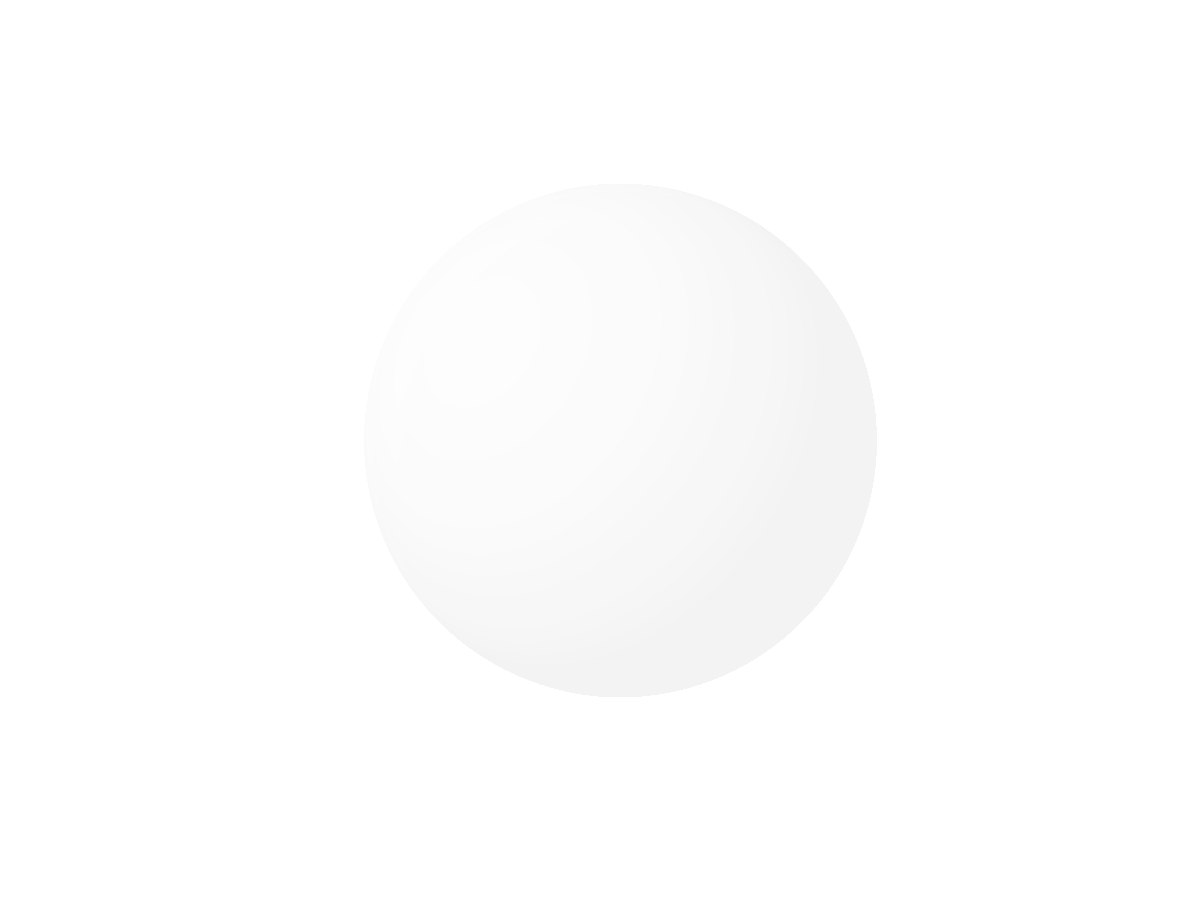
\includegraphics[trim=150 80 120 60, clip, scale=0.45]{figures/observability/est_RI_F1_prior}};
		\node at (7.5,5.5) {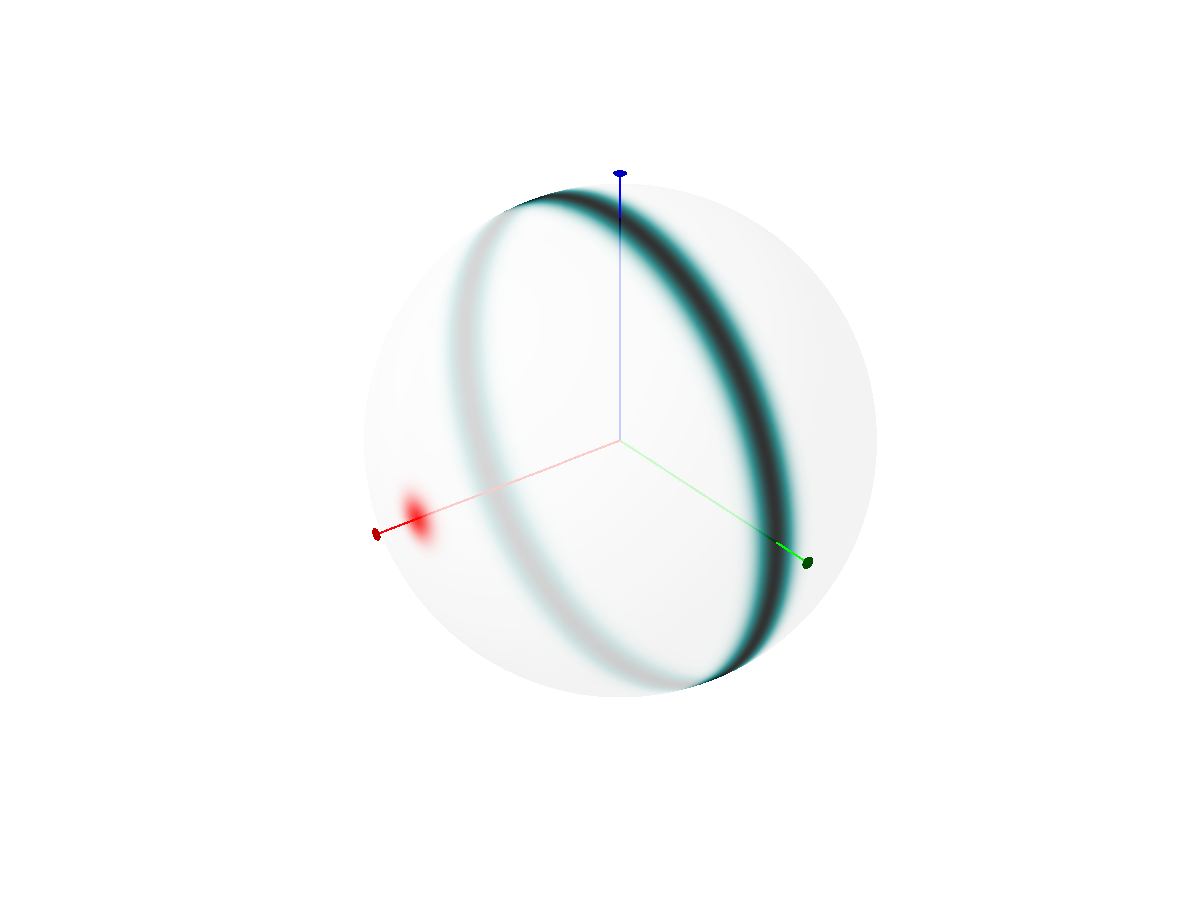
\includegraphics[trim=150 80 120 60, clip, scale=0.45]{figures/observability/est_RI_F1}};
		\node at (12.5,5.5) {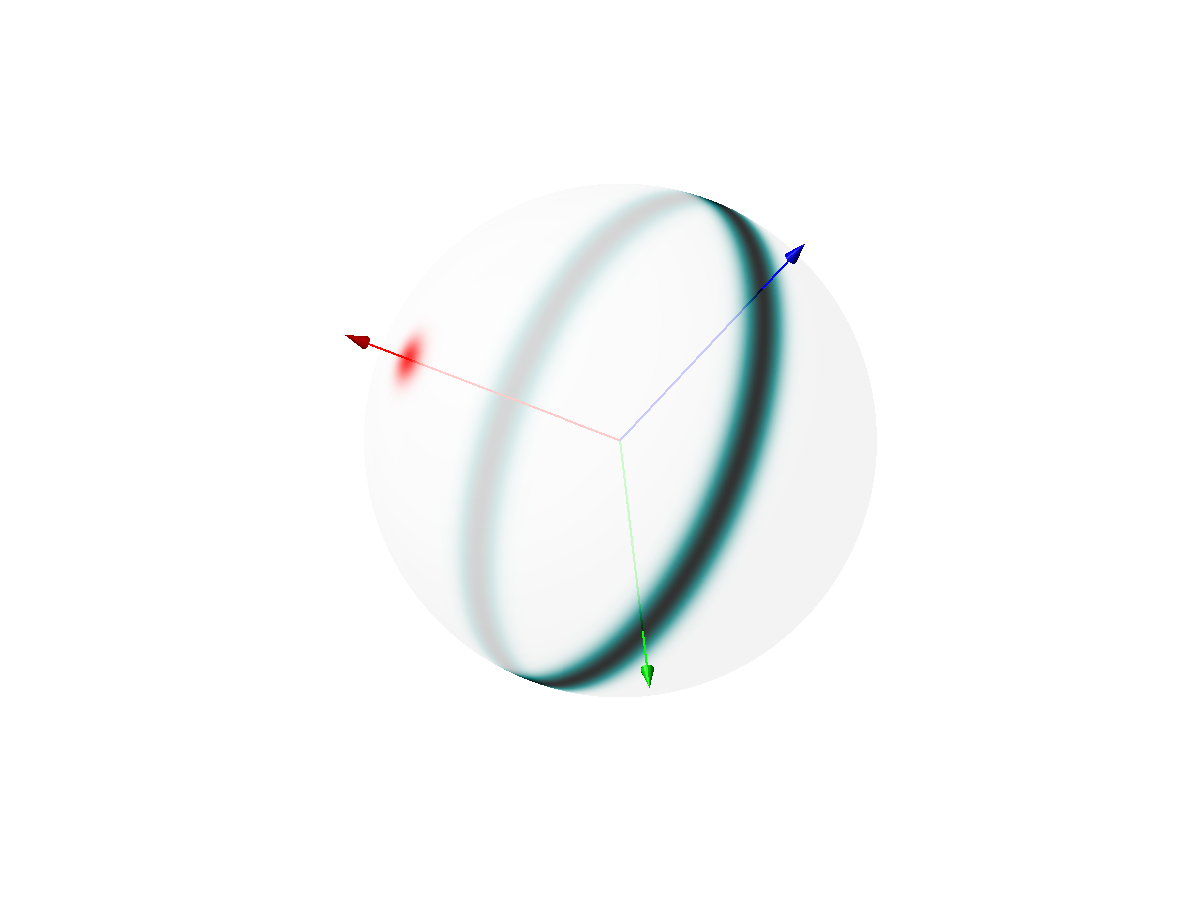
\includegraphics[trim=150 80 120 60, clip, scale=0.45]{figures/observability/est_RI_F3}};
		
		\node at (2.5,0) {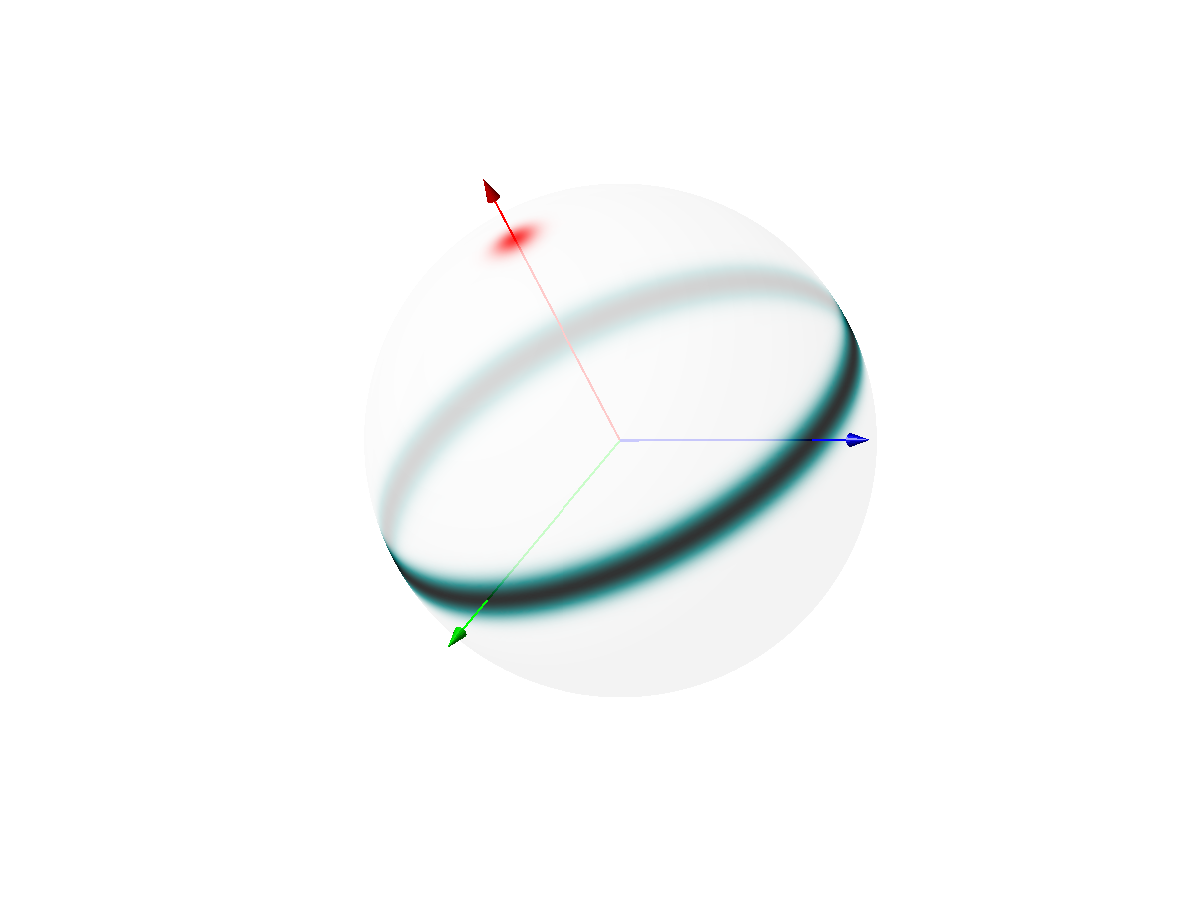
\includegraphics[trim=150 80 120 60, clip, scale=0.45]{figures/observability/est_RI_F5}};
		\node at (7.5,0) {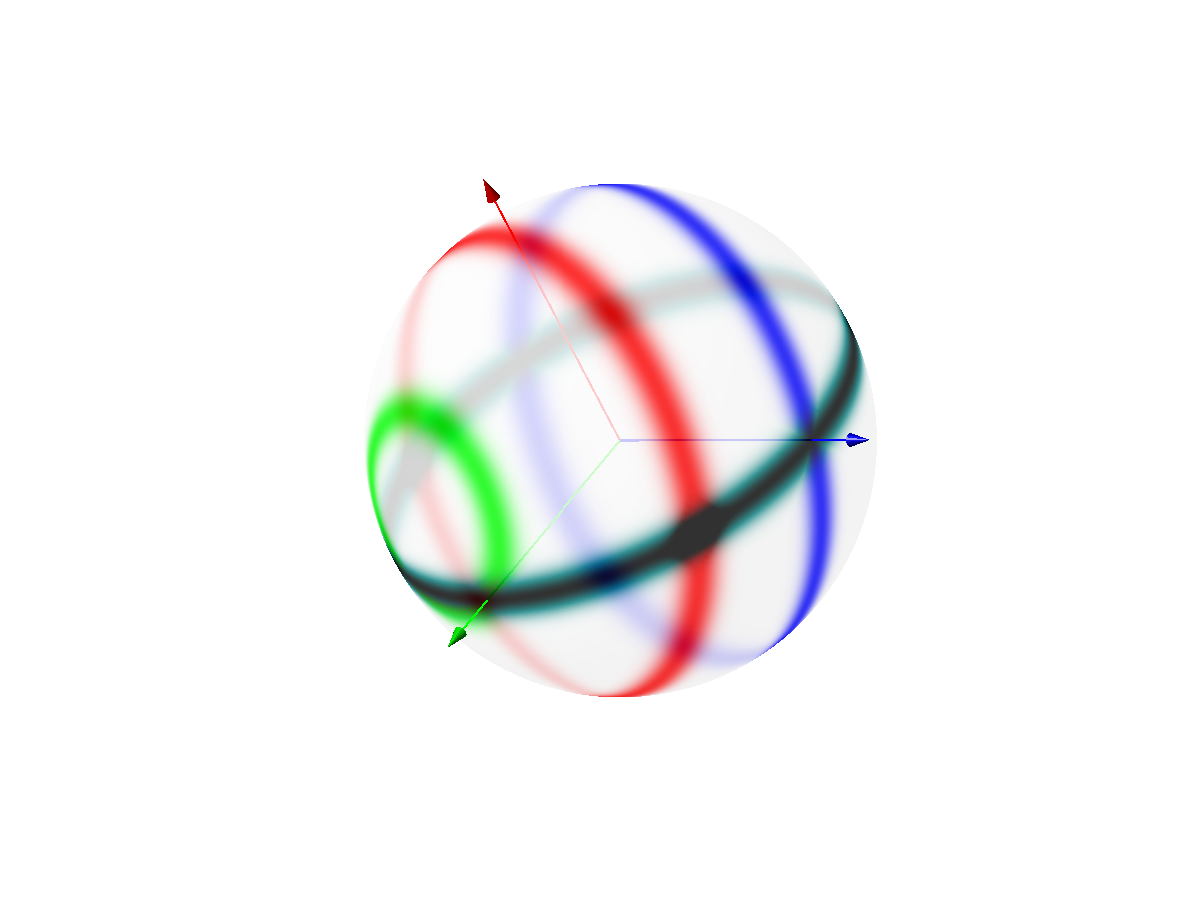
\includegraphics[trim=150 80 120 60, clip, scale=0.45]{figures/observability/est_RI_FN_mea}};
		\node at (12.5,0) {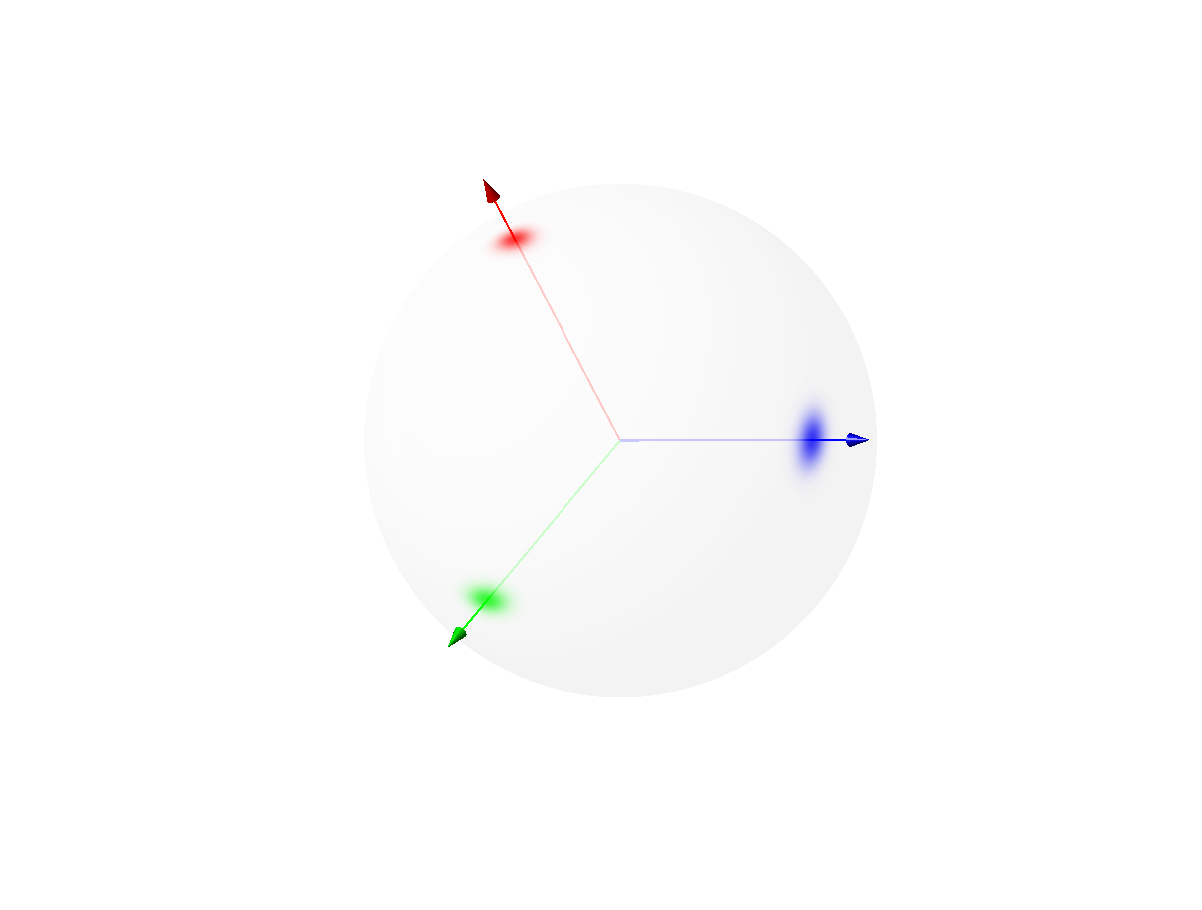
\includegraphics[trim=150 80 120 60, clip, scale=0.45]{figures/observability/est_RI_FN_post}};
		
		\draw[arrows={-Triangle[angle=30:8pt]}] (4.95,3.8) -- ++(90:0.8);
		\draw[arrows={-Triangle[angle=30:8pt]}] (4.95,3.8) -- ++(-30:0.8);
		\draw[arrows={-Triangle[angle=30:8pt]}] (4.95,3.8) -- ++(210:0.8);
		\node at (4.05,3.4) {$\bm{e}_1$};
		\node at (5.95,3.4) {$\bm{e}_2$};
		\node at (4.95,4.8) {$\bm{e}_3$};
		
		\node at (0.5,7.2) {(a)};
		\node at (5.5,7.2) {(b)};
		\node at (10.5,7.2) {(c)};
		\node at (0.5,1.55) {(d)};
		\node at (5.5,1.55) {(e)};
		\node at (10.5,1.55) {(f)};
		
		\node at (2.6,2.6) {Prior dist. at $t=0$};
		\node at (7.7,2.6) {Posterior dist. at $t=0$};
		\node at (12.6,2.6) {Propagated dist. at $t=0.5$};
		
		\node at (2.6,-3.0) {Propagated dist. at $t=1$};
		\node[align=center] at (7.7,-3.0) {Propagated dist. overlapped \\ with measured dist. at $t=1$};
		\node at (12.6,-3.0) {Posterior dist. at $t=1$};
	\end{tikzpicture}
	
	\caption[Estimation with the right trivialized \eqref{eqn:observability-kinematics-right-dist} and the inertial direction measurement \eqref{eqn:observability-measurement-inertial}.]{Estimation with the right trivialized \eqref{eqn:observability-kinematics-right-dist} and the inertial direction measurement \eqref{eqn:observability-measurement-inertial}, where the complete attitude is estimated after incorporating two inertial single direction measurements.}
	\label{fig:observability-est_RI}
\end{figure}

\begin{figure}
	\centering
	\begin{tikzpicture}
		\node at (2.5,5.5) {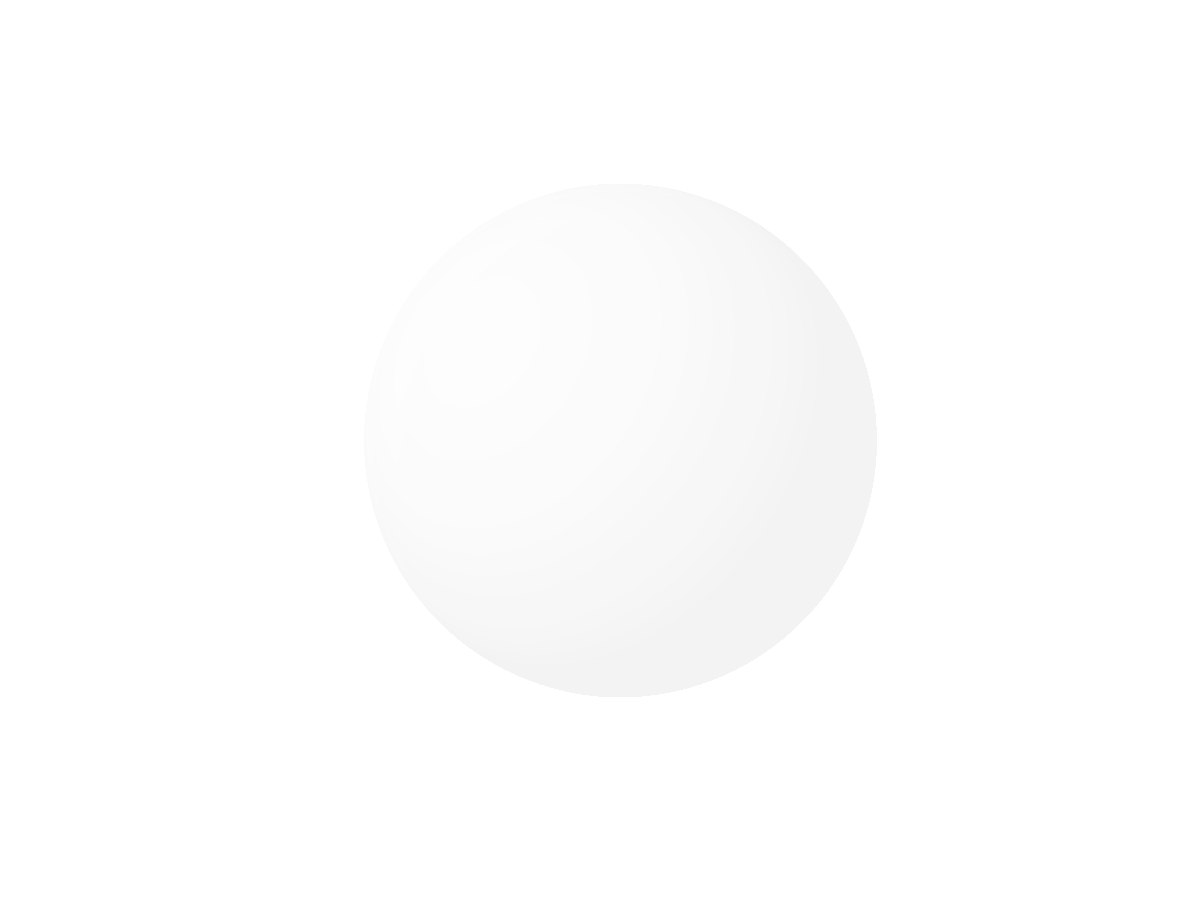
\includegraphics[trim=150 80 120 60, clip, scale=0.45]{figures/observability/est_LB_F1_prior}};
		\node at (7.5,5.5) {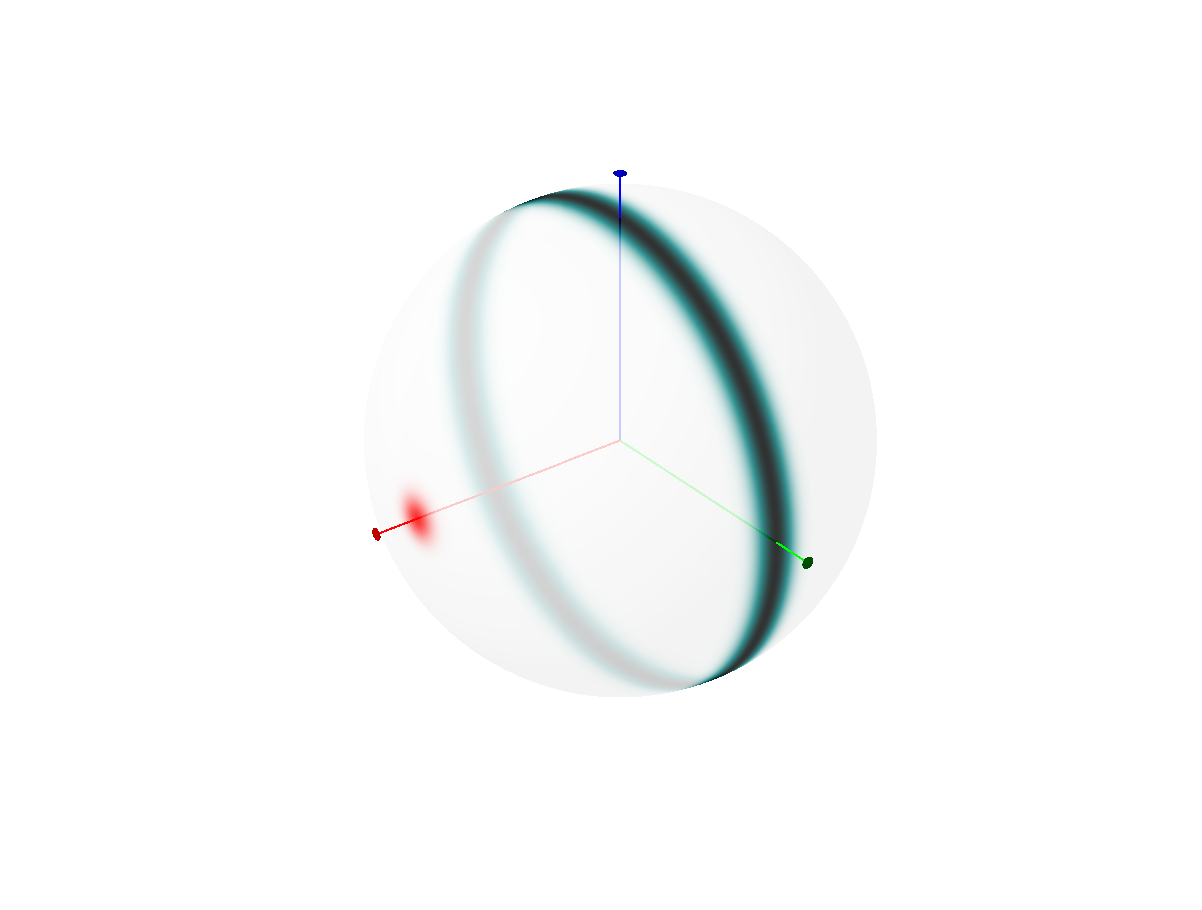
\includegraphics[trim=150 80 120 60, clip, scale=0.45]{figures/observability/est_LB_F1}};
		\node at (12.5,5.5) {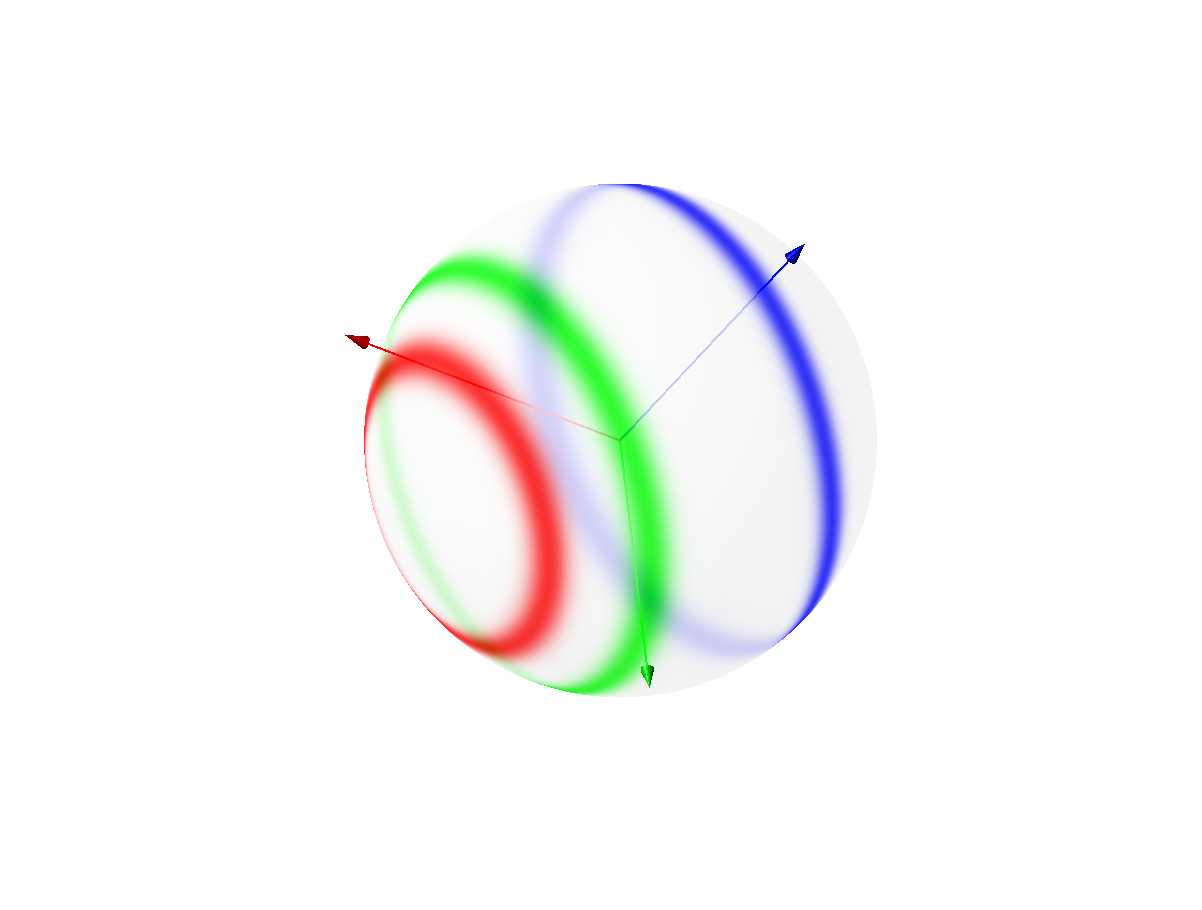
\includegraphics[trim=150 80 120 60, clip, scale=0.45]{figures/observability/est_LB_F3}};
		
		\node at (2.5,0) {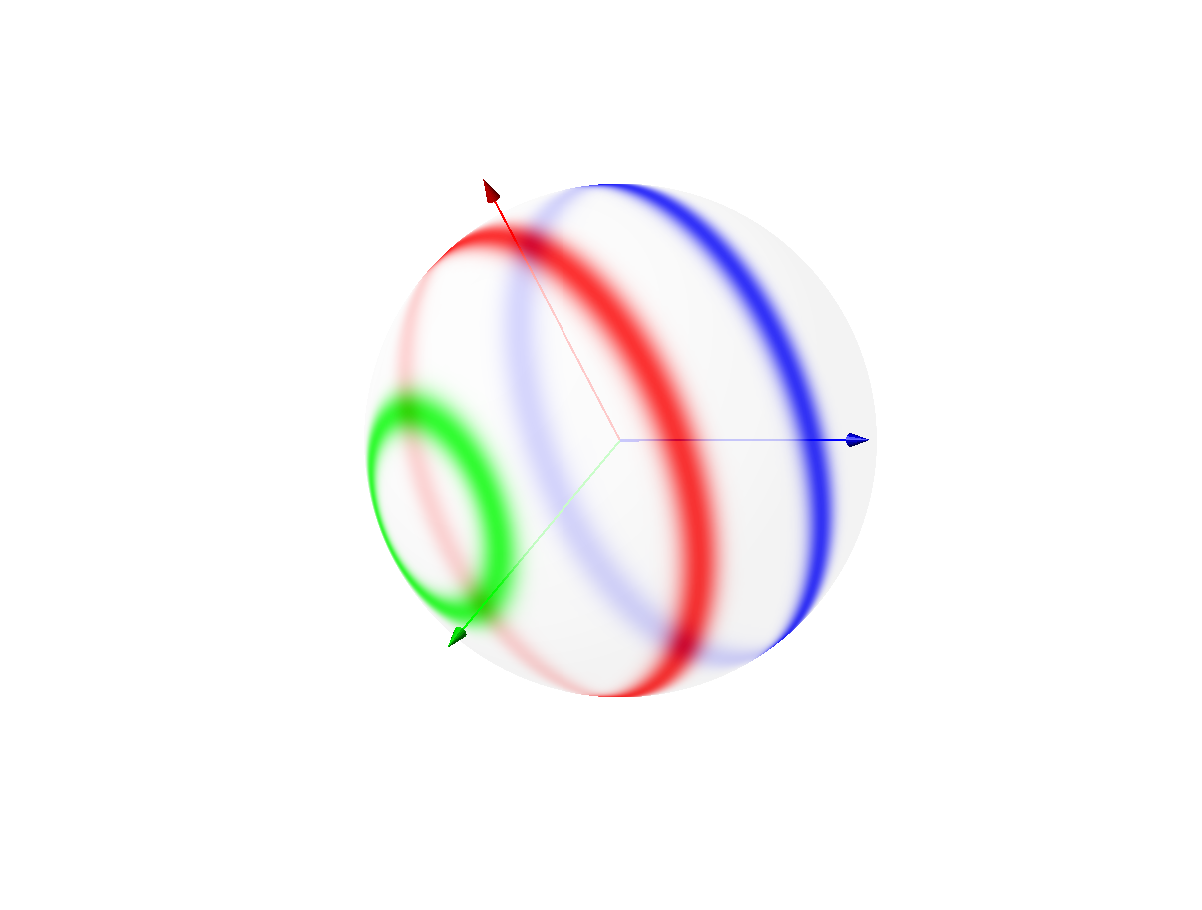
\includegraphics[trim=150 80 120 60, clip, scale=0.45]{figures/observability/est_LB_F5}};
		\node at (7.5,0) {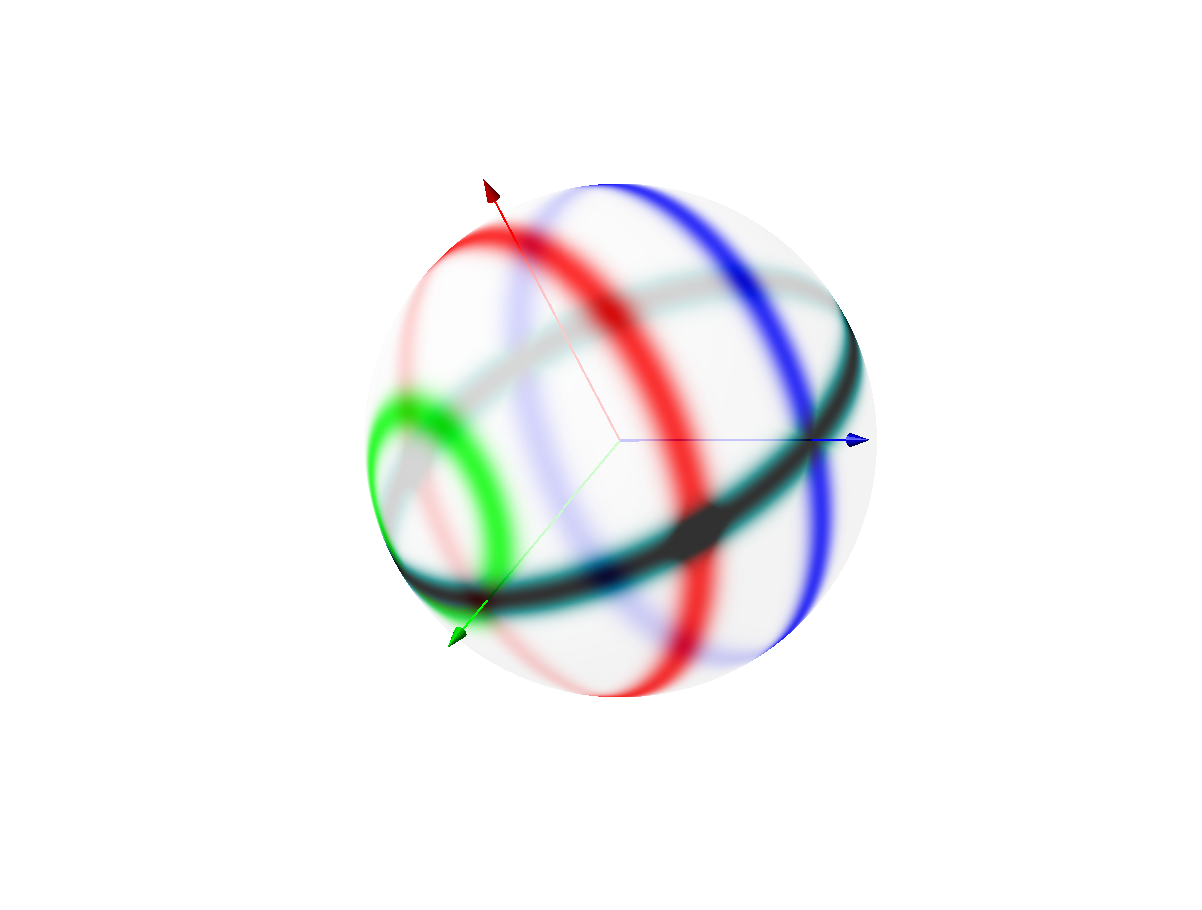
\includegraphics[trim=150 80 120 60, clip, scale=0.45]{figures/observability/est_LB_FN_mea}};
		\node at (12.5,0) {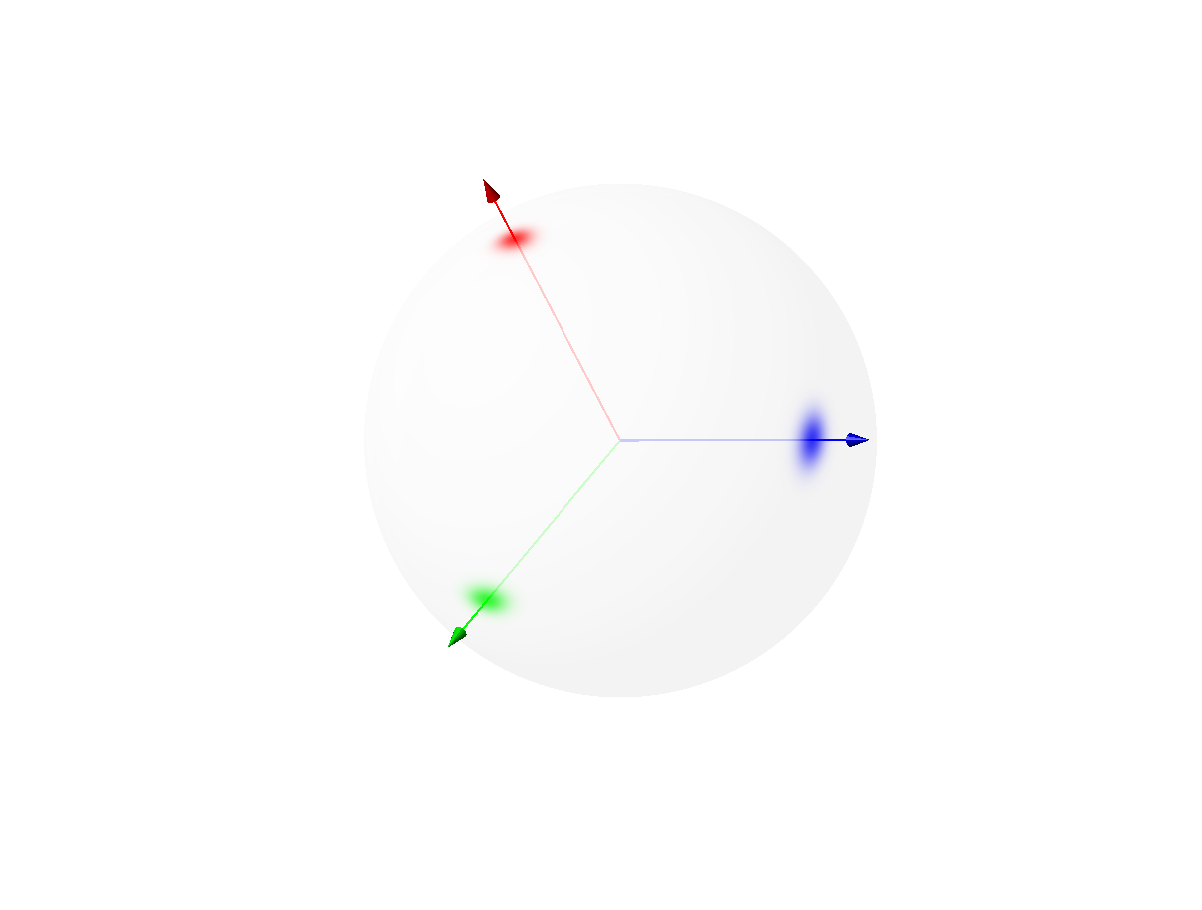
\includegraphics[trim=150 80 120 60, clip, scale=0.45]{figures/observability/est_LB_FN_post}};
		
		\draw[arrows={-Triangle[angle=30:8pt]}] (4.95,3.8) -- ++(90:0.8);
		\draw[arrows={-Triangle[angle=30:8pt]}] (4.95,3.8) -- ++(-30:0.8);
		\draw[arrows={-Triangle[angle=30:8pt]}] (4.95,3.8) -- ++(210:0.8);
		\node at (4.05,3.4) {$\bm{e}_1$};
		\node at (5.95,3.4) {$\bm{e}_2$};
		\node at (4.95,4.8) {$\bm{e}_3$};
		
		\node at (0.5,7.2) {(a)};
		\node at (5.5,7.2) {(b)};
		\node at (10.5,7.2) {(c)};
		\node at (0.5,1.55) {(d)};
		\node at (5.5,1.55) {(e)};
		\node at (10.5,1.55) {(f)};
		
		\node at (2.6,2.6) {Prior dist. at $t=0$};
		\node at (7.7,2.6) {Posterior dist. at $t=0$};
		\node at (12.6,2.6) {Propagated dist. at $t=0.5$};
		
		\node at (2.6,-3.0) {Propagated dist. at $t=1$};
		\node[align=center] at (7.7,-3.0) {Propagated dist. overlapped \\ with measured dist. at $t=1$};
		\node at (12.6,-3.0) {Posterior dist. at $t=1$};
	\end{tikzpicture}

	\caption[Estimation with the left trivialized \eqref{eqn:observability-kinematics-left-dist} and the body-fixed direction measurement \eqref{eqn:observability-measurement-body}.]{Estimation with the left trivialized \eqref{eqn:observability-kinematics-left-dist} and the body-fixed direction measurement \eqref{eqn:observability-measurement-body}, where the complete attitude is estimated after incorporating two body-fixed single direction measurements.}
	\label{fig:observability-est_LB}
\end{figure}

\begin{theorem} \label{thm:observability-obs}
	Consider the two Bayesian attitude estimators for
	\begin{itemize}
		\item right-trivialized angular velocity in the inertial frame \eqref{eqn:observability-kinematics-right-dist} and inertial direction measurement \eqref{eqn:observability-measurement-inertial} 
		\item left-trivialized angular velocity in the body-fixed frame \eqref{eqn:observability-kinematics-left-dist}, and body-fixed direction measurement \eqref{eqn:observability-measurement-body}  
	\end{itemize}
	with the initial distribution $F_0=0_{3\times 3}$.
	Suppose there is some $k_0$ such that $\omega_{k_0} \times a \neq 0$ for the first case, and $\Omega_{k_0} \times b \neq 0$ for the second case. Then the attitude is observable with probability one for both cases.
\end{theorem}
\begin{proof}
	Consider the first case.
	The posterior distribution after the first measurement is given by $F_1 = \kappa ax_1^T$.
	Suppose $k_0=1$ and denote $\exp(h\hat{\omega}_1) = \delta R$, then by \eqref{eqn:observability-measurement-SVD_FI}, $\eqref{eqn:observability-kinematics-UV_R}$, \eqref{eqn:observability-kinematics-S} and Lemma \ref{lemma:MF-SD}, $U_2^- = \delta R[ a, a', a'' ]$, $S_2^- = \diag\big((s_1)_2^-,0,0\big)$, $V_2^-e_1 = x_1$, where $(s_1)_2^->0$ satisfies
	\begin{align*}
		\frac{1}{c(S_{2}^-)}\frac{\partial c(S_2^-)}{\partial (s_1)_2^-} = (1-h\gamma^2) \frac{1}{c(S_1)}\frac{\partial c(S_1)}{\partial(s_1)_1}.
	\end{align*}
	Thus, the posterior distribution after the second measurement is
	\begin{align} \label{eqn:observability-F2}
		F_2 = (s_1)_2^-\delta Rax_1^T + \kappa ax_2^T.
	\end{align}
	Let $\delta Ra = \alpha a + \alpha'a' + \alpha''a''$ for some $\alpha,\alpha',\alpha''\in\mathbb{R}$. 
	Since $\omega_1\times a\neq 0$, $\alpha'$ and $\alpha''$ cannot both be zeros.
	Then
	\begin{align*}
		F_2 &= (s_1)_2^-(\alpha a + \alpha'a' + \alpha''a'')x_1^T + \kappa ax_2^T \\
		&= a((s_1)_2^-\alpha x_1 + \kappa x_2)^T + (s_1)_2^-\alpha'a'x_1^T + (s_1)_2^-\alpha''a''x_1^T.
	\end{align*}
	Let $v = (s_1)_2^-\alpha_1x_1 + \kappa x_2$, and $v',v''$ be arbitrarily chosen such that $\Big[ \frac{v}{\norm{v}}, v', v'' \Big] \in \SO{3}$.
	Also, let $x_1 = \beta\frac{v}{\norm{v}} + \beta'v' + \beta''v''$. 
	Note that $\beta_2$ and $\beta_3$ cannot both be zeros almost surely.
	Using these, $F_2$ is written as
	\begin{align*}
		F_2 &= \begin{bmatrix}a&a'&a''\end{bmatrix}  \Lambda \begin{bmatrix} \frac{v}{\norm{v}} & v' & v'' \end{bmatrix}^T,
	\end{align*}
	where $\Lambda\in\mathbb{R}^{3\times 3}$ is
	\begin{align*}
		\Lambda = \begin{bmatrix} \norm{v} & 0 & 0 \\ (s_1)_2^-\alpha'\beta & (s_1)_2^-\alpha'\beta' & (s_1)_2^-\alpha'\beta'' \\ (s_1)_2^-\alpha''\beta & (s_1)_2^-\alpha''\beta' & (s_1)_2^-\alpha''\beta'' \end{bmatrix}.
	\end{align*}
	Since $F_2$ is obtained by multiplying rotation matrices to $\Lambda$, it is straightforward to see that $F_2$ and $\Lambda$ share the same proper singular values. 
	Note that $\det(\Lambda) = 0$, so there is at least one zero singular value.
	However, the rank of $\Lambda$ is two almost surely, as at least one element of the right bottom 2-by-2 block is nonzero.
	Thus, $\Lambda$ has only one zero singular value.
	By the definition of proper singular value decomposition, this concludes $\tr{S_2}I_{3\times 3}-S_2$ is positive-definite, and therefore the attitude is observable with probability one.
	
	Next suppose $k_0>1$. By \eqref{eqn:observability-F2}, $F_2 = a((s_2)_1^-x_1+\kappa x_2)^T$ since $\delta R$ does not rotate $a$, which means both the uncertainty propagation and update steps leave $U_ke_1 = a$, $(s_1)_k>0$, and $(s_2)_k=(s_3)_k=0$.
	Thus, the argument in the last paragraph still applies at time $t=t_{k_0}$.
	The proof for the other estimator is similar.
\end{proof}

Finally, it should be noted that although it has been assumed that the attitude follows matrix Fisher distribution, this is not restrictive in the sense that if the initial distribution is uniform, and the angular velocity noise in \eqref{eqn:observability-kinematics-right-dist} and \eqref{eqn:observability-kinematics-left-dist} is zero, i.e., $\gamma=0$, then the attitude conditioned by single direction measurements exactly follows the matrix Fisher distribution.
Therefore, it is supposed that the result presented in Table \ref{table:observability} is not specific to the estimator.
Instead, it is inherent to the observed stochastic dynamical system given by \eqref{eqn:observability-kinematics-right-dist}, \eqref{eqn:observability-kinematics-left-dist} and \eqref{eqn:observability-measurement-inertial}, \eqref{eqn:observability-measurement-body}.
Indeed, it is shown by numerical simulations and experiments that multiplicative extended Kalman filter also exhibits the same observability.
Furthermore, in appendix \ref{app:obervability-deterministic}, it can be proved using classic observability condition that the same observability applies to the deterministic system without noises.

\subsection{Simulations and Experiments}

In this subsection, the attitude observability results presented in Table \ref{table:observability} are validated using numerical simulations and experiments.
The attitude estimation presented in Chapter \ref{section:observability-propagation} and Chapter \ref{section:observability-measurement} based on matrix Fisher distribution, and MEKF are used to estimate the attitude with angular velocity and single directions measurements.

For simulation, a rigid body is assumed to rotate about its third body-fixed axis at \SI{6}{\radian\per\second}, which simultaneously rotates about the second inertial axis at \SI{1}{\radian\per\second}.
The angular velocity is measured at \SI{150}{\hertz} either in the inertial frame or body-fixed frame, with the isotropic random walk noise of $H = \gamma I_{3\times 3}$ where $\gamma = $ \SI{10}{deg/\sqrt{\second}}.
The reference vector is set as $[1,0,0]$, expressed either in the inertial or body-fixed frame, and measured at \SI{30}{\hertz}.
For the matrix Fisher estimator, the measurement noise is formulated as in \eqref{eqn:observability-measurement-inertial} or \eqref{eqn:observability-measurement-body} with $\kappa=200$, 
and the initial attitude distribution is uniform, i.e., $F_0=0_{3\times 3}$.
The noise parameters and initial conditions for MEKF are chosen similarly as the matrix Fisher estimator.

The full attitude error is defined as the angle between the estimated attitude and true attitude.
For the two unobservable combinations, a partial attitude error which neglects the unobserved degree of freedom is also studied.
More specifically, if the reference vector is known in the inertial frame as $a$, then the partial attitude error is defined as $\arccos(R_t^Ta \cdot R^Ta)$, where $R_t$ is the true attitude;
if the reference vector is known in the body-fixed frame as $b$, the partial attitude error is defined as $\arccos(R_tb \cdot Rb)$.
The four combinations of angular velocity and reference vector measurements are labeled as follows:
\begin{center}
	\begin{tabular}{l|cc}
		\diagbox[width=10em]{ref. vec.}{ang. vel.} & body-fixed frame & inertial frame \\ \hline
		body-fixed frame & \textbf{AVB\_RVB} & AVI\_RVB \\
		inertial frame & AVB\_RVI & \textbf{AVI\_RVI}
	\end{tabular}
\end{center}
where the boldface font indicates the cases with observability. 
For each case, 100 Monte Carlo simulations with the simulation period of \SI{60}{\second} are carried out.
The attitude error is first averaged across all timestamps in one simulation, and further averaged across simulations.

\begin{table*}
	\caption{Estimation error (\SI{}{deg}) for the four combinations of measurements \label{table:observability-error}}
	\centering
	\begin{tabular}{l|l|c|c|c|c}
		\hline\hline
		\multicolumn{2}{l|}{estimator} & \multicolumn{4}{c}{matrix Fisher} \\ \hline
		\multicolumn{2}{l|}{case (\textbf{observable}, unobservable)} & \textbf{AVI\_RVI} & AVI\_RVB & AVB\_RVI & \textbf{AVB\_RVB} \\ \hline
		\multirow{2}{*}{simulation} & full error $\pm$ s.d. & 6.57$\pm$0.25 & 90$\pm$0 & 90$\pm$0 & 5.71$\pm$0.15  \\
		& partial error $\pm$ s.d. & - & 3.33$\pm$0.06 & 3.34$\pm$0.06 & - \\ \hline
		\multirow{2}{*}{experiment} & full error & 7.15 & 90.29 & 90.41 & 1.74 \\
		& partial error & - & 0.63 & 3.02 & - \\ \hline\hline
		\multicolumn{2}{l|}{estimator} & \multicolumn{4}{c}{MEKF} \\ \hline
		\multicolumn{2}{l|}{case (\textbf{observable}, unobservable)} & \textbf{AVI\_RVI} & AVI\_RVB & AVB\_RVI & \textbf{AVB\_RVB} \\ \hline
		\multirow{2}{*}{simulation} & full error $\pm$ s.d. & 7.02$\pm$0.50 & 135$\pm$24 & 89$\pm$37 & 6.06$\pm$0.27 \\
		& partial error $\pm$ s.d. & - & 3.33$\pm$0.06 & 3.33$\pm$0.06 & - \\ \hline
		\multirow{2}{*}{experiment} & full error & 15.92 & 161.21 & 93.32 & 18.94 \\
		& partial error & - & 2.95 & 6.43 & - \\ \hline\hline
	\end{tabular}
\end{table*}

The attitude estimation errors are summarized in Table \ref{table:observability-error}.
It is clearly shown that for the two observable cases (AVI\_RVI and AVB\_RVB), the full attitude can be estimated with the average error of about \SI{6}{\degree}.
On the other hand, for the two unobservable cases (AVI\_RVB and AVB\_RVI), the full attitude error is around \SI{90}{\degree}, and the partial attitude error is around \SI{3.3}{\degree}.
For a more straightforward comparison, the time evolution of attitude errors for a single simulation is shown in Figure \ref{fig:observability-attitudeError}, where it is illustrated that for the two observable cases, the full attitude error quickly converges from \SI{180}{\degree} to around zero;
whereas for the two unobservable cases, the full attitude error never converges, but the partial attitude error remains low throughout the simulation since the initial partial error is zero.

The attitude observability is also indicated by the estimated dispersion, quantified as the standard deviation of the error rotation vector as shown in Figure \ref{fig:observability-attitudeStd}.
For the two observable cases, the standard deviations along all three axes remain below \SI{10}{\degree}, with the rotation about the reference vector (the first axis $e_1$) a little bit larger than the two other axes.
For the two unobservable cases, the standard deviation along the reference vector for the matrix Fisher estimator is mostly above $10^7$ \SI{}{deg}, which  indicates a uniform distribution.
For MEKF, if the reference vector is known in the body-fixed frame, the standard deviation along the reference vector is similar to the matrix Fisher estimator, which is above $10^6$ \SI{}{deg}.
However, if the reference vector is known in the inertial frame, the standard deviation is around \SI{15}{\degree}, which is only marginally larger than the observable cases.
This discrepancy is caused by that the error rotation vector is expressed in the body-fixed frame \eqref{eqn:attitude error representation}, rather than in the inertial frame \eqref{eqn:attitude error representation-inertial}.
And if the reference vector is known in the inertial frame, MEKF has been shown to apply some slight but erroneous corrections to the rotation about the reference vector due to the linearization of the measurement function~\cite{li2012improving}.

\begin{figure}
	\centering
	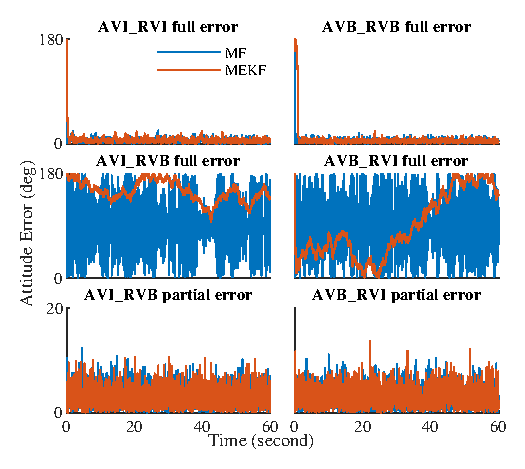
\includegraphics[scale=1.4]{figures/observability/attitudeError}
	\caption{Attitude errors for the matrix Fisher (MF) estimator and MEKF in four combinations of angular velocity and reference vector measurements. \label{fig:observability-attitudeError}}
\end{figure}

\begin{figure}
	\centering
	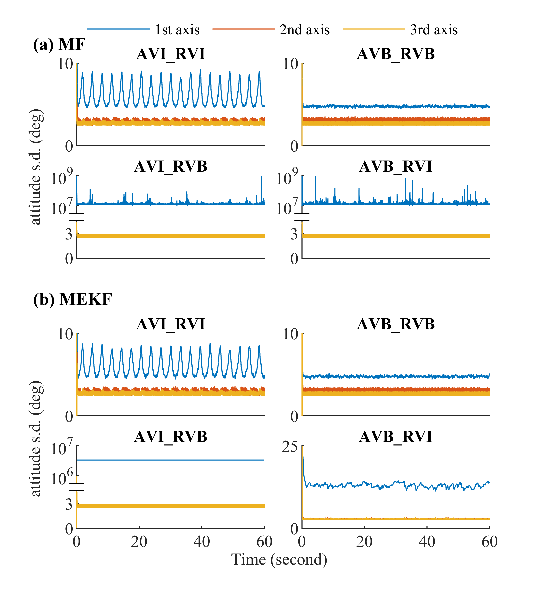
\includegraphics[scale=1.4]{figures/observability/attitudeStd}
	\caption[Attitude standard deviations for the matrix Fisher (MF) estimator and MEKF.]{Attitude standard deviations for the matrix Fisher (MF) estimator and MEKF.
		In the ``RVI'' and ``RVB'' cases, the attitude covariance matrix is expressed in the inertial and body-fixed frames respectively.
		For the MF filter, $(\tr{S}I_{3\times 3}-S)^{-1}$ is used as the attitude covariance matrix in the principal axes frame. \label{fig:observability-attitudeStd}}
\end{figure}

\begin{figure}
	\begin{subfigure}{0.45\textwidth}
		\centering
		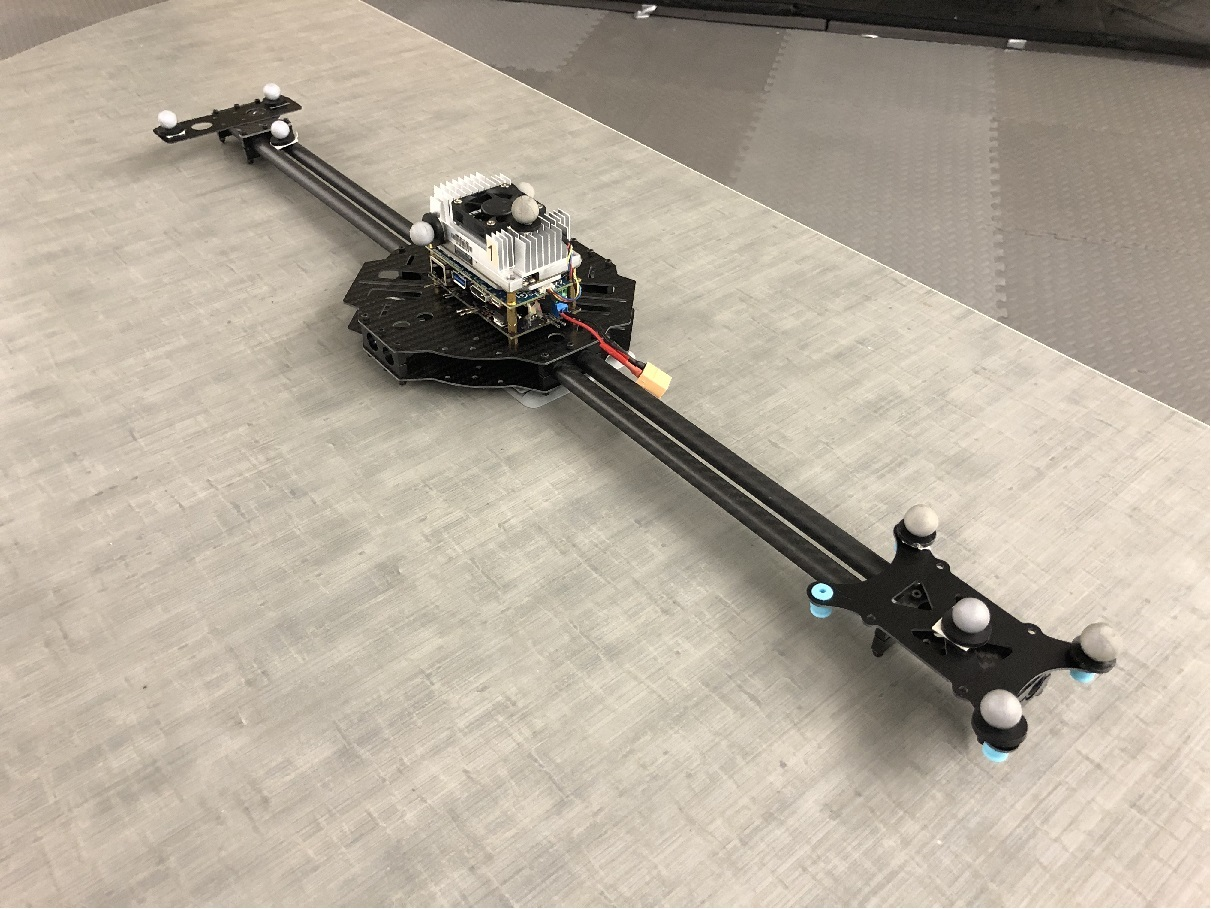
\includegraphics[width=\textwidth]{figures/observability/exp1.jpeg}
		\caption{Hardware configuration with reflective markers for a VICON motion capture system}
	\end{subfigure}
	\hspace{0.1\textwidth}
	\begin{subfigure}{0.45\textwidth}
		\centering
		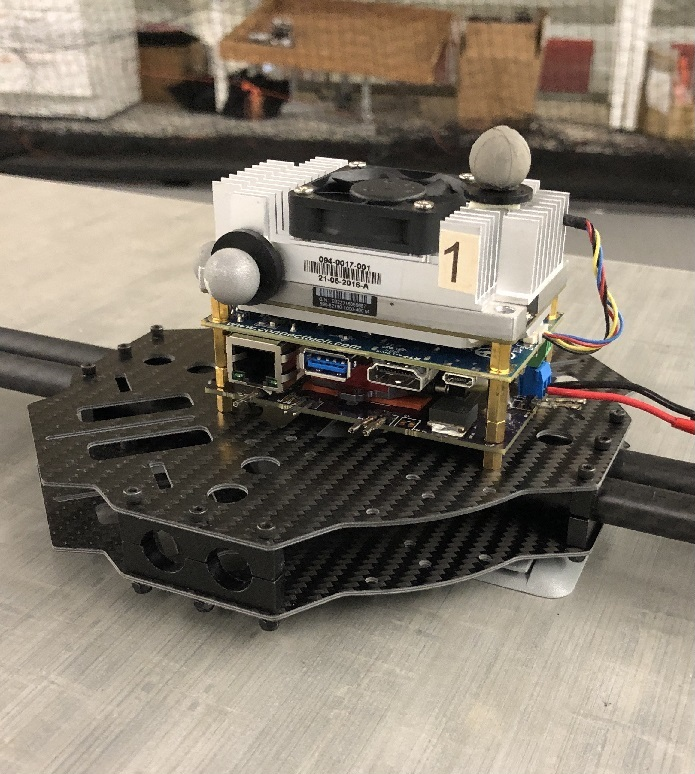
\includegraphics[width=\textwidth]{figures/observability/exp2.jpeg}
		\caption{Onboard computing module connected to IMU through a custom-made printed circuit board}
	\end{subfigure}
	\caption{Hardware platform for experiments.} \label{fig:observability-exp-hardware}
\end{figure}

The attitude observability was also validated through experiments.
We use a custom-made hardware platform (Figure \ref{fig:observability-exp-hardware}), which has been developed for autonomous unmanned aerial vehicles, to collect measurements while moving it with hands.
An external VICON motion capture system detects reflective markers attached to the platform to determine its attitude, which is used as the ground truth attitude.
A 9-axis inertial measurement unit (VectorNav VN100) is attached to the platform, and the onboard gyroscope provides the angular velocity measurement in the body-fixed frame, which is also converted into the angular velocity measurement in the inertial frame using the ground truth attitude. 
For the inertial direction measurement, the direction of gravity is measured by the accelerometer in IMU.
Moreover, for the body-fixed direction measurement, two additional markers are attached to the platform as a known and fixed reference vector in the body-fixed frame, which is measured by the Vicon motion system in the inertial frame.
All Vicon and IMU measurements are synchronized and sampled at \SI{100}{\hertz}, using an onboard Nvidia Jetson TX2 computing module.
The platform was rotated around its roll, pitch, and yaw axes during the data collection.
The matrix Fisher estimator and MEKF are run off-board using the collected experimental data, with the single vector measurement update applied at \SI{20}{\hertz}.
The noise parameters and initial conditions are set the same as in the simulation.
Note that these are not carefully tuned for the specific hardware, since the main objective is to verify the observability.

\begin{figure}
	\centering
	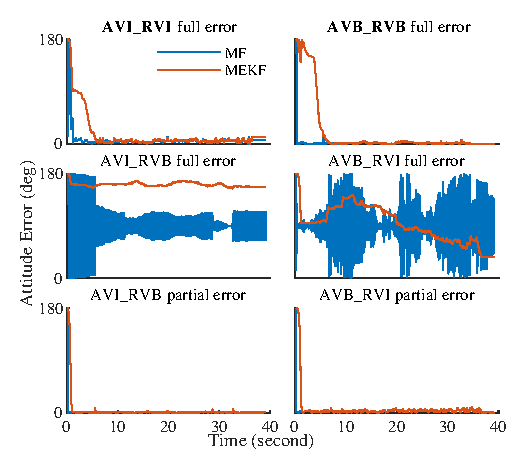
\includegraphics[scale=1.4]{figures/observability/attitudeError-Exp}
	\caption{Attitude errors for the matrix Fisher (MF) estimator and MEKF in four combinations of measurements with experimental data. \label{fig:observability-attitudeError-Exp}}
\end{figure}

\begin{figure}
	\centering
	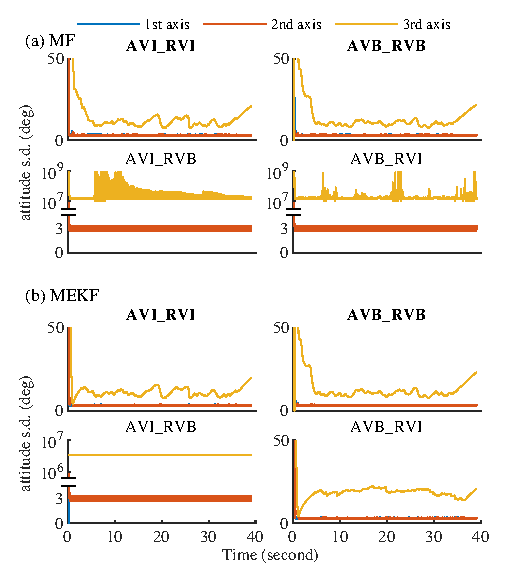
\includegraphics[scale=1.4]{figures/observability/attitudeStd-Exp}
	\caption[Attitude uncertainty for the matrix Fisher estimator (MF) and MEKF in four combinations of measurements with experimental data.]{Attitude uncertainty for the matrix Fisher estimator (MF) and MEKF in four combinations of measurements with experimental data.
		In the ``RVI'' cases, the attitude covariance matrix is expressed in the inertial frame; and in the ``RVB'' cases, it is expressed in the $b'$-$b''$-$b$ frame, where $b$ is the reference vector when resolved in the body-fixed frame, and $b',b''$ are perpendicular to $b$.
		For the MF filter, $(\tr{S}I_{3\times 3}-S)^{-1}$ is used as the attitude covariance matrix in the principal axes frame. \label{fig:observability-attitudeStd-Exp}}
\end{figure}

The attitude errors for the four combinations of measurements are presented in Figure \ref{table:observability-error} and Figure \ref{fig:observability-attitudeError-Exp}.
Similar with the simulation results, for the two observable cases (AVI\_RVI and AVB\_RVB) the full attitude error converges to around zero within \SI{10}{\second}; whereas for the two unobservable cases (AVI\_RVB and AVB\_RVI) only the partial error converges.
The standard deviation of the rotation vector is demonstrated in Figure \ref{fig:observability-attitudeStd-Exp}.
Again the uncertainties for the two observable cases are small in all three axes, but those for the two unobservable cases are only small in two axes, which is very similar to the simulation results.

\section{Attitude Estimation} \label{section:attEst}

In the previous section, a Bayesian attitude estimator is proposed to estimate the attitude with a gyroscope and repeated measurements of a single reference direction, in order to study attitude observability.
In \eqref{eqn:observability-kinematics-left}, it is assumed that the angular velocity measured from a gyroscope is affected by a white noise.
However, usually the gyroscope noise also contains a random walk term, referred to as the bias \cite{crassidis2007survey}.
As a random walk process, the gyroscope bias is time varying, and can easily deteriorate the integrated attitude in short time if it is not properly compensated for.
Therefore, an attitude estimator also needs to estimate the bias, simultaneously with the attitude.

Concurrent estimation of attitude and gyroscope bias has been studied in numerous works, as reviewed in Chapter \ref{section:intro-review-estimation}.
Nevertheless, most existing algorithms rely on variations of Kalman filter, which uses Gaussian distribution to model attitude dispersion, thus they cannot handle large attitude uncertainty as shown in Figure \ref{fig:wrapping}.
Although the matrix Fisher and Bingham distributions have been applied to deal with large uncertainty \cite{glover2014tracking,kurz2014recursive,lee2018bayesian}, they cannot estimate the gyroscope bias as the two distributions cannot model the correlation between attitude and gyroscope bias.

The introduction of matrix Fisher--Gaussian distribution in Chapter \ref{chap:MFG} was primarily motivated to use matrix Fisher distribution to deal with large attitude uncertainty, while estimating the gyroscope bias.
The correlation between attitude and bias is directly handled by the MFG in a global and singularity free fashion, allowing the attitude uncertainty to be very large.
In this section, a new recursive Bayesian attitude estimator is proposed based on MFG to estimate the attitude and gyroscope bias concurrently.

\subsection{Problem Formulation} \label{section:attEst-problem}

In this section, the following gyroscope kinematics is considered:
\begin{gather}
	R^T\diff{R} = (\hat{x}+\hat{\Omega})\diff{t} + (H_udW_u)^\wedge, \label{eqn:attEst-kinematics-att} \\
	\diff{x} = H_vdW_v \label{eqn:attEst-kinematics-bias},
\end{gather}
where $R\in\SO{3}$ is the attitude of a rigid body and $x\in\mathbb{R}^3$ is the bias of the onboard gyroscope.
The vector $\Omega\in\mathbb{R}^3$ is the angular velocity measured by the gyroscope that is resolved in the body-fixed frame.
Next, $W_u$ and $W_v\in\mathbb{R}^3$ are two independent three-dimensional Wiener processes, and $H_u, H_v \in \mathbb{R}^{3\times 3}$ are two matrices describing the strengths of noises.
The angular velocity measurement has two sources of noises: the bias term $x$ and the Gaussian white noise contributed by $H_u dW_u$.
The bias is slowly varying while being driven by another white noise $H_v dW_v$.

The stochastic differential equation \eqref{eqn:attEst-kinematics-att} is interpreted in the Stratonovich sense to guarantee the process does not leave $\SO{3}$ \cite{barrau2018stochastic,markley2006attitude}.
Let the time be discretized by a sequence $\{t_0,t_1,\ldots\}$. 
For convenience, it is assumed that the time step $h\in\mathbb{R}$ is fixed, i.e., $h= t_{k+1} - t_k$ for any $k$. 
According to \cite[Eqn. 14]{barrau2018stochastic}, the kinematics model can be discretized into
\begin{gather}
	R_{k+1} = R_k \exp\left\{ h (\hat{\Omega}_k+\hat{x}_k) + (H_u\Delta W_u)^\wedge \right\}, \label{eqn:attEst-kinematics-att-dist} \\
	x_{k+1} = x_k + H_v\Delta W_v,  \label{eqn:attEst-kinematics-bias-dist}
\end{gather}
where $\Delta W_u, \Delta W_v\in\mathbb{R}^{3\times 3}$ are the stochastic increments of the Wiener processes over the time step $h$, which are Gaussian with
\begin{equation}\label{eqn:attEst-kinematics-DeltaW}
	H_u\Delta W_u \sim \mathcal{N}(0,hG_u), \quad H_v\Delta W_v \sim \mathcal{N}(0,hG_v),
\end{equation}
where $G_u = H_uH_u^T$ and $G_v = H_vH_v^T\in\mathbb{R}^{3\times 3}$.

Two types of measurements are considered available at $t_k$, $k\geq 1$: (i) when the attitude is directly measured, and (ii) when reference directions in the inertial frame, such as the direction of magnetic field or gravity, are measured.
First, suppose the attitude is measured by $N_a$ attitude sensors as $Z_i\in\SO{3}$, whose error is distributed by the matrix Fisher distribution.
More specifically, given the true attitude $R_t\in\SO{3}$, the measurement error $R_t^TZ_i\in\SO{3}$ follows the matrix Fisher distribution with the parameter $F_{Z_i}\in\mathbb{R}^{3\times 3}$ for $i=1,\ldots, N_a$, which characterizes the accuracy and bias of the $i$-th attitude sensor. 

Next, suppose there are also $N_v$ fixed reference vectors ${a}_j\in\mathbb{S}^2$ in the inertial reference frame, which are measured by direction sensors in the body-fixed frame as ${z}_j\in\mathbb{S}^2$ for $j=1,\ldots,N_v$.
Furthermore, given the true attitude $R_t$, the noisy measurement ${z}_j$ is assumed to follow the von Mises--Fisher distribution \cite{mardia2009directional} with mean direction $R_t^TB_j{a}_j\in\mathbb{S}^2$ and concentration parameter $\kappa_j>0$.
The parameter $B_j\in\SO{3}$ specifies the constant bias of the direction sensor, and $\kappa_j$ specifies the concentration of its random noise.
The measurements $\Big\{\{Z_i\}_{i=1}^{N_a}, \{z_j\}_{j=1}^{N_v}\Big\}$ at time $t_k$ are altogether denoted by $\mathcal{Z}_k$.

The initial attitude and bias $(R_0,x_0)$ at $t_0$ are assumed to follow MFG with $n=3$ and $(\mu_0, \Sigma_0, P_0, U_0, S_0, V_0)$ of appropriate dimensions.
Given the gyroscope measurements $\{\Omega_k\}_{k=0}^\infty$, and the attitude and direction measurements $\{\mathcal{Z}_k\}_{k=1}^\infty$ at discrete time instants, the problem is to find the posterior distribution of $(R_k,x_k) | \{\mathcal{Z}_m\}_{m=1}^k$, and approximate it to an MFG with parameters $(\mu_k, \Sigma_k, P_k, U_k, S_k, V_k)$.
To find the posterior distribution, two steps are needed: first the uncertainty is propagated from $(R_k,x_k) | \{\mathcal{Z}_m\}_{m=1}^k$ to $(R_{k+1},x_{k+1}) | \{\mathcal{Z}_m\}_{m=1}^k$ according to the gyroscope kinematics equations \eqref{eqn:attEst-kinematics-att-dist} and \eqref{eqn:attEst-kinematics-bias-dist}.
Second, the prior distribution $(R_{k+1},x_{k+1}) | \{\mathcal{Z}_m\}_{m=1}^k$ is updated by the measurements $\mathcal{Z}_{k+1}$ using Bayes's formula into $(R_{k+1},x_{k+1}) | \{\mathcal{Z}_m\}_{m=1}^{k+1}$.
These two steps are developed using the MFG in the next two subsections.

\subsection{Uncertainty Propagation} \label{section:attEst-propagation}

Suppose $(R_k,x_k) | \{\mathcal{Z}_m\}_{m=1}^k \sim\mathcal{MG}(\mu_k, \Sigma_k, P_k, U_k, S_k, V_k)$. 
In this subsection, the expectations of $(R_{k+1},x_{k+1})$ used in the MLE of MFG are calculated to construct a new MFG describing the uncertainty of $(R_{k+1},x_{k+1})$.
The expectations are calculated in two different ways: (i) approximate analytical expressions are developed directly from the gyroscope kinematics, and (ii) they are approximated empirically using deterministically sampled sigma points.

Let us first look at how to develop analytical expressions for required moments.
The exponent in \eqref{eqn:attEst-kinematics-att-dist} can be decomposed into
\begin{align*}
	\{h(\Omega_k + \mu_k)\} + \{h(x_k-\mu_k) + H_u \Delta W_u\},
\end{align*}
after taking the hat map off. 
The first part is deterministic, and the second part is a random vector with zero mean.  
This leads to the following approximation to \eqref{eqn:attEst-kinematics-att-dist}.

\begin{lemma}
	Equation \eqref{eqn:attEst-kinematics-att-dist} is almost surely equivalent to
	\begin{align} \label{eqn:attEst-kinematics-att-factorization}
		R_{k+1} = & R_ke^{h(\hat{x}_k-\hat{\mu}_k) + (H_u\Delta W_u)^\wedge + o(h)} e^{h(\hat{\Omega}_k+\hat{\mu}_k)}.
	\end{align}
\end{lemma}
\begin{proof}
	Equation \eqref{eqn:attEst-kinematics-att-dist} is rewritten into 
	\begin{align*} 
		R_{k+1} &= R_k \left[ e^{h(\hat{\Omega}_k+\hat{x}_k) + (H_u\Delta W_u)^\wedge} 
		e^{-h(\hat{\Omega}_k+\hat{\mu}_k)} \right] e^{h(\hat{\Omega}_k+\hat{\mu}_k)}.
	\end{align*}
	The Baker-Campbell-Hausdorff (BCH) formula provides the solution of $Z$ to the equation $e^X e^Y = e^Z$ for given $X,Y$. 
	Applying this to the expression in the square brackets,  
	\begin{align} \label{eqn:attEst-kinematics-att-factorization-proof}
		R_{k+1} &= R_k e^{h(\hat{x}_k-\hat{\mu}_k) + (H_u\Delta W_u)^\wedge + A} e^{h(\hat{\Omega}_k+\hat{\mu}_k)},
	\end{align}
	where the additional term $A\in\so{3}$ is composed of at least twice iterated Lie brackets, and it is of the order of $h^2$ and $h\Delta W_u$.
	Since $\lim\limits_{h \to 0}\Delta W_u=0$ almost surely, $A \sim o(h)$.
\end{proof}

This lemma is helpful in making use of the closed form expression of the exponential map \eqref{eqn:rv2rot} for the deterministic components of \eqref{eqn:attEst-kinematics-att-dist}.
The uncertainty of $R_{k+1}$ contributed by the noises is quantified by the centered stochastic component $h(x_k-\mu_k) + H_u\Delta W_u$ with zero mean.
Next, an expression for $\expect{R_{k+1}}$ is derived to solve the marginal MLE.

\begin{theorem} \label{thm:attEst-prop-E(R_{k+1})}
	The expectation of the propagated attitude $R_{k+1}$ is given by
	\begin{align} \label{eqn:attEst-prop-E(R_{k+1})}
		\expect{R_{k+1}} = \left\{ \expect{R_k}\left( I_{3\times 3} + \tfrac{h}{2}(G_u-\tr{G_u}I_{3\times 3}) \right) + hU_k\expect{Q_kV_k^T\widehat{P_k\nu_{R_k}}} \right\} e^{h(\hat{\Omega}_k+\hat{\mu}_k)} + O(h^2),
	\end{align}
	where $Q_k=U_k^TR_kV_k$, $\nu_{R_k} = (Q_kS_k-S_kQ_k^T)^\vee$ for MFGI, or $\nu_{R_k} = (S_kQ_k-Q_k^TS_k)^\vee$ for MFGB.
\end{theorem}
\begin{proof}
	First, expand the first exponential term in \eqref{eqn:attEst-kinematics-att-factorization} into an infinite sum as
	\begin{align}
		e^{h (\hat x_k-\hat{\mu}_k) + (H_u\Delta W_u)^\wedge + o(h)} = \sum_{i=0}^\infty \tfrac{1}{i!}\left\{ h (\hat x_k-\hat{\mu}_k) + (H_u\Delta W_u)^\wedge + o(h) \right\}^i.
	\end{align}
	Note that (i) $\Delta W_u$ is a zero mean Gaussian vector with covariance matrix $hI_{3\times3}$, so its odd order moments are zero, and $\expect{\left((H_u\Delta W_u)^\wedge\right)^{2n}} \sim O(h^n)$; (ii) $o(h)$ in the above equation only has terms of order at least $h^2$ or $h\Delta W_u$ as shown in \eqref{eqn:attEst-kinematics-att-factorization-proof}.
	Combining these two observations, the first order approximation of $\expect{R_{k+1}}$ can be written as
	\begin{align} \label{eqn:attEst-prop-E(R_{k+1})-taylor}
		\expect{R_{k+1}} = \big\{ \expect{R_k} + h \expect{R_k(\hat x_k-\hat{\mu}_k)} + \tfrac{1}{2}\expect{R_k((H_u\Delta W_u)^\wedge)^2} \big\} e^{h(\hat{\Omega}_k+\hat{\mu}_k)} + O(h^2).
	\end{align}
	Then, since $(R_k,x_k)$ follows MFG,
	\begin{align*}
		\expect{R_k(\hat x_k-\hat{\mu}_k)} = \expect{R_k\widehat{P\nu_{R_k}}} = U_k\expect{Q_kV_k^T\widehat{P_k\nu_{R_k}}}.
	\end{align*}
	In addition, due to the independence of $R_k$ and $\Delta W_u$,
	\begin{align*}
		\expect{R_k((H_u\Delta W_u)^\wedge)^2} = h\expect{R_k}(G_u-\tr{G_u}I_{3\times 3}).
	\end{align*}
	Substituting the above two equations into \eqref{eqn:attEst-prop-E(R_{k+1})-taylor} yields \eqref{eqn:attEst-prop-E(R_{k+1})}.
\end{proof}

With the given $\expect{R_{k+1}}$, the marginal MLE for the attitude part of MFG can be solved as discussed in Chapter \ref{section:MFG-property}, which yields the estimates of $U_{k+1}$, $S_{k+1}$ and $V_{k+1}$.
Define $Q_{k+1} = U_{k+1}^TR_{k+1}V_{k+1}$, and $\nu_{R_{k+1}} = (Q_{k+1}S_{k+1}-S_{k+1}Q_{k+1}^T)^\vee$ for MFGI, or $\nu_{R_{k+1}} = (S_{k+1}Q_{k+1}-Q_{k+1}^TS_{k+1})^\vee$ for MFGB as the intermediate parameters for the MFG at time $t_{k+1}$.
Then the conditional MLE for the rest of parameters is solved as in Theorem \ref{thm:MFG-MLE-conditional} with the moments given as follows.

\begin{theorem} \label{thm:attEst-prop-otherMoments}
	Let $\tilde U, \tilde V\in\SO{3}$ and $\tilde S, \tilde{\tilde{V}}, \tilde{\tilde{S}} \in \mathbb{R}^{3\times 3}$ be
	\begin{gather*}
		\tilde{U} = U_{k+1}^T U_k, \quad 
		\tilde{V} = V_{k+1}^T e^{-h(\hat{\Omega}_k+\hat{\mu}_k)} V_k, \quad
		\tilde{S} = \tilde{U}^T S_{k+1} \tilde{V},\\
		\tilde{\tilde{V}} = V_{k+1}^T e^{-h(\hat{\Omega}_k+\hat{\mu})}G_u^TV_k, \quad
		\tilde{\tilde{S}} = \tilde{U}^TS_{k+1}\tilde{\tilde{V}}^T.
	\end{gather*}
	Also, let $\tilde{\nu}_R, \tilde{\tilde\nu}_R \in\mathbb{R}^3$, and $\Gamma_Q\in\mathbb{R}^{3\times 3}$ be
	\begin{subequations}
		\begin{flalign}
			\text{(MFGI)} && \tilde{\nu}_R &= (Q_k\tilde{S}^T-\tilde{S}Q_k^T)^\vee, && \\
			\text{(MFGB)} && \tilde{\nu}_R &= (\tilde{S}^TQ_k-Q_k^T\tilde{S})^\vee, && \\ \StepSubequations
			\text{(MFGI)} && \tilde{\tilde{\nu}}_R &= (Q_k\tilde{\tilde{S}}^T-\tilde{\tilde{S}}Q_k^T)^\vee, && \label{eqn:attEst-prop-vRTT-MFGI} \\
			\text{(MFGB)} && \tilde{\tilde{\nu}}_R &= (S_{k+1}\tilde{U}Q_k\tilde{\tilde{V}}^T - \tilde{\tilde{V}}Q_k^T\tilde{U}^TS_{k+1})^\vee. && \label{eqn:attEst-prop-vRTT-MFGB} \\ \StepSubequations
			\text{(MFGI)} && \Gamma_Q &= \left( \tr{Q_k\tilde{S}^T}I_{3\times 3} - Q_k\tilde{S}^T \right) Q_k && \label{eqn:attEst-prop-GammaQ-MFGI} \\
			\text{(MFGB)} && \Gamma_Q &= \tr{Q_k^T\tilde{S}}I_{3\times 3} - Q_k^T\tilde{S} && \label{eqn:attEst-prop-GammaQ-MFGB}
		\end{flalign}
	\end{subequations}
	Then, the moments $\expect{x_{k+1}}$, $\expect{\nu_{R_{k+1}}}$, and $\expect{x_{k+1}x_{k+1}^T}$ required for the conditional MLE are given by
	\begin{align}
		\expect{x_{k+1}} &= \mu_k, \label{eqn:attEst-prop-Ex_{k+1}} \\
		\expect{\nu_{R_{k+1}}} &= 0, \label{eqn:attEst-prop-EvR_{k+1}} \\
		\expect{x_{k+1}x_{k+1}^T} &= \expect{x_kx_k^T} + hG_v. \label{eqn:attEst-prop-Exx_{k+1}}
	\end{align}
	Also, the moments $\expect{x_{k+1}\nu_{R_{k+1}}^T}$ and $\expect{\nu_{R_{k+1}}\nu_{R_{k+1}}^T}$ are
	\begin{subequations} \label{eqn:attEst-prop-ExvR_{k+1}}
		\allowdisplaybreaks
		\begin{flalign}
			\text{(MFGI)} && &\expect{x_{k+1}\nu_{R_{k+1}}^T} = \Big[ P_k\Big( \expect{\nu_{R_k}\tilde{\nu}_R^T} + \tfrac{h}{2}\expect{\nu_{R_k}\tilde{\tilde{\nu}}_R^T} - \tfrac{h\tr{G_u}}{2}\expect{\nu_{R_k}\tilde{\nu}_R^T} && \nonumber \\
			&& &\quad \quad + h\expect{\nu_{R_k}\nu_{R_k}^TP_k^TV_k\Gamma_Q^T} \Big) + \mu_k\Big( \expect{\tilde{\nu}_R^T} + \tfrac{h}{2}\expect{\tilde{\tilde{\nu}}_R^T} - \tfrac{h\tr{G_u}}{2}\expect{\tilde{\nu}_R^T} && \nonumber \\ 
			&& &\quad \quad + h\expect{\nu_{R_k}^TP_k^TV_k\Gamma_Q^T} \Big) + h\Sigma_{c_k}V_k\expect{\Gamma_Q^T} \Big]\tilde{U}^T + O(h^2), && \label{eqn:attEst-prop-ExvR_{k+1}-MFGI} \\
			\text{(MFGB)} && &\expect{x_{k+1}\nu_{R_{k+1}}^T} = \Big[ P_k\Big( \expect{\nu_{R_k}\tilde{\nu}_R^T} - \tfrac{h\tr{G_u}}{2}\expect{\nu_{R_k}\tilde{\nu}_R^T} 
			+ h\expect{\nu_{R_k}\nu_{R_k}^TP_k^TV_k\Gamma_Q^T} \Big) && \nonumber \\
			&& &\quad\quad + \mu_k\Big( \expect{\tilde{\nu}_R^T} - \tfrac{h\tr{G_u}}{2}\expect{\tilde{\nu}_R^T} + h\expect{\nu_{R_k}^TP_k^TV_k\Gamma_Q^T} \Big) + h\Sigma_{c_k}V_k\expect{\Gamma_Q^T} \Big] \tilde{V}^T && \nonumber \\
			&& &\quad\quad + \tfrac{h}{2}\Big( \mu_k\expect{\tilde{\tilde{\nu}}_R^T} + P_k\expect{\nu_{R_k}\tilde{\tilde{\nu}}_R^T} \Big) + O(h^2), && \label{eqn:attEst-prop-ExvR_{k+1}-MFGB}
		\end{flalign}
	\end{subequations}
	and
	\begin{subequations} \label{eqn:attEst-prop-EvRvR_{k+1}}
		\begin{flalign}
			\text{(MFGI)} && &\expect{\nu_{R_{k+1}}\nu_{R_{k+1}}^T} = \tilde{U} \Big[ \expect{\tilde{\nu}_R\tilde{\nu}_R^T} + h\expect{\Gamma_QV_k^TP_k\nu_{R_k}\tilde{\nu}_R^T} + h\expect{\tilde{\nu}_R\nu_{R_k}^TP_k^TV_k\Gamma_Q^T} && \nonumber \\
			&& &\qquad\qquad + h\expect{\Gamma_QV_k^TG_uV_k\Gamma_Q^T} -h\tr{G_u}\expect{\tilde{\nu}_R\tilde{\nu}_R^T} && \nonumber \\
			&& &\qquad\qquad + \tfrac{h}{2}\expect{\tilde{\nu}_R\tilde{\tilde{\nu}}_R^T} + \tfrac{h}{2}\expect{\tilde{\tilde{\nu}}_R\tilde{\nu}_R^T} \Big]\tilde{U}^T + O(h^2), && \label{eqn:attEst-prop-EvRvR_{k+1}-MFGI} \\
			\text{(MFGB)} && &\expect{\nu_{R_{k+1}}\nu_{R_{k+1}}^T} = \tilde{V} \Big( \expect{\tilde{\nu}_R\tilde{\nu}_R^T} + h\expect{\Gamma_QV_k^TP_k\nu_{R_k}\tilde{\nu}_R^T} 
			+ h\expect{\tilde{\nu}_R\nu_{R_k}^TP_k^TV_k\Gamma_Q^T} && \nonumber \\
			&& &\qquad\qquad + h\expect{\Gamma_QV_k^TG_uV_k\Gamma_Q^T} - h\tr{G_u}\expect{\tilde{\nu}_R\tilde{\nu}_R^T} \Big)\tilde{V}^T && \nonumber  \\
			&& &\qquad\qquad + \tfrac{h}{2}\big(\tilde{V}\expect{\tilde{\nu}_R\tilde{\tilde{\nu}}_R^T} 
			+ \expect{\tilde{\tilde{\nu}}_R\tilde{\nu}_R^T}\tilde{V}^T\big) + O(h^2). && \label{eqn:attEst-prop-EvRvR_{k+1}-MFGB}
		\end{flalign}
	\end{subequations}
\end{theorem}
\begin{proof}
	The proof of this theorem is a straightforward but tedious extension of Theorem \ref{thm:attEst-prop-E(R_{k+1})}.
	The detailed procedures are given in Appendix \ref{app:attEst-prop-otherMoments}.
\end{proof}

Note that $\nu_{R_k}$, $\tilde{\nu}_R$, $\tilde{\tilde{\nu}}_R$, and $\Gamma_Q$ are linear in $Q_k$ (see Lemma \ref{lemma:attEst-GammaQ}).
Therefore, the expectations on the right hand side of \eqref{eqn:attEst-prop-E(R_{k+1})}, \eqref{eqn:attEst-prop-ExvR_{k+1}} and \eqref{eqn:attEst-prop-EvRvR_{k+1}} can be calculated using the moments of $Q\sim \mathcal{M}(S_k)$ up to the third order.
More specifically, these expectations can be expressed as linear combinations of $\expect{Q_{ij}}$, $\expect{Q_{ij}Q_{kl}}$, $\expect{Q_{ij}Q_{kl}Q_{mn}}$ for $i,j,k,l,m,n \in \{1,2,3\}$, which can be evaluated using the formulae given in Appendix \ref{app:MF-moment-second-third}.
With these moments, the estimates for $(\mu_{k+1},\Sigma_{k+1},P_{k+1})$ can be constructed through the conditional MLE given in Theorem \ref{thm:MFG-MLE-conditional}. 
In summary, Theorem \ref{thm:attEst-prop-E(R_{k+1})} and Theorem \ref{thm:attEst-prop-otherMoments} provide an analytical approach to propagate $(R_k,x_k)\sim\mathcal{MG}(\mu_k,\allowbreak \Sigma_k,\allowbreak P_k,\allowbreak U_k,\allowbreak S_k,\allowbreak V_k)$ into $(R_{k+1},x_{k+1}) \sim \mathcal{MG}(\mu_{k+1},\allowbreak \Sigma_{k+1},\allowbreak P_{k+1},\allowbreak U_{k+1},\allowbreak S_{k+1},\allowbreak V_{k+1})$, up to accuracy $O(h^2)$ in moments.
The pseudocode for this analytical uncertainty propagation scheme is shown in Table \ref{tab:attEst-prop-analytical}.

\begin{table}
	\caption{Analytical uncertainty propagation for gyroscope kinematics}
	\label{tab:attEst-prop-analytical}
	\begin{algorithmic}[1]
		\algrule[0.8pt]
		\Procedure{$\mathcal{MG}(t_{k+1}) = $ Analytical Propagation}{$\mathcal{MG}(t_k),\Omega_k$}
		\algrule
		\State Calculate $\expect{R_{k+1}}$ using \eqref{eqn:attEst-prop-E(R_{k+1})}.
		\State Obtain $U_{k+1},S_{k+1},V_{k+1}$ according to the marginal MLE in Chapter \ref{section:MFG-property} using $\expect{R_{k+1}}$.
		\State Calculate the moments in Theorem \ref{thm:attEst-prop-otherMoments}.
		\State Obtain $\mu_{k+1},\Sigma_{k+1},P_{k+1}$ according to Theorem \ref{thm:MFG-MLE-conditional} using the moments calculated in Step 4.
		\State Set $\mathcal{MG}(t_{k+1}) = \mathcal{MG}(\mu_{k+1},\Sigma_{k+1},P_{k+1},U_{k+1},S_{k+1},V_{k+1})$.
		\EndProcedure
		\algrule[0.8pt]
	\end{algorithmic}
\end{table}

Next, an alternative sampling-based method is presented to propagate the uncertainty using unscented transform.
In contrast to the preceding analytical approach, the unscented transform selects so called sigma points from the distribution of $(R_k,x_k)$, which are propagated through \eqref{eqn:attEst-kinematics-att-dist} and \eqref{eqn:attEst-kinematics-bias-dist}, and then they are matched to a new MFG using MLE.
The sigma points are selected in a deterministic fashion to characterize the mean and dispersion of the distribution.
To do this, first a canonical form of MFG is given where the mean values are centered, and all the correlations are eliminated.
\begin{lemma}
	Let $(R,x)\sim \mathcal{MG}(\mu,\Sigma,P,U,S,V)$.
	Define $Q = U^TRV\in\SO{3}$, and $y = \Sigma_c^{-1/2}(x-\mu-P\nu_R)\in\mathbb{R}^n$, then $(Q,y)$ follows $\mathcal{MG}(0,I,0,I,S,I)$.
\end{lemma}
\begin{proof}
	After change of variables, it can be easily seen that $\diff y \diff Q = \det(\Sigma_c^{-1/2}) \diff x \diff R$.
	Then the probability measure of $(Q,y)$ becomes
	\begin{align*}
		p(R,x) \diff x \diff R =  \frac{1}{c(S)\sqrt{(2\pi)^n}} \expb{-\tfrac{1}{2}y^Ty} \etr{SQ^T} \diff y \diff Q
	\end{align*}
	according to \eqref{eqn:MFG-density}, which finishes the proof.
\end{proof}

In the above canonical form, the Gaussian part is decoupled from the matrix Fisher part. 
As such, the sigma points of the canonical MFG are the union of the sigma points for the Gaussian distribution and those for the matrix Fisher distribution \cite{lee2018bayesian}.
These can be transformed back to the original MFG according to the above theorem as follows.

\begin{definition} \label{def:MFG-sigmaPoints}
	Consider $\mathcal{MG}(\mu,\Sigma,P,U,S,V)$.
	Define the $7+2n$ sigma points for its canonical distribution as
	\begin{gather} \label{eqn:attEst-unscented-sigmaPoints}
		({Q},y)_{1,2} = \left(\exp(\pm\theta_1\hat{e}_1),[0,\ldots,0]^T\right), \nonumber \\
		({Q},y)_{3,4} = \left(\exp(\pm\theta_2\hat{e}_2),[0,\ldots,0]^T\right), \nonumber \\
		({Q},y)_{5,6} = \left(\exp(\pm\theta_3\hat{e}_3),[0,\ldots,0]^T\right), \nonumber \\
		({Q},y)_{7,8} = \left(I_{3\times3},\left[\pm\sqrt{\frac{n}{w_G}},0,\ldots,0\right]^T\right), \nonumber \\
		\vdots \nonumber \\
		({Q},y)_{5+2n,6+2n} = \left(I_{3\times3},\left[0,\ldots,0,\pm\sqrt{\frac{n}{w_G}}\right]^T\right), \nonumber \\
		({Q},y)_{7+2n} = \left(I_{3\times3},[0,\ldots,0]^T\right),
	\end{gather}
	where $0\leq \theta_i\leq \pi$ is chosen according to
	\begin{subnumcases}{\cos\theta_i= \label{eqn:attEst-unscented-theta}}
		\sigma + \dfrac{(1-\sigma)(\log c(S) - s_i)}{s_j+s_k},\; \mbox{ \text{if} $s_j+s_k\geq 1$},\\
		\left\{\sigma + (1-\sigma)(\log c(S) - s_i)+\tfrac{1}{2} \right\}(s_j+s_k)-\tfrac{1}{2},\; \mbox{ \text{else if} $0\leq s_j+s_k < 1$,}
	\end{subnumcases}
	for $i,j,k\in\mathcal{I}$.
	The weights for the first three pairs of sigma points are given by
	\begin{align}
		w_i = \frac{1}{4(1-\cos\theta_i)}\left\{\frac{1}{c(S)}\left(\frac{\partial c(S)}{\partial s_i}-\frac{\partial c(S)}{\partial s_j}-\frac{\partial c(S)}{\partial s_k}\right)+1\right\}
	\end{align}
	for $i=1,2,3$, where $\sigma$ in \eqref{eqn:attEst-unscented-theta} is chosen such that $2(w_1+w_2+w_3)=w_M$.
	The weights for the next $2n$ sigma points, namely from the $7$-th through $(6+2n)$-th sigma points are $\frac{w_G}{2n}$, and the weight for the last one is $w_0=1-w_M-w_G$.
	Let $R_i = U{Q}_iV^T$, and $x_i=\Sigma_c^{1/2}y_i+\mu+P\nu_{R_i}$.
	The sigma points for $\mathcal{MG}(\mu,\Sigma,P,U,S,V)$ are defined as $(R,x)_i$.
\end{definition}

In other words, each pair of sigma points are designed to capture the dispersion along each principal axis of MFG.
Parameters $w_M$, $w_G$ and $w_0$ are used to adjust the weights, respectively for the attitude, the linear components and the sigma point at identity.
This selection of sigma points is justified by the following theorem stating that the above sigma points recover the original MFG using the MLE of MFG.
\begin{theorem}
	The marginal-conditional MLE of the MFG is $(\mu,\Sigma,P,U,S,V)$ with the sigma points given in Definition \ref{def:MFG-sigmaPoints}.
\end{theorem}
\begin{proof}
	The marginal MLE is the same as the MLE of matrix Fisher distribution, and it has been proved in \cite[Theorem IV.1]{lee2018bayesian} that the sigma points recovers $U$, $S$, and $V$.
	For the conditional MLE, it is easy to see that $\expectbar{y}=0$, $\expectbar{\nu_R}=0$, and $\expectbar{y\nu_R^T}=0$.
	Then, it can be shown that
	\begin{align*}
		&\covbar{x}{\nu_R} = P\covbar{\nu_R}{\nu_R} \\
		&\expectbar{x} = \mu \\
		&\covbar{x}{x} = \Sigma_c + P\covbar{\nu_R}{\nu_R}P^T.
	\end{align*}
	According to Theorem \ref{thm:MFG-MLE-conditional}, these prove the conditional MLE with the sigma points recovers the parameters $P$, $\mu$, and $\Sigma$.
\end{proof}

It should be noted that another unscented transform for the Bingham distribution has been proposed in \cite{gilitschenski2015unscented}, which can also be applied to the matrix Fisher distribution using the Lie group homomorphism \eqref{eqn:SO3-Sph3}.
Its difference with the first six sigma points in \eqref{eqn:attEst-unscented-sigmaPoints} is that it does not require the six sigma points have equal density.
A benefit of the unscented transform in \cite{gilitschenski2015unscented} is that it only uses the first order moment $D$, so there is no need to solve \eqref{eqn:MF-S2D} if $S$ is unknown.

Given $(R_k,x_k)\sim\mathcal{MG}(\mu_k,\Sigma_k,P_k,U_k,S_k,V_k)$, $7+2n= 13$ sigma points are selected from the MFG as in Definition \ref{def:MFG-sigmaPoints}, together with 7 sigma points from the noise $H_u\Delta W_u$ in \eqref{eqn:attEst-kinematics-DeltaW} according to the common unscented transform for a Gaussian distribution in $\mathbb{R}^3$ (for example, see \cite[Chapter 9]{haug2012bayesian}).
These sigma points are propagated to $t_{k+1}$ through the discrete kinematics model \eqref{eqn:attEst-kinematics-att-dist} and \eqref{eqn:attEst-kinematics-bias-dist} without the noise term $H_v\Delta W_v$.
Then a new MFG at $t_{k+1}$ is recovered from these propagated sigma points using the MLE introduced in Chapter \ref{section:MFG-property}.
The effect of the noise term $H_v\Delta W_v$ driving the gyro bias in \eqref{eqn:attEst-kinematics-bias-dist} is accounted by adding $hG_v$ to the new covariance matrix $\Sigma_{k+1}$ for $x_{k+1}$, according to the following Proposition \ref{thm:MFG-addGauss}.
The pseudocode for this uncertainty propagation scheme is summarized in Table \ref{tab:attEst-prop-unscented}.

\begin{theorem} \label{thm:MFG-addGauss}
	Suppose $(R,x)\sim\mathcal{MG}(\mu,\allowbreak \Sigma,\allowbreak P,\allowbreak U,\allowbreak S,\allowbreak V)$ and $x'\sim\mathcal{N}(\mu',\Sigma')$, and they are mutually independent.
	Then $(R,x+x') \sim \mathcal{MG}(\mu+\mu',\allowbreak \Sigma+\Sigma',\allowbreak P,\allowbreak U,\allowbreak S,\allowbreak V)$.
\end{theorem}
\begin{proof}
	Let $y=x+x'$, then the density function for $(R,y)$ is
	\begin{align*}
		f_{R,y}(R,y) &= \int_{x\in\mathbb{R}^n} f_{R,x}(R,x)f_{x'}(y-x) \diff x \\
		&= \frac{1}{c}\int_{x\in\mathbb{R}^n} \etr{FR^T} \expb{-\tfrac{1}{2}(x-\mu_c)^T\Sigma_c^{-1}(x-\mu_c)} \\ 
		&\qquad\qquad \cdot \expb{-\tfrac{1}{2}(y-x-\mu')^T(\Sigma')^{-1}(y-x-\mu')} \diff x \\
		&= \frac{1}{c'} \etr{FR^T} \expb{-\tfrac{1}{2}(y-\mu_c-\mu')^T (\Sigma_c+\Sigma')^{-1} (y-\mu_c-\mu') },
	\end{align*}
	where $c$, $c'$ are some normalizing constants, and the last equality is from the addition of two independent Gaussian random vectors.
	Comparing the above equation with \eqref{eqn:MFG-density} yields the desired result.
\end{proof}

\begin{table}
	\caption{Unscented uncertainty propagation for gyroscope kinematics \label{tab:attEst-prop-unscented}}
	\begin{algorithmic}[1]
		\algrule[0.8pt]
		\Procedure{$\mathcal{MG}(t_{k+1}) = $ Unscented Propagation}{$\mathcal{MG}(t_k),\Omega_k$}
		\algrule
		\State Select sigma points and weights $\{(R,x,w)_i\}_{i=1}^{13}$ from $\mathcal{MG}(t_k)$.
		\State Select sigma points and weights $\{(H_u\Delta W_u,w)_{j}\}_{j=1}^7$ from $\mathcal{N}({0},hG_u)$ according to the common unscented transform of a Gaussian distribution \cite{haug2012bayesian}.
		\State Propagate the sigma points through \eqref{eqn:attEst-kinematics-att-dist} and \eqref{eqn:attEst-kinematics-bias-dist} without the noise $H_v\Delta W_v$, i.e.,
		\begin{align*}
			R_{i,j} = R_i\exp(h(\hat{\Omega}_k + \hat{x}_i) + (H_u\Delta W_u)_j^\wedge), \qquad x_{i,j} = x_i,
		\end{align*}
		and calculate the weights as $w_{i,j}=w_iw_j$.
		\State Obtain $(\mu_{k+1},\Sigma_{k+1},P_{k+1},U_{k+1},S_{k+1},V_{k+1})$ from these $13 \times 7 = 91$ sigma points $(R,x,w)_{i,j}$ using the MLE of MFG in Chapter \ref{section:MFG-property}.
		\State Let $\Sigma_{k+1} = \Sigma_{k+1}+hG_v$
		\State Set $\mathcal{MG}(t_{k+1}) = \mathcal{MG}(\mu_{k+1},\Sigma_{k+1},P_{k+1},U_{k+1},S_{k+1},V_{k+1})$.
		\EndProcedure
		\algrule[0.8pt]
	\end{algorithmic}
\end{table}

\subsection{Measurement Update} \label{section:attEst-update}

After the uncertainty has been propagated from $(R_k,x_k) | \{\mathcal{Z}_m\}_{m=1}^k$ to $(R_{k+1},x_{k+1}) | \{\mathcal{Z}_m\}_{m=1}^k$ using the techniques introduced in the previous subsection, this subsection develops an algorithm to update the propagated MFG with the new measurement $\mathcal{Z}_{k+1}$ using Bayes' formula.
As the measurement update is assumed to be completed instantaneously at time $t_{k+1}$, the subscript $k+1$ is omitted throughout this subsection. 
The variables relevant to the posterior distribution conditioned by measurements are denoted by the superscript $+$.

Suppose the prior distribution of $(R,x)$ before measurement update follows MFG with parameters $(\mu,\Sigma,P,U,S,V)$. 
By the Bayes' rule and Theorem 3.2 in \cite{lee2018bayesian}, the posterior density conditioned on all of the available measurements $\mathcal{Z}$ is 
\begin{align} \label{eqn:attEst-update-density}
	p(R,x\lvert \mathcal{Z}) & \propto \etr{ \bigg( F + \sum_{i=1}^{N_a}Z_iF_i^T + \sum_{j=1}^{N_v}\kappa_jB_ja_jz_j^T \bigg)R^T } \nonumber \\
	&\quad \cdot \expb{-\tfrac{1}{2}(x-\mu_c)^T\Sigma_c^{-1}(x-\mu_c)},
\end{align}
where $F$, $\mu_c$ and $\Sigma_c$ are defined as in Definition \ref{def:MFG} with respect to $(\mu,\Sigma,P,U,S,V)$.
The above posterior density of $(R,x)\lvert \mathcal{Z}$ is no longer MFG, as the tangent space at the mean attitude of the updated matrix Fisher part is altered.
Similar to the previous subsection, a new MFG with parameters $(\mu^+,\Sigma^+,P^+,U^+,S^+,V^+)$ is matched to this density through MLE after calculating the required moments.

\begin{theorem} \label{thm:attEst-update-moments}
	Define $F^+\in\mathbb{R}^{3\times 3}$ as
	\begin{align} \label{eqn:attEst-update-F}
		F^+ = F + \sum_{i=1}^{N_a}Z_iF_i^T + \sum_{j=1}^{N_v}\kappa_jB_ja_jz_j^T
	\end{align}
	and let its proper singular value decomposition be $F^+ = U^+ S^+ (V^+)^T$.
	Also, let
	\begin{subequations}
		\begin{flalign}
			\text{(MFGI)} && \nu^+_R &= (Q^+S^+-S^+(Q^+)^T)^\vee && \\
			\text{(MFGB)} && \nu^+_R &= (S^+Q^+-(Q^+)^TS^+)^\vee &&
		\end{flalign}
	\end{subequations}
	for $Q^+ = (U^+)^T R V^+\in\SO{3}$.
	Then the moments of the posterior density \eqref{eqn:attEst-update-density}, namely $\expect{ R\lvert \mathcal{Z} }$, $\expect{ \nu^+_R\lvert \mathcal{Z} }$ and $\expect{ \nu^+_R(\nu^+_R)^T\lvert \mathcal{Z} }$ are identical to their counterparts in Theorem \ref{thm:MFG-moment} after replacing $U,S,V$ with $U^+,S^+,V^+$, and
	\begin{align}
		\expect{ x \lvert \mathcal{Z} } & = {\mu}+P\expect{ \nu_R \lvert \mathcal{Z} }, \label{eqn:attEst-update-Ex} \\
		\expect{ xx^T \lvert \mathcal{Z} } & = {\mu}{\mu}^T+{\mu}\expect{ \nu_R \lvert \mathcal{Z} }^TP^T+P\expect{ \nu_R \lvert \mathcal{Z} }{\mu}^T 
		+P\expect{ \nu_R\nu_R^T \lvert \mathcal{Z} }P^T+{\Sigma}_c,\\
		\expect{ x(\nu^+_R)^T \lvert \mathcal{Z} } & = P\expect{ \nu_R(\nu^+_R)^T \lvert \mathcal{Z} } \label{eqn:attEst-update-Exv'R},
	\end{align}
	where
	\begin{subequations}
		\renewcommand{\theparentequation}{\arabic{parentequation}}
		\begin{flalign} \label{eqn:attEst-update-EvR}
			\text{(MFGI)} && \expect{\nu_R|\mathcal{Z}} &= \tilde{U}(\expect{Q^+|\mathcal{Z}}\tilde{S}^T - \tilde{S}\expect{Q^+|\mathcal{Z}}^T)^\vee, && \\
			\text{(MFGB)} && \expect{\nu_R|\mathcal{Z} } &= \tilde{V}(\tilde{S}^T\expect{Q^+|\mathcal{Z}} - \expect{Q^+|\mathcal{Z}}^T\tilde{S})^\vee, && \\ \StepSubequations
			\text{(MFGI)} && \expect{\nu_R\nu_R^T|\mathcal{Z}} &= \tilde{U} \expect{\tilde{\nu}_R^+(\tilde{\nu}_R^+)^T|\mathcal{Z}} \tilde{U}^T, && \\
			\text{(MFGB)} && \expect{\nu_R\nu_R^T|\mathcal{Z}} &= \tilde{V} \expect{\tilde{\nu}^+_R(\tilde{\nu}^+_R)^T|\mathcal{Z}} \tilde{V}^T, && \\  \StepSubequations
			\text{(MFGI)} && \expect{\nu_R(\nu_R^+)^T|\mathcal{Z}} &= \tilde{U} \expect{\tilde{\nu}_R^+(\nu_R^+)^T|\mathcal{Z}}, && \\
			\text{(MFGB)} && \expect{\nu_R(\nu_R^+)^T|\mathcal{Z}} &= \tilde{V} \expect{\tilde{\nu}_R^+(\nu_R^+)^T|\mathcal{Z}}, && \label{eqn:attEst-update-EvRv'R}
		\end{flalign}
	\end{subequations}
	with $\tilde U = U^TU^+$, $\tilde V = V^TV^+\in\SO{3}$, $\tilde{S} = \tilde U^T{S}\tilde V\in\mathbb{R}^{3\times 3}$, and $\tilde\nu^+_R\in\mathbb{R}^3$ is
	\begin{subequations}
		\begin{flalign}
			\text{(MFGI)} && \tilde{\nu}^+_R &= (Q^+\tilde{S}^T-\tilde{S}(Q^+)^T)^\vee, && \\
			\text{(MFGB)} && \tilde{\nu}^+_R &= (\tilde{S}^TQ^+-(Q^+)^T\tilde{S})^\vee. &&
		\end{flalign}
	\end{subequations}
\end{theorem}
\begin{proof}
	The expressions for $\expect{R \lvert \mathcal{Z}}$, $\expect{\nu^+_R \lvert \mathcal{Z}}$, $\expect{\nu^+_R(\nu^+_R)^T \lvert \mathcal{Z}}$, and \eqref{eqn:attEst-update-Ex}-\eqref{eqn:attEst-update-Exv'R} can be obtained by integrating these variables with respect to the density \eqref{eqn:attEst-update-density} similarly as in the proof of Theorem \ref{thm:MFG-moment}.
	Since $ Q = U^T R V = \tilde U Q^+ \tilde V^T$, for MFGB, it can be shown that
	\begin{equation*}
		\nu_R = (S\tilde UQ^+\tilde V^T-\tilde V(Q^+)^T \tilde U^TS)^\vee = \tilde{V}(\tilde{S}^TQ^+-(Q^+)^T\tilde{S})^\vee.
	\end{equation*}
	And for MFGI, the equation becomes
	\begin{equation*}
		\nu_R = (\tilde UQ^+\tilde V^TS-S\tilde V(Q^+)^T \tilde U^TS)^\vee = \tilde{U}(Q^+\tilde{S}^T-\tilde{S}(Q^+)^T)^\vee,
	\end{equation*}
	from which \eqref{eqn:attEst-update-EvR}-\eqref{eqn:attEst-update-EvRv'R} follow.
\end{proof}

Note that $\expect{\tilde{\nu}_R^+ (\tilde{\nu}_R^+)^T \lvert \mathcal{Z}}$ and $\expect{\tilde{\nu}_R^+ (\nu_R^+)^T \lvert \mathcal{Z}}$ can be expressed as linear combinations of $\expect{Q^+_{ij}Q^+_{kl} \lvert \mathcal{Z}}$ for $i,j,k,l\in\{1,2,3\}$, therefore they can be calculated using the second order moments of the matrix Fisher distribution $Q^+\lvert\mathcal{Z} \sim \mathcal{M}(S^+)$ given in Appendix \ref{app:MF-moment-second-third}.

Since the attitude part of \eqref{eqn:attEst-update-density} is already a matrix Fisher density, $U^+S^+(V^+)^T = F^+$ is the solution to the marginal MLE for the matrix Fisher part.
The conditional MLE is solved by Theorem \ref{thm:MFG-MLE-conditional} with the moments calculated above, which yields $\mu^+$, $\Sigma^+$ and $P^+$.
These provide the measurement update to represent the posterior distribution conditioned by the measurement as MFG.

The proposed uncertainty propagation and measurement update steps constitute a Bayesian attitude and gyro bias estimator. 
The current uncertainty represented by MFG can be propagated until an additional measurement is available, based on which the propagated uncertainty is updated. 
The estimates for the attitude and gyro bias are given by $UV^T$ and $\mu$, respectively. 
The pseudocode for the proposed Bayesian estimator is presented in Table \ref{tab:attEst-filter}.
A set of MATLAB codes for the proposed MFG and estimators are available at \cite{MFGCode}.

\begin{table}
	\caption{Bayesian estimation for attitude and gyroscope bias \label{tab:attEst-filter}}
	\begin{algorithmic}[1]
		\algrule[0.8pt]
		\Procedure{Estimation}{$\mathcal{MG}(t_0),\Omega(t),Z(t),z(t)$}
		\algrule
		\State Let $k=0$.
		\Repeat
		\State Either $\mathcal{MG}(t_{k+1})$ = Analytical Propagation($\mathcal{MG}(t_k)$,$\Omega(t_k)$) in Table \ref{tab:attEst-prop-analytical} or $\mathcal{MG}(t_{k+1})$ = Unscented Propagation($\mathcal{MG}(t_k)$,$\Omega(t_k)$) in Table \ref{tab:attEst-prop-unscented}.
		\State $k=k+1$.
		\Until $Z(t_{k+1})$ or $z(t_{k+1})$ ia available
		\State $\mathcal{MG}(t_{k+1})$ = Measurement Update($\mathcal{MG}(t_{k+1})$,$Z(t_{k+1})$,$z(t_{k+1})$).
		\State Obtain the estimates as $R(t_{k+1})=U_{k+1}V_{k+1}^T$, $x(t_{k+1})=\mu_{k+1}$ for $\mathcal{MG}(t_{k+1})$.
		\State \textbf{go to} step 3.
		\EndProcedure
		\algrule
		\Procedure{$\mathcal{MG}^+$ = Measurement Update}{$\mathcal{MG}^-$,$Z$,$z$}
		\State Compute $F^+$ from \eqref{eqn:attEst-update-F}, and calculate its proper SVD as $U^+S^+(V^+)^T=F^+$. 
		\State Calculate the moments of the posterior density in Theorem \ref{thm:attEst-update-moments}.
		\State Obtain $\mu^+,\Sigma^+,P^+$ according to Theorem \ref{thm:MFG-MLE-conditional}.
		\State Set $\mathcal{MG}^+ = \mathcal{MG}(\mu^+,\Sigma^+,P^+,U^+,S^+,V^+)$
		\EndProcedure
		\algrule[0.8pt]
	\end{algorithmic}
\end{table}

\subsection{Numerical Simulations}

In this section, the proposed Bayesian filter based on MFG is compared with the well-established MEKF through simulation studies.
Three simulation scenarios are tested (i) the attitude is directly measured;
(ii) two inertial reference directions are measured with various accuracy;
(iii) the magnetic direction is measured by a satellite orbiting the Earth.

\paragraph{Attitude Measurement}

In the first benchmark, a rotational motion of a rigid body is considered where the three Euler angles (body-fixed 3-2-1) follow sinusoidal waves with the frequency at \SI{0.35}{\hertz}, and the amplitudes of $\pi$, $\pi/2$ and $\pi$, respectively.
The corresponding average angular speed is \SI{6.17}{\radian/\second}.
The measured angular velocity is obtained from its true value by adding a bias and a white noise.
The gyroscope bias is modeled as a Wiener process (bias-instability noise) starting at zero with the isotropic strength $\sigma_v = $ \SI{500}{deg/\hour/\sqrt{\second}}, i.e., $H_v = \sigma_vI_{3\times3}$ in \eqref{eqn:attEst-kinematics-att}.
The white noise of angular velocity is Gaussian (angle random walk) with the isotropic strength $\sigma_u = $ \SI{10}{deg/\sqrt{\second}}, i.e., $H_u = \sigma_uI_{3\times3}$ in \eqref{eqn:attEst-kinematics-bias}.
These two values are greater than those of typical gyroscopes, but they are selected to generate large uncertainties favored by the MFG distribution.

The attitude measurement model for the proposed Bayesian estimator with MFG is given by
\begin{equation} \label{eqn:attEst-sim1-meaMFG}
	Z = R_t \delta R,
\end{equation}
where $R_t\in\SO{3}$ is the true attitude, and $\delta R\in\SO{3}$ follows a matrix Fisher distribution with the parameter $S_m = s_mI_{3\times 3}$.
This corresponds to the attitude measurement model introduced in Section \ref{section:attEst-update} without any constant bias.
The measurement equation for MEKF is not written as \eqref{eqn:attEst-sim1-meaMFG}. 
Instead, it is given by
\begin{equation} \label{eqn:attEst-sim1-meaMEKF}
	Z = R_t \exp(\delta\hat{\theta}),
\end{equation}
where $\delta\theta \in \mathbb{R}^3$ and $\delta\theta \sim \mathcal{N}(0,\sigma_mI_{3\times 3})$.
In order to fairly compare the proposed estimator based on MFG with MEKF, each estimator is simulated with both of \eqref{eqn:attEst-sim1-meaMFG} and \eqref{eqn:attEst-sim1-meaMEKF} after conversion. 
For example, when \eqref{eqn:attEst-sim1-meaMFG} is used in MEKF, $\log(\delta R)^\vee$, which corresponds to $\delta\theta$ in \eqref{eqn:attEst-sim1-meaMEKF}, is fitted into a Gaussian distribution.
Conversely, if \eqref{eqn:attEst-sim1-meaMEKF} is used in the MFG filter, $\exp(\delta\hat{\theta})$, which corresponds to  $\delta R$ in \eqref{eqn:attEst-sim1-meaMFG}, is fitted to a matrix Fisher distribution.

Three different levels of concentration are tested: (i) $s_m=2.4$, $\sigma_m=0.5$; (ii) $s_m=12$, $\sigma_m=0.2$; (iii) $s_m=200$, $\sigma_m=0.05$.
Therefore, case (i) has the greatest measurement noise among the three cases considered, and case (iii) has the lowest measurement noise. 
The initial distribution for attitude is the same as $Z$ in \eqref{eqn:attEst-sim1-meaMFG} (or \eqref{eqn:attEst-sim1-meaMEKF} for MEKF), the initial distribution for bias is $x_0\sim \mathcal{N}(0,0.1^2I_{3\times3})$, and they are independent.
The initial attitude and bias estimates are drawn randomly from these distributions.

The sampling frequencies for the gyroscope and the attitude measurements are \SI{150}{\hertz}, and \SI{30}{\hertz}, respectively.
Only the MFGI definition is used in the test, however, as the noise and initial conditions are isotropic, the filter based on MFGB is expected to behave very similarly to MFGI.
To test the estimators in a statistical sense, under each condition, sixty Monte Carlo simulations were conducted with the simulation time of 60 seconds.
The attitude and bias errors are averaged in each simulation, and further they are averaged over sixty simulations.
Paired $t$-tests ($N=60,\alpha=0.05$) were conducted between the two types of the proposed estimators based on MFG and MEKF.
Any significant statistical difference is indicated by $p<0.05$.

\begin{table*}
	\centering
	\caption{Attitude (\SI{}{deg}) and bias (\SI{}{deg/\second}) errors $\pm$ S.D. with attitude measurements \label{tab:attEst-sim1-error}}
	\footnotesize
	\begin{tabular}{l|c|ccc}
		Measurement &  & MFGI Analytical ($p$) & MFGI Unscented ($p$) & MEKF \\ \hline \hline
		\multirow{2}{*}{\eqref{eqn:attEst-sim1-meaMEKF} $\sigma_m$=0.5} & attitude & 11.94$\pm$0.40 ($<$0.001) & 11.94$\pm$0.40 ($<$0.001) & 11.88$\pm$0.41 \\
		& bias & 4.6$\pm$1.4 (0.81) & 4.6$\pm$1.4 (0.69) & 4.6$\pm$1.5 \\ \hline
		\multirow{2}{*}{\eqref{eqn:attEst-sim1-meaMFG} $s_m$=2.4} & attitude & 12.00$\pm$0.49 ($<$0.001) & 12.00$\pm$0.49 ($<$0.001) & 12.13$\pm$0.48 \\
		& bias & 5.0$\pm$1.7 (0.46) & 4.9$\pm$1.7 (0.42) & 5.0$\pm$1.8 \\ \hline \hline
		\multirow{2}{*}{\eqref{eqn:attEst-sim1-meaMEKF} $\sigma_m$=0.2} & attitude & 7.285$\pm$0.151 ($<$0.001) & 7.285$\pm$0.151 ($<$0.001) & 7.284$\pm$0.152 \\
		& bias & 3.79$\pm$1.11 (0.41) & 3.79$\pm$1.12 (0.47) & 3.79$\pm$1.13 \\ \hline
		\multirow{2}{*}{\eqref{eqn:attEst-sim1-meaMFG} $s_m$=12} & attitude & 7.449$\pm$0.182 (0.009) & 7.449$\pm$0.182 (0.015) & 7.450$\pm$0.181 \\
		& bias & 3.89$\pm$1.14 (0.09) & 3.89$\pm$1.14 (0.033) & 3.90$\pm$1.15 \\ \hline \hline
		\multirow{2}{*}{\eqref{eqn:attEst-sim1-meaMEKF} $\sigma_m$=0.05} & attitude & 3.54737$\pm$0.04250 (0.64) & 3.54741$\pm$0.04249 (0.009) & 3.54736$\pm$0.04251 \\
		& bias & 3.356$\pm$0.900 (0.97) & 3.357$\pm$0.903 (0.88) & 3.356$\pm$0.910 \\ \hline
		\multirow{2}{*}{\eqref{eqn:attEst-sim1-meaMFG} $s_m$=200} & attitude & 3.55406$\pm$0.04607 (0.21) & 3.55414$\pm$0.04606 (0.035) & 3.55409$\pm$0.04605 \\
		& bias & 3.722$\pm$0.939 (0.053) & 3.726$\pm$0.940 (0.031) & 3.733$\pm$0.940 \\ \hline \hline
	\end{tabular}
\end{table*}

The results for this simulation study are summarized in Table \ref{tab:attEst-sim1-error}.
It is shown that the accuracy for MFG based filters and MEKF are almost identical, with the differences in the attitude errors and the bias errors appearing mostly in the 3rd to 5th significant digits, if there is any.
The statistical differences found through $t$-tests are mainly caused by different measurement types, i.e., if $\delta R$ is used, MFG based filters are usually better than MEKF; conversely if $\delta\theta$ is used, MEKF is usually better.
This is natural since the measurement model for MFG based filters is formulated with $\delta R$, whereas that for MEKF is formulated with $\delta\theta$ \cite{lefferts1982kalman}, and there are some errors in matching a distribution of $\delta R$ to that of $\delta\theta$, and vice versa.
The only exception appears in $s_m=200$, where though $\delta R$ is used, the attitude error of MFG unscented filter is still greater than MEKF with the statistical significance of $p=0.035<0.05$.
Also, for $s_m=12$ and $s_m=200$, the bias error for MFG unscented filter is significantly smaller than MEKF.
But these differences are obviously negligible in practice.

\paragraph{Two Direction Measurements}

In this benchmark, the reference rotational motion of the rigid body and the gyroscope noise settings are chosen the same as the first test with attitude measurements.
Two reference directions in the inertial frame are assumed to be measured, given by
\begin{equation}
	z_{i} = R_t^T a_{i} + v_{i}
\end{equation}
for $i\in\{1,2\}$, and they are normalized to have unit lengths.
In the above equation, the reference directions are chosen as $a_1=e_2$ and $a_2=e_1$.
The true attitude is denoted by $R_t$, and $v_1,v_2$ are Gaussian noises distributed by $v_1 \sim \mathcal{N}(0,0.01I_{3\times3})$, $v_2 \sim \mathcal{N}(0,\sigma_2^2I_{3\times3})$. 
These follow the common MEKF and UKF frameworks in attitude estimation.
To simulate the proposed MFG filters, $a_i+v_i$ for $i=1,2$ are matched to von Mises--Fisher distributions by Monte Carlo sampling to obtain $\kappa_1,\kappa_2$ in \eqref{eqn:attEst-update-F} with $B_1 = B_2 = I_{3\times 3}$.
The gyroscope measurements are sampled at \SI{150}{\hertz}, and the two direction measurements are sampled at \SI{30}{\hertz}.
The simulation period is \SI{300}{\second}.

It is seen that in the first test with attitude measurements, the MFG filter and MEKF do not show too many differences in estimation accuracy.
This is because the attitude uncertainty is still not large enough to distinguish them.
In this benchmark, the two estimators are challenged with large uncertainty through two aspects.
First, the initial attitude $R_0$ is set as the true attitude rotated about its first body-fixed axis by \ang{180}, which is completely wrong.
The initial attitude uncertainty is set as $\delta R \sim \mathcal{N}(0,10^{10}I_{3\times3})$ for MEKF and UKF, which is very close to the uniform distribution, and it is matched to a matrix Fisher distribution through Monte Carlo sampling for MFG filters.
The initial bias is set as $x_0 = [0.2,0.2,0.2]^T$ \SI{}{\radian/\second} with the uncertainty $0.1^2 I_{3\times 3}$ given as the covariance, and the correlation between attitude and bias is zero.

\begin{table*}
	\centering
	\caption{Attitude (\SI{}{deg}) and bias (\SI{}{deg\per\second}) errors (S.D.) for different $\sigma_2$}
	\label{tab:attEst-sim2-error}
	\footnotesize
	\addtolength{\tabcolsep}{-1.5pt}
	\begin{tabular}{c|c|cccccc}
		\toprule
		$\sigma_2^2$ & & MEKF & UKF & MFGIA & MFGIU & MFGBA & MFGBU \\ \midrule
		\multirow{2}{*}{0.01} & full att. err. & 5.05(0.08) & 5.02(0.08) & 4.82(0.04)\textsuperscript{a,b} & 4.82(0.04)\textsuperscript{a,b} & 4.82(0.04)\textsuperscript{a,b} & 4.82(0.04)\textsuperscript{a,b} \\
		& bias error & 3.6(0.8) & 2.5(0.5) & 2.6(0.5)\textsuperscript{a} & 2.6(0.5)\textsuperscript{a} & 2.6(0.5)\textsuperscript{a} & 2.6(0.5)\textsuperscript{a} \\ \hline
		\multirow{2}{*}{0.1} & full att. err. & 7.06(0.25) & 6.95(0.16) & 6.67(0.11)\textsuperscript{a,b} & 6.67(0.11)\textsuperscript{a,b} & 6.67(0.11)\textsuperscript{a,b} & 6.67(0.11)\textsuperscript{a,b} \\
		& bias error & 4.0(0.9) & 2.6(0.5) & 2.8(0.5)\textsuperscript{a} & 2.8(0.5)\textsuperscript{a} & 2.8(0.5)\textsuperscript{a} & 2.8(0.5)\textsuperscript{a} \\ \hline
		\multirow{2}{*}{1} & full att. err. & 13.8(1.4) & 13.3(1.3) & 10.1(0.4)\textsuperscript{a,b} & 10.1(0.4)\textsuperscript{a,b} & 10.1(0.4)\textsuperscript{a,b} & 10.1(0.4)\textsuperscript{a,b} \\
		& bias error & 4.1(0.9) & 2.6(0.5) & 2.9(0.5)\textsuperscript{a,d} & 2.9(0.5)\textsuperscript{a,d} & 2.9(0.5)\textsuperscript{a,d} & 2.9(0.5)\textsuperscript{a,d} \\ \hline
		\multirow{2}{*}{5} & full att. err. & 51.0(17.4) & 44.4(11.7) & 14.4(0.9)\textsuperscript{a,b} & 14.4(0.9)\textsuperscript{a,b} & 14.4(0.9)\textsuperscript{a,b} & 14.4(0.9)\textsuperscript{a,b} \\
		& bias error & 5.6(2.3) & 3.1(0.8) & 3.0(0.5)\textsuperscript{a} & 3.0(0.5)\textsuperscript{a} & 2.9(0.5)\textsuperscript{a} & 2.9(0.5)\textsuperscript{a} \\ \hline
		\multirow{3}{*}{10} & full att. err. & 75.0(17.1) & 72.2(16.9) & 17.0(1.3)\textsuperscript{a,b} & 17.0(1.3)\textsuperscript{a,b} & 17.0(1.3)\textsuperscript{a,b} & 17.0(1.3)\textsuperscript{a,b} \\
		& par. att. err. & 4.19(0.12) & 4.11(0.05) & 4.00(0.04)\textsuperscript{a,b} & 4.00(0.04)\textsuperscript{a,b} & 4.00(0.04)\textsuperscript{a,b,e} & 4.00(0.04)\textsuperscript{a,b,e} \\
		& bias error & 6.7(4.1) & 3.4(0.9) & 3.0(0.5)\textsuperscript{a,b} & 3.0(0.5)\textsuperscript{a,b} & 3.0(0.5)\textsuperscript{a,b,e} & 3.0(0.5)\textsuperscript{a,b,e} \\ \hline
		\multirow{3}{*}{50} & full att. err. & 85.0(17.1) & 86.9(16.0) & 25.6(4.3)\textsuperscript{a,b} & 25.5(4.4)\textsuperscript{a,b} & 25.3(4.4)\textsuperscript{a,b,e} & 25.4(4.5)\textsuperscript{a,b} \\
		& par. att. err. & 4.19(0.06) & 4.11(0.05) & 4.01(0.04)\textsuperscript{a,b} & 4.01(0.04)\textsuperscript{a,b} & 4.00(0.04)\textsuperscript{a,b,e} & 4.00(0.04)\textsuperscript{a,b,e} \\
		& bias error & 6.5(2.7) & 3.5(1.0) & 3.3(0.6)\textsuperscript{a} & 3.3(0.6)\textsuperscript{a} & 3.1(0.6)\textsuperscript{a,b,e} & 3.1(0.6)\textsuperscript{a,b,e} \\ \hline
		\multirow{2}{*}{200} & par. att. err. & 4.19(0.06) & 4.11(0.05) & 4.02(0.04)\textsuperscript{a,b} & 4.01(0.04)\textsuperscript{a,b} & 4.00(0.04)\textsuperscript{a,b,e} & 4.00(0.04)\textsuperscript{a,b,e} \\
		& bias error & 6.5(2.6) & 3.5(1.0) & 5.0(1.0)\textsuperscript{a,d} & 4.3(1.0)\textsuperscript{a,d} & 3.4(0.7)\textsuperscript{a,e} & 3.4(0.8)\textsuperscript{a,e} \\ \hline
		\multirow{2}{*}{$\infty$} & par. att. err. & 4.24(0.11) & 4.10(0.06) & 4.20(0.05)\textsuperscript{a,d} & 4.16(0.05)\textsuperscript{a,d} & 3.99(0.04)\textsuperscript{a,b,e} & 3.99(0.04)\textsuperscript{a,b,e} \\
		& bias error & 6.5(2.4) & 3.7(1.1) & 20.1(1.4)\textsuperscript{c,d} & 18.7(1.6)\textsuperscript{c,d} & 3.6(0.8)\textsuperscript{a,e} & 3.7(0.8)\textsuperscript{a,e} \\ \bottomrule
	\end{tabular}
	
	\vspace{0.1cm}
	\raggedright
	\textsuperscript{a(c)} MFG filter is significantly better (worse) than MEKF; \\
	\textsuperscript{b(d)} MFG filter is significantly better (worse) than UKF; \\
	\textsuperscript{e} MFGB filter is significantly better than MFGI filter.
\end{table*}

Second, the accuracy $\sigma_2$ of the second direction measurement is varied as $\sigma_2^2 \in \{0.01,\allowbreak\ 0.1,\allowbreak\ 1,\allowbreak\ 5,\allowbreak\ 10,\allowbreak\ 50,\allowbreak\ 200,\allowbreak\ \infty\}$.
The first case of $\sigma_2^2=0.01$ corresponds to when the second vector measurement is as accurate as the first one.
As $\sigma_2$ is increased, the measurement becomes gradually less accurate, until it is no longer used when $\sigma_2^2 = \infty$.
The large uncertainty of $\sigma_2$ could lead to large uncertainty of the rotation around the first reference direction, and when $\sigma_2^2 = \infty$, this rotation becomes completely unobservable.

\begin{figure}
	\centering
	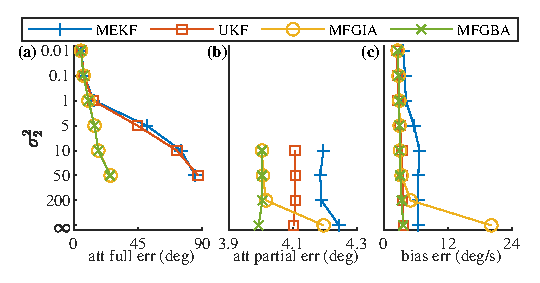
\includegraphics[scale=1.4]{figures/attEst-sim2-error}
	\caption[Estimation errors for varying accuracies of the second vector measurement.]{Estimation errors for varying accuracies of the second vector measurement: (a) full attitude error; (b) partial attitude error; (c) bias error for MEKF, UKF, MFGIA and MFGBA with varying $\sigma_2^2$.
		The errors of the unscented MFG filters are similar with the analytical MFG filters, and they are omitted for readability. \label{fig:attEst-sim2-error}}
\end{figure}

Six estimation schemes are compared, namely MEKF, UKF, two estimators with MFGB (one with the analytical propagation and the other with the unscented propagation, denoted respectively by MFGBA and MFGBU), and their counterparts with MFGI (denoted by MFGIA and MFGIU respectively).
For each case, one hundred Monte Carlo simulations (with respect to the random noise) are carried out.
Then, the attitude and bias errors are averaged across all time steps in one simulation, and further averaged across all simulations.
Paired $t$-tests ($N=100$, $\alpha=0.001$) are performed between MEKF, UKF and MFG filters, and between MFGB and MFGI to indicate any statistically significant difference.

The \textit{full} attitude error is defined as the angle between the true attitude and the estimated attitude.
As the second measurement becomes more inaccurate, the full attitude cannot be completely estimated because the rotation around the first reference vector becomes unobservable.
Thus, the \textit{partial} attitude error is defined as the angle between $R^T_t a_1$ and $R^Ta_1$, where $R_t$ and $R$ are the true attitude and the estimated attitude, respectively.
The partial attitude error only captures the accuracy along the first reference vector.
The simulation results are summarized in Table \ref{tab:attEst-sim2-error} and Fig. \ref{fig:attEst-sim2-error}.

When $\sigma_2^2 \in \{0.01,\ 0.1,\ 1\}$, the attitude error of the MFG filters is slightly lower than MEKF and UKF, and this advantage is mainly contributed by the faster initial convergence of MFG filters as illustrated in Fig. \ref{fig:attEst-sim2-trajectory-att}(a).
This is because for MEKF, the linearization of the measurement function is accurate only if the attitude error is small; and for UKF, the sigma points from a very large variance ($10^{10}$ in the initial step) suffer from the wrapping error, so they are unable to capture the large initial uncertainty.
The bias error of the MFG filters is also lower then MEKF, and is comparable to UKF (except when $\sigma_2^2=1$, UKF is statistically lower).

\begin{figure}
	\centering
	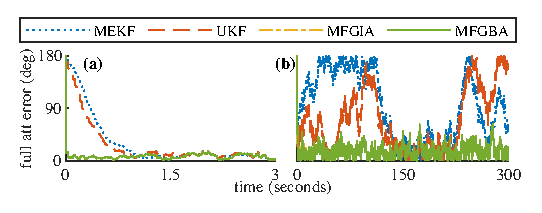
\includegraphics[scale=1.4]{figures/attEst-sim2-trajectory-att}
	\caption[Full attitude error for example simulations.]{(a) Full attitude error of MEKF, UKF, MFGIA and MFGBA for an example simulation ($\sigma_2^2 = 0.1$) during the first three seconds.
		(b) Full attitude error (\SI{0}{\second} to \SI{300}{\second}) for an example simulation ($\sigma_2^2 = 10$).
		The error of the unscented MFG filters is similar to the analytical MFG filters. \label{fig:attEst-sim2-trajectory-att}}.
\end{figure}

When $\sigma_2^2 \in \{5,\ 10,\ 50\}$, the full attitude error of the MFG filters is much lower than MEKF and UKF (Fig \ref{fig:attEst-sim2-trajectory-att}(b)).
This is because when the second vector measurement is inaccurate, the attitude uncertainty becomes highly dispersed along the rotation about the first reference vector, and the Gaussian distribution used by MEKF and UKF is incapable of modeling such large dispersion due to the wrapping error.
Also, the partial attitude error and bias error of the MFG filters are slightly lower than MEKF and UKF.
Next, comparing MFGB with MFGI, MFGB begins to exhibit some statistical advantages in partial attitude and bias errors, although their relative difference is still very small.
This difference can be attributed to that the attitude uncertainty becomes more non-isotropic as the second vector measurement becomes less accurate, so the distinction between the two definitions discussed in Chapter \ref{section:MFG-MFGI-MFGB} begins to emerge.
Because the gyroscope bias is resolved in the body-fixed frame, MFGB is more appropriate to model the correlation between attitude and bias than MFGI, this explains why the MFGB filter is more accurate.

When $\sigma_2^2 \in \{200,\ \infty\}$, MFGBA and MFGBU are still slightly more accurate than MEKF and UKF in partial attitude estimates, and more accurate than MEKF in bias estimation.
On the other hand, the performance of MFGIA and MFGIU in bias estimation degrades greatly, which affects the attitude error especially when $\sigma_2^2 = \infty$.
In Fig. \ref{fig:attEst-sim2-trajectory-bias}, the bias error of an example simulation ($\sigma_2^2=\infty$) is shown, where MFGIA and MFGIU make little corrections to the bias.
It turns out that there is little correlation built between the bias and attitude for MFGI during the uncertainty propagation, indicating that the attitude-bias correlation with non-isotropic attitude measurements cannot be modeled properly with MFGI.

\begin{figure}
	\centering
	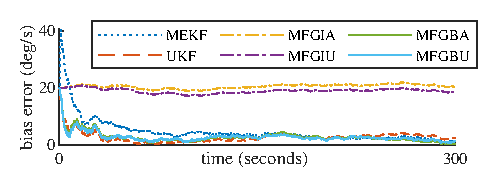
\includegraphics[scale=1.4]{figures/attEst-sim2-trajectory-bias}
	\caption{Bias error (\SI{0}{\second} to \SI{300}{\second}) in an example simulation ($\sigma_2^2=\infty$). \label{fig:attEst-sim2-trajectory-bias}}
\end{figure}

\paragraph{Magnetometer Measurement}

In this benchmark, a more realistic scenario is simulated where a satellite is orbiting around Earth with a single magnetometer and a gyroscope.
The orbital elements are given as follows, and three cases are considered for varying inclinations. 
\begin{equation*}
	a=6916\,\mathrm{km},\quad
	e=0.02,\quad
	\mathrm{\Omega} = 50^\circ,\quad
	\mathrm{\omega} = 0^\circ,\quad
	i = 0^\circ,\ 40^\circ \text{ or } 90^\circ.
\end{equation*}
According to the solution of the two-body problem, the orbital position with respect to the ECI frame, namely $r_{ECI}\in\mathbb{R}^3$, is computed at each time step.

A 3U CubeSat with the mass of $m=\SI{3}{\kilogram}$ is considered. The inertia matrix is given by
\begin{equation*}
	J=\diag[0.0325,\; 0.0325,\; 0.005]\,\SI{}{\kilogram\meter^2}.
\end{equation*}
The true attitude and the true angular velocity, namely $(R_{ref},\Omega_{ref})$ are generated according to the Euler's equation of motion
\begin{gather*}
	J\dot\Omega_{ref} + \Omega_{ref}\times J\Omega_{ref} =0,\\
	\dot R_{ref} = R_{ref}\hat\Omega_{ref},
\end{gather*}
where the initial condition is chosen as
\begin{gather*}
	R_{ref}(0)=I_{3\times 3},\quad \Omega_{ref}(0)=[0.05,\; 0.05,\; 0.02]\,\SI{}{\radian\per\second}.
\end{gather*}
These are numerically integrated with the geometric numerical integrator preserving the structures of $\SO{3}$, referred to as the Lie group variational integrator~\cite{lee2007lie,lee2007lie-b}, using the time step of $\SI{0.05}{\second}$. 

It is assumed that the angular velocity measurement is measured by a gyroscope at $\SI{20}{\hertz}$, i.e., $h=\SI{0.05}{\second}$.
The noise parameters for the gyroscope are: (i) angle random walk: $H_u=0.1I_{3\times 3}$, and (ii) bias instability: $H_v=0.0005I_{3\times 3}$, as indicated in \eqref{eqn:attEst-kinematics-att} and \eqref{eqn:attEst-kinematics-bias}.
The initial bias of the gyroscope is set as $[0.01,\; 0.01,\; 0.01]\, \SI{}{\radian\per\second}$.

\begin{figure}
	\centering
	\begin{subfigure}[b]{0.28\textwidth}
		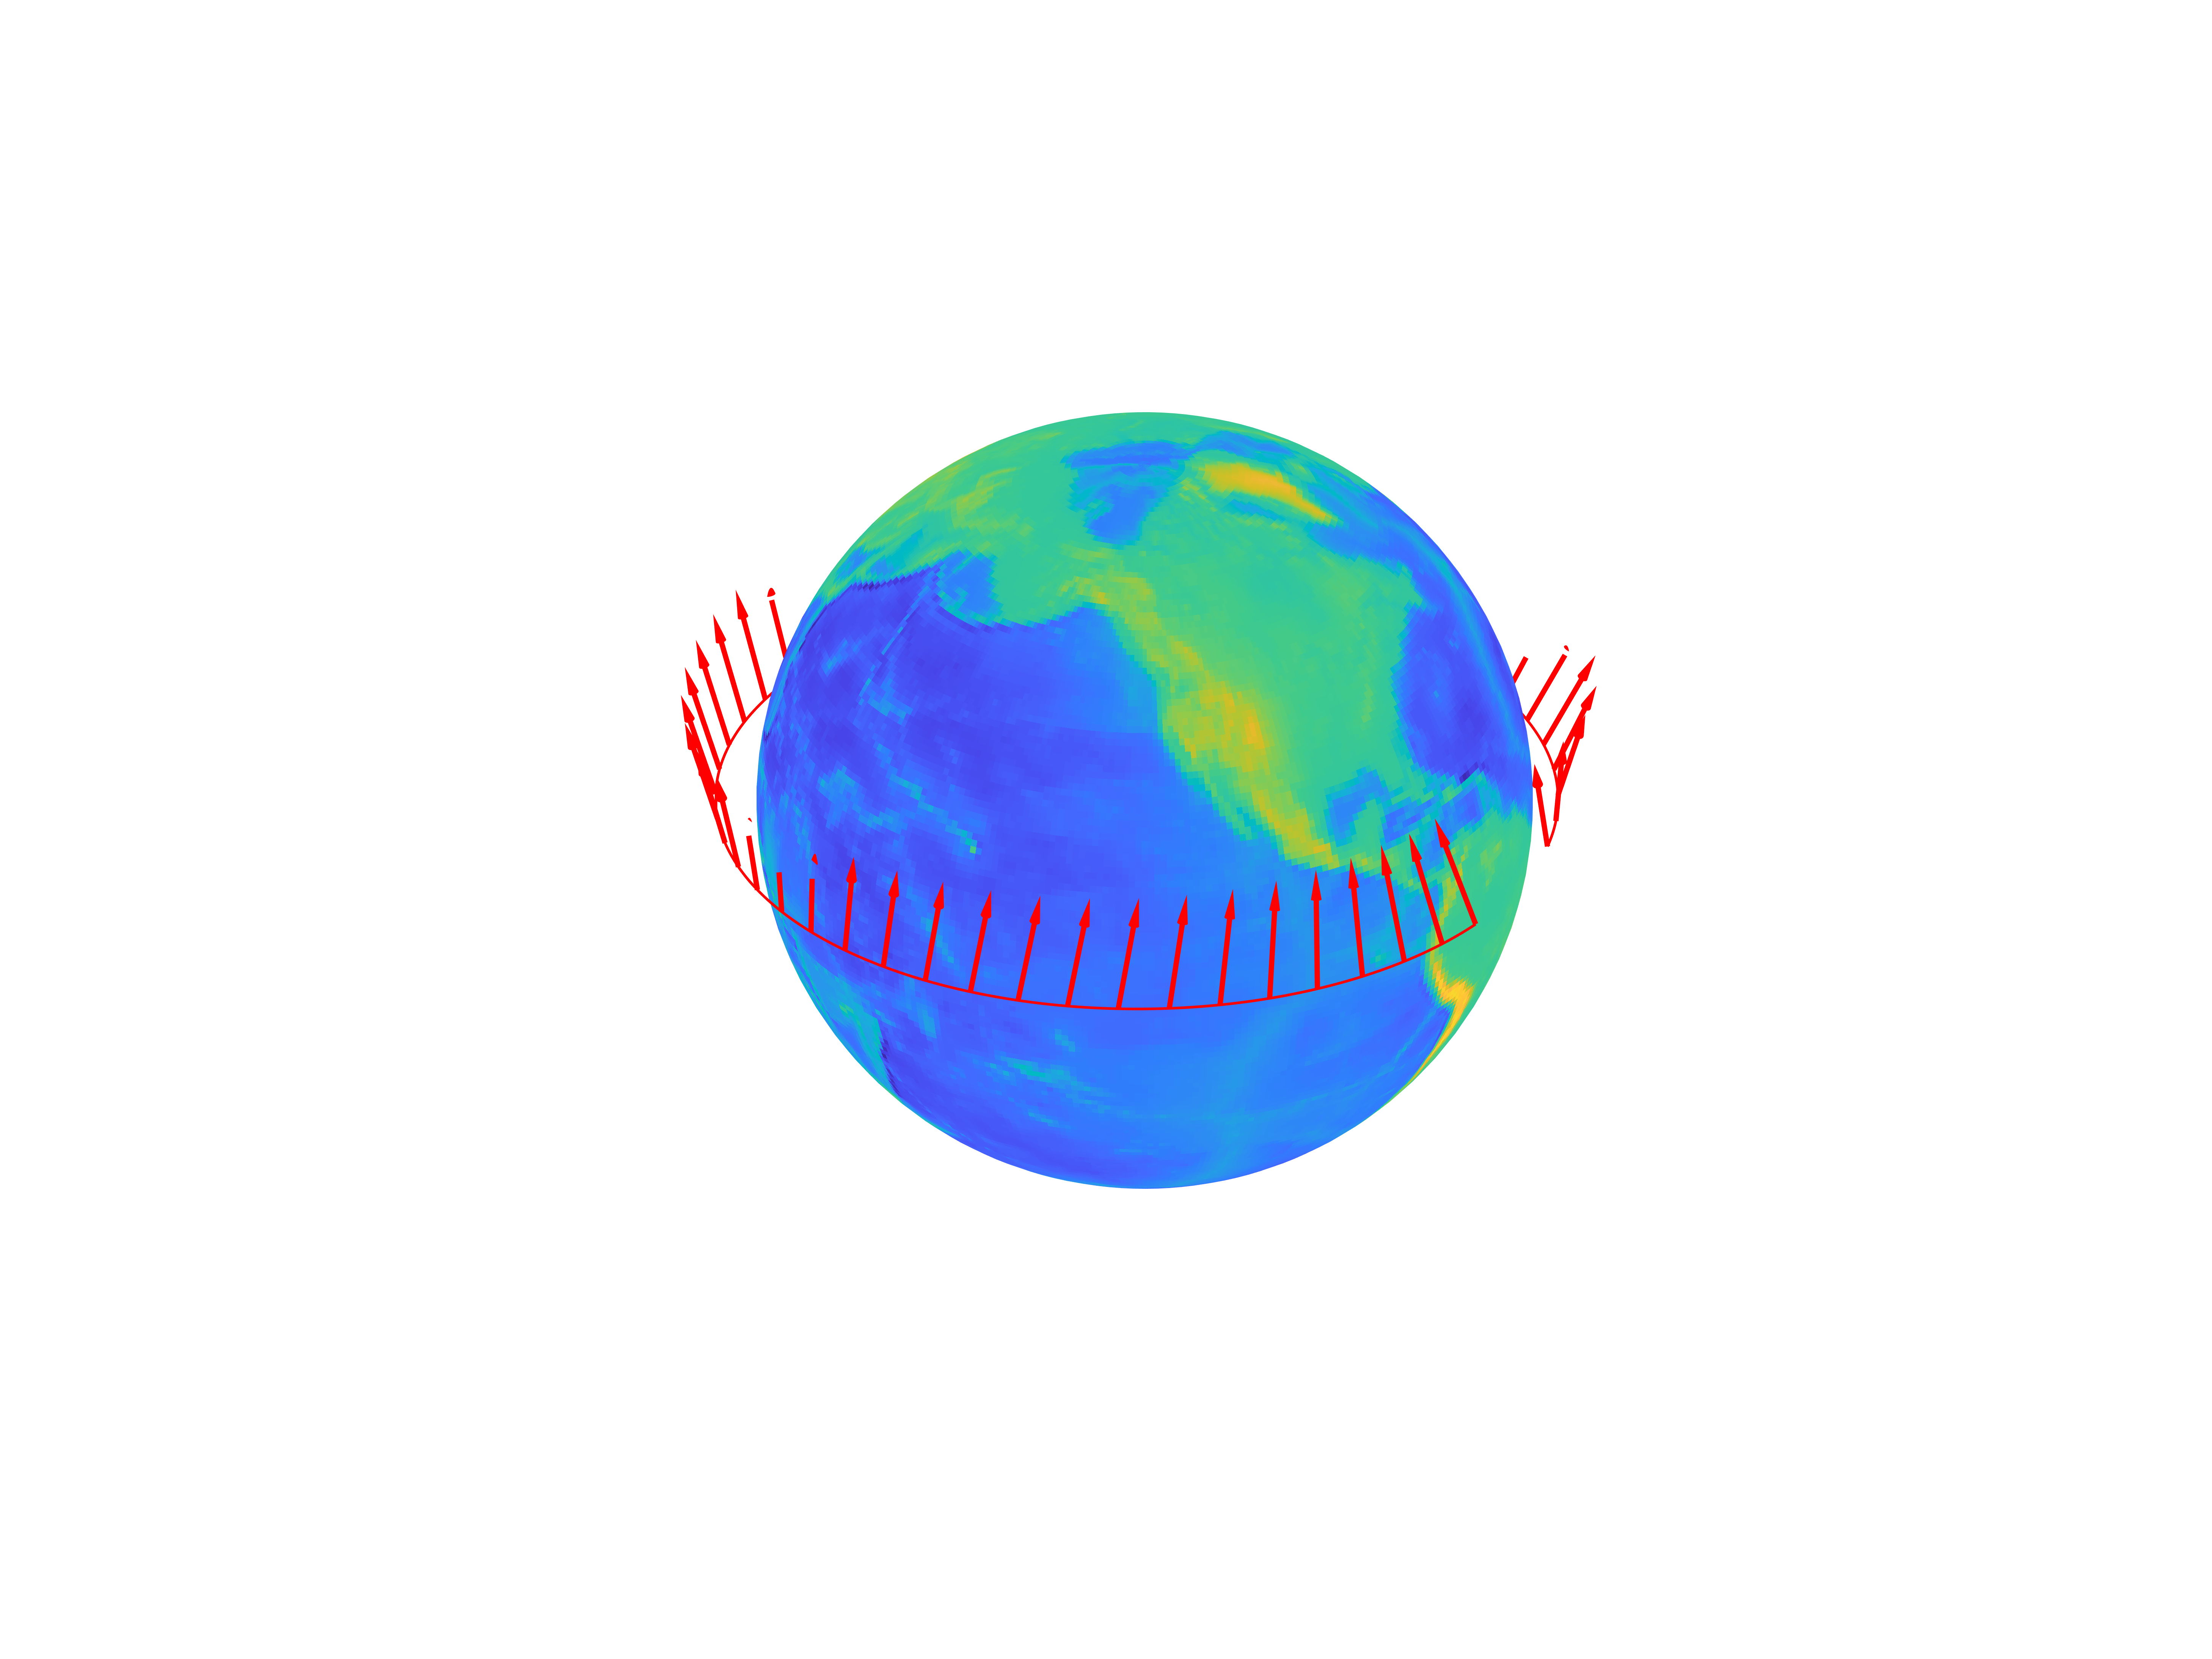
\includegraphics[trim={4.5cm 2.5cm 4cm 2.5cm},clip,width=1\textwidth]{figures/attEst-sim3-mag_0.png}
		\caption{$i=0^\circ$}
	\end{subfigure} \hspace{0.04\textwidth}
	\begin{subfigure}[b]{0.28\textwidth}
		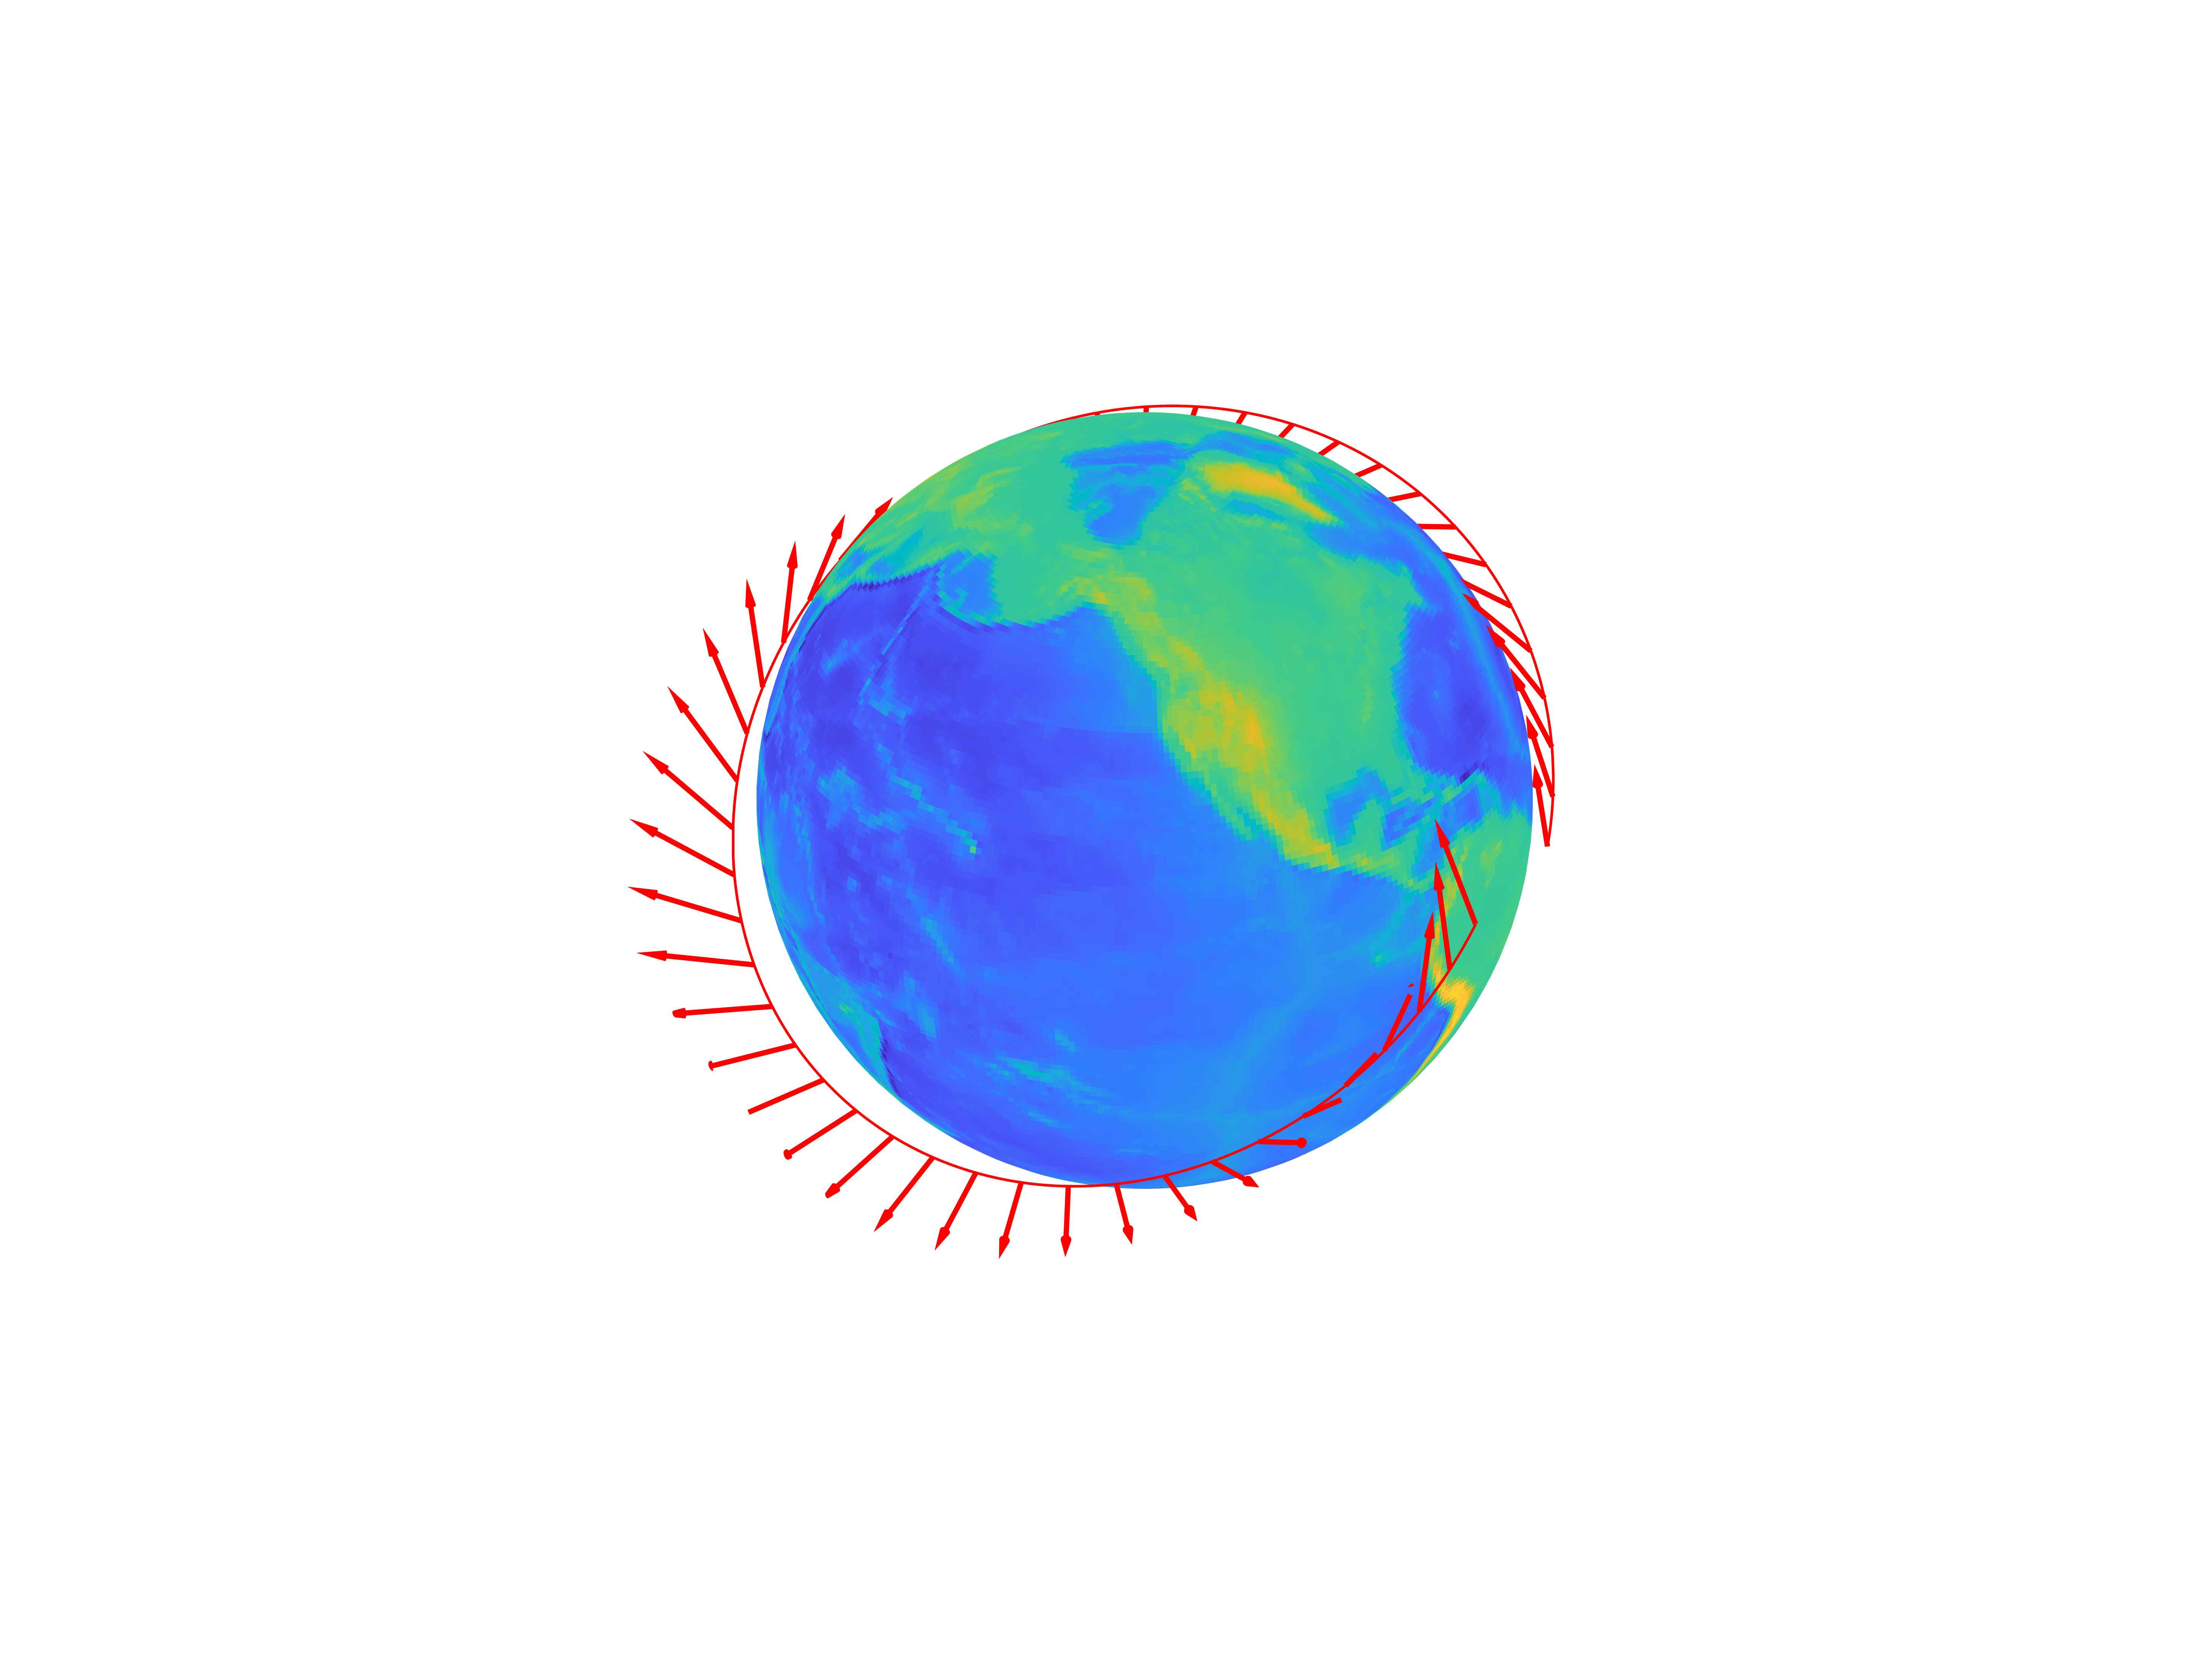
\includegraphics[trim={4.5cm 2.5cm 4cm 2.5cm},clip,width=1\textwidth]{figures/attEst-sim3-mag_40.png}
		\caption{$i=40^\circ$}
	\end{subfigure} \hspace{0.04\textwidth}
	\begin{subfigure}[b]{0.28\textwidth}
		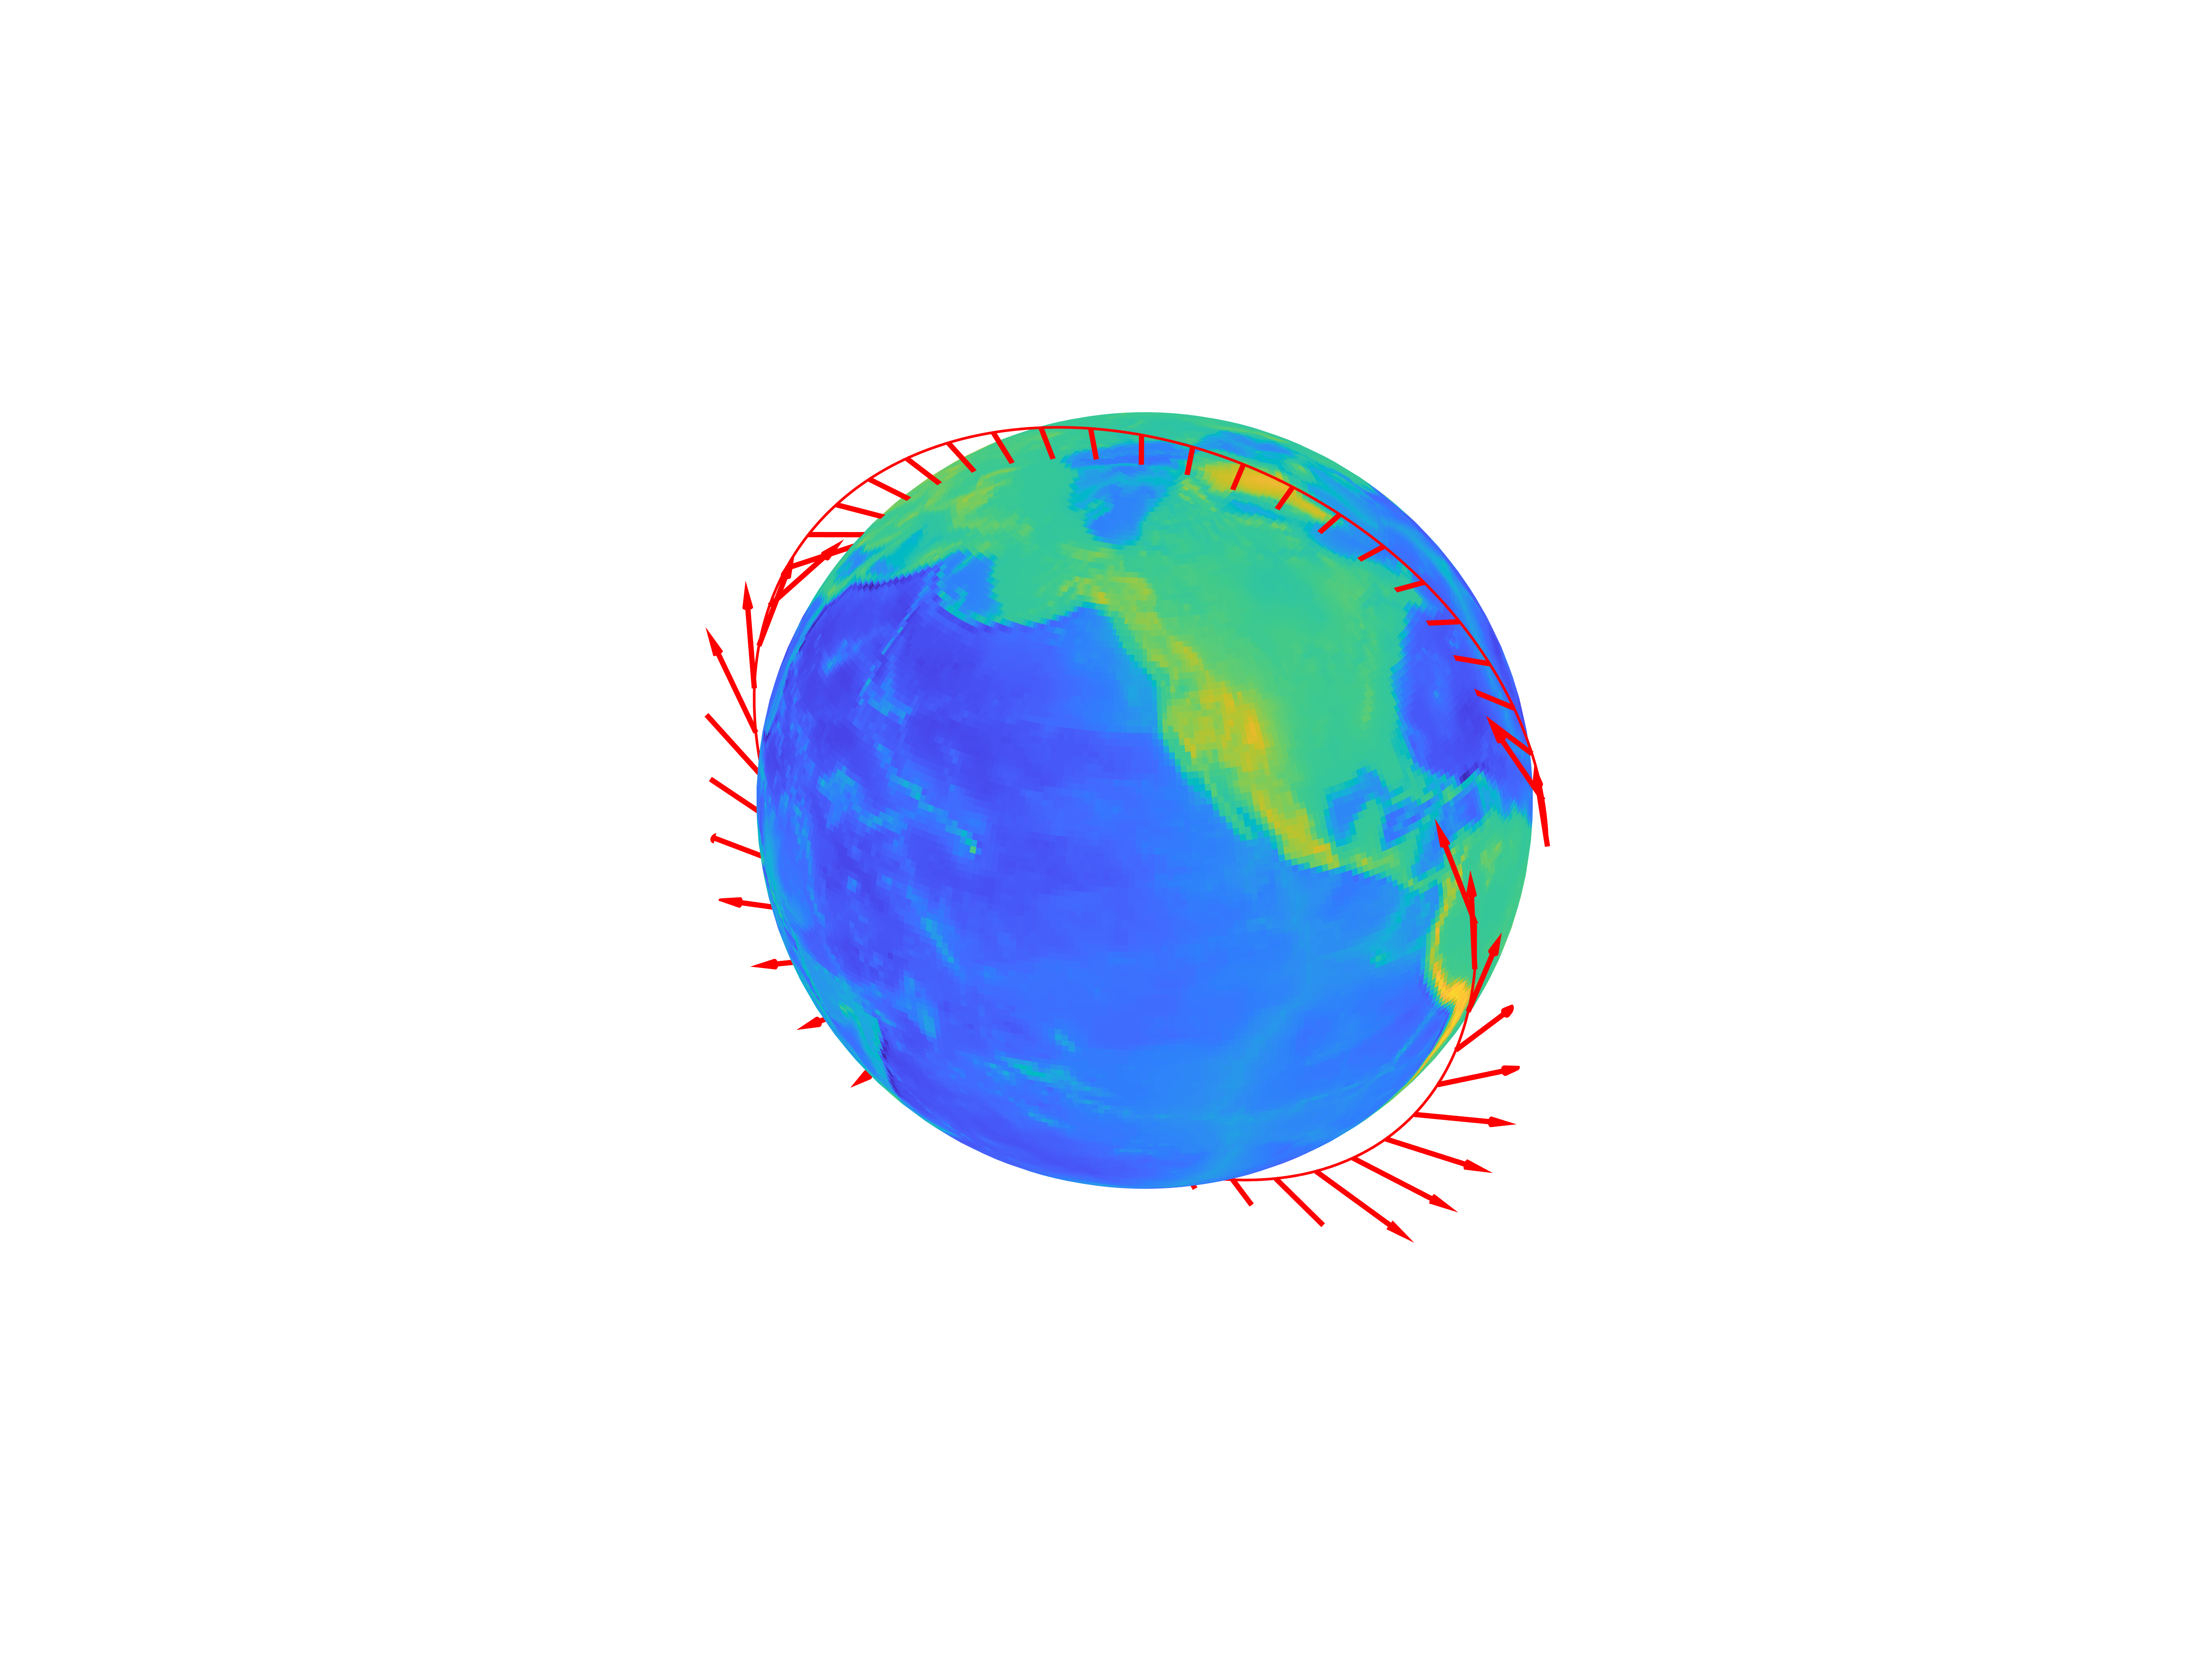
\includegraphics[trim={4.5cm 2.5cm 4cm 2.5cm},clip,width=1\textwidth]{figures/attEst-sim3-mag_90.png}
		\caption{$i=90^\circ$}
	\end{subfigure}
	\caption{Magnetic field on the orbit with different inclinations.}
	\label{fig:attEst-sim3-magnetic}
\end{figure}

Next, the magnetometer measurements are generated as follows. 
Assuming that the simulation begins at the midnight of January 1, 2021, the orbital position in the ECI frame is transformed into the Earth-centered, Earth-fixed (ECEF) frame. 
This is because the Earth magnetic field is fixed to the ECEF frame. 
For the given location with respect to the ECEF frame, the MATLAB function \texttt{wrldmagm} is called to compute the magnetic field.  
This function implements the NOAA World Magnetic Model presented in~\cite{chulliat2020us}. 
Then, the magnetic field is normalized to a unit-vector, which is transformed back to the ECI frame to obtain the true direction of the magnetic field at $t=t_k$, namely $a$ in \eqref{eqn:attEst-update-F}.
Figure \ref{fig:attEst-sim3-magnetic} illustrates the NOAA magnetic field model, where the magnetic field along the selected orbits with respect to the ECEF frame is shown.

The measurement from the magnetometer is assumed to be distributed according to the von Mises--Fisher distribution centered at the true magnetic field resolved in the body-fixed frame, namely $R^Tb\in\Sph^2$.
The concentration parameter $\kappa$ is chosen as $\kappa=200$. 
The average attitude error of the noisy magnetometer measurement is $5.08^\circ$, and it is assumed to be available also at \SI{20}{\hertz}.

Five filters are simulated to estimate the attitude and gyroscope bias of the spacecraft from gyroscope and magnetometer measurements, namely MEKF, two MFGB filters (MFGBA and MFGBU), and two MFGI filters (MFGIA and MFGIU).
The filters are initialized by
\begin{gather*}
	U_0 = \diag{[1,-1,-1]} \quad S_0 = 10I_{3\times 3} \quad V_0 = I_{3\times 3} \\
	\mu_0 = 0_{3\times 1} \quad \Sigma_0 = 0.01^2I_{3\times 3} \quad P_0 = 0_{3\times 3}.
\end{gather*}
The initial attitude estimation is the true attitude rotated by $180^\circ$ about its first body-fixed axis, and the initial bias estimation is off by $\SI{0.01}{\radian\per\second}$ in each axis.

Since there is only one direction measurement available from the magnetometer, the rotation of spacecraft about this reference vector is unobservable if the magnetic field is fixed.
Fortunately, as the spacecraft circles around Earth, the direction of the magnetic field changes at different locations (see Figure \ref{fig:attEst-sim3-magnetic}), and this allows the full attitude to be estimated \cite{grip2011attitude}.
However, since the magnetic field changes very slowly, estimating full attitude still remains very challenging.
Therefore, similar to the previous test, two attitude errors are defined: the full attitude error (FAE) at time $t_k$ is the angle that rotates $(R_{\mathrm{ref}})_k$ to $(R_{\mathrm{est}})_k$, and the partial attitude error (PAE) is the angle between $(R_{\mathrm{ref}})_k^Tb_k$ and $(R_{\mathrm{est}})_k^Tb_k$.
Note that the partial attitude error does not take into account the rotation about the reference vector $b_k$.

\begin{table*}
	\centering
	\caption{Estimation errors with magnetometer measurements \label{tab:attEst-sim3-estError}}
	\small
	\begin{tabular}{c|c|ccccc}
		\multicolumn{2}{c}{} & MEKF & MFGBA & MFGBU & MFGIA & MFGIU \\ \hline
		\multirow{3}{1.2cm}{$i=0^\circ$} & Attitude full error (deg) & 82.0 & 29.4 & 63.4 & 90.1 & 87.0 \\
		& Attitude partial error (deg) & 2.019 & 2.017 & 2.018 & 2.015 & 2.020 \\
		& Bias error (deg/s) & 0.313 & 0.044 & 0.045 & 0.119 & 1.366 \\ \hline
		\multirow{3}{1.2cm}{$i=40^\circ$} & Attitude full error (deg) & 85.0 & 8.7 & 25.7 & 22.0 & 82.9 \\
		& Attitude partial error (deg) & 2.018 & 2.016 & 2.019 & 2.015 & 2.020 \\
		& Bias error (deg/s) & 0.321 & 0.048 & 0.051 & 0.176 & 1.324 \\ \hline
		\multirow{3}{1.2cm}{$i=90^\circ$} & Attitude full error (deg) & 82.8 & 7.2 & 20.5 & 22.8 & 76.8 \\
		& Attitude partial error (deg) & 2.018 & 2.016 & 2.019 & 2.014 & 2.020 \\
		& Bias error (deg/s) & 0.298 & 0.053 & 0.060 & 0.252 & 1.178 \\ \hline
	\end{tabular}
\end{table*}

The estimation errors for the five filters are presented in Table \ref{tab:attEst-sim3-estError} and Figure \ref{fig:attEst-sim3-error-i0} to Figure \ref{fig:attEst-sim3-error-i90}.
In addition, the estimated uncertainties in attitude and bias are presented in Figure \ref{fig:attEst-sim3-error-i0} to Figure \ref{fig:attEst-sim3-error-i90}.
Looking at the bias estimation, the two MFGB based filters are much more accurate than MEKF, though their estimated uncertainties are similar.
Because the bias is represented in the body-fixed frame, MFGB is more appropriate then MFGI to model the attitude-bias correlation.
Therefore, MFGB based filters behave better than MFGI based filters, and this can also be seen from that the MFGB filters have lower bias uncertainty.
In particular, the MFGIU filter has the worst performance in bias estimation.

The partial attitude error is directly related to the magnetometer measurement, and is corrected in every time step.
Hence, it is relatively easy to estimate the partial attitude which is not involved with the rotation about the reference vector.
And as a result, all filters tested are able to estimate partial attitude with equally low estimation error.
Furthermore, the attitude uncertainties in the two axes perpendicular to the reference magnetic field are consistently low for all filters, though there appears to be more fluctuations for MEKF.
Also, the partial attitude error does not depend on the inclination angle $i$ of the orbit.

\begin{figure}
	\centering
	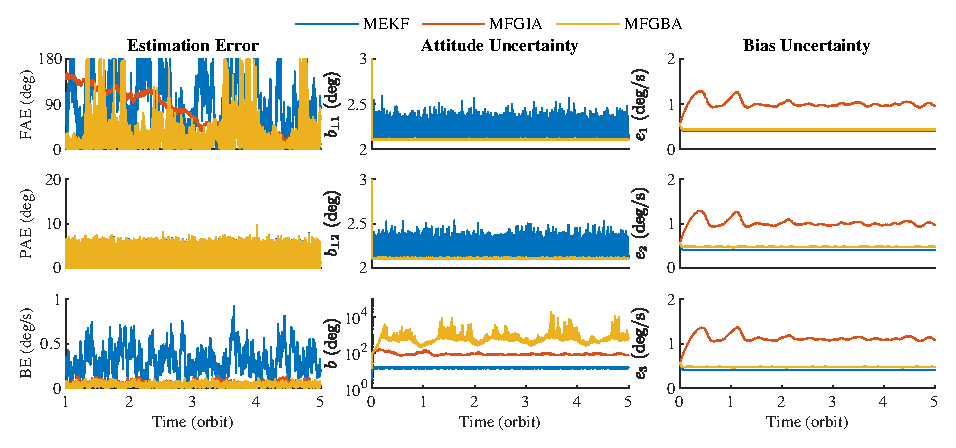
\includegraphics[scale=0.97]{figures/attEst-sim3-error-i0}
	\caption[Estimation error, attitude uncertainty, and bias uncertainty for various attitude filters when $i=0^\circ$.]{Estimation error, attitude uncertainty, and bias uncertainty for various attitude filters when $i=0^\circ$.
		The attitude uncertainty is expressed in the coordinate frame specified by the direction of magnetic field ($b$), and its two perpendicular vectors ($b_{\perp 1}$ and $b_{\perp 2}$).
		The attitude uncertainty for MEKF is given by the square root of the diagonals of its covariance; and that for MFG filters is given by the square root of the diagonals of $(\tr{S}I_{3\times 3}-S)^{-1}$, after transformed into the correct frame.
		The bias uncertainty is expressed in the body-fixed frame, and is given by the square root of the diagonals of the covariance.
		The results for MFG unscented filters are omitted for better readability.}
	\label{fig:attEst-sim3-error-i0}
\end{figure}

\begin{figure}
	\centering
	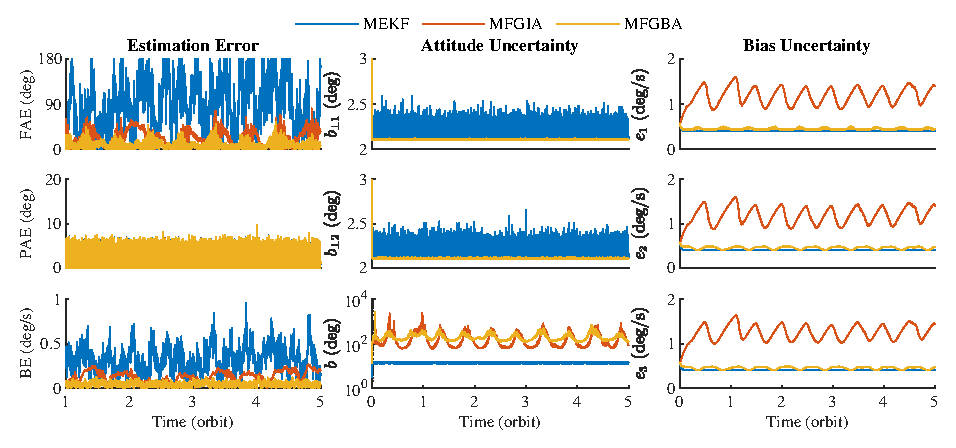
\includegraphics[scale=0.97]{figures/attEst-sim3-error-i40}
	\caption{Estimation error, attitude uncertainty, and bias uncertainty for various attitude filters when $i=40^\circ$.}
	\label{fig:attEst-sim3-error-i40}
\end{figure}

\begin{figure}
	\centering
	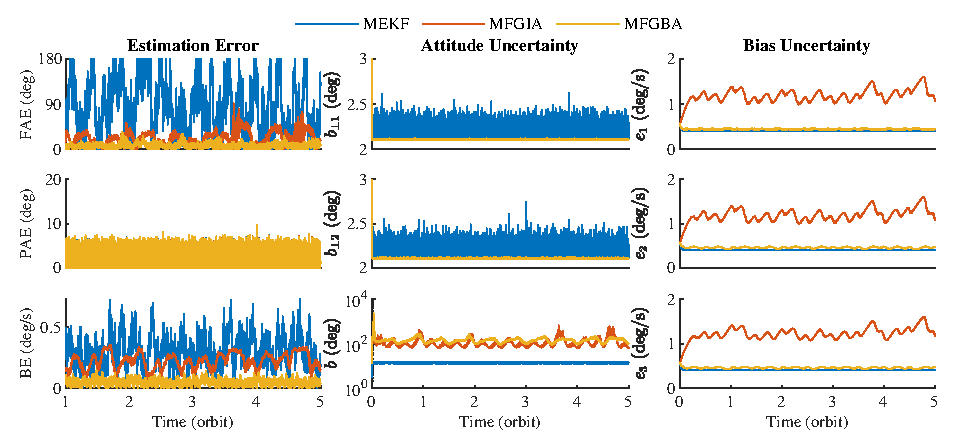
\includegraphics[scale=0.97]{figures/attEst-sim3-error-i90}
	\caption{Estimation error, attitude uncertainty, and bias uncertainty for various attitude filters when $i=90^\circ$.}
	\label{fig:attEst-sim3-error-i90}
\end{figure}

The full attitude is extremely challenging to estimate due to that the direction of magnetic field $b$ changes very slowly.
Among all tested filters, only the MFGB based filters (and in particular MFGBA) are able to give relatively low full attitude error.
Compared with the results in \cite{lee2019spacecraft} where the full attitude can be accurately estimated with a gyroscope and a single magnetometer, the difference here is the inclusion of a non-zero time varying gyroscope bias.
Because there is only one slow-varying reference vector, the integration accuracy of angular velocity from gyroscope is of crucial importance for full attitude estimation.
However, the inclusion of a time varying gyroscope bias deteriorates the integration accuracy very badly.
And therefore, the estimation accuracy of bias has a strong impact on the estimation of full attitude, and this explains why the MFGB based filters have lower full attitude error compared with other filters.
It is surprising that MEKF has the lowest attitude uncertainty in the reference magnetic field direction, nonetheless it is the least accurate in full attitude estimation.
This may reflect that the Gaussian distribution assumed by MEKF cannot properly model the large attitude dispersion due to the wrapping problem.
In addition, the analytical propagation for MFG filters behave consistently better than unscented propagation in full attitude estimation.
Also, because the direction of $b$ changes more quickly as the inclination angle $i$ is increased, the full attitude error also becomes lower.

\subsection{Summary}

In this section, the MFG defined in Chapter \ref{chap:MFG} is used to design an attitude estimator that is able to concurrently estimate the attitude and gyroscope bias.
Because MFG is defined intrinsically on $\SO{3}\times \mathbb{R}^n$, it is able to handle large attitude uncertainty.
Compared with the Gaussian based MEKF, the MFG filter does not show any advantage when the attitude uncertainty is small.
However, for challenging cases with large attitude uncertainty, for example, when the initial attitude is completely wrong, the MFG filters exhibit much faster convergence rate than MEKF.
Also, if there is a degree of freedom that is not properly observed, for example, when a direction measurement is very inaccurate, or when a single reference direction is slowly varying in the inertial frame, the MFG filters have better accuracy than MEKF.
Due to that the gyroscope bias is resolved in the body-fixed frame, the MFGB definition more accurately models the attitude-bias correlation than the MFGI definition.
The advantage of MFGB becomes particularly significant when the attitude uncertainty is highly non-isotropic, which is consistent with the discussion in Chapter \ref{section:MFG-MFGI-MFGB}.

\section{Loosely Coupled IMU-GNSS Integration} \label{section:posEst}

In this section, the attitude estimation problem considered in the previous section is extended into a full inertial navigation problem.
More specifically, it is assumed that an inertial measurement unit (IMU) is attached to a rigid body, which has a gyroscope measuring the angular velocity, and an accelerometer measuring the linear acceleration, both in the body fixed frame.
The linear acceleration can be transformed into the inertial frame using the integrated attitude, and then it can be integrated twice into position after subtracting the gravity component.
It is also assumed that a global navigation satellite system (GNSS) receiver provides position measurements of the rigid body, which are used to correct the attitude and position integrated using the IMU.
Since the pseudorange from GNSS is first converted into position measurements, and then used to correct the inertial navigation estimation, this is usually referred to as loosely coupled IMU-GNSS integration.

The MEKF for attitude estimation can be generalized to deal with this inertial navigation setting \cite{sola2017quaternion}.
However, as discussed in previous sections, it cannot handle large attitude uncertainty due to its inherent Gaussian assumption.
Similar as in attitude estimation, the MFG is used to design a new estimator, which is suitable for large attitude uncertainty.
This is particularly advantageous in some practical problems, for example, when the IMU starts in a building, where the heading direction is usually completely unknown; or when the GNSS receiver cannot receive signal for a long period time, and the uncertainty for inertial navigation accumulates.

The definition of MFG is flexible enough to handle this inertial navigation setting, as its linear part can be arbitrary in $\mathbb{R}^n$.
This makes MFG distinguished from the distribution defined for dual quaternions \cite{li2019geometry,li2020unscented}, where the linear part must be position only.
In this section, the MFG is used to design a Bayesian filter that estimates attitude, gyroscope bias, position, linear velocity, and accelerometer bias concurrently.

\subsection{Problem Formulation}

The IMU kinematic model is formulated in discrete time as follows
\begin{align}
	R_{k+1} &= R_k \expb{ h(\hat{\Omega}_k + \hat{b}_{g,k}) + H_{gu}\Delta W_{gu} }, \label{eqn:posEst-kinematics-attitude} \\
	b_{g,k+1} &= b_{g,k} + H_{gv}\Delta W_{gv}, \label{eqn:posEst-kinematics-gyrobias} \\
	p_{k+1} &= p_k + hv_k, \label{eqn:posEst-kinematics-pos} \\
	v_{k+1} &= v_k - gh + R_k\left( h(a_k+b_{a,k}) + H_{au}\Delta W_{au} \right), \label{eqn:posEst-kinematics-velocity} \\
	b_{a,k+1} &= b_{a,k} + H_{av}\Delta W_{av}, \label{eqn:posEst-kinematics-accebias}
\end{align}
where $R\in\SO{3}$ is the attitude, $x = \big[b_g^T, p^T, v^T, b_a^T\big]^T \in \mathbb{R}^{12}$ are gyroscope bias, position, linear velocity in inertial frame, and accelerometer bias, respectively.
The gravity vector is denoted by $g\in\mathbb{R}^3$.
Next, $\Omega\in\mathbb{R}^3$ is the angular velocity measured by the gyroscope, and $a\in\mathbb{R}^3$ is the linear acceleration measured by the accelerometer, and they are resolved in the body-fixed frame.
The angular velocity measurement is affected by two noises: $H_{gu}\Delta W_{gu}$ is a white noise, and $b_g$ is a random walk bias driven by $H_{gv}\Delta W_{gv}$.
The noises for accelerometer are similar, given by the white noise $H_{au}\Delta W_{au}$, and the bias driven by $H_{av}\Delta W_{av}$.
These noise terms are Gaussian with
\begin{align}
	&H_{gu}\Delta W_{gu} \sim \mathcal{N}(0,hG_{gu}), \quad H_{gv}\Delta W_{gv} \sim \mathcal{N}(0,hG_{gv}), \label{eqn:posEst-gyroNoise} \\
	&H_{au}\Delta W_{au} \sim \mathcal{N}(0,hG_{au}), \quad H_{av}\Delta W_{av} \sim \mathcal{N}(0,hG_{av}),
\end{align}
where $G_{gu} = H_{gu}H_{gu}^T$, $G_{gv} = H_{gv}H_{gv}^T$, $G_{au} = H_{au}H_{au}^T$, $G_{av} = H_{av}H_{av}^T$, and they are independent.
Finally, the subscript $k$ denote the time step, and $h = t_{k+1}-t_k$ is the constant sampling period for any $k$.

It is assumed that the position $p_k$ is measured by a GNSS receiver at time $t_k$, denote by $y_k\in\mathbb{R}^3$.
The measurement noise is Gaussian, i.e.,
\begin{align}
	y_k|p_k = p_k + \mathcal{N}(0,\Sigma_y).
\end{align}
Optionally, the attitude and some reference directions can also be measured as formulated in Chapter \ref{section:attEst-problem}.
Namely, the attitude can be directly measured by $N_a$ sensors as $Z_i$, and the measurement noises follow matrix Fisher distributions with parameters $F_{Z_i}$, for $i=1,\ldots,N_a$.
Also, $N_v$ fixed reference directions $a_j\in\Sph^2$ in inertial frame are measured as $z_j\in\Sph^2$ in the body-fixed frame, and the measurement noises follow von Mises-Fisher distribution with the mean direction $R_t^TB_ja_j$, and concentration parameter $\kappa$, where $R_t\in\SO{3}$ is the true attitude, for $j = 1,\ldots,N_v$.
All measurements at time $t_k$ are denoted by $\mathcal{Z}_k$.

Suppose $(R_0,x_0) = (R_0,b_{g,0},p_0,v_0,b_{a,0})$ at the initial time $t_0$ follow an MFG with $n=12$ and parameters $(\mu_0,\Sigma_0,P_0,U_0,S_0,V_0)$.
Given the IMU measurements $\{\Omega_k,a_k\}_{k=1}^\infty$, and all position, attitude, and direction measurements $\mathcal{Z}_{k=1}^\infty$, the problem is to find the posterior distribution of $(R_k,x_k) | \{\mathcal{Z}_m\}_{m=1}^k$, and approximate it to an MFG with parameters $(\mu_k, \Sigma_k, P_k, U_k, S_k, V_k)$.
Similar to the attitude estimator, two steps are needed.
In the uncertainty propagation step, the posterior distribution $(R_k,x_k) | \{\mathcal{Z}_m\}_{m=1}^k$ is propagated using the IMU kinematic equations \eqref{eqn:posEst-kinematics-attitude}-\eqref{eqn:posEst-kinematics-accebias} to the next time step as $(R_{k+1},x_{k+1}) | \{\mathcal{Z}_m\}_{m=1}^k$.
Next, the propagated distribution is updated by the measurements $\mathcal{Z}_{k+1}$ using Bayes' formula into $(R_{k+1},x_{k+1}) | \{\mathcal{Z}_m\}_{m=1}^{k+1}$.
In the next two subsections, algorithms for these two steps are developed.

\subsection{Uncertainty Propagation} \label{section:posEst-propagation}

Suppose $(R_k,x_k) | \{\mathcal{Z}_m\}_{m=1}^k \sim \mathcal{MG}(\mu_k, \Sigma_k, P_k, U_k, S_k, V_k)$.
In this subsection, the moments of $(R_{k+1},x_{k+1})$ required for the MLE of MFG are calculated using the IMU kinematics equations \eqref{eqn:posEst-kinematics-attitude}-\eqref{eqn:posEst-kinematics-accebias}.
One way of calculating those moments is to propagated deterministically sampled sigma points through the kinematic equations using the unscented transform of MFG, as introduced in Chapter \ref{section:attEst-propagation}.
This approach can be easily generalized to the inertial navigation settings considered in this subsection, and will not be discussed here.
Instead, this subsection calculates approximate analytical expressions of the required moments.

First, because \eqref{eqn:posEst-kinematics-attitude} and \eqref{eqn:posEst-kinematics-gyrobias} are exactly the same as the attitude kinematics considered in \eqref{eqn:attEst-kinematics-att-dist} and \eqref{eqn:attEst-kinematics-bias-dist}, the moment $\expect{R_{k+1}}$ can be calculated using Theorem \ref{thm:attEst-prop-E(R_{k+1})}.
Then $\expect{R_{k+1}}$ is used in the marginal MLE of MFG to obtain the parameters $U_{k+1}$, $S_{k+1}$, and $V_{k+1}$.
Next, define $Q_{k+1} = U_{k+1}^TR_{k+1}V_{k+1}$, and $\nu_{R_{k+1}} = (Q_{k+1}S_{k+1}-S_{k+1}Q_{k+1}^T)^\vee$ for MFGI, or $\nu_{R_{k+1}} = (S_{k+1}Q_{k+1}-Q_{k+1}^TS_{k+1})^\vee$ for MFGB as the intermediate parameters for the MFG at time $t_{k+1}$.
According to Theorem \ref{thm:MFG-MLE-conditional}, $\expect{x_{k+1}}$, $\expect{x_{k+1}\nu_{R_{k+1}}^T}$, $\expect{x_{k+1}x_{k+1}^T}$, and $\expect{\nu_{R_{k+1}}\nu_{R_{k+1}}^T}$ need to be calculated.
Note that $\expect{\nu_{R_{k+1}}\nu_{R_{k+1}}^T}$ is only involved with the gyroscope kinematics \eqref{eqn:posEst-kinematics-attitude} and \eqref{eqn:posEst-kinematics-gyrobias}, so it can be calculated using \eqref{eqn:attEst-prop-EvRvR_{k+1}} in Theorem \ref{thm:attEst-prop-otherMoments}.
In the remainder of this subsection, the calculations for $\expect{x_{k+1}}$, $\expect{x_{k+1}\nu_{R_{k+1}}^T}$, and $\expect{x_{k+1}x_{k+1}^T}$ are developed.

In perpetration for these calculations, the parameters $\mu_k$, $P_k$ and $\Sigma_k$ are written for each component in block form as
\begin{gather} \label{eqn:posEst-prop-blocks}
	\allowdisplaybreaks
	\mu_k = \begin{bmatrix}
		\mu_{b_g,k} \\ \mu_{p,k} \\ \mu_{v,k} \\ \mu_{b_a,k}
	\end{bmatrix}, \qquad
	P_k = \begin{bmatrix}
		P_{b_g,k} \\ P_{p,k} \\ P_{v,k} \\ P_{b_a,k}
	\end{bmatrix}, \qquad
	\Sigma_k = \begin{bmatrix}
		\Sigma_{b_gb_g,k} & \Sigma_{b_gp,k} & \Sigma_{b_gv,k} & \Sigma_{b_gb_a,k} \\
		\Sigma_{pb_g,k} & \Sigma_{pp,k} & \Sigma_{pv,k} & \Sigma_{pb_a,k} \\
		\Sigma_{vb_g,k} & \Sigma_{vp,k} & \Sigma_{vv,k} & \Sigma_{vb_a,k} \\
		\Sigma_{b_ab_g,k} & \Sigma_{b_ap,k} & \Sigma_{b_av,k} & \Sigma_{b_ab_a,k}
	\end{bmatrix}.
\end{gather}
With these, the calculation for $\expect{x_{k+1}}$ is presented in the next theorem.

\begin{theorem} \label{thm:posEst-prop-Ex}
	The moment $\expect{x_{k+1}} = \expect{ b_{g,k+1}^T, p_{k+1}^T, v_{k+1}^T, b_{a,k+1}^T}^T$ are given by
	\begin{align}
		\expect{b_{g,k+1}} &= \expect{b_{g,k}} \\
		\expect{p_{k+1}} &= \expect{p_k} + h\expect{v_k} \\
		\expect{v_{k+1}} &= \expect{v_k} + h\expect{R_k}(a_k+\mu_{b_a,k}) + h\expect{R_kP_{b_a,k}\nu_{R_k}} - gh, \\
		\expect{b_{a,k+1}} &= \expect{b_{a,k}}
	\end{align}
	where $\nu_{R_k} = (Q_kS_k-S_kQ_k^T)^\vee$ for MFGI, or $\nu_{R_k} = (S_kQ_k-Q_k^TS_k)^\vee$ for MFGB, with $Q_k = U_k^TR_kU_k$.
\end{theorem}
\begin{proof}
	The first, second, and fourth equations are immediate from \eqref{eqn:posEst-kinematics-gyrobias}, \eqref{eqn:posEst-kinematics-pos}, and \eqref{eqn:posEst-kinematics-accebias}, because $\Delta W_{gv}$ and $\Delta W_{av}$ have zeros means.
	For the third equation, a similar calculation as \eqref{eqn:MFG-Exx-proof} shows that
	\begin{align*}
		\expect{R_kb_{a,k}} = \expect{R_k}\mu_{b_a,k} + \expect{R_kP_{b_a,k}\nu_{R_k}},
	\end{align*}
	and the desired result is proved.
\end{proof}

The expressions for $\expect{x_{k+1}\nu_{R_{k+1}}^T}$ and $\expect{x_{k+1}x_{k+1}^T}$ are very tedious, and they are relegated to Appendix \ref{app:posEst-prop-moments}.
Note that these two moments, $\expect{\nu_{R_{k+1}}\nu_{R_{k+1}}^T}$, and $\expect{x_{k+1}}$ can be calculated using up to the third order moments of $Q_k\sim\mathcal{M}(S_k)$, with the accuracy of $O(h^2)$.
Then using Theorem \ref{thm:MFG-MLE-conditional}, the parameters $\mu_{k+1}$, $P_{k+1}$ and $\Sigma_{k+1}$ can be obtained.
In summary, the uncertainty $S(R_k,x_k) \sim \mathcal{MG}(\mu_k, \Sigma_k, P_k, U_k, S_k, V_k)$ at time $t_k$ is propagated into $(R_{k+1},x_{k+1}) \sim \mathcal{MG}(\mu_{k+1},\allowbreak \Sigma_{k+1},\allowbreak P_{k+1},\allowbreak U_{k+1},\allowbreak S_{k+1},\allowbreak V_{k+1})$, up to accuracy $O(h^2)$ in moments.
The pseudocode for this uncertainty propagation scheme is summarized in Table \ref{tab:posEst-prop}.

\begin{table}
	\caption{Uncertainty propagation for IMU kinematics}
	\label{tab:posEst-prop}
	\begin{algorithmic}[1]
		\algrule[0.8pt]
		\Procedure{$\mathcal{MG}(t_{k+1}) = $ Uncertainty Propagation}{$\mathcal{MG}(t_k),\Omega_k,a_k$}
		\algrule
		\State Calculate $\expect{R_{k+1}}$ using \eqref{eqn:attEst-prop-E(R_{k+1})} with $\mu_k$, $P_k$, $G_u$ replaced by $\mu_{b_g,k}$, $P_{b_g,k}$ in \eqref{eqn:posEst-prop-blocks}, and $G_{gu}$ in \eqref{eqn:posEst-gyroNoise}, respectively.
		\State Obtain $U_{k+1},S_{k+1},V_{k+1}$ according to Chapter \ref{section:MFG-property} using $\expect{R_{k+1}}$.
		\State Calculate $\expect{\nu_{R_{k+1}}\nu_{R_{k+1}}^T}$ using \eqref{eqn:attEst-prop-EvRvR_{k+1}}, calculate $\expect{x_{k+1}}$, $\expect{x_{k+1}\nu_{R_{k+1}}^T}$ and $\expect{x_{k+1}x_{k+1}^T}$ with Theorem \ref{thm:posEst-prop-Ex}, Theorem \ref{thm:posEst-prop-ExvR}, and Theorem \ref{thm:posEst-prop-Exx}, respectively.
		\State Obtain $\mu_{k+1},\Sigma_{k+1},P_{k+1}$ according to Theorem \ref{thm:MFG-MLE-conditional} using the moments calculated in Step 4.
		\State Set $\mathcal{MG}(t_{k+1}) = \mathcal{MG}(\mu_{k+1},\Sigma_{k+1},P_{k+1},U_{k+1},S_{k+1},V_{k+1})$.
		\EndProcedure
		\algrule[0.8pt]
	\end{algorithmic}
\end{table}

\subsection{Measurement Update} \label{section:posEst-update}

The algorithm for propagating the posterior distribution $(R_k,x_k) | \{\mathcal{Z}_{m}\}_{m=1}^k$ at time $t_k$ into the prior distribution $(R_{k+1},x_{k+1}) | \{\mathcal{Z}_{m}\}_{m=1}^k$ at time $t_{k+1}$ has been introduced in the previous subsection.
In this subsection, the prior distribution $(R_{k+1},x_{k+1}) | \{\mathcal{Z}_{m}\}_{m=1}^k$ is updated into the posterior distribution $(R_{k+1},x_{k+1}) | \{\mathcal{Z}_{m}\}_{m=1}^{k+1}$ at time $t_{k+1}$, with the measurements $\mathcal{Z}_{k+1}$ using Bayes' formula.
Since the update is completed instantaneously at time $t_{k+1}$, the subscript $k+1$ is omitted in this subsection, and the variables relevant to the posterior distribution are denoted by the superscript $+$.

Suppose the prior distribution of $(R,x)$ before measurement update follows MFG with parameters $(\mu,\Sigma,P,U,S,V)$. 
By the Bayes' rule and Theorem 3.2 in \cite{lee2018bayesian}, the posterior density conditioned on all of the available measurements $\mathcal{Z}$ is 
\begin{align} \label{eqn:posEst-update-density}
	&p(R,x\lvert \mathcal{Z}) \propto \etr{ \bigg( F + \sum_{i=1}^{N_a}Z_iF_i^T + \sum_{j=1}^{N_v}\kappa_jB_ja_jz_j^T \bigg)R^T } \nonumber \\
	&\quad \cdot \expb{-\tfrac{1}{2}(x-\mu_c)^T\Sigma_c^{-1}(x-\mu_c)} \cdot \expb{-\tfrac{1}{2}(Hx-y)^T\Sigma_y^{-1}(Hx-y)},
\end{align}
where $H = [0_{3\times 3}, I_{3\times 3}, 0_{3\times 6}]$ selects the position component from $x$, and $F$, $\mu_c$ and $\Sigma_c$ are defined as in Definition \ref{def:MFG} with respect to $\mathcal{MG}(\mu,\Sigma,P,U,S,V)$.
Compared with \eqref{eqn:attEst-update-density} in attitude estimation, \eqref{eqn:posEst-update-density} has an additional term contributed by the position measurement coming from the GNSS receiver.

To deal with this posterior density, it is first shown that \eqref{eqn:posEst-update-density} can be factorized into the marginal component for $R$, and the conditional component for $x|R$.
\begin{lemma} \label{lemma:posEst-update-factor}
	Let $\tilde{F}$ be defined as the $F^+$ in \eqref{eqn:attEst-update-F}, or $\tilde{F} = F$ if there are no attitude or direction measurements.
	Also, define the ``Kalman gain''
	\begin{align}
		K = \Sigma_cH^T(H\Sigma_cH^T + \Sigma_y)^{-1} \in \mathbb{R}^{12\times 3}.
	\end{align}
	Then the posterior density \eqref{eqn:posEst-update-density} can be factorized into two parts:
	\begin{align} \label{eqn:posEst-update-density-factor}
		p(R,x|\mathcal{Z}) = f_R(R) f_{x|R}(x|R),
	\end{align}
	where the marginal part $f_R(R)$ is given by
	\begin{align} \label{eqn:posEst-update-density-R}
		f_R(R) \propto \etr{\tilde{F}R^T} \expb{-\tfrac{1}{2}(H\mu_c-y)^T (\Sigma_y+H\Sigma_cH^T)^{-1} (H\mu_c-y)},
	\end{align}
	and the conditional part $f(x|R)$ is given by
	\begin{align} \label{eqn:posEst-update-density-x|R}
		f_{x|R}(x|R) \propto \expb{-\tfrac{1}{2} \big(x-(I-KH)\mu_c-Ky\big)^T \big((I-KH)\Sigma_c\big)^{-1} \big(x-(I-KH)\mu_c-Ky\big)},
	\end{align}
	where $I$ is abbreviated for $I_{12\times 12}$.
\end{lemma}
\begin{proof}
	Using a similar technique that is used to prove the linear Kalman filter, and the Woodbury matrix identity \cite{petersen2008matrix}, it can be proved that
	\begin{align*}
		&\expb{-\tfrac{1}{2}(x-\mu_c)^T\Sigma_c^{-1}(x-\mu_c)} \cdot \expb{-\tfrac{1}{2}(Hx-y)^T\Sigma_y^{-1}(Hx-y)} \\
		= &\expb{-\tfrac{1}{2} \big(x-(I-KH)\mu_c-Ky\big)^T \big((I-KH)\Sigma_c\big)^{-1} \big(x-(I-KH)\mu_c-Ky\big)} \\
		&\qquad \cdot \expb{-\tfrac{1}{2}(H\mu_c-y)^T (\Sigma_y+H\Sigma_cH^T)^{-1} (H\mu_c-y)},
	\end{align*}
	which gives the desired \eqref{eqn:posEst-update-density-factor}.
\end{proof}

Note that the marginal part $f_R(R)$ does not depend on $x$, so according to the marginal-conditional MLE of MFG, the first step is to approximate $f_R(R)$ into the density function of a matrix Fisher distribution.
Since the $\mu_c$ is linear in $R$, $f_R(R)$ has quadratic terms of $R$ in its exponent, making the expectation $\expect{R}$ corresponding to $f_R(R)$ impractical to be calculated directly from the density function.
Instead, $\expect{R}$ is approximated using the unscented transform of matrix Fisher distribution \cite{gilitschenski2015unscented,lee2018bayesian} \footnote{The unscented transform in \cite{gilitschenski2015unscented} is developed for the Bingham distribution, and it can be converted to the matrix Fisher distribution using Theorem \ref{thm:Bh2MF}}.
The idea is that the weighted sigma points $\{R_i,w_i\}_{i=1}^7$ are selected from $\mathcal{M}(\tilde{F})$, corresponding to the first part of \eqref{eqn:posEst-update-density-R}.
The weights are reweighed by the second part of \eqref{eqn:posEst-update-density-R} as
\begin{align} \label{eqn:posEst-update-sigmapoints}
	w_i^+ = w_i \expb{-\tfrac{1}{2}(H\mu_{c,i}-y)^T (\Sigma_y+H\Sigma_cH^T)^{-1} (H\mu_{c,i}-y)},
\end{align}
where $\mu_{c,i}$ are calculated using $R_i$ as in \eqref{eqn:MFG-Miuc}, for $i=1,\dots,7$.
Then the moment $\expect{R}$ is approximated using these reweighed sigma points as $\sum_{i=1}^7 w_i^+R_i$ after normalization.
This update procedure comes from particle filters \cite{arulampalam2002tutorial} where the deterministic sigma points are replaced by the randomly sampled particles, and has been widely applied in Bayesian filters with nonlinear measurement functions \cite{kurz2016recursive}.

However, as noted in \cite{kurz2016recursive}, the approximation of $\expect{R}$ using this technique can sometimes degenerate, i.e., some or all of $w_i^+$ can be close to zero due to large discrepancies between $H\mu_{c,i}$ and $y$.
To overcome this problem, the ``progressive update'' developed in \cite{hanebeck2013pgf} is used here, which has been applied to several stochastic filters \cite{huang2015gaussian,kurz2014nonlinear,li2021progressive}.
Denote the second term on the right hand side of \eqref{eqn:posEst-update-density-R} as $f_m(R)$.
The idea of progressive update is that instead of multiplying the full $f_m(R_i)$ to the weights, $f_m(R)$ is decomposed into several parts as
\begin{align*}
	f_m(R) = f_m(R)^{\lambda_1} f_m(R)^{\lambda_2} \cdots f_m(R)^{\lambda_l},
\end{align*}
where $\sum_{i=1}^l \lambda_i = 1$, and $\lambda_i>0$.
In the first step, $w_i$ is reweighed by
\begin{align*}
	w_i^1 = w_i f_m(R_i)^{\lambda_1},
\end{align*}
for $i=1,\ldots,7$, so that no $w_i^1$ is close to zero if $\lambda_1$ is properly chosen.
The criterion for proper $\{w_i^1\}$ is that $\tfrac{\min\{f_m(R_i)^{\lambda_1}\}}{\max\{f_m(R_i)^{\lambda_1}\}} \geq \tau$ for some $\tau \in (0,1)$, i.e., the smallest and largest $w_i^1$ are not different by too much.
If this is satisfied for $\lambda_1 = 1$, then the process is finished, and $w_i^+ = w_i^1$ for $i=1,\ldots,7$ are used to calculate $\expect{R}$, which is matched to a matrix Fisher distribution with parameter $F^1$ using the MLE in Chapter \ref{section:MF-MF}.

Otherwise, $\lambda_1$ is chosen as $\log\tau / \log\left( \tfrac{\min\{f_m(R_i)\}}{\max\{f_m(R_i)\}} \right)$, so $\tfrac{\min\{f_m(R_i)^{\lambda_1}\}}{\max\{f_m(R_i)^{\lambda_1}\}} = \tau$.
Then the reweighed sigma points $\{R_i, w_i^1\}$ are used to calculate the expectation $\sum_{i=1}^7 w_i^1 R_i$, which is matched to a matrix Fisher distribution with the parameter $F^1$.
Next, in the second step, a new set of sigma points $\{R_i,w_i\}_{i=1}^7$ are selected from $\mathcal{M}(F^1)$, and they are reweighed using $f_m(R_i)^{1-\lambda_1}$.
The new weights are tested again whether $\tfrac{\min\{f_m(R_i)^{1-\lambda_1}\}}{\max\{f_m(R_i)^{1-\lambda_1}\}} \geq \tau$.
If this is satisfied, the process is finished, otherwise this is continued.
Finally, the last $F^l$ is set as the parameter $F^+$ of the matrix Fisher distribution that approximates \eqref{eqn:posEst-update-density-R}.

This progressive update scheme for the posterior parameter $F^+$ is summarized in Table \ref{tab:posEst-update-att}.
It should be noted that if the unscented transform in \cite{lee2018bayesian} is used to select sigma points in step 12, the moment $\expect{R}$ must be first matched to a matrix Fisher distribution.
Whereas if the unscented transform in \cite{gilitschenski2015unscented} is used, $\expect{R}$ can be directly used and there is no need to solve \eqref{eqn:MF-S2D} which is very computationally demanding.

\begin{table}
	\caption{Attitude progressive update}
	\label{tab:posEst-update-att}
	\begin{algorithmic}[1]
		\algrule[0.8pt]
		\Procedure{$F^+ = $ Attitude Update}{$F^-$, $Z$, $z$, $y$}
		\algrule
		\State Compute $\tilde{F} = F^+$ from \eqref{eqn:attEst-update-F}.
		\State Select sigma points \cite{gilitschenski2015unscented,lee2018bayesian} from $\mathcal{M}(\tilde{F})$ as $\{R_i,w_i\}_{i=1}^7$.
		\State Let $\lambda = 1$.
		\While{$\lambda > 0$}
		\State For $i=1,\ldots,7$, calculate $f_m(R_i)^\lambda$, where $f_m(R)$ is the second term on the right hand side of \eqref{eqn:posEst-update-density-R}.
		\If{$\min\{f_m(R_i)^{\lambda}\} / \max\{f_m(R_i)^{\lambda}\} < \tau$}
		\State Let $\alpha = \log\tau / \log\left( \tfrac{\min\{f_m(R_i)\}}{\max\{f_m(R_i)\}} \right)$.
		\State For $i=1,\ldots,7$, calculate $f_m(R_i)^\alpha$.
		\State For $i=1,\ldots,7$, update the weights as $w_i^+ = w_i f_m(R_i)^\alpha$.
		\State Normalize the weights as $w_i^+ = w_i^+/\sum_{i=1}^7 w_i^+$.
		\State Calculate $\expect{R} = \sum_{i=1}^7 w_i^+ R_i$.
		\State Select sigma points $\{R_i,w_i\}_{i=1}^7$ from the matrix Fisher distribution that has the moment $\expect{R}$.
		\State Set $\lambda = \lambda-\alpha$.
		\Else
		\State Set $\lambda = 0$.
		\EndIf
		\EndWhile
		\State For $i=1,\ldots,7$, update the weights as $w_i^+ = w_i f_m(R_i)^\lambda$.
		\State Normalize the weights as $w_i^+ = w_i^+/\sum_{i=1}^7 w_i^+$.
		\State Calculate $\expect{R} = \sum_{i=1}^7 w_i^+ R_i$.
		\State Obtain $F^+$ using the MLE of matrix Fisher distribution in Chapter \ref{section:MF-MF} from $\expect{R}$.
		\EndProcedure
		\algrule[0.8pt]
	\end{algorithmic}
\end{table}

Next, the conditional part of \eqref{eqn:posEst-update-density-factor}, i.e., the $f_{x|R}(x|R)$ in \eqref{eqn:posEst-update-density-x|R} is considered.
As $f_R(R)$ in \eqref{eqn:posEst-update-density-R} has been approximated by the density function of the matrix Fisher distribution with parameter $F^+$, the posterior density \eqref{eqn:posEst-update-density-factor} is now approximated by
\begin{align} \label{eqn:posEst-update-density-approx}
	p(R,x|\mathcal{Z}) \approx c \cdot \etr{F^+R^T} f_{x|R}(x|R),
\end{align}
where $c$ is a constant independent of $(R,x)$.
Let $F^+ = U^+S^+(V^+)^T$ be its proper singular value decomposition, define $\nu_R^+ = (Q^+S^+ - S^+(Q^+)^T)^\vee$ for MFGI, or $\nu_R^+ = (S^+Q^+ - (Q^+)^TS^+)^\vee$ for MFGB, with $Q^+ = (U^+)^TS^+V^+$.
Then to match the above density function to an MFG, the conditional MLE in Theorem \ref{thm:MFG-MLE-conditional} needs to be used, which requires the moments $\expect{x|\mathcal{Z}}$, $\expect{x(\mu_R^+)^T|\mathcal{Z}}$, and $\expect{xx^T|\mathcal{Z}}$ to be calculated.
These expectations are evaluated with respect to \eqref{eqn:posEst-update-density-approx}, and are calculated in the next theorem.

\begin{theorem} \label{thm:posEst-update-moments}
	The moments $\expect{x|\mathcal{Z}}$ and $\expect{x(\nu_R^+)^T|\mathcal{Z}}$ with respect to the density function \eqref{eqn:posEst-update-density-approx} are given by
	\begin{align}
		&\expect{x|\mathcal{Z}} = (I-KH)(\mu+P\expect{\nu_R|\mathcal{Z}}) + Ky, \\
		&\expect{x(\nu_R^+)^T|\mathcal{Z}} = (I-KH)P\expect{\nu_R(\nu_R^+)^T|\mathcal{Z}}.
	\end{align}
	And the moment $\expect{xx^T|\mathcal{Z}}$ is
	\begin{align}
		\expect{xx^T|\mathcal{Z}} &= (I-KH)\Sigma_c + (I-KH) \Big( \mu\mu^T + \mu\expect{\nu_R|\mathcal{Z}}^TP^T + P\expect{\nu_R|\mathcal{Z}}\mu^T \nonumber \\
		&\qquad + P\expect{\nu_R\nu_R^T|\mathcal{Z}}P^T \Big) (I-KH)^T + (I-KH)\left( \mu + P\expect{\nu_R|\mathcal{Z}} \right)y^TK^T \nonumber \\
		&\qquad + Ky\left(\mu^T + \expect{\nu_R^T|\mathcal{Z}}P^T\right)(I-KH)^T + Kyy^TK^T.
	\end{align}
	In the above equations, $I$ is abbreviated for $I_{12\times 12}$.
	Also, $\expect{\nu_R|\mathcal{Z}}$, $\expect{\nu_R\nu_R^T|\mathcal{Z}}$, and $\expect{\nu_R(\nu_R^+)^T|\mathcal{Z}}$ are calculated the same as in Theorem \ref{thm:attEst-update-moments}.
\end{theorem}
\begin{proof}
	These equations are obtained by first integrating against the Gaussian density $f_{x|R}(x|R)$ in \eqref{eqn:posEst-update-density-approx}, as in \eqref{eqn:MFG-Exx-proof}, and noting that $\expect{\nu_R^+|\mathcal{Z}} = 0$.
\end{proof}

Using $\expect{x|\mathcal{Z}}$, $\expect{x(\mu_R^+)^T|\mathcal{Z}}$, and $\expect{xx^T|\mathcal{Z}}$ in the above theorem, the conditional MLE of MFG can be used to obtain the posterior parameters $\mu^+$, $P^+$, and $\Sigma^+$.
In summary, this subsection develops an algorithm to update the prior distribution $(R,x) \sim \mathcal{MG}(\mu,\allowbreak \Sigma,\allowbreak P,\allowbreak U,\allowbreak S,\allowbreak V)$ into the posterior distribution $(R,x)|\mathcal{Z} \sim \mathcal{MG}(\mu^+,\allowbreak \Sigma^+,\allowbreak P^+,\allowbreak U^+,\allowbreak S^+,\allowbreak V^+)$ conditioned by the measurement $\mathcal{Z}$.
Together with the uncertainty propagation scheme in Chapter \ref{section:posEst-propagation}, they constitute a recursive Bayesian filter for a loosely coupled IMU-GNSS system that simultaneously estimates attitude, linear velocity, position, gyroscope bias and accelerometer bias.
The pseudocode is summarized in Table \ref{tab:posEst-filter}.

\begin{table}
	\caption{Bayesian estimation for IMU-GNSS navigation \label{tab:posEst-filter}}
	\begin{algorithmic}[1]
		\algrule[0.8pt]
		\Procedure{Estimation}{$\mathcal{MG}(t_0),\Omega(t),a(t),\mathcal{Z}(t)$}
		\algrule
		\State Let $k=0$.
		\Repeat
		\State $\mathcal{MG}(t_{k+1})$ = Uncertainty Propagation($\mathcal{MG}(t_k)$,$\Omega(t_k)$,$a(t_k)$) in Table \ref{tab:posEst-prop}.
		\State $k=k+1$.
		\Until $y(t_{k+1})$ ia available
		\State $\mathcal{MG}(t_{k+1})$ = Measurement Update($\mathcal{MG}(t_{k+1})$,$Z(t_{k+1})$,$z(t_{k+1})$,$y(t_{k+1})$).
		\State Obtain the estimates as $R(t_{k+1})=U_{k+1}V_{k+1}^T$, $x(t_{k+1})=\mu_{k+1}$ for $\mathcal{MG}(t_{k+1})$.
		\State \textbf{go to} step 3.
		\EndProcedure
		\algrule
		\Procedure{$\mathcal{MG}^+$ = Measurement Update}{$\mathcal{MG}^-$,$Z$,$z$,$y$}
		\State $F^+$ = Attitude Update($U^-S^-(V^-)^T$,$Z$,$z$,$y$) in Table \ref{tab:posEst-update-att}.
		\State Let the pSVD of $F^+$ be $F^+ = U^+S^+(V^+)^T$.
		\State Calculate the moments of the posterior density in Theorem \ref{thm:posEst-update-moments}.
		\State Obtain $\mu^+,\Sigma^+,P^+$ according to Theorem \ref{thm:MFG-MLE-conditional}.
		\State Set $\mathcal{MG}^+ = \mathcal{MG}(\mu^+,\Sigma^+,P^+,U^+,S^+,V^+)$.
		\EndProcedure
		\algrule[0.8pt]
	\end{algorithmic}
\end{table}

\subsection{Numerical Simulations}

In this subsection, the recursive Bayesian filter developed for IMU-GNSS navigation using MFG is compared with the filter in \cite{sola2017quaternion} which is based on MEKF through numerical simulations.
In this simulation study, a vehicle is assumed to move in a circle with radius $\SI{20}{\meter}$ on the ground.
The speed of the vehicle fluctuates from $\SI{0}{\meter/\second}$ to $\SI{10}{\meter/\second}$ as a sinusoidal function with the frequency at $\SI{0.2}{\hertz}$.
The resulting average free acceleration is $\SI{4.88}{\meter/\second\squared}$.
The vehicle simultaneously undergoes a rotational motion where the three Euler angles (body-fixed 3-2-1) follow sinusoidal functions with the frequency at \SI{0.35}{\hertz}, and the amplitudes of $\pi$, $\pi/2$ and $\pi$, respectively.
The corresponding average angular speed is \SI{6.17}{\radian/\second}.

The IMU is assumed to be sampled at $\SI{200}{\hertz}$.
The gyroscope white noise is isotropic with $\sigma_{gu} = \SI{1}{\deg/\sqrt{\second}}$, i.e., $H_{gu} = \sigma_{gu}I_{3\times 3}$ in \eqref{eqn:posEst-kinematics-attitude}.
And its bias random walk noise is isotropic with $\sigma_{gv} = \SI{50}{\deg/\hour/\sqrt{\second}}$, i.e., $H_{gv} = \sigma_{gv}I_{3\times 3}$ in \eqref{eqn:posEst-kinematics-gyrobias}.
Similarly, the accelerometer white noise is isotropic with $\sigma_{au} = \SI{0.01}{\meter/\second/\sqrt{\second}}$, and its bias random walk noise is $\sigma_{av} = \SI{0.333}{\meter/\second\squared/\sqrt{\hour}}$, i.e., $H_{au} = \sigma_{au}I_{3\times 3}$ in \eqref{eqn:posEst-kinematics-velocity} and $H_{av} = \sigma_{av}I_{3\times 3}$ in \eqref{eqn:posEst-kinematics-accebias}.
The GNSS receiver is assumed to be sampled at $\SI{10}{\hertz}$, with the noise $\Sigma_y = \sigma_y^2I_{3\times 3}$, where $\sigma_y = \SI{1}{\meter}$.
There are no attitude or direction measurements.

The initial position is given as the first measurement from the GNSS receiver, and its uncertainty is set the same as $\Sigma_y$.
The initial velocity, gyroscope and accelerometer biases are assumed to be zero, with the uncertainty $0.01^2I_{3\times 3}$.
Two cases for the initial attitude are tested.
In the first case, the initial attitude is randomly chosen from $R_t(0)\expb{\delta\hat{\theta}}$, where $\delta\theta\sim\mathcal{N}(0,0.1^2I_{3\times 3})$.
The initial attitude uncertainty for MEKF is set as $0.1^2I_{3\times 3}$, and for the MFG filters is $S_0 = 50I_{3\times 3}$.
This indicates an initial condition with relatively small attitude uncertainty.
To challenge the filters with large uncertainty, in the second case, it is assumed that the gravity direction is given by the first accelerometer measurement, assuming zero free acceleration.
And the rotation around gravity is set as the true direction rotated by $\SI{180}{\deg}$, indicating a completely wrong heading.
This scenario is frequently encountered in practical navigation problems when the initial heading direction cannot be estimated, for example in a building where the magnetometer reading is unreliable.
The initial attitude uncertainties in the directions perpendicular to gravity, i.e., $s_1$ for MFG, and the first two diagonal entries of the covariance matrix for MEKF, are determined from the accuracy of the accelerometer.
And the initial uncertainty in the heading direction is set for MFG as $s_2 = s_3 = 0$, and for MEKF as $1000$ for the third diagonal entry of the covariance matrix.
All initial correlation terms are set as zero.

The simulation is run for 60 seconds.
A hundred Monte Carlo runs with respect to the random noises are carried out for each initial attitude condition.
The estimation error for attitude is defined as the angle needed to rotate the estimated attitude to the true attitude, and for other Euclidean quantities are defined as the Euclidean distance.
The errors are first averaged across all time steps in a single simulation, and further averaged across 100 simulations.
Paired t-test is conducted between MEKF and the two MFG filters, with the significance level set as $\alpha=0.001$, to indicate any statistical significance.

\begin{table*}
	\centering
	\caption{Estimation errors with small initial attitude error $\pm$ S.D. ($p$-value)}
	\label{tab:posEst-error-1}
	\small
	\begin{tabular}{c|ccc}
		\hline\hline
		 & MEKF & MFGI & MFGB \\ \hline
		attitude error ($\SI{}{\deg}$) & 3.21$\pm$0.43 & 3.23$\pm$0.39 (0.207) & 3.24$\pm$0.38 (0.166) \\ \hline
		gyroscope bias error ($\SI{}{\deg/\second}$) & 0.37$\pm$0.11 & 0.36$\pm$0.11 (0.777) & 0.36$\pm$0.11 (0.860) \\ \hline
		position error ($\SI{}{\meter}$) & 0.585$\pm$0.034 & 0.586$\pm$0.033 (0.163) & 0.586$\pm$0.033 (0.259) \\ \hline
		velocity error ($\SI{}{\meter/\second}$) & 0.568$\pm$0.039 & 0.570$\pm$0.036 (0.169) & 0.569$\pm$0.036 (0.233) \\ \hline
		accelerometer bias error ($\SI{}{\meter/\second\squared}$) & 0.045$\pm$0.016 & 0.045$\pm$0.015 (0.777) & 0.045$\pm$0.015 (0.793) \\ \hline\hline
	\end{tabular}
\end{table*}

\begin{table*}
	\centering
	\caption{Estimation errors with large initial attitude error $\pm$ S.D. ($p$-value)}
	\label{tab:posEst-error-2}
	\small
	\begin{tabular}{c|ccc}
		\hline\hline
		& MEKF & MFGI & MFGB \\ \hline
		attitude error ($\SI{}{\deg}$) & 23.3$\pm$21.7 & 6.91$\pm$0.95 (<0.001) & 7.23$\pm$1.25 (<0.001) \\ \hline
		gyroscope bias error ($\SI{}{\deg/\second}$) & 1.63$\pm$1.31 & 0.36$\pm$0.12 (<0.001) & 0.36$\pm$0.11 (<0.001) \\ \hline
		position error ($\SI{}{\meter}$) & 1.54$\pm$0.99 & 0.63$\pm$0.04 (<0.001) & 0.63$\pm$0.04 (<0.001) \\ \hline
		velocity error ($\SI{}{\meter/\second}$) & 2.23$\pm$1.59 & 0.72$\pm$0.06 (<0.001) & 0.73$\pm$0.08 (<0.001) \\ \hline
		accelerometer bias error ($\SI{}{\meter/\second\squared}$) & 0.074$\pm$0.043 & 0.044$\pm$0.015 (<0.001) & 0.044$\pm$0.015 (<0.001) \\ \hline\hline
	\end{tabular}
\end{table*}

The results for the case with small attitude error is summarized in Table \ref{tab:posEst-error-1}.
It is shown that the MEKF and two MFG filters have negligible differences in all estimations, and no statistical significance is found.
This result is consistent with the small uncertainty in attitude estimation as presented in Table \ref{tab:attEst-sim1-error}, and is expected because the MFG with small uncertainty can be well approximated by a Gaussian distribution.

Next, the result with completely wrong initial heading direction is shown in Table \ref{tab:posEst-error-2}.
In the presence of large initial attitude uncertainty, the two MFG filters have significantly better accuracy in all estimations than MEKF.
The error trajectory of a single simulation is presented in Figure \ref{fig:posEst-error}.
It is seen that the major advantage of MFG filters is that the attitude error converges much faster than MEKF.
Although the estimation errors for other quantities are initially small for all filters, the wrong estimation of attitude makes the error grow very large for MEKF later.
This is because the integrated velocity and position from \eqref{eqn:posEst-kinematics-velocity} and \eqref{eqn:posEst-kinematics-pos} contains large error due to the inaccuracy of attitude, but the MEKF still maintains small variance of these integrated values, giving falsely high confidence to them in the measurement update step.

\begin{figure}
	\centering
	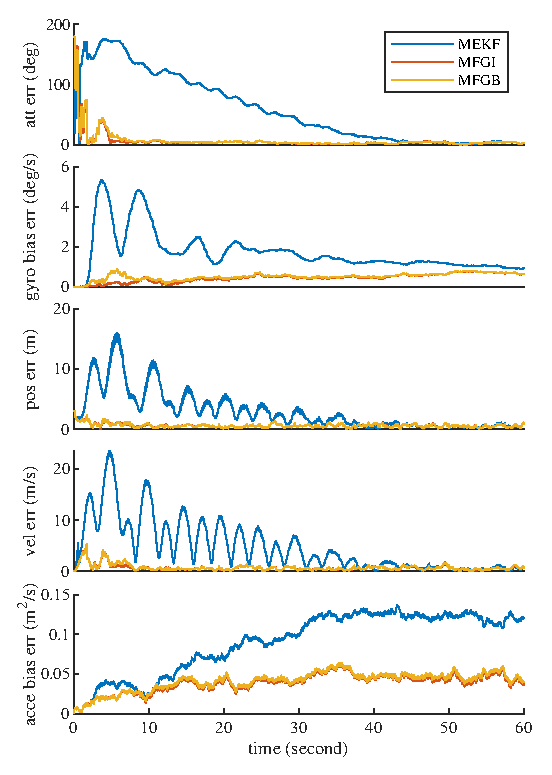
\includegraphics[scale=1.2]{figures/posEst-error}
	\caption{Estimation errors with large initial attitude error.}
	\label{fig:posEst-error}
\end{figure}

\begin{figure}
	\centering
	\begin{subfigure}{\textwidth}
		\centering
		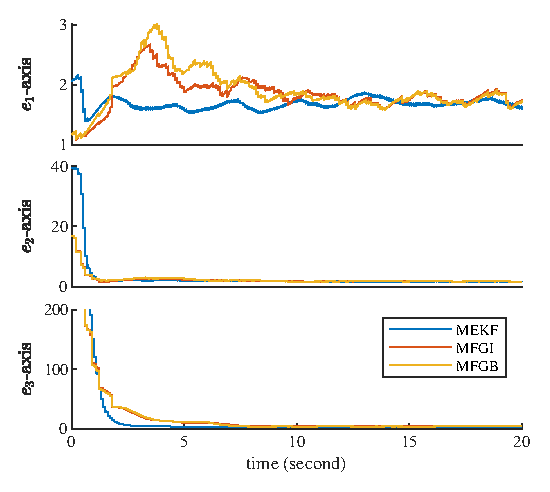
\includegraphics[scale=1.15]{figures/posEst-std-att}
		\caption{Attitude Uncertainty}
		\label{fig:posEst-std-att}
	\end{subfigure}
	\begin{subfigure}{\textwidth}
		\centering
		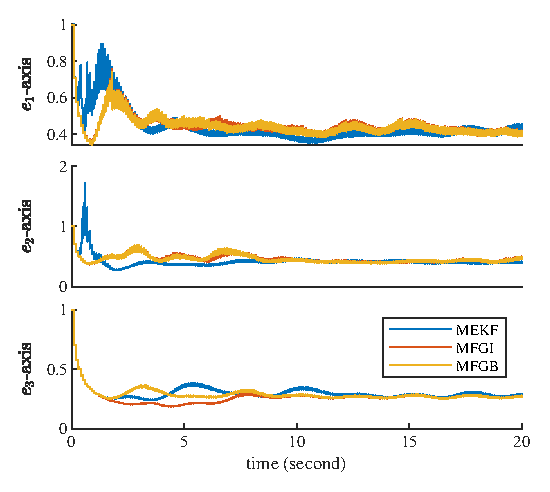
\includegraphics[scale=1.15]{figures/posEst-std-pos}
		\caption{Position Uncertainty}
		\label{fig:posEst-std-pos}
	\end{subfigure}
	\caption[Estimation standard deviations with large initial error.]{Estimation standard deviations with large initial error.
		The attitude standard deviation for MFG is the square root of the diagonals of $U(\tr{S}I_{3\times 3}-S)^{-1}U^T$, and for MEKF is the square root of the diagonals of the covariance matrix transformed into the inertial frame using the estimated attitude.
		And the position standard deviation is the square root of the corresponding entry in the covariance matrix.}
	\label{fig:posEst-std}
\end{figure}

This is more clearly seen in Figure \ref{fig:posEst-std}, where the estimated standard deviations of the attitude and position are shown.
It is seen that although the MEKF has very large attitude error, its uncertainty is on the same level of MFG filters.
Looking at the attitude standard deviation around the gravity direction (the third row in Figure \ref{fig:posEst-std-att}), it converges exponentially for MEKF, which is typical for an EKF.
On the other hand, it converges slower for the MFG filters, possibly indicating that MFG has better accuracy in modeling large attitude uncertainty, as the attitude dose not converge very fast as indicated in Figure \ref{fig:posEst-error}.
Note that in this IMU-GNSS navigation simulation, the attitude is not directly observed, and it is corrected by its correlation with the position.
This suggests that the MFG not only has better accuracy in attitude uncertainty, but also in the correlation between attitude and position, when the attitude uncertainty is large.

\section{Visual-Inertial Odometry} \label{section:VIO}

In this section, the same inertial navigation setting as in the previous section is studied.
But instead of using direct position measurements from GNSS receivers, it is assumed that the 3D coordinates of some unknown features or known landmarks in the inertial frame are measured by cameras.
This is usually referred to as a visual-inertial system.
In this section, two cases are distinguished: (i) if the features captured by the camera are landmarks whose 3D coordinates are known in advance (possibly with noises), it is referred to as visual-inertial \textit{navigation};
(ii) if instead there is no prior information of the features, it is referred to as visual-inertial \textit{odometry}.
To simplify analysis, instead of studying projection measurements on the image plane, it is assumed that the camera is in RGB-D or stereo configuration, so that the location, i.e., the 3D coordinates in the inertial frame, of the feature or landmark has already been triangulated.
And the measured location is directly used to correct any integration errors from the inertial system.

As reviewed in Chapter \ref{section:intro-review-VIO}, the VIO algorithms can be roughly classified into two categories: filtering and optimization.
The optimization based VIO algorithms have achieved better accuracy, but it is usually more computationally demanding.
This section will primarily focus on the filtering approach.
The reason is that in the optimization method, the uncertainty of pose is not modeled, and the uncertainty for pre-integrated IMU pose is only for a short period of time which is very accurate, so the MFG which is designed to model large uncertainty is not very useful.
On the other hand, the filtering method has to model the uncertainty of pose directly, where large uncertainty is frequently encountered.

More specifically, this section will first study a general problem of estimating a pose and its uncertainty that aligns two 3D point sets with known correspondences.
This is usually one of the steps in point cloud registration \cite{huang2021comprehensive}.
It is first assumed that the 3D coordinates of one point set are perfectly known (map), and the other point set has noises (measurement).
Then based on the proposed algorithm, noises for the map point set are also considered.
The uncertainty of the estimated pose is modeled by MFG to deal with possibly large attitude uncertainties.
Together with the uncertainty propagation method proposed in Chapter \ref{section:posEst-propagation}, these constitute a visual-inertial navigation algorithm when known landmarks in the inertial frame are measured.
Finally, this algorithm is extended to a visual-inertial odometry algorithm where unknown features are measured without any prior information.

\subsection{Pose Estimation Without Map Uncertainty} \label{section:VIO-pose}

First, this subsection studies the problem of finding the pose that aligns two point sets using MFG.
Suppose the coordinates of landmarks in the inertial frame are given as $\{p_i\}_{i=1}^N$.
These are measured by a camera in the body-fixed frame as $\{p'_i\}_{i=1}^N$.
It is assumed that the correspondences are known, i.e., $p'_i$ is the measurement of $p_i$, for $i = 1,\ldots,N$.
The pose of the rigid body is denoted by $(R,t)\in\SE{3}$, where $\SE{3}$ is the three dimensional Euclidean group.
The measurements are affected by noises which are assumed to be zero mean Gaussian, with covariance matrices $A_i$, i.e.,
\begin{align}
	p'_i = R^T(p_i-t) + \mathcal{N}(0,A_i).
\end{align}
To make the calculation easier, the noise $A_i$ is assumed to be isotropic, i.e., $A_i = \sigma_i^2I_{3\times 3}$.
The objective is to find an MFG that describes the uncertainty of the pose $(R,t)$.

The negative log-likelihood function of $(R,t)$ given the point measurements can be written as
\begin{align} \label{eqn:VIO-likelihood}
	f(p'_1,\ldots,p'_N | R,t) = \sum_{i=1}^N \big(R^T(p_i-t)-p'_i\big)^T A_i^{-1} \big(R^T(p_i-t)-p'_i\big).
\end{align}
The conventional method to find $(R,t)$ is to solve the maximum likelihood estimation by posting the above equation into a least square problem, and finding the maximum using Gauss-Newton or Levenberg–Marquardt algorithm.
Denote the Jacobian matrix of the residual error with respect to $(R,t)$ as $J_r\in\mathbb{R}^{3N\times 6}$ in the last step of the optimization, then the covariance of the estimated pose is approximated by $(J_r^TJ_r)^{-1}$.
However, this method is expected to only deal with small uncertainty, and in this subsection \eqref{eqn:VIO-likelihood} is approximated by the exponent of an MFG as in \eqref{eqn:MFG-density}.

As in chapter \ref{section:posEst-update}, the idea is to decompose \eqref{eqn:VIO-likelihood} into two parts: the marginal likelihood of $R$, and the conditional likelihood of $x|R$.
And then the MLE for MFG can be used to recover the parameters from these two likelihood functions.
The approach is motivated by the conventional SVD method \cite{arun1987least,besl1992method}, where the rotation $R$ is first found by centering the two point sets.
This decomposition is formulated in the following theorem.

\begin{theorem} \label{thm:VIO-factor}
	Define $T\in\mathbb{R}^{(N-1)\times N}$ as
	\begin{align}
		T = \begin{bmatrix} 
			\frac{N-1}{N} I_{3\times 3} & \cdots & -\frac{1}{N} I_{3\times 3} & -\frac{1}{N} I_{3\times 3}
			\\ \vdots & \ddots & \vdots & \vdots
			\\ -\frac{1}{N} I_{3\times 3} & \cdots & \frac{N-1}{N} I_{3\times 3} & -\frac{1}{N} I_{3\times 3} 
		\end{bmatrix},
	\end{align}
	and $\mathbf{T} = T\otimes I_{3\times 3}$.
	Denote $\bm{p}'\in\mathbb{R}^{3N\times 1}$ and $\bm{p}_m\in\mathbb{R}^{3N\times 1}$ as the column concatenation of $\{p'_i\}_{i=1}^3$ and $\{R^T(p_i-t)\}_{i=1}^3$ respectively.
	Let $\mathbf{A} = \diag(A_1,\ldots,A_N) \in \mathbb{R}^{3N\times 3N}$ be a block diagonal matrix.
	Also, let $\mathbf{Y} = \Big[ \tfrac{1}{N}I_{3\times 3}, \cdots, \tfrac{1}{N}I_{3\times 3} \Big] \in \mathbb{R}^{3N\times 3}$ be $N$ copies of identity matrices in a row.
	Define $C\in\mathbb{R}^{3\times 3}$, and $\mathbf{D}\in\mathbb{R}^{3\times 3N}$ as
	\begin{align}
		C &= \mathbf{Y}\mathbf{A}\mathbf{Y}^T - \mathbf{Y}\mathbf{A}\mathbf{T}^T (\mathbf{T}\mathbf{A}\mathbf{T}^T)^{-1} \mathbf{T}\mathbf{A}\mathbf{Y}^T, \label{eqn:VIO-likelihood-C} \\
		\mathbf{D} &= \mathbf{Y}\mathbf{A}\mathbf{T}^T (\mathbf{T}\mathbf{A}\mathbf{T}^T)^{-1} \mathbf{T} - \mathbf{Y}. \label{eqn:VIO-likelihood-D}
	\end{align}
	Let $\mathbf{D}$ be written in block as $\mathbf{D} = \big[D_1, \cdots, D_N\big]$, where $D_i\in\mathbb{R}^{3\times 3}$ for $i=1,\ldots,N$.
	Then, the likelihood \eqref{eqn:VIO-likelihood} can be decomposed as
	\begin{align}
		f(p'_1,\ldots,p'_N | R,t) = f_R(R) + f_{t|R}(t|R),
	\end{align}
	where the marginal likelihood $f_R(R)$ is
	\begin{align} \label{eqn:VIO-likelihood-marginal}
		f_R(R) = (\mathbf{T}\bm{p}'-\mathbf{T}\bm{p}_m)^T \big(\mathbf{T}\mathbf{A}\mathbf{T}^T\big)^{-1} (\mathbf{T}\bm{p}'-\mathbf{T}\bm{p}_m).
	\end{align}
	And the conditional likelihood $f_{t|R}(t|R)$ is
	\begin{align} \label{eqn:VIO-likelihood-conditional}
		f_{t|R}(t|R) = (t - \mu_{t|R})^T (RCR^T)^{-1} (t - \mu_{t|R}),
	\end{align}
	where
	\begin{align} \label{eqn:VIO-likelihood-mu_{t|R}}
		\mu_{t|R} = R \sum_{i=1}^N D_i(p'_i-R^Tp_i).
	\end{align}
\end{theorem}
\begin{proof}
	By definition, \eqref{eqn:VIO-likelihood} can be written as
	\begin{align*}
		f(p'_1,\ldots,p'_N | R,t) = (\bm{p}'-\bm{p}_m)^T \mathbf{A}^{-1} (\bm{p}'-\bm{p}_m).
	\end{align*}
	So it remains to check that
	\begin{align} \label{eqn:VIO-likelihood-conditional-proof}
		f(p'_1,\ldots,p'_N | R,t) - f_R(R) = (\bm{p}'-\bm{p}_m)^T \left( \mathbf{A}^{-1} - \mathbf{T}^T \big(\mathbf{T}\mathbf{A}\mathbf{T}^T\big)^{-1} \mathbf{T} \right) (\bm{p}'-\bm{p}_m)
	\end{align}
	equates $f_{x|R}(x|R)$.
	Let $\mathbf{T}_f = \begin{bmatrix} \mathbf{T} \\ \mathbf{Y} \end{bmatrix}\in\mathbb{R}^{3N\times 3N}$, it is easy to check that $\mathbf{T}_f$ if full rank and hence invertible.
	So $\mathbf{A}^{-1} = \mathbf{T}_f^T (\mathbf{T}_f\mathbf{A}\mathbf{T}_f^T)^{-1} \mathbf{T}_f$, and
	\begin{align*}
		\mathbf{A}^{-1} - \mathbf{T}^T \big(\mathbf{T}\mathbf{A}\mathbf{T}^T\big)^{-1} \mathbf{T} &= \mathbf{T}_f^T (\mathbf{T}_f\mathbf{A}\mathbf{T}_f^T)^{-1} \mathbf{T}_f - \mathbf{T}^T \big(\mathbf{T}\mathbf{A}\mathbf{T}^T\big)^{-1} \mathbf{T} \\
		&= \begin{bmatrix} \mathbf{T}^T & \mathbf{Y}^T \end{bmatrix} \begin{bmatrix} \mathbf{T}\mathbf{A}\mathbf{T}^T & \mathbf{T}\mathbf{A}\mathbf{Y}^T \\ \mathbf{Y}\mathbf{A}\mathbf{T}^T & \mathbf{Y}\mathbf{A}\mathbf{Y}^T\end{bmatrix}^{-1} \begin{bmatrix} \mathbf{T} \\ \mathbf{Y} \end{bmatrix} - \mathbf{T}^T \big(\mathbf{T}\mathbf{A}\mathbf{T}^T\big)^{-1} \mathbf{T} \\
		&= \mathbf{D}^T C^{-1} \mathbf{D},
	\end{align*}
	where the last equality uses the block inversion formula \cite{petersen2008matrix}.
	Note that $\mathbf{TY}^T = 0$, so
	\begin{align*}
		\sum_{i=1}^N D_i = N\mathbf{DY}^T = N\mathbf{YAT}^T (\mathbf{TAT}^T)^{-1} \mathbf{TY}^T - N\mathbf{YY}^T = -N\mathbf{YY}^T = -I_{3\times 3}.
	\end{align*}
	Next, it can be shown that
	\begin{align*}
		\mathbf{D}(\bm{p}' - \bm{p}_m) &= \sum_{i=1}^N D_i(p'_i - R^Tp_i + R^Tt) \\
		&= -R^Tt - \sum_{i=1}^N D_iR^Tp_i + \sum_{i=1}^N D_ip'_i \\
		&= -R^T\left( t - R\sum_{i=1}^N D_i(p'_i-R^Tp_i) \right).
	\end{align*}
	Substitute these into \eqref{eqn:VIO-likelihood-conditional-proof} yields $f(p'_1,\ldots,p'_N | R,t) - f_R(R) = f_{x|R}(x|R)$.
\end{proof}

With this decomposition of the likelihood \eqref{eqn:VIO-likelihood}, the marginal part $f_R(R)$ can be first approximated by a matrix Fisher density, then the conditional part $f_{x|R}(x|R)$ can be use in Theorem \ref{thm:MFG-MLE-conditional} to recover the parameters $\mu$, $\Sigma$, and $P$ of the MFG.

\paragraph{Marginal Likelihood}

First, an algorithm to approximate the marginal likelihood \eqref{eqn:VIO-likelihood-marginal} is developed.
Define $q_i$, $q'_i\in\mathbb{R}^3$ for $i = 1,\ldots,N-1$ as
\begin{align} \label{eqn:VIO-centering}
	q_i = p_i-\frac{1}{N} \sum_{i=1}^N p_i, \qquad\qquad q'_i = p'_i - \frac{1}{N} \sum_{i=1}^N p'_i,
\end{align}
i.e., they are $\{p_i\}$ and $\{p'_i\}$ centered by their geometric centers.
Define $\bm{q'}\in\mathbb{R}^{3(N-1)\times 1}$ and $\bm{q}_m\in\mathbb{R}^{3(N-1)\times 1}$ as the concatenation of $\{q'_i\}_{i=1}^{N-1}$ and $\{R^Tq_i\}_{i=1}^{N-1}$ respectively.
It is straightforward to verify that $\bm{q}' = \mathbf{T}\bm{p}'$, and $\bm{q}_m = T\bm{p}_m$.
Note that the translation $t$ in $\bm{p}_m$ does not appear in the centered $\bm{q}_m$ anymore, which is the key point that $f_R(R)$ does not depend on $t$.
With these notations, the marginal likelihood \eqref{eqn:VIO-likelihood-marginal} can be written as
\begin{align} \label{eqn:VIO-likelihood-marginal-q}
	f_R(R) = (\bm{q}'-\bm{q}_m)^T \big(\mathbf{T}\mathbf{A}\mathbf{T}^T\big)^{-1} (\bm{q}'-\bm{q}_m).
\end{align}

Now finding the $R\in\SO{3}$ that maximizes $f_R(R)$ becomes very similar to the classic Wahba's problem \cite{markley1988attitude,shuster1981three}.
In other words, $q'_i$ can be regarded as direction measurements of $q_i$, for $i=1,\ldots,N-1$, and $R$ can be found by aligning these two sets of directions.
However, the difficulty is that $q'_i$ are correlated, since $\mathbf{T}\mathbf{A}\mathbf{T}^T$ in general has nonzero diagonal terms.
Two cases are considered here: (i) all measurements have equal covariance matrices, i.e. $A_1 = \cdots = A_N$, and (ii) the covariance matrices are different.
It is firstly shown that for equal covariance matrices, a linear transform can be applied to $\{q_i\}_{i=1}^{N-1}$ again to make them uncorrelated, so $R$ can be found using an algorithm similar to Theorem III.2 in \cite{lee2018bayesian}.

\begin{theorem}
	The matrix $TT^T \in \mathbb{R}^{(N-1)\times (N-1)}$ is invertible.
	Let $TT^T = U^TDU$ be the eigen-decomposition of $TT^T$.
	For $i = 1,\ldots,N-1$, let
	\begin{align} \label{eqn:VIO-uncorrelate}
		r_i = \sum_{j=1}^{N-1} U_{ij} q_i \qquad\qquad r'_i = \sum_{j=1}^{N-1} U_{ij} q'_i,
	\end{align}
	where $U_{ij}$ is the $(i,j)$-th entry of $U$.
	If $A_1 = \cdots = A_N \triangleq A = \sigma^2I_{3\times 3}$, then
	\begin{align} \label{eqn:VIO-likelihood-marginal-r}
		f_R(R) = (\bm{r}'-\bm{r}_m)^T (D\otimes A)^{-1} (\bm{r}'-\bm{r}_m),
	\end{align}
	where $\bm{r}'$ and $\bm{r}_m$ are the concatenation of $\{r'_i\}_{i=1}^{N-1}$ and $\{R^T r_i\}_{i=1}^{N-1}$ respectively.
\end{theorem}
\begin{proof}
	The matrix $TT^T \in \mathbb{R}$ is invertible can be verified by direction calculation.
	Also, it can be easily shown that $\bm{r}' = (U\otimes I_{3\times 3}) \bm{q}'$, and $\bm{r}_m = (U\otimes I_{3\times 3})\bm{q}_m$.
	Note that $(U\otimes I_{3\times 3})^{-1} = U^T\otimes I_{3\times 3} = (U\otimes I_{3\times 3})^T$, so $\bm{q}' = (U\otimes I_{3\times 3})^T \bm{r}'$, and $\bm{q}_m = (U\otimes I_{3\times 3})^T \bm{r}_m$.
	Then by \eqref{eqn:VIO-likelihood-marginal-q}, $f_R(R)$ can be written as
	\begin{align*}
		f_R(R) = (\bm{r}'-\bm{r}_m)^T (U\otimes I_{3\times 3}) \big(\mathbf{T}\mathbf{A}\mathbf{T}^T\big)^{-1} (U\otimes I_{3\times 3})^T (\bm{r}'-\bm{r}_m).
	\end{align*}
	Because $\mathbf{T}\mathbf{A}\mathbf{T}^T = (T\otimes I_{3\times 3})(I_{N\times N}\otimes A)(T\otimes I_{3\times 3})^T$, the covariance matrix for $\bm{r}'$ becomes
	\begin{align*}
		&(U\otimes I_{3\times 3}) \big(\mathbf{T}\mathbf{A}\mathbf{T}^T\big)^{-1} (U\otimes I_{3\times 3})^T \\
		= &\left( (U\otimes I_{3\times 3}) (T\otimes I_{3\times 3}) (I_{N\times N}\otimes A) (T\otimes I_{3\times 3})^T (U\otimes I_{3\times 3})^T \right)^{-1} \\
		= &\left( (UT\otimes I_{3\times 3}) (I_{N\times N}\otimes A) (UT\otimes I_{3\times 3})^T \right)^{-1} \\
		= &(UTT^TU^T \otimes A)^{-1} \\
		= &(D\otimes A)^{-1}.
	\end{align*}
	And \eqref{eqn:VIO-likelihood-marginal-r} is obtained.
\end{proof}

Since $D = \diag(d_1,\ldots d_{N-1})$ is a diagonal matrix, only the diagonal blocks of $D\otimes A$ is nonzero.
Therefor, the marginal likelihood \eqref{eqn:VIO-likelihood-marginal-r} can be treated as measuring $N-1$ directions $r_i$ in the inertial frame with noises.
More specifically, the measurements $r'_i$ can be written as
\begin{align} \label{eqn:VIO-direction-measurement}
	r'_i = R^Tr_i + \mathcal{N}(0, d_i\sigma^2 I_{3\times 3}),
\end{align}
for $i = 1,\ldots,N-1$.
To approximate \eqref{eqn:VIO-likelihood-marginal-r} into a matrix Fisher density, the Gaussian distribution of $r'_i$ is first approximated by a von Mises--Fisher distribution on $\Sph^2$ according to the following lemma.

\begin{lemma} \label{thm:VIO-GaussToVM}
	The density function of $\tfrac{r'_i}{\norm{r'_i}}$ in \eqref{eqn:VIO-direction-measurement} can be approximated by
	\begin{align} \label{eqn:VIO-direction-vonMises}
		p\left( \tfrac{r'_i}{\norm{r'_i}} \right) \approx c \expb{\kappa_i \tfrac{(r')_i^TR^Tr_i}{\norm{r'_i}\norm{r_i}}}
	\end{align}
	where $c$ is a normalizing constant. The concentration parameter $\kappa_i$ is solved from
	\begin{align} \label{eqn:VIO-resultantLenth}
		\coth\kappa_i - \frac{1}{\kappa_i} = \frac{2}{\gamma} \phi(\gamma) + \left( 1-\frac{1}{\gamma^2} \right) (2\Phi(\gamma)-1),
	\end{align}
	where $\gamma = \norm{r_i}/(\sqrt{d_i}\sigma)$, $\phi(\cdot)$ and $\Phi(\cdot)$ are the probability density and cumulative density functions of the one dimensional normal distribution.
\end{lemma}
\begin{proof}
	Because $r'_i$ follows a Gaussian distribution, its direction $r'_i/\norm{r'_i}$ follows a projected normal distribution \cite{mardia2009directional}.
	And its mean resultant length \cite{presnell2008mean} can be calculated as on the right hand side of \eqref{eqn:VIO-resultantLenth}.
	Based on the maximum likelihood estimation \cite{mardia2009directional} for a von Mises--Fisher distribution, $r'_i/\norm{r'_i}$ can be matched to a von Mises--Fisher distribution with mean direction $R^Tr_i/\norm{r_i}$, and the concentration parameter solved from \eqref{eqn:VIO-resultantLenth}.
	The density function is given in \eqref{eqn:VIO-direction-vonMises}.
\end{proof}

Based on the above lemma, the marginal likelihood $f_R(R)$ in \eqref{eqn:VIO-likelihood-marginal-r} can be further approximated by
\begin{align} \label{eqn:VIO-likelihood-marginal-F}
	\expb{-\tfrac{1}{2}f_R(R)} &\approx c \sum_{i=1}^{N-1} \expb{\kappa_i \tfrac{(r')_i^TR^Tr_i}{\norm{r'_i}\norm{r_i}}} \nonumber \\ 
	&= c \cdot \etr{\left(\sum_{i=1}^{N-1} \kappa_i \tfrac{r_i(r'_i)^T}{\norm{r_i}\norm{r'_i}}\right) R^T} \triangleq c \cdot \etr{FR^T},
\end{align}
for some constant $c$.
In other words, the marginal likelihood $f_R(R)$ is matched to a matrix Fisher density with the parameter $F = \sum_{i=1}^{N-1} \kappa_i \tfrac{r_i(r'_i)^T}{\norm{r_i}\norm{r'_i}}$.

Nevertheless, the approximation in \eqref{eqn:VIO-likelihood-marginal-F} requires that all measurements have the same isotropic noise $A = \sigma^2I_{3\times 3}$, which seems too stringent.
To relax this requirement such that the measurements can have different levels of noises, the technique of \textit{importance sampling} is used.
Similar to Chapter \ref{section:posEst-update}, the idea is to use unscented transform to select sigma points from a matrix Fisher distribution, and reweigh these sigma points to calculated the expectation $\expect{R}$ according to the density function \eqref{eqn:VIO-likelihood-marginal-q}.
To use importance sampling, a \textit{proposal} matrix Fisher distribution is needed that is close to the density function \eqref{eqn:VIO-likelihood-marginal-q}.
A good choice is simply treating $\{q'_i\}_{i=1}^{N-1}$ as uncorrelated direction measurements, and using Theorem \ref{thm:VIO-GaussToVM} and \eqref{eqn:VIO-likelihood-marginal-F} to find a matrix Fisher distribution.

Let this matrix Fisher distribution be denoted by $\mathcal{M}(F_\text{prop})$, and its density function be denoted by $f_\text{prop}(R)$.
Select sigma points \cite{gilitschenski2015unscented,lee2018bayesian} $\{(R_j,w_j)\}_{j=1}^7$ from the proposal distribution $\mathcal{M}(F_\text{prop})$, and reweigh these sigma points as
\begin{align} \label{eqn:VIO-update-sigmapoints}
	w_j^+ = w_j \cdot \frac{\expb{-\tfrac{1}{2}f_R(R_j)}}{f_\text{prop}(R_j)}.
\end{align}
Then the reweighed sigma points $\{(R_j,w_j^+)\}_{j=1}^7$ can be regarded as weighted samples from the density \eqref{eqn:VIO-likelihood-marginal-q}.
And the expectation $\expect{R}$ can be calculated as $\expect{R} = \sum_{j=1} w_j^+R_j$ after normalization, which can be matched to a matrix Fisher distribution using the MLE as introduced in Chapter \ref{section:MF-MF}.

Note that the update of weights in \eqref{eqn:VIO-update-sigmapoints} is similar to that in \eqref{eqn:posEst-update-sigmapoints}, so the progressive update procedure in Chapter \ref{section:posEst-update} can also be used here to improve accuracy.
In addition, even if all measurements have the same covariance matrix, \eqref{eqn:VIO-likelihood-marginal-F} is still not perfect due to the approximation of projected normal distribution as von Mises--Fisher distribution in Theorem \ref{thm:VIO-GaussToVM}.
So using this importance sampling approach with \eqref{eqn:VIO-likelihood-marginal-F} as the proposal distribution is also expected to improve accuracy even for the case of same covariance matrix.
The pseudocode to match \eqref{eqn:VIO-likelihood-marginal} to a matrix Fisher density is given in Table \ref{tab:VIO-marginal}.

\begin{table}
	\caption{Attitude Estimation From Marginal Likelihood}
	\label{tab:VIO-marginal}
	\begin{algorithmic}[1]
		\algrule[0.8pt]
		\Procedure{$F = $ Attitude Estimation}{$\{p_i\}$, $\{p'_i\}$}
		\algrule
		\State Calculate $\{q_i\}$ and $\{q'_i\}$ using \eqref{eqn:VIO-centering}.
		\If{$A_1 = \cdots = A_N$}
		\State Calculate $\{r_i\}$ and $\{r'_i\}$ using \eqref{eqn:VIO-uncorrelate}.
		\State Calculate $F_\text{prop}$ as in \eqref{eqn:VIO-likelihood-marginal-F} using Theorem \ref{thm:VIO-GaussToVM}.
		\Else
		\State Calculate $F_\text{prop}$ as in \eqref{eqn:VIO-likelihood-marginal-F} using Theorem \ref{thm:VIO-GaussToVM}, with $\{r_i\}$ and $\{r'_i\}$ replaced by $\{q_i\}$ and $\{q'_i\}$, and $d_i\sigma^2I_{3\times 3}$ in \eqref{eqn:VIO-direction-measurement} replaced by the $i$-th diagonal block of $\mathbf{TAT}^T$.
		\EndIf
		\State Select sigma points \cite{gilitschenski2015unscented,lee2018bayesian} from $\mathcal{M}(F_\text{prop})$ as $\{R_j,w_j\}_{j=1}^7$.
		\State Let $\lambda = 1$.
		\While{$\lambda > 0$}
		\State For $j=1,\ldots,7$, calculate $f_m(R_j)^\lambda$, with $f_m(R) = \expb{-\tfrac{1}{2}f_R(R)} / f_\text{prop}(R)$, where $f_R(R)$ is in \eqref{eqn:VIO-likelihood-marginal-q}, and $f_\text{prop}$ is the density function of $\mathcal{M}(F_\text{prop})$.
		\If{$\min\{f_m(R_j)^{\lambda}\} / \max\{f_m(R_j)^{\lambda}\} < \tau$}
		\State Let $\alpha = \log\tau / \log\left( \tfrac{\min\{f_m(R_j)\}}{\max\{f_m(R_j)\}} \right)$.
		\State For $j=1,\ldots,7$, calculate $f_m(R_j)^\alpha$.
		\State For $j=1,\ldots,7$, update the weights as $w_j^+ = w_j f_m(R_j)^\alpha$.
		\State Normalize the weights as $w_j^+ = w_j^+/\sum_{j=1}^7 w_j^+$.
		\State Calculate $\expect{R} = \sum_{i=j}^7 w_i^+ R_j$.
		\State Select sigma points $\{R_j,w_j\}_{j=1}^7$ from the matrix Fisher distribution that has the moment $\expect{R}$.
		\State Set $\lambda = \lambda-\alpha$.
		\Else
		\State Set $\lambda = 0$.
		\EndIf
		\EndWhile
		\State For $j=1,\ldots,7$, update the weights as $w_j^+ = w_j f_m(R_j)^\lambda$.
		\State Normalize the weights as $w_j^+ = w_j^+/\sum_{j=1}^7 w_j^+$.
		\State Calculate $\expect{R} = \sum_{j=1}^7 w_j^+ R_j$.
		\State Obtain $F$ using the MLE of matrix Fisher distribution in Chapter \ref{section:MF-MF} from $\expect{R}$.
		\EndProcedure
		\algrule[0.8pt]
	\end{algorithmic}
\end{table}

In summary, after matching the marginal likelihood \eqref{eqn:VIO-likelihood-marginal} to a matrix Fisher distribution with parameter $F$, the full likelihood \eqref{eqn:VIO-likelihood} has been approximated by
\begin{align} \label{eqn:VIO-likelihood-approx}
	\expb{-\tfrac{1}{2}f(p'_1,\ldots,p'_N|R,t)} \approx c\cdot \etr{FR^T} \expb{-\tfrac{1}{2}f_{x|R}(x|R)},
\end{align}
where $c$ is a normalizing constant, and $f_{x|R}(x|R)$ is the conditional likelihood \eqref{eqn:VIO-likelihood-conditional}.
In the next subsection, the conditional likelihood \eqref{eqn:VIO-likelihood-conditional} is further used to match \eqref{eqn:VIO-likelihood-approx} to an MFG density.

\paragraph{Conditional Likelihood}

As before, the conditional likelihood is handled by the conditional MLE of MFG in Theorem \ref{thm:MFG-MLE-conditional}.
After obtaining $F$ from the marginal likelihood, let $F = USV^T$ be its pSVD, and define $\nu_R = (QS-SQ^T)^\vee$ for MFGI, or $\nu_R = (SQ-Q^TS)^\vee$ for MFGB, with $Q = U^TRV$.
To use the theorem, the following moments needs to be calculated: $\expect{t}$, $\expect{t\nu_R^T}$, and $\expect{tt^T}$.
These moments are according to the density function \eqref{eqn:VIO-likelihood-approx}.
As shown in \eqref{eqn:VIO-likelihood-mu_{t|R}}, clearly $\expect{tt^T}$ involves the fourth order of $R$, which currently do not have closed form formulae.
To simplify these moments, the follow lemma is very useful.

\begin{lemma} \label{lemma:VIO-likelihood-CD}
	Given $A_i = \sigma_i^2I_{3\times 3}$ for $i=1,\ldots,N$, $C$ in \eqref{eqn:VIO-likelihood-C} and $\mathbf{D}$ in \eqref{eqn:VIO-likelihood-D} satisfy the following equations:
	\begin{align}
		RCR^T &= C, \label{eqn:VIO-likelihood-C-sim} \\
		RD_iR^T &= D_i. \label{eqn:VIO-likelihood-D-sim}
	\end{align}
\end{lemma}
\begin{proof}
	Note that $R\mathbf{Y} = \mathbf{Y}(I_{N\times N}\otimes R)$, and $(I_{N\times N}\otimes R) \mathbf{A} (I_{N\times N}\otimes R)^T = \diag(RA_1R^T,\allowbreak \ldots,\allowbreak RA_NR^T) = \mathbf{A}$.
	For $C$, it can be shown that
	\begin{align*}
		R\mathbf{YAY}^TR^T &= \mathbf{Y} (I_{N\times N}\otimes R) \mathbf{A} (I_{N\times N}\otimes R)^T \mathbf{Y}^T = \mathbf{YAY}^T.
	\end{align*}
	Also, note that $\left(I_{(N-1)\times (N-1)}\otimes R\right) \mathbf{T} = \mathbf{T} (I_{N\times N}\otimes R)$, and $(I_{N\times N}\otimes R)^T \mathbf{A} (I_{N\times N}\otimes R) = \mathbf{A}$, so the following equality holds:
	\begin{align*}
		\mathbf{TAT}^T = \left(I_{(N-1)\times (N-1)}\otimes R\right)^T \mathbf{TAT}^T \left(I_{(N-1)\times (N-1)}\otimes R\right).
	\end{align*}
	Therefore, it can be shown that
	\begin{align*}
		&R\mathbf{Y}\mathbf{A}\mathbf{T}^T (\mathbf{T}\mathbf{A}\mathbf{T}^T)^{-1} \mathbf{T}\mathbf{A}\mathbf{Y}^TR^T \\
		= &R\mathbf{Y} \mathbf{AT}^T \left(I_{(N-1)\times (N-1)}\otimes R\right)^T (\mathbf{TAT}^T)^{-1} \left(I_{(N-1)\times (N-1)}\otimes R\right) \mathbf{TA} \mathbf{Y}^T R^T \\
		= &R\mathbf{YA} (I_{N\times N}\otimes R)^T \mathbf{T}^T (\mathbf{TAT}^T)^{-1} \mathbf{T} (I_{N\times N}\otimes R) \mathbf{AY}^T R \\
		= &R\mathbf{Y} (I_{N\times N}\otimes R)^T \mathbf{AT}^T (\mathbf{TAT}^T)^{-1} \mathbf{TA} (I_{N\times N}\otimes R) \mathbf{Y}^T R \\
		= &\mathbf{Y}\mathbf{A}\mathbf{T}^T (\mathbf{T}\mathbf{A}\mathbf{T}^T)^{-1} \mathbf{T}\mathbf{A}\mathbf{Y}^T,
	\end{align*}
	which proves \eqref{eqn:VIO-likelihood-C-sim}.
	Equation \eqref{eqn:VIO-likelihood-D-sim} can be proved using similar calculations.
\end{proof}

With the above lemma, the conditional likelihood \eqref{eqn:VIO-likelihood-conditional} with its conditional mean \eqref{eqn:VIO-likelihood-mu_{t|R}} is now simplified as
\begin{align} \label{eqn:VIO-likelihood-conditional-sim}
	f_{t|R}(t|R) = \left( t - \sum_{i=1}^N D_i(Rp'_i - p_i) \right)^T C^{-1} \left( t - \sum_{i=1}^N D_i(Rp'_i - p_i) \right).
\end{align}
Then the moments necessary for conditional MLE for MFG are evaluated as follows:

\begin{theorem} \label{thm:VIO-conditional}
	The moments $\expect{t}$, $\expect{t\nu_R^T}$, and $\expect{tt^T}$ according to the density \eqref{eqn:VIO-likelihood-approx} are
	\begin{align}
		\expect{t} &= \sum_{i=1}^N D_i(\expect{R}p'_i-p_i), \\
		\expect{t\nu_R^T} &= \sum_{i=1}^N D_i \expect{Rp'_i\nu_R^T}, \\
		\expect{tt^T} &= C + \sum_{i=1}^N \sum_{j=1}^N D_i \left( \expect{Rp'_i(p'_j)^TR^T} - \expect{R}p'_ip_j^T - p_i(p'_j)^T\expect{R}^T + p_ip_j^T \right) D_j^T. \label{eqn:VIO-likelihood-Ett}
	\end{align}
\end{theorem}
\begin{proof}
	These equations can be easily derived by integrating the left hand side with respect to the Gaussian density \eqref{eqn:VIO-likelihood-conditional-sim} first, as in \eqref{eqn:MFG-Exx-proof}.
\end{proof}

It is notable that the complexity for $\expect{tt^T}$ in \eqref{eqn:VIO-likelihood-Ett} is $O(N^2)$, which becomes computationally demanding if the number of points is large.
This cannot be avoided for general cases, but in next theorem, it is shown that if all measurements have the same covariance matrices, the expressions for $\expect{t}$, $\expect{t\nu_R^T}$, and $\expect{tt^T}$ can be greatly simplified.

\begin{theorem} \label{thm:VIO-conditional-sim}
	Let $p_c = \tfrac{1}{N}\sum_{i=1}^N p_i$, and $p'_c = \tfrac{1}{N}\sum_{i=1}^N p'_i$.
	If $A_1 = \cdots = A_N \triangleq A = \sigma^2I_{3\times 3}$, then $\expect{t}$, $\expect{t\nu_R^T}$, and $\expect{tt^T}$ according to the density \eqref{eqn:VIO-likelihood-approx} are
	\begin{align}
		\expect{t} &= p_c - \expect{R}p'_c \\
		\expect{t\nu_R^T} &= -\expect{Rp'_c\nu_R^T} \\
		\expect{tt^T} &= \tfrac{\sigma^2}{N}I_{3\times 3} + \expect{Rp'_c(p'_c)^TR^T} - p_c(p'_c)^T\expect{R}^T - \expect{R}p'_cp_c^T + p_cp_c^T.
	\end{align}
\end{theorem}
\begin{proof}
	Let $Y = \tfrac{1}{N}[1,\ldots,1]\in\mathbb{R}^{1,N}$ so that $\mathbf{Y} = Y\otimes I_{3\times 3}$.
	Note that $YT^T = 0$, so it can be shown that
	\begin{align*}
		\mathbf{YAT}^T = (Y\otimes I_{3\times 3})(I_{N\times N}\otimes A) (T^T\otimes I_{3\times 3}) = YT^T\otimes A = 0.
	\end{align*}
	So $C = \mathbf{YAY}^T = \tfrac{1}{N}A = \tfrac{\sigma^2}{N} I_{3\times 3}$, and $\mathbf{D} = -\mathbf{Y}$, i.e., $D_i = -\tfrac{1}{N}I_{3\times 3}$ for $i=1,\ldots,N$.
	Substitute these into \eqref{eqn:VIO-likelihood-conditional-sim}, it is simplified to
	\begin{align}
		f_{t|R}(t|R) = \left( t - (p_c-Rp'_c) \right)^T \left( \tfrac{\sigma^2}{N}I_{3\times 3} \right)^{-1} \left( t - (p_c-Rp'_c) \right),
	\end{align}
	and the desired moments can be easily derived.
\end{proof}

After calculating the moments $\expect{t}$, $\expect{t\nu_R^T}$, and $\expect{tt^T}$, they can be used in the conditional MLE for MFG to obtain the parameters $\mu$, $\Sigma$, and $P$.
So the likelihood function \eqref{eqn:VIO-likelihood} is matched to an MFG.
The pseudocode is summarized in Table \ref{tab:VIO-pose}.

\begin{table}
	\caption{Pose estimation without map noises}
	\label{tab:VIO-pose}
	\begin{algorithmic}[1]
		\algrule[0.8pt]
		\Procedure{$\mathcal{MG} = $ Pose Estimation}{$\{p_i\}$, $\{p'_i\}$}
		\algrule
		\State Obtain $F=$ Attitude Estimation($\{p_i\}$, $\{p'_i\}$) in Table \ref{tab:VIO-marginal}.
		\State Let $F = USV^T$ be its pSVD.
		\State Calculate $\expect{\nu_R\nu_R^T}$ as in \eqref{eqn:MFG-EvRvR} using $S$.
		\If{$A_1 = \cdots = A_N$}
		\State Calculate $\expect{t}$, $\expect{t\nu_R^T}$, and $\expect{tt^T}$ in Theorem \ref{thm:VIO-conditional-sim}.
		\Else
		\State Calculate $\expect{t}$, $\expect{t\nu_R^T}$, and $\expect{tt^T}$ in Theorem \ref{thm:VIO-conditional}.
		\EndIf
		\State Obtain $\mu$, $\Sigma$, $P$ according to Theorem \ref{thm:MFG-MLE-conditional}, with $\expect{t}$, $\expect{t\nu_R^T}$, $\expect{tt^T}$, $\expect{\nu_R\nu_R^T}$, and $\expect{\nu_R} = 0$.
		\State Set $\mathcal{MG} = \mathcal{MG}(\mu,\Sigma,P,U,S,V)$.
		\EndProcedure
		\algrule[0.8pt]
	\end{algorithmic}
\end{table}

\paragraph{Posterior Density}

Up to Table \eqref{tab:VIO-pose}, an algorithm to find the distribution of the pose $(R,t)$ modeled by MFG is given to align the map point set $\{p_i\}$ and measurement point set $\{p'_i\}$.
If this algorithm is used in a filtering algorithm, the pose also has a prior distribution.
Here a more general problem is considered.
Let $y = [t^T, a^T]^T \in \mathbb{R}^n$, suppose $(R,y)$ follows an MFG with the parameter $(\mu,\Sigma,P,U,S,V)$ before measurements, where $a$ includes other Euclidean quantities, such as linear velocity and sensor biases as in the IMU-GNSS navigation.
According to the Bayes' formula, the posterior density for $(R,y)$ after incorporating the measurements $\{p'_i\}$ is
\begin{align} \label{eqn:VIO-posterior}
	p(R,y|p'_1,\ldots,p'_N) &\propto p(p'_1,\ldots,p'_N|R,t) p(R,y) \nonumber \\
	&= \expb{-\tfrac{1}{2}\sum_{i=1}^N \big(R^T(p_i-Hy)-p'_i\big)^T A_i^{-1} \big(R^T(p_i-Hy)-p'_i\big)} \nonumber \\
	&\qquad \cdot \etr{FR^T} \expb{-\tfrac{1}{2}(y-\mu_c)^T \Sigma_c^{-1} (y-\mu_c)},
\end{align}
where the first exponential term on the right hand side is the likelihood \eqref{eqn:VIO-likelihood}, with $H = [I_{3\times 3}, 0_{3\times (n-3)}]$ selects $t$ from $y$.
The intermediate parameters $F$, $\mu_c$, and $\Sigma_c$ are defined with respect to $\mathcal{MG}(\mu,\Sigma,P,U,S,V)$.
Next, matching the posterior density $p(R,y|p'_1,\ldots,p'_N)$ to an MFG is studied.

In Theorem \ref{thm:VIO-factor}, the likelihood $f(p'_1,\ldots,p'_N|R,t)$ has been factorized into the marginal $f_R(R)$ and the conditional $f_{x|R}(x|R)$, which can be directly applied to the posterior density.
\begin{align} \label{eqn:VIO-posterior-factor1}
	&p(R,y|p'_1,\ldots,p'_N) \propto \expb{FR^T} \expb{-\tfrac{1}{2}(\bm{q}'-\bm{q}_m)^T \big(\mathbf{T}\mathbf{A}\mathbf{T}^T\big)^{-1} (\bm{q}'-\bm{q}_m)} \nonumber \\
	&\qquad \cdot \expb{-\tfrac{1}{2}(y-\mu_c)^T \Sigma_c^{-1} (y-\mu_c)} \expb{-\tfrac{1}{2}(Hy - \mu_{t|R})^T C^{-1} (Hy - \mu_{t|R})}
\end{align}
with $\mu_{t|R}$ given as in \eqref{eqn:VIO-likelihood-conditional-sim}.
The last two terms has the same structure as in \eqref{eqn:posEst-update-density}, so they can be calculated similarly as in Lemma \ref{lemma:posEst-update-factor}.
More specifically, define
\begin{align}
	K = \Sigma_cH^T(H\Sigma_cH^T + C)^{-1}.
\end{align}
Then \eqref{eqn:VIO-posterior-factor1} can be further factorized into
\begin{align} \label{eqn:VIO-posterior-factor2}
	&p(R,y|p'_1,\ldots,p'_N) \propto \expb{FR^T} \expb{-\tfrac{1}{2}(\bm{q}'-\bm{q}_m)^T \big(\mathbf{T}\mathbf{A}\mathbf{T}^T\big)^{-1} (\bm{q}'-\bm{q}_m)} \nonumber \\
	&\qquad \cdot \expb{-\tfrac{1}{2} (H\mu_c-\mu_{t|R})^T (C + H\Sigma_cH^T)^{-1} (H\mu_c-\mu_{t|R})^T} \nonumber \\
	&\qquad \cdot \expb{-\tfrac{1}{2} (y-(I-KH)\mu_c-K\mu_{t|R})^T \big((I-KH)\Sigma_c\big)^{-1} (y-(I-KH)\mu_c-K\mu_{t|R})},
\end{align}
where $I$ is abbreviated for $I_{n\times n}$.
The first three terms on the right hand side of \eqref{eqn:VIO-posterior-factor2} do not depend on $y$, and they can be regarded as the marginal posterior density for $R$.
The same algorithm as in Table \ref{tab:posEst-update-att} can be used to approximate it to a matrix Fisher distribution.
Let the approximated parameter be denoted by $F^+$, then \eqref{eqn:VIO-posterior-factor2} is approximated by
\begin{align} \label{eqn:VIO-posterior-approx}
	&p(R,y|p'_1,\ldots,p'_N) \propto \expb{F^+R^T} \cdot p_{y|R}(y|R),
\end{align}
where $p_{y|R}(y|R)$ is the last term in \eqref{eqn:VIO-posterior-factor2}.

Let $F^+ = U^+S^+(V^+)^T$ be its pSVD, define $\nu_R^+ = (Q^+S^+ - S^+(Q^+)^T)^\vee$ for MFGI, or $\nu_R^+ = (S^+Q^+ - (Q^+)^TS^+)^\vee$ for MFGB, with $Q^+ = (U^+)^TS^+V^+$.
The function $p_{y|R}(y|R)$ is Gaussian for $y$, and it can be regarded as the conditional posterior density for $y|R$.
To use the conditional MLE of MFG, the moments $\expect{y}$, $\expect{y(\nu_R^+)^T}$, and $\expect{yy^T}$ according to the density \eqref{eqn:VIO-posterior-approx} need to be calculated.
To distinguish these moments with those moments according to the prior $\mathcal{MG}(\mu,\Sigma,P,U,S,V)$, they are denoted by $\expect{y|\mathcal{Z}}$, $\expect{y(\nu_R^+)^T|\mathcal{Z}}$, and $\expect{yy^T|\mathcal{Z}}$, where $\mathcal{Z} = \{p'_i\}_{i=1}^N$ are all measurements.

\begin{table}
	\caption{Measurement update without map noises}
	\label{tab:VIO-update}
	\begin{algorithmic}[1]
		\algrule[0.8pt]
		\Procedure{$\mathcal{MG}^+$ = Measurement Update}{$\mathcal{MG}^-$, $\{p_i\}$, $\{p'_i\}$}
		\algrule
		\State Let $F^- = U^-S^-(V^-)^T$.
		\State Calculate $F^+=$ Attitude Update($F^-$, $\{p_i\}$, $\{p'_i\}$).
		\State Let the pSVD of $F^+$ be $F^+ = U^+S^+(V^+)^T$.
		\State Calculate the moments of the posterior density in Theorem \ref{thm:VIO-posterior-conditional-moments}.
		\State Obtain $\mu^+$, $\Sigma^+$, and $P^+$ using the conditional MLE in Theorem \ref{thm:MFG-MLE-conditional}.
		\State Set $\mathcal{MG}^+ = \mathcal{MG}(\mu^+,\Sigma^+,P^+,U^+,S^+,V^+)$.
		\EndProcedure
		\algrule
		\Procedure{$F^+ = $ Attitude Update}{$F^-$, $\{p_i\}$, $\{p'_i\}$}
		\State Select sigma points \cite{gilitschenski2015unscented,lee2018bayesian} from $\mathcal{M}(F^-)$ as $\{R_j,w_j\}_{j=1}^7$.
		\State Let $\lambda = 1$.
		\While{$\lambda > 0$}
		\State For $j=1,\ldots,7$, calculate $f_m(R_j)^\lambda$, where $f_m(R)$ is the second and third terms on the right hand side of \eqref{eqn:VIO-posterior-factor2}.
		\If{$\min\{f_m(R_j)^{\lambda}\} / \max\{f_m(R_j)^{\lambda}\} < \tau$}
		\State Let $\alpha = \log\tau / \log\left( \tfrac{\min\{f_m(R_j)\}}{\max\{f_m(R_j)\}} \right)$.
		\State For $j=1,\ldots,7$, calculate $f_m(R_j)^\alpha$.
		\State For $j=1,\ldots,7$, update the weights as $w_j^+ = w_j f_m(R_j)^\alpha$.
		\State Normalize the weights as $w_j^+ = w_j^+/\sum_{i=j}^7 w_j^+$.
		\State Calculate $\expect{R} = \sum_{j=1}^7 w_j^+ R_j$.
		\State Select sigma points $\{R_j,w_j\}_{j=1}^7$ from the matrix Fisher distribution that has the moment $\expect{R}$.
		\State Set $\lambda = \lambda-\alpha$.
		\Else
		\State Set $\lambda = 0$.
		\EndIf
		\EndWhile
		\State For $j=1,\ldots,7$, update the weights as $w_j^+ = w_j f_m(R_j)^\lambda$.
		\State Normalize the weights as $w_j^+ = w_j^+/\sum_{i=j}^7 w_j^+$.
		\State Calculate $\expect{R} = \sum_{j=1}^7 w_j^+ R_j$.
		\State Obtain $F^+$ using the MLE of matrix Fisher distribution in Chapter \ref{section:MF-MF} from $\expect{R}$.
		\EndProcedure
		\algrule[0.8pt]
	\end{algorithmic}
\end{table}

\begin{theorem} \label{thm:VIO-posterior-conditional-moments}
	The moments $\expect{y|\mathcal{Z}}$, $\expect{y(\nu_R^+)^T|\mathcal{Z}}$ according to the density \eqref{eqn:VIO-posterior-approx} can be calculated as
	\begin{align}
		\expect{y|\mathcal{Z}} &= (I-KH)\mu + K\expect{\mu_{t|R}|\mathcal{Z}}, \\
		\expect{y(\nu_R^+)^T|\mathcal{Z}} &= (I-KH)P\expect{\nu_R(\nu_R^+)^T|\mathcal{Z}} + K\expect{\mu_{t|R}(\nu_R^+)^T|\mathcal{Z}}.
	\end{align}
	And the moment $\expect{yy^T|\mathcal{Z}}$ is
	\begin{align}
		&\expect{yy^T|\mathcal{Z}} = (I-KH)\Sigma_c + (I-KH) \Big( \mu\mu^T + \mu\expect{\nu_R|\mathcal{Z}}^TP^T + P\expect{\nu_R|\mathcal{Z}}\mu^T \nonumber \\
		&\qquad + P\expect{\nu_R\nu_R^T|\mathcal{Z}}P^T \Big) (I-KH)^T + (I-KH)\left( \mu\expect{\mu_{t|R}^T|\mathcal{Z}} + P\expect{\nu_R\mu_{t|R}^T|\mathcal{Z}} \right)K^T \nonumber \\
		&\qquad + K\left(\expect{\mu_{t|R}|\mathcal{Z}}\mu^T + \expect{\mu_{t|R}\nu_R^T|\mathcal{Z}}P^T\right)(I-KH)^T + K\expect{\mu_{t|R}\mu_{t|R}^T|\mathcal{Z}}K^T.
	\end{align}
	In the above equations, $I$ is abbreviated for $I_{n\times n}$.
	The moments $\expect{\nu_R|\mathcal{Z}}$, $\expect{\nu_R\nu_R^T|\mathcal{Z}}$, and $\expect{\nu_R(\nu_R^+)^T|\mathcal{Z}}$ are calculated the same as in Theorem \ref{thm:attEst-update-moments}.
	Also, the moments $\expect{\mu_{t|R}|\mathcal{Z}}$, $\expect{\mu_{t|R}(\nu_R^+)^T|\mathcal{Z}}$, and $\expect{\mu_{t|R}\mu_{t|R}^T|\mathcal{Z}}$ are the same as $\expect{t}$, $\expect{t\nu_R^T}$ and $\expect{tt^T}-C$ in Theorem \ref{thm:VIO-conditional} and Theorem \ref{thm:VIO-conditional-sim} depending on the respective conditions of the theorem, with $\nu_R$ replaced by $\nu_R^+$.
	Also, if $A_1 = \cdots = A_N$, $\expect{\mu_{t|R}\nu_R^T|\mathcal{Z}}$ is given as
	\begin{align}
		\expect{\mu_{t|R}\nu_R^T|\mathcal{Z}} = p_c\expect{\nu_R^T|\mathcal{Z}} - \expect{Rp'_c\nu_R^T|\mathcal{Z}},
	\end{align}
	otherwise it is
	\begin{align}
		\expect{\mu_{t|R}\nu_R^T|\mathcal{Z}} &= \sum_{i=1}^N D_i(\expect{Rp'_i\nu_R^T|\mathcal{Z}} - p_i\expect{\nu_R^T|\mathcal{Z}}).
	\end{align}
\end{theorem}
\begin{proof}
	The proof is a very straightforward extension of Theorem \ref{thm:posEst-update-moments}, with $y$ replaced by $\mu_{t|R}$.
\end{proof}

With these moments, the conditional MLE of $\mu^+$, $\Sigma^+$, and $P^+$ can be obtained using Theorem \ref{thm:MFG-MLE-conditional} as before.
In summary, the posterior density \eqref{eqn:VIO-posterior} has been matched to an MFG with parameters $(\mu^+,\Sigma^+,P^+,U^+,S^+,V^+)$, and the pseudocode is given in Table \ref{tab:VIO-update}.

\subsection{Numerical Simulations Without Map Uncertainty} \label{section:VIO-simulation}

In this subsection, the algorithm in Table \ref{tab:VIO-pose} that estimates the uncertainty of pose using an MFG is compared with the conventional least square approach.
Namely, an Levenberg–Marquardt (LM) algorithm is used to directly optimize the likelihood \eqref{eqn:VIO-likelihood}, and the covariance of the pose estimate is given as $(J_r^TJ_r)^{-1}$, where $J_r$ is the Jacobian in the last step of the optimization iteration.

First, the algorithm in Table \ref{tab:VIO-pose} without pose prior is tested.
The true attitude is set as $R_t = \expb{\tfrac{\pi}{2}\hat{e}_3}$, and the true translation is $t_t = [5,0,0]^T$.
The measurement noise is set as $A_1 = \cdots = A_N = 0.5^2I_{3\times 3}$, and the number of points are varied as $N\in\{4,6,8,10,12,14,16,18,20\}$.
Smaller number of points indicates more uncertainty in the estimation of pose.
The map points $\{p_i\}_{i=1}^N$ are randomly scattered as $p_i = t_t + \xi_i$, where $\xi_i\in\mathbb{R}^3$ is a three dimensional uniform distribution on $[0,1]^3$.
For the algorithm in Table \ref{tab:VIO-pose}, the attitude estimate is given as $UV^T$, and the translation estimate is given as $\mu$.
A thousand Monte Carlo simulations are carried out for each $N$ with respect to the random measurement noises.
Paired $t$-test with significance level at $\alpha = 0.001$ are used to detect significant differences between the two algorithms.

\begin{table}
	\centering
	\caption{Estimation error of the pose that aligns two point sets}
	\label{tab:VIO-pose-error}
	\small
	\begin{tabular}{l|ccc}
		\hline\hline
		estimator & \multicolumn{3}{c}{MFG} \\ \hline
		$N$ & 20 & 18 & 16 \\ \hline
		att err (deg) & 30.6$\pm$17.3(p<0.001) & 29.47$\pm$15.6(p<0.001) & 32.9$\pm$18.7(p<0.001) \\
		pos err & 0.38$\pm$0.18(p<0.001) & 0.38$\pm$0.19(p=0.590) & 0.43$\pm$0.23(p=0.905) \\
		\midrule[1.2pt]
		estimator & \multicolumn{3}{c}{LM optimization} \\ \hline
		$N$ & 20 & 18 & 16 \\ \hline
		att err (deg) & 28.7$\pm$14.1 & 28.4$\pm$13.9 & 31.8$\pm$17.9 \\
		pos err & 0.37$\pm$0.18 & 0.38$\pm$0.19 & 0.43$\pm$0.23 \\
		\hline\hline
		estimator & \multicolumn{3}{c}{MFG} \\ \hline
		$N$ & 14 & 12 & 10  \\ \hline
		att err (deg) & 35.1$\pm$20.4(p<0.001) & 43.7$\pm$26.2(p<0.001) & 47.8$\pm$29.6(p<0.001) \\
		pos err & 0.46$\pm$0.24(p=0.223) & 0.52$\pm$0.27(p=0.006) & 0.53$\pm$0.27(p<0.001) \\
		\midrule[1.2pt]
		estimator & \multicolumn{3}{c}{LM optimization} \\ \hline
		$N$ & 14 & 12 & 10 \\ \hline
		att err (deg) & 34.1$\pm$19.1 & 42.1$\pm$25.2 & 45.6$\pm$27.7 \\
		pos err & 0.46$\pm$0.25 & 0.53$\pm$0.29 & 0.54$\pm$0.29 \\
		\hline\hline
		estimator & \multicolumn{3}{c}{MFG} \\ \hline
		$N$ & 8 & 6 & 4 \\ \hline
		att err (deg) & 49.5$\pm$29.4(p=0.002) & 57.1$\pm$35.6(p=0.372) & 77.8$\pm$42.9(p=0.707)  \\
		pos err & 0.58$\pm$0.29(p<0.001) & 0.67$\pm$0.33(p<0.001) & 0.92$\pm$0.36(p<0.001) \\
		\midrule[1.2pt]
		estimator & \multicolumn{3}{c}{LM optimization} \\ \hline
		$N$ & 8 & 6 & 4 \\ \hline
		att err (deg) & 48.5$\pm$28.8 & 56.7$\pm$35.5 & 77.7$\pm$43.0  \\
		pos err & 0.61$\pm$0.32 & 0.72$\pm$0.39 & 1.04$\pm$0.49 \\
		\hline\hline
	\end{tabular}
\end{table}

The estimation errors of the two algorithms are listed in Table \ref{tab:VIO-pose-error}.
Unfortunately, the attitude estimation from the MFG based method is worse than the LM optimization, and their difference is significant when $N>8$.
This is not surprising because the optimization method finds the maximum likelihood estimation directly, and should have better accuracy if the algorithms converges properly.
The translation (position) estimation for MFG is worse than the LM method when $N=20$, but it becomes better when $N<12$.
The reason for this is currently unknown, but it may indicate that the gradient based optimization is not very effective when the uncertainty is large, i.e., the Hessian or the Fisher information is small.

The estimation of uncertainty is also compared between the two methods.
Let $p(R,t) = \expb{-\tfrac{1}{2} f(p'_1,\ldots,p'_N|R,t)}$ be the real un-normalized probability density function of $(R,t)$, and denote the normalizing constant by $c$.
Also, let the density function of the MFG as the output of Table \ref{tab:VIO-pose} be denoted by $f_\text{MFG}(R,t)$, and the density function of the Gaussian distribution from the LM optimization be denoted by $f_\text{LM}(R,t)$.
The KL divergence $KL(p||p_\text{MFG})$ and $KL(p||p_\text{LM})$ are compared to see which method has a better approximation of the true density $p(R,t)$.
To evaluate the KL divergence, a hundred million random samples $\{R_j,t_j\}$ are drawn from the Gaussian distribution of the LM optimization, which is treated as the proposal distribution in importance sampling for the true density function.
Then, these samples are weighed by $w_j = p(R_j,t_j)/p_\text{LM}(R_j,t_j)$, and the weights are normalized by $w_j = w_j/\sum_{j} w_j$.
The KL divergence are evaluated using these weighed sampled as
\begin{align*}
	d(p||p_\text{MFG}) &\triangleq KL(p||p_\text{MFG}) - \log(c) = \sum_j w_j \log\left( p(R_j,t_j)/p_\text{MFG}(R_j,t_j) \right), \\
	d(p||p_\text{LM}) &\triangleq KL(p||p_\text{LM}) - \log(c) = \sum_j w_j \log\left( p(R_j,t_j)/p_\text{LM}(R_j,t_j) \right).
\end{align*}
Because only the difference between the KL divergence of the two methods matters, the constant $\log(c)$ which cannot be evaluated is subtracted from the calculation.

\begin{figure}
	\centering
	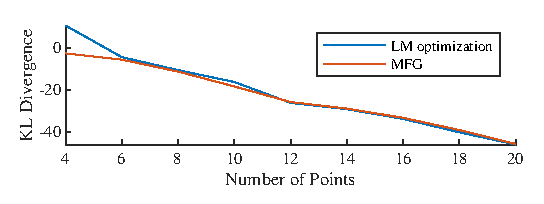
\includegraphics[scale=1.4]{figures/VIO-KL}
	\caption[KL divergence of the MFG and LM-optimization methods.]{KL divergence $d(p||p_\text{MFG})$ and $d(p||p_\text{LM})$ of the MFG and LM-optimization methods.}
	\label{fig:VIO-KL}
\end{figure}

The results are presented in Figure \ref{fig:VIO-KL}.
Because the constant $\log(c)$ is not calculated, the KL divergence in the figure is sometimes negative.
It can be seen that when $N>10$, the KL divergence for the LM method is slightly lower, indicating a slightly better estimation of the uncertainty.
When $N \leq 10$, because the uncertainty in pose increases, the KL-divergence of the MFG becomes smaller.
And when $N=4$, it becomes notably smaller than the LM method, indicating MFG is more accurate when dealing with very large uncertainty in the pose.

Finally, the measurement update algorithm in Table \ref{tab:VIO-update} is combined with the uncertainty propagation in Table \ref{tab:posEst-prop} into a recursive Bayesian filter.
This filter is compared with the MEKF based method in a visual-inertial navigation setting.
A vehicle is supposed to move in a circle with radius of $\SI{3}{\meter}$.
The height of the trajectory is fluctuating between $\SI{0}{\meter}$ and $\SI{1}{\meter}$ as a sinusoidal function with the frequency at $\SI{0.785}{\hertz}$.
The resulting average free acceleration is $\SI{0.51}{\meter/\second\squared}$.
The first body-fixed axis of the vehicle points forward along the tangent direction of the trajectory, and the second body-fixed axis is confined in the horizontal plane, pointing towards the center of the circle.
The resulting average angular velocity is $\SI{24.7}{\deg/\second}$.
A hundred landmarks are scattered around the trajectory in a rectangular shape.
The trajectory of the vehicle and locations of landmarks are depicted in Figure \ref{fig:VIO-trajectory}.
A landmark is measured by the camera only if it is within $\SI{3}{\meter}$ of the vehicle.

\begin{figure}
	\centering
	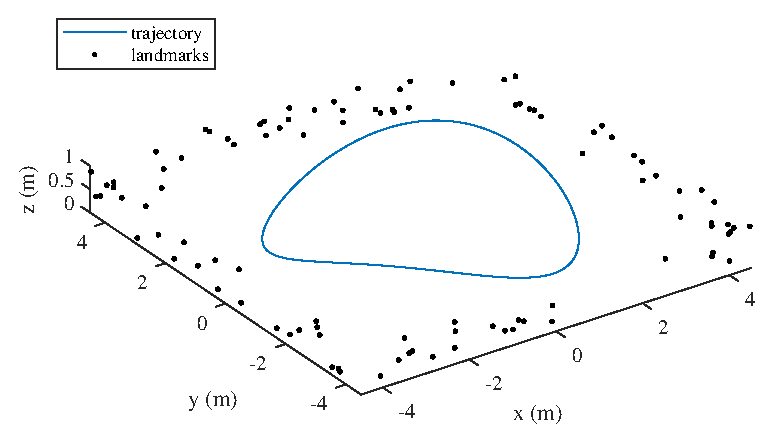
\includegraphics{figures/VIO-trajectory}
	\caption{Trajectory and landmarks for visual-inertial navigation.}
	\label{fig:VIO-trajectory}
\end{figure}

The white noise for the gyroscope is set as $\SI{0.1}{\deg/\sqrt{\second}}$, and for the accelerometer is $\SI{0.1}{\meter/\second/\sqrt{\second}}$.
It is assumed that the gyroscope and accelerometer do not have random walk biases, i.e., $H_{gv}$ in \eqref{eqn:posEst-kinematics-gyrobias} and $H_{av}$ in \eqref{eqn:posEst-kinematics-accebias} are zero, so the biases are not estimated in the filter.
The gyroscope is sampled at $\SI{200}{\hertz}$.
The position measurement noise of the camera is set identically as $\sigma^2I_{3\times 3}$, with $\sigma = \SI{1}{\meter}$.
And the sampling frequency for the camera is at $\SI{10}{\hertz}$.
The simulation lasts for $\SI{40}{\second}$.

Two initial conditions are tested.
For the first case, the initial attitude uncertainty for the MFG filter is $S_0 = 50I_{3\times 3}$, and for MEKF is $0.1^2I_{3\times 3}$.
The initial velocity and position uncertainties for both filters are set as $0.1^2I_{3\times 3}$.
The initial attitude, velocity, and position are their true values plus a random noise sampled from those initial uncertainty distributions.
This corresponds to an initial condition with relatively small uncertainty.
Next, for the second case, the initial conditions for velocity and position are set the same as in the first case.
But the initial attitude is rotated from the true attitude around the inertial vertical axis by $\SI{180}{\deg}$, simulating the scenario when the initial heading direction is completely unknown.
The attitude uncertainty for MFG is set as $S_0 = 0.01I_{3\times 3}$, and for MEKF is $1000I_{3\times 3}$, indicating a very large initial attitude uncertainty.
A hundred Monte Carlo simulations are carried out for both initial conditions, and paired $t$-test is used to find any significant difference with the significant level at $\alpha = 0.001$.

\begin{table}
	\centering
	\footnotesize
	\caption{Estimation error for visual-inertial navigation without map noises}
	\label{tab:VIO-filter-error}
	\begin{tabular}{l|c|c|c|c}
		\hline\hline
		initial condition & \multicolumn{2}{c|}{small uncertainty} & \multicolumn{2}{c}{large uncertainty} \\ \hline
		filter & MFG & MEKF & MFG & MEKF \\ \hline
		att err (deg) & 0.97$\pm$0.21 (p<0.001) & 0.90$\pm$0.20 & 1.62$\pm$0.23 (p<0.001) & 75.0$\pm$38.5 \\
		vel err (m/s) & 0.208$\pm$0.012 (p<0.001) & 0.205$\pm$0.013 & 0.235$\pm$0.013 (p<0.001) & 1.59$\pm$0.54 \\
		pos err (m) & 0.173$\pm$0.011 (p<0.001) & 0.172$\pm$0.011 & 0.184$\pm$0.010 (p<0.001) & 2.37$\pm$1.03 \\
		\hline\hline
	\end{tabular}
\end{table}

\begin{figure}
	\centering
	\includegraphics[scale=1.3]{figures/VIO-filter-error}
	\caption{Error trajectory of a particular simulation for visual-inertial navigation without map noises.}
	\label{fig:VIO-filter-error}
\end{figure}

For the MFG filter, only definition MFGI is tested, because all linear components, i.e., velocity and position, are defined in the inertial frame.
The estimation errors for MFG and MEKF are summarized in Table \ref{tab:VIO-filter-error}.
It demonstrates that MEKF has slightly better accuracy than MFG for the small initial uncertainty case, which is consistent with the results in Table \eqref{tab:VIO-pose-error} for static pose estimation.
But their relative differences are very small compared to the magnitude of error.
On the other hand, for large initial uncertainty, the MFG filter behaves much better than MEKF.
The trajectory of the estimation error for one particular simulation is presented in Figure \ref{fig:VIO-filter-error}.
It is seen that the MEKF suffers from extremely slow convergence from the initially wrong attitude.
Even worse, the wrong attitude estimation for MEKF contributes to the large errors in velocity and position.
This is very similar to the simulation for IMU-GNSS navigation in Figure \ref{fig:posEst-error}.
And the reason for this slow convergence can be attributed to that the Gaussian distribution of MEKF does not properly describe the initial large attitude uncertainty.

\subsection{Pose Estimation With Map Uncertainty} \label{section:VIO-pose-map}

In Chapter \ref{section:VIO-pose}, an algorithm is developed to model the uncertainty of the pose $(R,t)\in\SE{3}$ that aligns two point sets.
In particular, the map point set is assumed to be perfectly known, and the measurement point set is affected by random noises.
However, in some cases the noise of map point set also needs to be modeled.
For example, the 3D coordinates of triangulated features from a stereo camera have larger noises when the feature is further away from the camera, so it may be beneficial to also model the uncertainty of those triangulated map points.
In this subsection, the MFG is used to model the pose where the map point set also suffers from noises.

Suppose there are $N$ landmarks, whose coordinates in the inertial frame are denoted by $\{p_i\}_{i=1}^N$.
The coordinates are randomly distributed by $p_i \sim \mathcal{N}(\bar{p}_i, B_i)$.
These map points are measured by a camera in the body fixed frame as $\{p'_i\}_{i=1}^N$, affected by Gaussian noises with zero mean and covariance matrices $A_i = \sigma_i^2I_{3\times 3}$.
Note that only the noise of measurements $A_i$ is assumed to be isotropic.
If there is no prior information for the pose (non-informative prior), the posterior density function for the pose and map, according to the Bayes' formula, is given by
\begin{align} \label{eqn:VIO-likelihood-map}
	p\left( R,t,\{p_i\} | \{p'_i\} \right) &\propto \expb{-\tfrac{1}{2} \sum_{i=1}^{N} \big(R^T(p_i-t)-p'_i\big)^T A_i^{-1} \big(R^T(p_i-t)-p'_i\big)} \nonumber \\
	&\qquad\qquad \cdot \expb{-\tfrac{1}{2}\sum_{i=1}^N (p_i-\bar{p}_i)^T B_i^{-1} (p_i-\bar{p}_i)}.
\end{align}
The first exponential term in the above equation is the likelihood \eqref{eqn:VIO-likelihood} considered in Chapter \ref{section:VIO-pose}, and the last term is the prior density function for map points.
The objective is to model the pose $(R,t)|\{p'_i\}$ with an MFG, and to find the posterior Gaussian distribution for each map point $p_i|\{p'_i\}$.

Because the coordinates of map points $p_i$ are now random variables, the algorithm developed in Chapter \ref{section:VIO-pose} cannot be directly used.
But in the next lemma, it is shown that \eqref{eqn:VIO-likelihood-map} can be decomposed into two parts, and one of them has exactly the same structure as \eqref{eqn:VIO-likelihood}, so the algorithm in Chapter \ref{section:VIO-pose} can be applied.

\begin{lemma} \label{lemma:VIO-likelihood-map-factor}
	Let $\delta p_i = p_i-\bar{p}_i \in \mathbb{R}^3$ for $i=1,\dots,N$. Equation \eqref{eqn:VIO-likelihood-map} can be decomposed into
	\begin{align}
		p(R,t,\{p_i\}|\{p'_i\}) = p(R,t|\{p'_i\}) p(\{\delta p_i\}|R,t,\{p'_i\}),
	\end{align}
	where $p(R,t|\{p'_i\})$ is
	\begin{align} \label{eqn:VIO-likelihood-map-Rt}
		\expb{-\tfrac{1}{2} \sum_{i=1}^N \big(R^T(\bar{p}_i-t)-p'_i\big)^T (A_i+R^TB_iR)^{-1} \big(R^T(\bar{p}_i-t)-p'_i\big)}.
	\end{align}
	Let $K_i = (A_i^{-1}+B_i^{-1})^{-1} A_i^{-1} \in \mathbb{R}^{3\times 3}$, then $p(\{\delta p_i\}|R,t,\{p'_i\})$ is
	\begin{align} \label{eqn:VIO-likelihood-map-p}
		\expb{-\tfrac{1}{2} \sum_{i=1}^N \left( \delta p_i - K_i(Rp'_i+t-\bar{p}_i) \right)^T (A_i^{-1}+B_i^{-1}) \left( \delta p_i - K_i(Rp'_i+t-\bar{p}_i) \right)}.
	\end{align}
\end{lemma}
\begin{proof}
	Because $A_i = \sigma_i^2I_{3\times 3}$, for $R\in\SO{3}$, $RA_i^{-1}R^T = A_i^{-1}$.
	For $i=1,\ldots,N$, the exponent of \eqref{eqn:VIO-likelihood-map} can be written as
	\begin{align*}
		&\big(R^T(p_i-t)-p'_i\big)^T A_i^{-1} \big(R^T(p_i-t)-p'_i\big) + (p_i-\bar{p}_i)^T B_i^{-1} (p_i-\bar{p}_i) \\
		= &(\bar{p}_i+\delta p_i - t - Rp'_i)^T A_i^{-1} (\bar{p}_i+\delta p_i - t - Rp'_i) + \delta p_i^T B_i^{-1} \delta p_i \\
		= &(Rp'_i+t-\bar{p}_i)^T A_i^{-1} (Rp'_i+t-\bar{p}_i) - 2\delta p_i^T A_i^{-1} (Rp'_i+t-\bar{p}_i) + \delta p_i^T (A_i^{-1}+B_i^{-1}) \delta p_i.
	\end{align*}
	The last two terms can be further arranged into a quadratic form as
	\begin{align*}
		&\delta p_i^T (A_i^{-1}+B_i^{-1}) \delta p_i - 2\delta p_i^T A_i^{-1} (Rp'_i+t-\bar{p}_i) \\
		= &\left( \delta p_i - K_i(Rp'_i+t-\bar{p}_i) \right)^T (A_i^{-1}+B_i^{-1}) \left( \delta p_i - K_i(Rp'_i+t-\bar{p}_i) \right) \\
		&\qquad - (Rp'_i+t-\bar{p}_i)^T A_i^{-1} (A_i^{-1}+B_i^{-1})^{-1} A_i^{-1} (Rp'_i+t-\bar{p}_i).
	\end{align*}
	Using Woodbury matrix identity \cite{petersen2008matrix}, $(Rp'_i+t-\bar{p}_i)^T A_i^{-1} (Rp'_i+t-\bar{p}_i)$ and the last term in the above equation can be combined into
	\begin{align*}
		&(Rp'_i+t-\bar{p}_i)^T A_i^{-1} (Rp'_i+t-\bar{p}_i) - (Rp'_i+t-\bar{p}_i)^T A_i^{-1} (A_i^{-1}+B_i^{-1})^{-1} A_i^{-1} (Rp'_i+t-\bar{p}_i) \\
		&\qquad = (Rp'_i+t-\bar{p}_i)^T \Big[ A_i^{-1} - A_i^{-1} (A_i^{-1}+B_i^{-1})^{-1} A_i^{-1} \Big] (Rp'_i+t-\bar{p}_i) \\
		&\qquad = (Rp'_i+t-\bar{p}_i)^T (A_i+B_i)^{-1} (Rp'_i+t-\bar{p}_i) \\
		&\qquad = \big(R^T(\bar{p}_i-t)-p'_i\big)^T (A_i+R^TB_iR)^{-1} \big(R^T(\bar{p}_i-t)-p'_i\big).
	\end{align*}
	And the desired decomposition is derived.
\end{proof}

The density $p(R,t|\{p'_i\})$ in \eqref{eqn:VIO-likelihood-map-Rt} has exactly the same structure as \eqref{eqn:VIO-likelihood}, except the noise is increased from $A_i$ to $A_i+R^TB_iR$.
So using Theorem \ref{thm:VIO-factor} and \eqref{eqn:VIO-likelihood-marginal-q}, $p(R,t|\{p'_i\})$ can be further decomposed into
\begin{align} \label{eqn:VIO-likelihood-map-Rt-factor}
	&p(R,t|\{p'_i\}) = \expb{-\tfrac{1}{2} (\bm{q}'-\bm{q}_m)^T \big(\mathbf{T}\mathbf{A}\mathbf{T}^T\big)^{-1} (\bm{q}'-\bm{q}_m)} \nonumber \\
	&\qquad \cdot \expb{-\tfrac{1}{2} (t - \mu_{t|R})^T (RCR^T)^{-1} (t - \mu_{t|R})} \triangleq p(R|\{p'_i\}) p(t|R,\{p'_i\}),
\end{align}
where $\bm{q}'$ and $\bm{q}_m$ are defined in \eqref{eqn:VIO-centering}, with $p_i$ replaced by $\bar{p}_i$.
The covariance matrix $\mathbf{A} = \diag(A_1+RB_1R^T, \ldots, A_N+RB_NR^T)$, and $\mathbf{T}$, $\mu_{t|R}$ are defined in Theorem \ref{thm:VIO-factor}.
The first exponential term $p(R|\{p'_i\})$ can be matched to a matrix Fisher density using the algorithm in Table \ref{tab:VIO-marginal}, with $A_i$ replaced by $A_i+B_i$.
Note that although the definition of $\mathbf{A}$ has $RB_iR^T$, it can be simply replaced by $B_i$ in the proposal distribution for importance sampling, as the proposal distribution only needs to be close to the target distribution.

Let the approximated parameter of the matrix Fisher distribution be denoted by $F$.
And let $F = USV^T$ be its pSVD, define $\nu_R = (QS-SQ^T)^\vee$ for MFGI, or $\nu_R = (SQ-Q^TS)^\vee$ for MFGB, with $Q = U^TRV$ as before.
The next step is to study the density function
\begin{align*}
	p(t|R,\{p'_i\}) p(\{\delta p_i\}|R,t,\{p'_i\})
\end{align*}
conditioned by $R$.
The next lemma deals with this density.

\begin{lemma} \label{lemma:VIO-likelihood-tp}
	Let $\bm{x} = \left[p_1^T, \cdots, p_N^T, t^T\right]^T \in \mathbb{R}^{3N+3}$, and $\bm{\mu}_{x|R} = \left[\mu_{p_1|R}^T, \cdots, \mu_{p_N|R}^T, \mu_{t|R}^T\right]^T \in \mathbb{R}^{3N+3}$, where $\mu_{p_i|R} = (I_{3\times 3}-K_i)\bar{p}_i + K_i(Rp'_i+\mu_{t|R})$.
	Also, let $\bm{\Sigma}_{x|R}$ be defined as
	\begin{align} \label{eqn:VIO-likelihood-map-Sigmax}
		\bm{\Sigma}_{x|R} = \begin{bmatrix}
			A_1^{-1}+B_1^{-1} & \cdots & 0_{3\times 3} & -A_1^{-1} \\
			\vdots & \ddots & \vdots & \vdots \\
			0_{3\times 3} & \cdots & A_N^{-1}+B_N^{-1} & -A_N^{-1} \\
			-A_1^{-1} & \cdots & -A_N^{-1} & (RCR^T)^{-1} + \sum_{i=1}^N A_i^{-1}\left( A_i^{-1}+B_i^{-1} \right)^{-1} A_i^{-1}
		\end{bmatrix}^{-1}.
	\end{align}
	Then the conditional density can be written as
	\begin{align} \label{eqn:VIO-likelihood-map-tp}
		p(t|R,\{p'_i\}) p(\{\delta p_i\}|R,t,\{p'_i\}) = \expb{-\tfrac{1}{2} (\bm{x}-\bm{\mu}_{x|R})^T \bm{\Sigma}_{x|R}^{-1} (\bm{x}-\bm{\mu}_{x|R})}.
	\end{align}
\end{lemma}
\begin{proof}
	The mean of $\delta p_i$ in \eqref{eqn:VIO-likelihood-map-p} can be arranged into
	\begin{align*}
		K_i(Rp'_i+t-\bar{p}_i) = K_i(Rp'_i+\mu_{t|R}-\bar{p}_i) + K_i(t-\mu_{t|R}).
	\end{align*}
	Let $\mu_{\delta p_i|R} = K_i(Rp'_i+\mu_{t|R}-\bar{p}_i)$, then the exponent of $p(\{\delta p_i\}|R,t,\{p'_i\})$ becomes
	\begin{align*}
		&\left( \delta p_i - K_i(Rp'_i+t-\bar{p}_i) \right)^T (A_i^{-1}+B_i^{-1}) \left( \delta p_i - K_i(Rp'_i+t-\bar{p}_i) \right) \\
		= &\left( \begin{bmatrix} I_{3\times 3} & -K_i \end{bmatrix} \begin{bmatrix} \delta p_i - \mu_{\delta p_i|R} \\ t-\mu_{t|R} \end{bmatrix} \right)^T (A_i^{-1} + B_i^{-1}) \left( \begin{bmatrix} I_{3\times 3} & -K_i \end{bmatrix} \begin{bmatrix} \delta p_i - \mu_{\delta p_i|R} \\ t-\mu_{t|R} \end{bmatrix} \right) \\
		= &\begin{bmatrix} p_i - \mu_{p_i|R} \\ t-\mu_{t|R} \end{bmatrix}^T \begin{bmatrix} A_i^{-1} + B_i^{-1} & -A_i^{-1} \\ -A_i^{-1} & A_i^{-1}(A_i^{-1} + B_i^{-1})A_i^{-1} \end{bmatrix} \begin{bmatrix} p_i - \mu_{p_i|R} \\ t-\mu_{t|R} \end{bmatrix}.
	\end{align*}
	And \eqref{eqn:VIO-likelihood-map-tp} can be proved by summing up the above equations for $i=1,\ldots,N$, and $(t-\mu_{t|R})^T(RCR^T)^{-1}(t-\mu_{t|R})$.
\end{proof}

The conditional density for the map coordinates $\{p_i\}$ and translation $t$ is written into a Gaussian density in \eqref{eqn:VIO-likelihood-map-tp}, with the mean and variance dependent on $R$.
Because the objective is to match an MFG to $(R,t)|\{p'_i\}$, and Gaussian distributions to $p_i|\{p'_i\}$, only the covariance matrices for $t$ and each of $p_i$ are needed.
Namely, the diagonal blocks of $\Sigma_{x|R}$ in \eqref{eqn:VIO-likelihood-map-Sigmax} need to be evaluated, whereas the off-diagonal blocks representing correlations are neglected.
Using the block inversion formula, the $i$-th 3-by-3 diagonal block of $\bm{\Sigma}_{x|R}$ representing the conditional covariance matrix for $p_i$ is
\begin{align}
	\Sigma_{p_i|R} = B_i - B_i \left[ (A_i+B_i)^{-1} (A_i+B_i - RCR^T) (A_i+B_i)^{-1} \right] B_i.
\end{align}
And the last 3-by-3 diagonal block of $\bm{\Sigma}_{x|R}$ representing the conditional covariance matrix for $t$ is
\begin{align}
	\Sigma_{t|R} = RCR^T.
\end{align}
In other words, when matching $(R,t)|\{p'_i\}$ to an MFG, the map coordinates $\{p_i\}$ are marginalized; and when matching $p_i|\{p'_i\}$ to a Gaussian distribution, the pose $(R,t)$ and all other $\{p_j\}$ with $i\neq j$ are marginalized.

Before giving necessary moments for the conditional MLE of $t|R$, and the first two moments for $p_i$, note that the expressions of $C$ and $\mathbf{D}$ in \eqref{eqn:VIO-likelihood-C} and $\eqref{eqn:VIO-likelihood-D}$ are now defined using $\mathbf{A} = \diag(A_1+RB_1R^T, \ldots, A_N+RB_NR^T)$ in \eqref{eqn:VIO-likelihood-map-Rt} in this subsection.
So a similar lemma as Lemma \ref{lemma:VIO-likelihood-CD} is needed to simplify calculations.

\begin{lemma}
	Define $\tilde{C} = RCR^T \in \mathbb{R}^{3\times 3}$, and $\tilde{\mathbf{D}} \in \mathbb{R}^{3\times 3N}$ such that the $i$-th 3-by-3 column block of $\tilde{\mathbf{D}}$ is $\tilde{D}_i = RD_iR^T$.
	If the expressions of $C$ and $\mathbf{D}$ in \eqref{eqn:VIO-likelihood-C} and $\eqref{eqn:VIO-likelihood-D}$ are defined using $\mathbf{A} = \diag(A_1+RB_1R^T, \ldots, A_N+RB_NR^T)$, then $\tilde{C}$ and $\tilde{\mathbf{D}}$ have the same expressions as $C$ and $\mathbf{D}$ with $\mathbf{A} = \diag(A_1+B_1,\ldots,A_N+B_N)$.
\end{lemma}
\begin{proof}
	This lemma is a straightforward extension of Lemma \ref{lemma:VIO-likelihood-CD}.
\end{proof}

With the above lemma, the expressions for $\tilde{C}$ and $\tilde{\mathbf{D}}$ do not dependent on $R$ anymore.
Also, the conditional mean $\mu_{t|R}$ is simplified as follows
\begin{align}
	\mu_{t|R} = \sum_{i=1}^N \tilde{D}_i(Rp'_i-\bar{p}_i).
\end{align}
With these simplifications, the conditional mean $\mu_{t|R}$ and covariance matrices $\Sigma_{x|R}$ has exactly the same expression as in \eqref{eqn:VIO-likelihood-conditional-sim}, so the moments $\expect{t}$, $\expect{t\nu_R^T}$, and $\expect{tt^T}$ according to \eqref{eqn:VIO-likelihood-map-tp}, that are necessary for the conditional MLE, can be calculated as in Theorem \ref{thm:VIO-conditional} or Theorem \ref{thm:VIO-conditional-sim}, with $C$, $D_i$, and $p_i$ replaced by $\tilde{C}$, $\tilde{D}_i$, and $\bar{p}_i$, depending on whether $A_1+B_1 = \cdots = A_N+B_N$.
Also, the moments $\expect{p_i}$ and $\expect{p_ip_i^T}$ are given as follows.

\begin{theorem} \label{thm:VIO-likelihood-Ep}
	The moments $\expect{p_i}$ and $\expect{p_ip_i^T}$ according to \eqref{eqn:VIO-likelihood-map-tp} can be calculated as
	\begin{align}
		\expect{p_i} &= (I_{3\times 3}-K_i)\bar{p}_i + K_i(\expect{R}p'_i+\expect{\mu_{t|R}}) \\
		\expect{p_ip_i^T} &= \Sigma_{p_i|R} + (I_{3\times 3}-K_i)\bar{p}_i\bar{p}_i^T(I_{3\times 3}-K_i)^T + (I_{3\times 3}-K_i)\bar{p}_i (\expect{R}p'_i+\expect{\mu_{t|R}})^TK_i^T \nonumber \\
		&\quad + K_i \left(\expect{Rp'_i(p'_i)^TR^T} + \expect{Rp'_i\mu_{t|R}^T} + \expect{\mu_{t|R}(p'_i)^TR^T} + \expect{\mu_{t|R}\mu_{t|R}^T}\right) K_i^T \nonumber \\
		&\quad + K_i(\expect{R}p'_i+\expect{\mu_{t|R}})\bar{p}_i^T(I_{3\times 3}-K_i)^T,
	\end{align}
	where $\expect{\mu_{t|R}} = \expect{t}$, $\expect{\mu_{t|R}\mu_{t|R}^T} = \expect{tt^T} - \tilde{C}$.
	Also, if $A_1+B_1 = \cdots = A_N+B_N$, then
	\begin{align}
		\expect{\mu_{t|R}(p'_i)^TR^T} = \bar{p}_c(p'_i)^T\expect{R}^T - \expect{Rp'_c(p'_i)^TR^T},
	\end{align}
	otherwise
	\begin{align}
		\expect{\mu_{t|R}(p'_i)^TR^T} = \sum_{j=1}^N \tilde{D}_j \left(\expect{Rp'_j(p'_i)^TR^T} - \bar{p}_j(p'_i)^T\expect{R}^T\right).
	\end{align}
\end{theorem}
\begin{proof}
	These moments can be calculated by integrating the left hand side with respect to the conditional density \eqref{eqn:VIO-likelihood-map-tp}, and noting that the marginal distribution of a multi-variate Gaussian distribution is also Gaussian with the corresponding mean and covariance matrix.
	Then the results are further integrated with respect to the marginal distribution for $R$, which has already been matched to a matrix Fisher distribution with parameter $F$.
\end{proof}

With the moments $\expect{p_i}$ and $\expect{p_ip_i^T}$, the distribution for $p_i$ can be matched to a Gaussian distribution with the same first and second order moments.
In summary, the posterior density \eqref{eqn:VIO-likelihood-map} has been approximated by an MFG for the pose $(R,t)$, and $N$ Gaussian distributions for the map coordinates $\{p_i\}_{i=1}^N$.
The pseudocode is summarized in Table \ref{tab:VIO-pose-map}.

\begin{table}
	\caption{Pose and map coordinates estimation with map noises}
	\label{tab:VIO-pose-map}
	\begin{algorithmic}[1]
		\algrule[0.8pt]
		\Procedure{($\mathcal{MG}, \{\mathcal{N}_i^+\}) = $ Pose-Map Estimation}{$\{p'_i\}$, $\{\mathcal{N}_i(\bar{p}_i,B_i)\}$}
		\algrule
		\State Obtain $F=$ Attitude Estimation($\{\bar{p}_i\}$, $\{p'_i\}$) in Table \ref{tab:VIO-marginal} with $A_i$ replaced by $A_i+B_i$, and $\expb{-\tfrac{1}{2}f_R(R)}$ as the first term on the right hand side of \eqref{eqn:VIO-likelihood-map-Rt-factor}.
		\State Let $F = USV^T$ be its pSVD.
		\State Calculate $\expect{\nu_R\nu_R^T}$ as in \eqref{eqn:MFG-EvRvR} using $S$.
		\If{$A_1+B_1 = \cdots = A_N+B_N$}
		\State Calculate $\expect{t}$, $\expect{t\nu_R^T}$, and $\expect{tt^T}$ in Theorem \ref{thm:VIO-conditional-sim}, with $\tfrac{\sigma^2}{N}I_{3\times 3}$ replaced by $\tfrac{A+B}{N}$, and $p_i$ replaced by $\bar{p}_i$.
		\Else
		\State Calculate $\expect{t}$, $\expect{t\nu_R^T}$, and $\expect{tt^T}$ in Theorem \ref{thm:VIO-conditional}, with $C$, $D_i$, and $p_i$ replaced by $\tilde{C}$, $\tilde{D}_i$, and $\bar{p}_i$.
		\EndIf
		\State Obtain $\mu$, $\Sigma$, $P$ according to Theorem \ref{thm:MFG-MLE-conditional}, with $\expect{t}$, $\expect{t\nu_R^T}$, $\expect{tt^T}$, $\expect{\nu_R\nu_R^T}$, and $\expect{\nu_R} = 0$.
		\State Set $\mathcal{MG} = \mathcal{MG}(\mu,\Sigma,P,U,S,V)$.
		\State For $i=1,\ldots,N$, calculate $\expect{p_i}$ and $\expect{p_ip_i^T}$ in Theorem \ref{thm:VIO-likelihood-Ep}.
		\State Set $\mathcal{N}_i^+$ as $\mathcal{N}(\expect{p_i}, \expect{p_ip_i^T}-\expect{p_i}\expect{p_i}^T)$.
		\EndProcedure
		\algrule[0.8pt]
	\end{algorithmic}
\end{table}

Next, then case when there is a prior density for the pose $(R,t)$ is also considered, so that the algorithm can be applied in a recursive filter.
Similar to Chapter \ref{section:VIO-pose}, let $y = [t^T, a^T]^T \in \mathbb{R}^n$, suppose $(R,y)$ follows an MFG with the parameter $(\mu,\Sigma,P,U,S,V)$ before measurements, where $a$ includes other Euclidean quantities, such as linear velocity and sensor biases.
According to the Bayes' formula, the posterior density for the pose $(R,y)$ and map coordinates $\{p_i\}$ after incorporating the measurements $\{p'_i\}$ is
\begin{align} \label{eqn:VIO-map-posterior}
	&p(R,y,\{p_i\}|\{p'_i\}) = \expb{-\tfrac{1}{2}\sum_{i=1}^N \big(R^T(p_i-Hy)-p'_i\big)^T A_i^{-1} \big(R^T(p_i-Hy)-p'_i\big)} \nonumber \\
	&\qquad \cdot \expb{-\tfrac{1}{2}\sum_{i=1}^N (p_i-\bar{p}_i)^T B_i^{-1} (p_i-\bar{p}_i)} \cdot \etr{FR^T} \expb{-\tfrac{1}{2}(y-\mu_c)^T \Sigma_c^{-1} (y-\mu_c)},
\end{align}
where $F$, $\mu_c$, $\Sigma_c$ are defined with respect to $\mathcal{MG}(\mu,\Sigma,P,U,S,V)$.
According to Lemma \ref{lemma:VIO-likelihood-map-factor}, Lemma \ref{lemma:VIO-likelihood-tp}, and \eqref{eqn:VIO-likelihood-map-Rt-factor}, the above density can be decomposed into
\begin{align} \label{eqn:VIO-map-posterior-factor1}
	&p(R,y,\{p_i\}|\{p'_i\}) = \etr{FR^T} \expb{-\tfrac{1}{2} (\bm{q}'-\bm{q}_m)^T \big(\mathbf{T}\mathbf{A}\mathbf{T}^T\big)^{-1} (\bm{q}'-\bm{q}_m)} \nonumber \\
	&\qquad \cdot \expb{-\tfrac{1}{2} (\bm{x}-\bm{\mu}_{x|R})^T \bm{\Sigma}_{x|R}^{-1} (\bm{x}-\bm{\mu}_{x|R})} \expb{-\tfrac{1}{2}(y-\mu_c)^T \Sigma_c^{-1} (y-\mu_c)}.
\end{align}
As before, this density function is factorized into a marginal density for $R$, and a conditional density for $t|R$, and $\{p_i\}|R$.

\begin{theorem} \label{thm:VIO-map-posterior}
	Let $z = [\bm{x}^T, a^T]^T \in \mathbb{R}^{3N+n}$, $H = \big[ I_{(3N+3)\times (3N+3)}, 0_{(3N+3)\times (n-3)} \big]$, and $G = \big[ 0_{n\times 3N}, I_{n\times n} \big]$.
	Define $\mu_{z|R}$ as
	\begin{align}
		\mu_{z|R} = \left( H^T\bm{\Sigma}_{x|R}^{-1}H + G^T\Sigma_c^{-1}G \right)^{-1} \left( H^T\bm{\Sigma}_{x|R}^{-1}\bm{\mu}_{x|R} + G^T\Sigma_c^{-1}\mu_c \right),
	\end{align}
	and $\Sigma_{z|R}$ as
	\begin{align}
		\Sigma_{z|R} = \left( H^T\bm{\Sigma}_{x|R}^{-1}H + G^T\Sigma_c^{-1}G \right)^{-1}.
	\end{align}
	Also, let $\mu_{c,t}$ and $\Sigma_{c,t}$ be the appropriate blocks in $\mu_c$ and $\Sigma_c$ for $t$.
	Then the posterior density $p(R,y,\{p_i\}|\{p'_i\})$ can be written as
	\begin{align} \label{eqn:VIO-map-posterior-factor2}
		&p(R,y,\{p_i\}|\{p'_i\}) = \etr{FR^T} \expb{-\tfrac{1}{2} (\bm{q}'-\bm{q}_m)^T \big(\mathbf{T}\mathbf{A}\mathbf{T}^T\big)^{-1} (\bm{q}'-\bm{q}_m)} \nonumber \\
		&\ \cdot \expb{-\tfrac{1}{2}(\mu_{t|R}-\mu_{c,t})^T (\Sigma_{t|R} + \Sigma_{c,t})^{-1} (\mu_{t|R}-\mu_{c,t})} \expb{-\tfrac{1}{2}(z-\mu_{z|R})^T \Sigma_{z|R}^{-1} (z-\mu_{z|R})}.
	\end{align}
\end{theorem}
\begin{proof}
	The proof is given in Appendix \ref{app:VIO-map-posterior}.
\end{proof}

The key point is that the first three terms on the right hand side of \eqref{eqn:VIO-map-posterior-factor2} do not depend on $z$, so they can be matched to a matrix Fisher distribution using the progressive update method in Table \ref{tab:posEst-update-att}.
As before, let the approximated parameter of the matrix Fisher distribution be denoted by $F^+$.
And let $F^+ = U^+S^+(V^+)^T$ be its pSVD, define $\nu_R = (Q^+S^+-S^+(Q^+)^T)^\vee$ for MFGI, or $\nu_R = (S^+Q^+-(Q^+)^TS^+)^\vee$ for MFGB, with $Q^+ = (U^+)^TR^+V^+$.
Similar to the case without pose prior, the next step is to calculate the moments for $y|R$ with $\{p_i\}$ marginalized out; and the moments for $p_i$, with $(R,y)$ and other $\{p_j\}$, $i\neq j$, marginalized out.
These moments are according to the posterior density \eqref{eqn:VIO-map-posterior-factor2}, and to distinguish with those according to the prior distribution $\mathcal{MG}(\mu,\Sigma,P,U,S,V)$, they are denoted by $\expect{\cdot | \mathcal{Z}}$, where $\mathcal{Z} = \{p'_i\}_{i=1}^N$ are all measurements.
The calculations for these moments are relegated to Theorem \ref{thm:VIO-map-posterior-moments} in Appendix \ref{app:VIO-map-posterior}.

Using the moments $\expect{y|\mathcal{Z}}$, $\expect{y(\nu_R^+)^T|\mathcal{Z}}$, and $\expect{yy^T|\mathcal{Z}}$, the posterior density for $(R,t)$ is matched to an MFG using the conditional MLE in Theorem \ref{thm:MFG-MLE-conditional}.
And using the moments $\expect{p_i|\mathcal{Z}}$ and $\expect{p_ip_i^T|\mathcal{Z}}$, the posterior density for $p_i$ is matched to a Gaussian distribution, for $i=1,\ldots,N$.
The pseudocode is summarized in Table \ref{tab:VIO-map-update}.

\begin{table}
	\caption{Measurement update with map noises}
	\label{tab:VIO-map-update}
	\begin{algorithmic}[1]
		\algrule[0.8pt]
		\Procedure{$(\mathcal{MG}^+,\{\mathcal{N}_i^+\})$ = Measurement Update}{$\mathcal{MG}^-$, $\{\mathcal{N}_i^-(\bar{p}_i,B_i)\}$, $\{p'_i\}$}
		\algrule
		\State Let $F^- = U^-S^-(V^-)^T$.
		\State Calculate $F^+=$ Attitude Update($F^-$, $\{\bar{p}_i\}$, $\{p'_i\}$) in Table \ref{tab:VIO-update}, where $f_m(R)$ is the second and third term on the right hand side of \eqref{eqn:VIO-map-posterior-factor2}.
		\State Let the pSVD of $F^+$ be $F^+ = U^+S^+(V^+)^T$.
		\State Calculate $\expect{y|\mathcal{Z}}$, $\expect{y(\nu_R^+)^T|\mathcal{Z}}$, and $\expect{yy^T|\mathcal{Z}}$ in Theorem \ref{thm:VIO-map-posterior-moments}.
		\State Obtain $\mu^+$, $\Sigma^+$, and $P^+$ using the conditional MLE in Theorem \ref{thm:MFG-MLE-conditional}.
		\State Set $\mathcal{MG}^+ = \mathcal{MG}(\mu^+,\Sigma^+,P^+,U^+,S^+,V^+)$.
		\State For $i=1,\ldots,N$, calculate $\expect{p_i|\mathcal{Z}}$ and $\expect{p_ip_i^T|\mathcal{Z}}$ in Theorem \ref{thm:VIO-map-posterior-moments}.
		\State Set $\mathcal{N}_i^+$ as $\mathcal{N}(\expect{p_i|\mathcal{Z}}, \expect{p_ip_i^T|\mathcal{Z}}-\expect{p_i|\mathcal{Z}}\expect{p_i|\mathcal{Z}}^T)$.
		\EndProcedure
		\algrule[0.8pt]
	\end{algorithmic}
\end{table}

\subsection{Numerical Simulations With Map Uncertainty}

The proposed method in the previous subsection that uses an MFG to model the pose that aligns two points set with noises is compared with an LM optimization method in this subsection.

First, the estimation algorithm in Table \ref{tab:VIO-pose-map} without pose prior is tested.
The true attitude is set as $R_t = \expb{\tfrac{\pi}{2}\hat{e}_3}$, and the true translation is $t_t = [5,0,0]^T$.
There are 10 map points, scattered as $\bar{p}_i = t_t + \xi_i$, where $\xi_i\in\mathbb{R}^3$ is a three dimensional uniform distribution on $[0,1]^3$.
The prior noise of $p_i$ are grouped into two levels, $N_1$ of them have small noise as $B_i = 0.1^2I_{3\times}$, and $10-N_1$ of them have large noise as $B_i = 1^2I_{3\times 3}$.
The measurement noise is set as $A_i = 0.1^2I_{3\times 3}$ for all $i=1,\ldots,10$.
The number $N_1$ is varied in $\{0,2,4,6,8,10\}$.
For each $N_1$, a thousand Monte Carlo simulations are carried out.
Paired $t$-tests are used to compare the attitude, translation, and map coordinate errors of the MFG algorithm and LM optimization.

\begin{table}
	\centering
	\caption{Pose and map coordinates errors with map uncertainty}
	\label{tab:VIO-error-pose-map}
	\footnotesize
	\begin{tabular}{l|ccc}
		\hline\hline
		estimator & \multicolumn{3}{c}{MFG} \\ \hline
		$N_1$ & 10 & 8 & 6 \\ \hline
		att err (deg) & 9.98$\pm$4.21 (p=0.061) & 10.7$\pm$4.9 (p=0.213) & 13.4$\pm$5.9 (p<0.001) \\
		pos err & 0.173$\pm$0.082 (p=0.240) & 0.198$\pm$0.098 (p=0.048) & 0.237$\pm$0.112 (p<0.001) \\
		map err ($N_1$) & 0.1237$\pm$0.0165 (p<0.001) & 0.126$\pm$0.020 (p<0.001) & 0.130$\pm$0.024 (p<0.001) \\
		map err ($10-N_1$) & - & 0.187$\pm$0.057 (p<0.001) & 0.205$\pm$0.050 (p<0.001) \\
		\midrule[1.2pt]
		estimator & \multicolumn{3}{c}{LM optimization} \\ \hline
		$N_1$ & 10 & 8 & 6 \\ \hline
		att err (deg) & 9.96$\pm$4.20 & 10.7$\pm$4.9 & 13.0$\pm$5.8 \\
		pos err & 0.174$\pm$0.083 & 0.197$\pm$0.099 & 0.230$\pm$0.113 \\
		map err ($N_1$) & 0.1241$\pm$0.0165 & 0.127$\pm$0.020 & 0.131$\pm$0.024 \\
		map err ($10-N_1$) & - & 0.191$\pm$0.058 & 0.209$\pm$0.050 \\
		\hline\hline
		estimator & \multicolumn{3}{c}{MFG} \\ \hline
		$N_1$ & 4 & 2 & 0 \\ \hline
		att err (deg) & 16.5$\pm$7.9 (p<0.001) & 50.6$\pm$30.9 (p<0.001) & 77.1$\pm$41.1 (p=0.056) \\
		pos err & 0.305$\pm$0.147 (p<0.001) & 0.755$\pm$0.372 (p=0.005) & 1.05$\pm$0.38 (p<0.001) \\
		map err ($N_1$) & 0.138$\pm$0.030 (p=0.033) & 0.149$\pm$0.046 (p<0.001) & - \\
		map err ($10-N_1$) & 0.225$\pm$0.056 (p<0.001) & 0.501$\pm$0.189 (p<0.001) & 0.661$\pm$0.173 (p<0.001) \\
		\midrule[1.2pt]
		estimator & \multicolumn{3}{c}{LM optimization} \\ \hline
		$N_1$ & 4 & 2 & 0 \\ \hline
		att err (deg) & 16.0$\pm$7.5 & 48.6$\pm$29.5 & 76.4$\pm$40.8 \\
		pos err & 0.294$\pm$0.149 & 0.772$\pm$0.455 & 1.17$\pm$0.55 \\
		map err ($N_1$) & 0.138$\pm$0.030 & 0.153$\pm$0.048 & - \\
		map err ($10-N_1$) & 0.230$\pm$0.056 & 0.518$\pm$0.216 & 0.708$\pm$0.196 \\
		\hline\hline
	\end{tabular}
\end{table}

The estimation errors are summarized in Table \ref{tab:VIO-error-pose-map}.
Generally speaking, the MFG algorithm has slightly worse accuracy in pose estimation, especially when $N_1 = 4$ and 6, indicating it may have degraded performance when the map prior has mixed uncertainty levels.
But when $N_1 = 0$, the translation error for MFG is significantly smaller than LM optimization, which is consistent with the results in Table \ref{tab:VIO-pose-error}.
Namely, when the pose has large uncertainty, the MFG is better at estimating the translation.
Next, looking at the map coordinate errors, in general the MFG algorithm is more accurate, especially for those points with large prior noises, where the differences are significant for all cases.
The reason for this better performance of MFG is to be investigated in future works, but a guess is that the gradient based optimization may not be very effective for high dimensional variable space, which is 66 in this simulation study; or that the parameters for the LM method is not properly tuned for this high dimensional space.

Next, the measurement update algorithm in Table \ref{tab:VIO-map-update} is combined with the uncertainty propagation for IMU in Table \ref{tab:posEst-prop} into a Bayesian filter for visual-inertial navigation.
And this filter is compared with an MEKF based SLAM algorithm which also estimates the map point coordinates.
In this simulation study, a vehicle is supposed to follow the same trajectory and rotational motion introduced in the simulation in Chapter \ref{section:VIO-simulation}.
The distribution of landmarks, noise parameters for the IMU, sampling frequencies for the IMU and camera are also chosen to be the same.
There are in total 400 landmarks, and the measurement noise of the camera is set as $A_i = 0.05^2I_{3\times 3}$.
Only the landmarks that are within $\SI{3}{\meter}$ from the vehicle are measured by the camera.
The simulation lasts for forty seconds.

Three cases are tested.
The first case is a \textit{normal} condition: the prior noise for all map coordinates are $B_i = 0.1^2I_{3\times 3}$.
The initial attitude, velocity, and position uncertainty for MEKF is set as $0.1^2I_{3\times 3}$; and the initial attitude uncertainty for MFG is $S_0 = 50I_{3\times 3}$.
The initial attitude, velocity, and position estimates are set as their true values plus random noises sampled from those initial uncertainty distributions.
Namely, the normal condition corresponds to small prior map noises, and initial conditions with relatively small uncertainty.
In the second case, the initial conditions are the same as the normal case, but the prior map noise is $B_i = 1^2I_{3\times 3}$, i.e., this corresponds to large map uncertainty.
In the third case, the map uncertainty is the same as the normal case.
But the initial attitude is rotated from the true attitude around the inertial vertical axis by $\SI{180}{\deg}$, simulating the scenario when the initial heading direction is completely unknown.
The initial attitude uncertainty for MFG is $S_0 = 0.01I_{3\times 3}$, and for MEKF is $1000I_{3\times 3}$.
One hundred Monte Carlo simulations are run for each of the three cases, and paired $t$-test ($\alpha=0.001$) is used to detect statistical significance.

\begin{table}
	\centering
	\caption{Estimation error for visual-inertial navigation with map noises}
	\label{tab:VIO-map-filter-error1}
	\small
	\begin{tabular}{l|cc}
		\hline\hline
		case & \multicolumn{2}{c}{normal} \\ \hline
		filter & MFG & MEKF \\ \hline
		att err (deg) & 0.65$\pm$0.25 (p<0.001) & 0.73$\pm$0.32 \\
		vel err (m/s) & 0.078$\pm$0.005 (p=0.004) & 0.079$\pm$0.005 \\
		pos err (m) & 0.042$\pm$0.015 (p<0.001) & 0.048$\pm$0.020 \\
		mean map err (m) & 0.044$\pm$0.014 (p<0.001) & 0.051$\pm$0.019 \\
		\hline\hline
		case & \multicolumn{2}{c}{large map uncertainty} \\ \hline
		filter & MFG & MEKF \\ \hline
		att err (deg) & 4.36$\pm$2.07 (p<0.001) & 5.12$\pm$2.08 \\
		vel err (m/s) & 0.158$\pm$0.054 (p<0.001) & 0.179$\pm$0.056 \\
		pos err (m) & 0.314$\pm$0.149 (p=0.006) & 0.355$\pm$0.152 \\
		mean map err (m) & 0.384$\pm$0.182 (p=0.002) & 0.441$\pm$0.185 \\
		\hline\hline
		case & \multicolumn{2}{c}{large initial uncertainty} \\ \hline
		filter & MFG & MEKF \\ \hline
		att err (deg) & 1.07$\pm$0.22 (p<0.001) & 101.64$\pm$ 0.23 \\
		vel err (m/s) & 0.082$\pm$0.004 (p<0.001) & 1.610$\pm$ 0.005 \\
		pos err (m) & 0.041$\pm$0.014 (p<0.001) & 5.033$\pm$0.014 \\
		mean map err (m) & 0.043$\pm$0.013 (p<0.001) & 6.167$\pm$0.010 \\
		\hline\hline
	\end{tabular}
\end{table}

The estimation results for the two filters are summarized in Table \ref{tab:VIO-map-filter-error1}.
For the first two cases, the MFG filter is slightly more accurate than MEKF, but their differences relative to the magnitude of errors are small.
This may be attributed to that the MFG filter has slightly better accuracy in map coordinate estimation as seen in Table \ref{tab:VIO-error-pose-map}, and the subsequent pose estimation relies on the map coordinates estimated in previous steps.
For the third case when the initial heading direction is completely reversed, the MFG filter performs much better than MEKF.
The estimation error for one particular simulation is presented in Figure \ref{fig:VIO-map-filter-error1}, and the estimated trajectory of the vehicle and final map point coordinates are shown in Figure \ref{fig:VIO-map-filter-trajectory1}.
Similar to the simulation without prior map noises (Figure \ref{fig:VIO-trajectory}), the MEKF suffers from convergence problems.
Moreover, since MEKF also estimates map coordinates in this simulation, they are also adversely affected by the wrong attitude estimation.
These large errors in the estimated map coordinates further contributes to large pose errors in the subsequent estimation, making the filter unable to converge at all.
Therefore, as seen in Figure \ref{fig:VIO-map-filter-error1}, the estimation error for MEKF becomes periodic as the vehicle circles around, i.e., it has smaller errors near where it starts because of the smaller map error.
This signifies the advantage of MFG filter that has very fast convergence speed thanks to its better accuracy when modeling large attitude uncertainty, and linearization free measurement update.

\begin{figure}
	\centering
	\includegraphics[scale=1.3]{figures/VIO-map-filter-error1}
	\caption{Estimation error of visual-inertial navigation with map noises.}
	\label{fig:VIO-map-filter-error1}
\end{figure}

\begin{figure}
	\centering
	\includegraphics[scale=1.1]{figures/VIO-map-filter-trajectory1}
	\caption{Trajectory and landmarks of visual-inertial navigation with map noises.}
	\label{fig:VIO-map-filter-trajectory1}
\end{figure}

Finally, to test the proposed algorithm in visual-inertial odometry settings where there is no prior map information, the unknown map point is constructed using its measurement in the body-fixed frame by the camera.
More specifically, suppose the pose $(R,t)$ has a density function $p_{R,t}(R,t)$, and the map point $p_i$ is measured as $p'_i = R^T(p_i-t)$ in the body-fixed frame, with a density function $p_{p'_i}(p'_i)$.
Then using convolution, it can be shown that the probability density function of $p_i$ is
\begin{align} \label{eqn:VIO-transformPoint}
	p_{p_i}(p_i) = \int_{R\in\SO{3}} \int_{t\in\mathbb{R}^3} p_{R,t}(R,t) p_{p'_i}\left( R^T(p_i-t) \right) \diff t \diff R.
\end{align}
In particular, if $(R,t)$ follows an MFG, and $p'_i$ follows a Gaussian distribution, the density of $p_i$ becomes very complicated.
But its first and second order moments can be calculated as
\begin{align}
	\expect{p_i} &= \expect{R}p'_i + \expect{t} \\
	\expect{p_ip_i^T} &= \expect{Rp'_i(p'_i)^TR^T} + \expect{Rp'_it^T} + \expect{t(p'_i)^TR^T} + \expect{tt^T}.
\end{align}
So the distribution of $p_i$ can be matched to $\mathcal{N}(\expect{p_i}, \expect{p_ip_i^T}-\expect{p_i}\expect{p_i}^T)$.
But unfortunately, using Gaussian to model the distribution of $p_i$ is very inaccurate when $R$ has large uncertainty.
For example, if $R$ has a uniform distribution on $\SO{3}$, i.e., when $S = 0_{3\times 3}$, the density of $p_i$ is a spherical thin shell centered around $t$, which cannot be approximated by a Gaussian distribution.

As a consequence, for the third simulation case when the attitude error is initialized as $S = 0.01I_{3\times 3}$, the resulting uncertainty of the map coordinates cannot be accurately modeled by Gaussian.
In order to circumvent this problem but still test the proposed algorithm in visual-inertial odometry settings, in the next simulation, only the features measured in the first second are assumed to have a map prior, and subsequent map coordinates are modeled by Gaussian distribution with the first and second moments.

\begin{table}
	\centering
	\caption{Estimation error for visual-inertial odometry with map noises}
	\label{tab:VIO-map-filter-error2}
	\small
	\begin{tabular}{l|cc}
		\hline\hline
		case & \multicolumn{2}{c}{normal} \\ \hline
		filter & MFG & MEKF \\ \hline
		att err (deg) & 1.16$\pm$0.55 (p=0.066) & 1.25$\pm$0.66 \\
		vel err (m/s) & 0.086$\pm$0.012 (p=0.054) & 0.088$\pm$0.016 \\
		pos err (m) & 0.103$\pm$0.055 (p=0.310) & 0.108$\pm$0.063 \\
		mean map err (m) & 0.109$\pm$0.054 (p=0.221) & 0.115$\pm$0.061 \\
		\hline\hline
		case & \multicolumn{2}{c}{large map uncertainty} \\ \hline
		filter & MFG & MEKF \\ \hline
		att err (deg) & 4.47$\pm$2.07 (p<0.001) & 5.18$\pm$2.07 \\
		vel err (m/s) & 0.161$\pm$0.054 (p<0.001) & 0.180$\pm$0.056 \\
		pos err (m) & 0.321$\pm$0.150 (p=0.009) & 0.360$\pm$0.150 \\
		mean map err (m) & 0.393$\pm$0.183 (p=0.003) & 0.448$\pm$0.184 \\
		\hline\hline
		case & \multicolumn{2}{c}{large initial uncertainty} \\ \hline
		filter & MFG & MEKF \\ \hline
		att err (deg) & 1.56$\pm$0.55 (p<0.001) & 179.0$\pm$0.24 \\
		vel err (m/s) & 0.090$\pm$0.013 (p<0.001) & 2.328$\pm$0.005 \\
		pos err (m) & 0.098$\pm$0.056 (p<0.001) & 9.958$\pm$0.019 \\
		mean map err (m) & 0.104$\pm$0.053 (p<0.001) & 11.55$\pm$0.015 \\
		\hline\hline
	\end{tabular}
\end{table}

The estimation errors for the three cases are summarized in Table \ref{tab:VIO-map-filter-error2}.
For the normal, and large map uncertainty cases, the MFG filter is slightly more accurate than MEKF, but most differences are statistically insignificant, indicating that the MFG and Gaussian distributions work similarly well for these cases when then attitude uncertainty is relatively small.
However, when coming to the third case where the initial attitude uncertainty is very large, the MEKF again does not converge.
This is indicated in Figure \ref{fig:VIO-map-filter-error2}, where the estimation errors for a particular simulation is presented; and in Figure \ref{fig:VIO-map-filter-trajectory2}, where the trajectory of the vehicle and the estimated feature positions are shown.
In this simulation, because there are no map priors for the features measured after one second, the trajectory and map coordinates estimated by MEKF are exactly rotated around the vertical axis by $\SI{180}{\deg}$, i.e., they are not constrained by the map priors as in Figure \ref{fig:VIO-map-filter-trajectory1}.
This is usually considered to be successful in visual-inertial odometry algorithms since the shape of the trajectory is accurately estimated.
On the other hand, for the MFG filter, because the attitude successfully converges within one second when the map priors are available for the measured features, the subsequent trajectory and map coordinates follow around their respective true values.

\begin{figure}
	\centering
	\includegraphics[scale=1.3]{figures/VIO-map-filter-error2}
	\caption{Estimation error of visual-inertial odometry with map noises.}
	\label{fig:VIO-map-filter-error2}
\end{figure}

\begin{figure}
	\centering
	\includegraphics[scale=1.1]{figures/VIO-map-filter-trajectory2}
	\caption{Trajectory and features of visual-inertial odometry with map noises.}
	\label{fig:VIO-map-filter-trajectory2}
\end{figure}

As a summary, the MFG filter when applied to visual-inertial navigation or odometry problems, has similar accuracy with MEKF based algorithms when the initial attitude uncertainty is small.
Nevertheless, if the initial attitude uncertainty is very large, for example when the heading direction is completely unknown, the MFG filter has a much faster convergence rate from a wrong initial heading direction.

\subsection{Applications to the VCU-RVI Dataset}

The algorithms proposed in Chapter \ref{section:VIO-pose} and Chapter \ref{section:VIO-pose-map} are also tested with a real world IMU-RGBD dataset for visual-inertial odometry performance.
The VCU\_RVI dataset is used \cite{zhang2020vcu}, which is the only available dataset that has synchronized IMU and RGB-D camera measurements, together with ground truth from a motion capture system.
The data are collected with a BMI1055 IMU at $\SI{100}{\hertz}$, and a Structure Core RGB-D camera that provides the 3D coordinates of captured features in the camera's body-fixed frame at $\SI{30}{\hertz}$.
The five trials ``lab\_bumper1'' to ``lab\_bumper5'' are used, where the IMU and camera are attached to a wheeled robot, moving around an indoor environment installed with speed bumps to provide 3D motions.

Next, some implementation details of the algorithms are described.
The map is composed of a set of previously detected points, including their coordinates in the inertial frame (and their uncertainties for the algorithm in Chapter \ref{section:VIO-pose-map}), their ORB features, their viewing directions (a unit vector connecting the camera and the position of the point in inertial frame), and time indices denoting the last frame in which they are detected.
The visual features are detected using the MATLAB \texttt{detectORBFeatures} function, and extracted into ORB features.
After valid points are detected for the current frame, they are matched
to the map.
Before matching, the search range is refined to those map points satisfying both the following two conditions:
(i) the distance from the camera to the point is between $\SI{0.5}{\meter}$ and $\SI{5}{\meter}$; (ii) the difference of viewing directions is within
$\SI{60}{\deg}$.
The distance and viewing directions are calculated using the predicted position of the camera using IMU.
Then, the ORB features from the current frame, and the ORB features from the reduced map are matched using the MATLAB \texttt{matchFeatures} function, with the \texttt{unique} parameter set as true, which means no feature will be matched with more than one features.
RANSAC is then applied to reduce mismatches.
The captured points that have been successfully matched to the map are used as the measurements in the current frame to correct the pose, and the map coordinates if the algorithm in Chapter \ref{section:VIO-pose-map} is used.

After matching, all valid points detected in the current frame, which are not matched to any point in the map, are transformed into the inertial frame using the estimated pose, and are added to the map.
Also, for the map points which are matched to the map in the current frame, their time indices are renewed to be the index of the current frame.
Then, all map points with time indices more than 10 frames older than the current frame, are deleted from the map.
In other words, loop closure is not considered in this test.

The algorithm proposed in Chapter \ref{section:VIO-pose}, where the map coordinates are fixed without any uncertainty, is denoted by ``MFGd'', and the corresponding MEKF is denoted by ``MEKFd''.
The algorithm in Chapter \ref{section:VIO-pose-map}, where the map coordinates are random variables with uncertainties, is denoted by ``MFGr'', and the corresponding MEKF is denoted by ``MEKFr''.
The definition MFGI is used in the MFG filters.
The white noise for the gyroscope is set as $\SI{0.1}{\deg/\sqrt{\second}}$, and for the accelerometer is $\SI{0.1}{\meter/\second/\sqrt{\second}}$.
It is assumed that the gyroscope and accelerometer have zero biases, so the bias is not estimated in the filter.
The noise for the camera measurements is set as $A_i = 0.002^2I_{3\times 3}$.
The attitude, velocity, and position of the robot is initialized as true values, and the initial uncertainties for them are set as $0.1^2I_{3\times 3}$.

The estimation results for the five trials: ``lab\_bumper1'' to ``lab\_bumper5'' are presented in Figure \ref{fig:VIO-dataset1} to Figure \ref{fig:VIO-dataset5}.
It is seen that the tested four filtering algorithms have very similar estimation accuracy for the tested five trials.
In particular, the algorithms with map uncertainty behave better in the first and fifth trials, while worse in the other three, than the algorithms with fixed map coordinates.
The performance of the MFG filter and MEKF when the map is fixed is almost indistinguishable; whereas if the map coordinates have uncertainty, the MFG filter seems to be a little worse than MEKF.

As discussed in Chapter \ref{section:VIO-pose-map}, the uncertainty of map coordinates cannot be modeled by Gaussian distributions when the attitude uncertainty is large.
Therefore, for this odometry problem, the tested algorithms, including the MFG filters, cannot deal with wrong initial attitude as in the simulation studies.
Also, this testing with real world dataset is still too preliminary to draw any conclusions, as the parameters for the filters are not well tuned, and the sensor biases are not estimated.
These will be pursued in future works.

\begin{figure}
	\centering
	\begin{subfigure}{\textwidth}
		\centering
		\includegraphics[scale=1.3]{figures/VIO-VCU_RVI-trajectory1}
	\end{subfigure}
	\begin{subfigure}{\textwidth}
		\centering
		\vspace{1cm}
		\includegraphics[scale=1.3]{figures/VIO-VCU_RVI-error1}
	\end{subfigure}
	\caption[Estimation errors for the ``lab\_bumper1'' trial.]{Estimation errors for the ``lab\_bumper1'' trial. The top row is the true and estimated trajectories.}
	\label{fig:VIO-dataset1}
\end{figure}

\begin{figure}
	\centering
	\begin{subfigure}{\textwidth}
		\centering
		\includegraphics[scale=1.3]{figures/VIO-VCU_RVI-trajectory2}
	\end{subfigure}
	\begin{subfigure}{\textwidth}
		\centering
		\vspace{1cm}
		\includegraphics[scale=1.3]{figures/VIO-VCU_RVI-error2}
	\end{subfigure}
	\caption[Estimation errors for the ``lab\_bumper2'' trial.]{Estimation errors for the ``lab\_bumper2'' trial. The top row is the true and estimated trajectories.}
	\label{fig:VIO-dataset2}
\end{figure}

\begin{figure}
	\centering
	\begin{subfigure}{\textwidth}
		\centering
		\includegraphics[scale=1.3]{figures/VIO-VCU_RVI-trajectory3}
	\end{subfigure}
	\begin{subfigure}{\textwidth}
		\centering
		\vspace{1cm}
		\includegraphics[scale=1.3]{figures/VIO-VCU_RVI-error3}
	\end{subfigure}
	\caption[Estimation errors for the ``lab\_bumper3'' trial.]{Estimation errors for the ``lab\_bumper3'' trial. The top row is the true and estimated trajectories.}
	\label{fig:VIO-dataset3}
\end{figure}

\begin{figure}
	\centering
	\begin{subfigure}{\textwidth}
		\centering
		\includegraphics[scale=1.3]{figures/VIO-VCU_RVI-trajectory4}
	\end{subfigure}
	\begin{subfigure}{\textwidth}
		\centering
		\vspace{1cm}
		\includegraphics[scale=1.3]{figures/VIO-VCU_RVI-error4}
	\end{subfigure}
	\caption[Estimation errors for the ``lab\_bumper4'' trial.]{Estimation errors for the ``lab\_bumper4'' trial. The top row is the true and estimated trajectories.}
	\label{fig:VIO-dataset4}
\end{figure}

\begin{figure}
	\centering
	\begin{subfigure}{\textwidth}
		\centering
		\includegraphics[scale=1.3]{figures/VIO-VCU_RVI-trajectory5}
	\end{subfigure}
	\begin{subfigure}{\textwidth}
		\centering
		\vspace{1cm}
		\includegraphics[scale=1.3]{figures/VIO-VCU_RVI-error5}
	\end{subfigure}
	\caption[Estimation errors for the ``lab\_bumper5'' trial.]{Estimation errors for the ``lab\_bumper5'' trial. The top row is the true and estimated trajectories.}
	\label{fig:VIO-dataset5}
\end{figure}


\bibliographystyle{plain}
\bibliography{thesis-bib}

% appendices must appear after
% !TEX root = ../thesis-WW.tex
\appendix
\doublespacing

\chapter{A Special Case in Theorem \ref{thm:MF-moment-dsdT}} \label{app:MF-moment-specialRecursion}

In this appendix, a special case which is embedded in the recursion of Theorem \eqref{thm:MF-moment-dsdT} is untwisted into a non-recursive formula except for an integer coefficient.

\begin{theorem} \label{thm:MF-moment-specialRecursion}
	If $s_1 \neq s_2 \neq |s_3|$ and $i \neq j$, then
	\begin{align} \label{eqn:dsisjdT}
		\left.\left( \frac{\partial^{2n}s'_i}{\partial T_{ij}^{2n}} + \frac{\partial^{2n}s'_j}{\partial T_{ij}^{2n}} \right)\right|_{T=0} &= \frac{a(n)}{(s_i+s_j)^{2n-1}}, \nonumber \\
		\left.\left( \frac{\partial^{2n}s'_i}{\partial T_{ij}^{2n}} - \frac{\partial^{2n}s'_j}{\partial T_{ij}^{2n}} \right)\right|_{T=0} &= \frac{a(n)}{(s_i-s_j)^{2n-1}},
	\end{align}
	where $a(n)$ is an integer-valued function of $n$.
\end{theorem}

Before proving this theorem, a lemma for differentiating $U'$ and $V'$ is needed.
\begin{lemma} \label{lemma:MF-moment-dUVdT-zero}
	Under the conditions of Theorem \ref{thm:MF-moment-dsdT}, if any of $k$ or $l$ is distinct from $i$ or $j$, then
	\begin{equation}
		\left. \frac{\partial^n U'_{kl}}{\partial T_{ij}^n} \right|_{T=0} = 0, \qquad
		\left. \frac{\partial^n V'_{kl}}{\partial T_{ij}^n} \right|_{T=0} = 0,
	\end{equation}
	for all $n>0$.
\end{lemma}
\begin{proof}
	Suppose $i=1,j=2$, and let $\begin{bmatrix} s_1 & T_{12} \\ 0 & s_2 \end{bmatrix} = \begin{bmatrix} U'_{11} & U'_{12} \\ U'_{21} & U'_{22} \end{bmatrix} \begin{bmatrix} s'_1 & 0 \\ 0 & s'_2 \end{bmatrix} \begin{bmatrix} V'_{11} & V'_{12} \\ V'_{21} & V'_{22} \end{bmatrix}^T$ be the singular value decomposition of the upper left 2-by-2 diagonal block of $S+T$.
	Then by direct calculation, $S+T$ has singular value decomposition
	\begin{equation*}
		\begin{bmatrix}
			s_1 & T_{12} & 0 \\
			0 & s_2 & 0 \\
			0 & 0 & s_3
		\end{bmatrix} = \begin{bmatrix}
			U'_{11} & U'_{12} & 0 \\
			U'_{21} & U'_{22} & 0 \\
			0 & 0 & 1
		\end{bmatrix} \begin{bmatrix}
			s'_1 & 0 & 0 \\
			0 & s'_2 & 0 \\
			0 & 0 & s_3
		\end{bmatrix} \begin{bmatrix}
			V'_{11} & V'_{12} & 0 \\
			V'_{21} & V'_{22} & 0 \\
			0 & 0 & 1
		\end{bmatrix}^T.
	\end{equation*}
	This means if the subscripts of $U'$ or $V'$ contain $3$ which is different from $\{1,2\}$, the corresponding element of $U'$ or $V'$ is either zero or one, whose derivatives with respect to $T_{12}$ of any order evaluated at $T=0$ is zero.
	Other cases can be shown similarly.
\end{proof}

Next, the proof for Theorem \ref{thm:MF-moment-specialRecursion} is provided.
\begin{proof}
	By direct calculation using \eqref{eqn:dsvd-dsdT}, is can be shown that
	\begin{align*}
		\frac{\partial (s'_i+s'_j)}{\partial T_{ij}} &= U'_{ii}V'_{ji} + U'_{ij}V'_{jj} \triangleq X_1, \\
		\frac{\partial (s'_i-s'_j)}{\partial T_{ij}} &= U'_{ii}V'_{ji} - U'_{ij}V'_{jj} \triangleq X_2,
	\end{align*}
	for $X_1,X_2\in\mathbb{R}$.
	Next, the second order differentiation is calculated using \eqref{eqn:dsvd-dUVdT} as
	\begin{align*}
		\frac{\partial X_1}{\partial T_{ij}}
		&= (U'_{ii}V'_{jj}-U'_{ij}V'_{ji})(\Omega_{U_{ij}}^{ij}+\Omega_{V_{ij}}^{ij}) + U'_{ik}V'_{ji}\Omega_{U_{ki}}^{ij} - U'_{ii}V'_{jk}\Omega_{V_{ki}}^{ij} + U'_{ik}V'_{jj}\Omega_{U_{kj}}^{ij} - U'_{ij}V'_{jk}\Omega_{V_{kj}}^{ij}, \\
		\frac{\partial X_2}{\partial T_{ij}} &= (U'_{ii}V'_{jj}+U'_{ij}V'_{ji})(\Omega_{V_{ij}}^{ij}-\Omega_{U_{ij}}^{ij}) + U'_{ik}V'_{ji}\Omega_{U_{ki}}^{ij} - U'_{ii}V'_{jk}\Omega_{V_{ki}}^{ij} - U'_{ik}V'_{jj}\Omega_{U_{kj}}^{ij} + U'_{ij}V'_{jk}\Omega_{V_{kj}}^{ij},
	\end{align*}
	where $k\in\{1,2,3\}$ and $i\neq j\neq k$.
	The crucial observation is that if we further differentiate the above two equations with respect to $T_{ij}$ and evaluate at $T=0$, then the last four terms in each subequation yield terms involving either $U'_{ik}$, $V'_{jk}$, or their derivatives with respect to $T_{ij}$.
	However, Lemma \ref{lemma:MF-moment-dUVdT-zero} indicates that all these terms vanish after evaluated at $T=0$.
	This means when calculating \eqref{eqn:dsisjdT}, the last four terms in each of the above subequations can be simply omitted.
	Therefore, by \eqref{eqn:dsvd-OmegaUV} is can be shown that
	\begin{align*}
		\frac{\partial X_1}{\partial T_{ij}} &= (U'_{ii}V'_{jj}-U'_{ij}V'_{ji})(\Omega_{U_{ij}}^{ij}+\Omega_{V_{ij}}^{ij}) = \frac{(U'_{ii}V'_{jj}-U'_{ij}V'_{ji})^2}{s'_i+s'_j} \triangleq \frac{Y_1^2}{s'_i+s'_j}, \\
		\frac{\partial X_2}{\partial T_{ij}} &= (U'_{ii}V'_{jj}+U'_{ij}V'_{ji})(-\Omega_{U_{ij}}^{ij}+\Omega_{V_{ij}}^{ij}) = \frac{(U'_{ii}V'_{jj}+U'_{ij}V'_{ji})^2}{s'_i-s'_j} \triangleq \frac{Y_2^2}{s'_i-s'_j}.
	\end{align*}
	If the above two equations are differentiated with respect to $T_{ij}$ again, we obtain the derivatives of $s_i \pm s_j$ which have been calculated, and the derivatives of $Y_1$, $Y_2$ which are calculated as follows.
	\begin{align*}
		\frac{\partial Y_1}{\partial T_{ij}} &= -\frac{(V'_{ii}V'_{ji}+U'_{ij}V'_{jj})(U'_{ii}V'_{jj}-U'_{ij}V'_{ji})}{s'_i+s'_j} = -\frac{X_1Y_1}{s'_i+s'_j}, \\
		\frac{\partial Y_2}{\partial T_{ij}} &= -\frac{(U'_{ii}V'_{ji}-U'_{ij}V'_{ji})(U'_{ii}V'_{jj}+U'_{ij}V'_{ji})}{s'_i-s'_j} = -\frac{X_2Y_2}{s'_i-s'_j},
	\end{align*}
	where any term having the subscript $k$ has been omitted. 
	
	Now, a very special branch of smaller recursion is distilled from the large recursion stated in Theorem \ref{thm:MF-moment-dsdT}, which reads
	\begin{align} \label{eqn:smallRecursion}
		\frac{\partial (s'_i+s'_j)}{\partial T_{ij}} &= X_1, \qquad \frac{\partial X_1}{\partial T_{ij}} = \frac{Y_1^2}{s'_i+s'_j}, \qquad \frac{\partial Y_1}{\partial T_{ij}} = -\frac{X_1Y_1}{s'_i+s'_j}, \nonumber \\
		\frac{\partial (s'_i-s'_j)}{\partial T_{ij}} &= X_2, \qquad \frac{\partial X_2}{\partial T_{ij}} = \frac{Y_2^2}{s'_i-s'_j}, \qquad \frac{\partial Y_2}{\partial T_{ij}} = -\frac{X_2Y_2}{s'_i-s'_j}.
	\end{align}
	Since the recursive structure for $s'_i+s'_j$ and $s'_i-s'_j$ are the same, they can be written in the same form as
	\begin{equation*}
		\frac{\partial s'_{ij}}{\partial T_{ij}} = X; \qquad \frac{\partial X}{\partial T_{ij}} = \frac{Y^2}{s'_{ij}}; \qquad \frac{\partial Y}{\partial T_{ij}} = -\frac{XY}{s'_{ij}},
	\end{equation*}
	where $s'_{ij}$ denotes either $s'_i+s'_j$ or $s'_i-s'_j$.
	Finally, to prove the theorem, it is claimed that
	\begin{equation*}
		\frac{\partial^{2n} s'_{ij}}{\partial T_{ij}^{2n}} = \frac{a_0Y^{2n} + a_1Y^{2n-2}X^2 + \cdots + a_{n-1}Y^2X^{2n-2}}{{s'_{ij}}^{2n-1}},
	\end{equation*}
	where $a_m$ is an integer coefficient for $m=0,\ldots,n-1$.
	This claim is proved by induction.
	When $n=1$, it is clearly seen from \eqref{eqn:smallRecursion}.
	Suppose for case $n$ it is true, then differentiate $T_{ij}$ one more time, and after some rearrangement, it is shown that
	\begin{equation*}
		\frac{\partial^{2n+1} s'_{ij}}{\partial T_{ij}^{2n+1}} = \frac{a'_0Y^{2n}X + a'_1Y^{2n-2}X^3 + \cdots + a'_{n-1}Y^2X^{2n-1}}{\partial {s'_{ij}}^{2n}},
	\end{equation*}
	where $a'_m = (-4n+2m+1)a_m + 2(m+1)a_{m+1}$ for $m=0,\ldots,n-2$, and $a'_{n-1} = (-2n-1)a_{n-1}$.
	Then, differentiate $T_{ij}$ once again, it is shown that
	\begin{align*}
		\frac{\partial^{2n+2} s'_{ij}}{\partial T_{ij}^{2n+2}} = \frac{a''_0Y^{2n+2} + a''_1Y^{2n}X^2 + \cdots + a''_{n}Y^2X^{2n}}{{s'_{ij}}^{2n+1}},
	\end{align*}
	where $a''_0 = a'_0$, $a''_m = (-4n+2m-2)a'_{m-1} + (2m+1)a'_m$ for $m=1,\ldots,n-1$, and $a''_n = (-2n-2)a'_{n-1}$.
	This finishes the proof for the claim.
	Now, note that when evaluated at $T=0$, we have $Y=1$, $X=0$.
	Thus $\left. \partial^{2n}s'_{ij} / \partial T_{ij}^{2n} \right|_{T=0} = a_0 / s_{ij}^{2n-1}$, which finishes the proof for Theorem \ref{thm:MF-moment-specialRecursion} by noting that $a_0$ is an integer function of $n$.
\end{proof}

It should be noted that the idea in the proof of Theorem \ref{thm:MF-moment-specialRecursion} cannot be generalized to the large recursion stated in Theorem \ref{thm:MF-moment-dsdT}, due to the omitted terms in the derivatives of $X$ and $Y$.
Even in this simpler case, giving a non-recursive expression for $a(n)$ is complicated, as seen from the recursive formula given for $a_m(n)$ in the proof.

\chapter{The Second and Third Order Moment of Matrix Fisher Distribution} \label{app:MF-moment-second-third}

In this Appendix, non-recursive expressions of the second and third order moments are provided based on the development in Chapter \ref{section:MF-moments}.

\section{The Second Order Moments}

Based on Lemma \ref{lemma:MF-moment-EQii}, the second order moment of the form $\expect{Q_{ii}Q_{jj}}$ can be calculated as
\begin{align} \label{eqn:MF-moment-EQiijj}
	\expect{Q_{ii}Q_{jj}} = \frac{1}{c(S)} \frac{\partial^2 c(S)}{\partial s_i \partial s_j},
\end{align}
for any $i,j\in\{1,2,3\}$.
Next, using the recursion developed in Theorem \ref{thm:MF-moment-dsdT}, the second order moment of the forms $\expect{Q_{ij}Q_{ij}}$ and $\expect{Q_{ij}Q_{ji}}$ can be calculated as
\begin{subequations} \label{eqn:MF-moment-EQijij-EQijji}
	\begin{align}
		\expect{Q_{ij}Q_{ij}} &= \frac{1}{c(S)}\left(-\frac{\partial c(S)}{\partial s_i}\frac{s_i}{s_j^2-s_i^2}+\frac{\partial c(S)}{\partial s_j}\frac{s_j}{s_j^2-s_i^2}\right), \\
		\expect{Q_{ij}Q_{ji}} &= \frac{1}{c(S)}\left(-\frac{\partial c(S)}{\partial s_i}\frac{s_j}{s_j^2-s_i^2}+\frac{\partial c(S)}{\partial s_j}\frac{s_i}{s_j^2-s_i^2}\right),
	\end{align}
\end{subequations}
for any $i\neq j \in \{1,2,3\}$, and $|s_i|\neq |s_j|$.

If $s_i = s_j \neq 0$, \eqref{eqn:MF-moment-EQijij-EQijji} can be evaluated by taking the limit $s_j\to s_i$, and their explicit expressions are
\begin{subequations} \label{eqn:MF-moment-EQijij-EQijji-degenerate1}
	\begin{align}
		\expect{Q_{ij}Q_{ij}} &= \frac{1}{c(S)}\frac{1}{2s_i} \left( \frac{\partial c(S)}{\partial s_i} + s_i\left( \frac{\partial^2 c(S)}{\partial s_i^2} - \frac{\partial^2 c(S)}{\partial s_i \partial s_j} \right) \right), \\
		\expect{Q_{ij}Q_{ji}} &= \frac{1}{c(S)}\frac{1}{2s_i}\left( -\frac{\partial c(S)}{s_i} + s_i\left( \frac{\partial^2 c(S)}{\partial s_i^2} - \frac{\partial^2 c(S)}{\partial s_i \partial s_j} \right) \right).
	\end{align}
\end{subequations}
Similarly, if $s_i = -s_j \neq 0$, their expressions become
\begin{subequations}
	\begin{align}
		\expect{Q_{ij}Q_{ij}} &= \frac{1}{c(S)} \frac{1}{2s_i} \left( \frac{\partial c(S)}{\partial s_i}  + s_i\left( \frac{\partial^2 c(S)}{\partial s_i^2} + \frac{\partial^2 c(S)}{\partial s_i \partial s_j} \right) \right), \\
		\expect{Q_{ij}Q_{ji}} &= \frac{1}{c(S)} \frac{1}{2s_i} \left( \frac{\partial c(S)}{\partial s_i} - s_i\left( \frac{\partial^2 c(S)}{\partial s_i^2} + \frac{\partial^2 c(S)}{\partial s_i \partial s_j} \right) \right).
	\end{align}
\end{subequations}
If $s_i = s_j = 0$, the above equations can also be evaluated by taking the limit $s_i\to 0$, as
\begin{subequations} \label{eqn:MF-moment-EQijij-EQijji-degenerate3}
	\begin{align}
		\expect{Q_{ij}Q_{ij}} &= \frac{1}{c(S)} \frac{\partial^2 c(S)}{\partial s_i^2}, \\
		\expect{Q_{ij}Q_{ji}} &= -\frac{1}{c(S)} \frac{\partial^2 c(S)}{\partial s_i \partial s_j}.
	\end{align}
\end{subequations}

Given these results and Theorem \ref{thm:MF-moment-dcds}, the second order derivatives of the normalizing constant can be easily evaluated by solving a linear system using the first order derivatives.
This result is summarized in the following theorem.
\begin{theorem} \label{thm:MF-moment-dcds-second}
	Let $\partial^2 c(S) \in \mathbb{R}^{3\times 3}$ be a matrix whose elements are the second order derivatives $\partial^2 c(S)/\partial s_i \partial s_j$, $i,j\in\{1,2,3\}$.
	Then $\partial^2 c(S)$ satisfies a linear system $A \cdot \mathrm{vec}(\partial^2 c(S)) = b$, where $A\in\mathbb{R}^{9\times 9}$ is constant, and $b\in\mathbb{R}^9$ only involves $S$, $c(S)$, and the first order derivatives of $c(S)$.
\end{theorem}
\begin{proof}
	According to \eqref{eqn:MF-moment-EQiijj}, it can be shown that
	\begin{align*}
		\frac{\partial^2 c(S)}{\partial s_i^2} = c(S)\expect{Q_{ii}^2} = c(S)\left(1-\expect{Q_{ij}^2}-\expect{Q_{ik}^2}\right),
	\end{align*}
	where $i\neq j\neq k$.
	If $s_j\neq s_k$, then by \eqref{eqn:MF-moment-EQijij-EQijji} and the above equation, $\partial^2 c(S)/\partial s_i^2$ can be written as an expression involved with $S$, $c(S)$, and the first order derivatives of $c(S)$.
	If $s_j=s_k\neq 0$, or $s_j=-s_k\neq 0$, or $s_j=s_k=0$, substitute \eqref{eqn:MF-moment-EQijij-EQijji-degenerate1} to \eqref{eqn:MF-moment-EQijij-EQijji-degenerate3} into the above equation.
	Then the coefficient of $\partial^2 c(S)/\partial s_i^2$, $\partial^2 c(S)/\partial s_i \partial s_j$, and $\partial^2 c(S)/\partial s_i \partial s_k$ on the right hand side are constants.
	After moving them to the left hand side, the right hand side only has $S$, $c(S)$, and the first order derivatives of $c(S)$.
	These provides three equations in total.
	
	Next, by \eqref{eqn:MF-moment-EQiijj} and \eqref{eqn:SO3-Rkk}, it can be shown that
	\begin{align*}
		\frac{\partial^2 c(S)}{\partial s_i \partial s_j} = c(S)\expect{Q_{ii}Q_{kk}} = c(S)\left(\expect{Q_{kk}}+\expect{Q_{ij}Q_{ji}}\right),
	\end{align*}
	for $i\neq j\neq k$.
	Substitute \eqref{eqn:MF-S2D} and one from \eqref{eqn:MF-moment-EQijij-EQijji} to \eqref{eqn:MF-moment-EQijij-EQijji-degenerate3} into the above equation, and move $\partial^2 c(S)/\partial s_i^2$, $\partial^2 c(S)/\partial s_i \partial s_j$ from the right had side to the left hand side, the remaining six equations are obtained.
\end{proof}

\section{The Third Order Moments}

Based on Lemma \ref{lemma:MF-moment-EQii}, the third order moments of the form
$\expect{Q_{ii}Q_{jj}Q_{kk}}$ are
\begin{align}
	\expect{Q_{ii}Q_{jj}Q_{kk}} = \frac{1}{c(S)} \frac{\partial^3 c(S)}{\partial s_i \partial s_j \partial s_k},
\end{align}
for $i,j,k\in\{1,2,3\}$.
Next, moments of the form $\expect{Q_{ii}Q_{jk}Q_{kj}}$ are
\begin{subequations}
	\begin{align}
		\expect{Q_{ii}Q_{jk}Q_{jk}} &= \frac{1}{c(S)} \left( \frac{\partial^2 c(S)}{\partial s_i \partial s_k} \frac{s_k}{s_k^2-s_j^2} - \frac{\partial^2 c(S)}{\partial s_i \partial s_j} \frac{s_j}{s_k^2-s_j^2} \right), \\
		\expect{Q_{ii}Q_{jk}Q_{kj}} &= \frac{1}{c(S)} \left( \frac{\partial^2 c(S)}{\partial s_i \partial s_k} \frac{s_j}{s_k^2-s_j^2} - \frac{\partial^2 c(S)}{\partial s_i \partial s_j} \frac{s_k}{s_k^2-s_j^2} \right),
	\end{align}
\end{subequations}
for $i\neq j\neq k$ and $|s_j|\neq |s_k|$.
Moments of the form $\expect{Q_{jj}Q_{jk}Q_{jk}}$ are
\begin{subequations}
	\begin{align}
		\expect{Q_{jj}Q_{jk}Q_{jk}} &= \frac{1}{c(S)} \left( \frac{\partial^2 c(S)}{\partial s_j \partial s_k} \frac{s_k}{s_k^2-s_j^2} - \frac{\partial^2 c(S)}{\partial s_j^2} \frac{s_j}{s_k^2-s_j^2} \right. \nonumber \\
		&\qquad\qquad \left. - \frac{\partial c(S)}{\partial s_j} \frac{s_j^2+s_k^2}{(s_j^2-s_k^2)^2} + \frac{\partial c(S)}{\partial s_k} \frac{2s_js_k}{(s_j^2-s_k^2)^2} \right), \\
		\expect{Q_{jj}Q_{jk}Q_{kj}} &= \frac{1}{c(S)} \left( \frac{\partial^2 c(S)}{\partial s_j \partial s_k} \frac{s_j}{s_k^2-s_j^2} - \frac{\partial^2 c(S)}{\partial s_j^2} \frac{s_k}{s_k^2-s_j^2} \right. \nonumber \\
		&\qquad\qquad \left. - \frac{\partial c(S)}{\partial s_j} \frac{2s_js_k}{(s_j^2-s_k^2)^2} + \frac{\partial c(S)}{\partial s_k} \frac{s_j^2+s_k^2}{(s_j^2-s_k^2)^2} \right),
	\end{align}
\end{subequations}
for $j\neq k$ and $|s_j|\neq |s_k|$.
Finally, moments of the form $\expect{Q_{ij}Q_{jk}Q_{ki}}$ are
\begin{subequations}
	\begin{align}
		\expect{Q_{ij}Q_{jk}Q_{ki}} &= \frac{1}{c(S)}\left( \frac{\partial c(S)}{\partial s_i} \frac{s_js_k}{(s_i^2-s_j^2)(s_i^2-s_k^2)} \right. \nonumber \\
		&\qquad\qquad \left. + \frac{\partial c(S)}{\partial s_j} \frac{s_is_k}{(s_j^2-s_i^2)(s_j^2-s_k^2)} + \frac{\partial c(S)}{\partial s_k} \frac{s_is_j}{(s_k^2-s_i^2)(s_k^2-s_j^2)} \right), \\
		\expect{Q_{ij}Q_{jk}Q_{ik}} &= \frac{1}{c(S)}\left( \frac{\partial c(S)}{\partial s_i} \frac{s_is_j}{(s_j^2-s_i^2)(s_k^2-s_i^2)} \right. \nonumber \\
		&\qquad\qquad \left. + \frac{\partial c(S)}{\partial s_j} \frac{s_j^2}{(s_i^2-s_j^2)(s_k^2-s_j^2)} + \frac{\partial c(S)}{\partial s_k} \frac{s_js_k}{(s_j^2-s_k^2)(s_i^2-s_k^2)} \right),
	\end{align}
\end{subequations}
for $i\neq j\neq k$ and $|s_i|\neq |s_j| \neq |s_k|$.

\chapter{Non-uniqueness Parameters of MFG} \label{app:MFG-unique}

In this appendix, it is shown that how the MFG can be parameterized differently if $S$ has repeated values.
First, Definition \ref{def:psvd} is augmented by the following uniqueness condition:
\textit{the first nonzero element of each column of $U'$ is positive} \cite{khatri1977mises}.
This condition ensures that the columns of $U$ and $V$ cannot undergo simultaneous sign changes.
Then the equivalence of MFG parameterizations is given in the following theorem.
\begin{theorem} \label{thm:MFG-equivalent}
	Suppose $F=USV$, $\tilde{F}=\tilde{U}\tilde{S}\tilde{V}^T$ are the proper SVD of $F$ and $\tilde{F}$ with the augmented uniqueness condition.
	Then  $\mathcal{MG}(\mu,\allowbreak \Sigma,\allowbreak P,\allowbreak U,\allowbreak S,\allowbreak V)$ and $\mathcal{MG}(\tilde{\mu},\allowbreak \tilde{\Sigma},\allowbreak \tilde{P},\allowbreak \tilde{U},\allowbreak \tilde{S},\allowbreak \tilde{V})$ are equivalent if and only if $\mu=\tilde{\mu}$, $S=\tilde{S}$, and one of the following conditions is satisfied:
	\begin{enumerate}
		\item if $s_1=s_2=s_3=0$, then $\Sigma = \tilde{\Sigma}$. \label{case:s1=s2=s3=0}
		\item if $s_1 \neq s_2=s_3=0$, then \label{case:s1 neq s2=s3=0}
		\begin{enumerate}
			\item [2I.] $\exists \theta_1, \theta_2 \in \mathbb{R}$ such that $\tilde{U}=UT_1$, $\tilde{V}=VT_2$ where $T_1 = \exp(\theta_1\hat{e}_1)$ and $T_2 = \exp(\theta_2\hat{e}_1)$, $[\tilde{P}_{:,2},\tilde{P}_{:,3}] = [P_{:,2},P_{:,3}]\begin{bmatrix} \cos\theta_1 & -\sin\theta_1 \\ \sin\theta_1 & \cos\theta_1\end{bmatrix}$ where $P_{:,i}$ is the $i$-th column of $P$, and $\Sigma = \tilde{\Sigma}$.
			\item [2B.] $\exists \theta_1, \theta_2 \in \mathbb{R}$ such that $\tilde{U}=UT_1$, $\tilde{V}=VT_2$ where $T_1 = \exp(\theta_1\hat{e}_1)$ and $T_2 = \exp(\theta_2\hat{e}_1)$, $[\tilde{P}_{:,2},\tilde{P}_{:,3}] = [P_{:,2},P_{:,3}]\begin{bmatrix} \cos\theta_2 & -\sin\theta_2 \\ \sin\theta_2 & \cos\theta_2\end{bmatrix}$ where $P_{:,i}$ is the $i$-th column of $P$, and $\Sigma = \tilde{\Sigma}$.
		\end{enumerate} 
		\item if $s_1=s_2=s_3 \neq 0$, then $\exists T\in\SO{3}$ such that $\tilde{U}=UT$, $\tilde{V}=VT$, $\tilde{P}=PT$ and $\Sigma=\tilde{\Sigma}$.\label{case:s1=s2=s3 neq 0}
		\item if $s_1 \neq s_2=s_3 \neq 0$, then $\exists \theta\in\mathbb{R}$ such that $\tilde{U}=UT$, $\tilde{V}=VT$, $\tilde{P}=PT$, where $T=\exp(\theta\hat{e}_1)$, and $\Sigma=\tilde{\Sigma}$.\label{case:s1 neq s2=s3 neq 0}
		\item if $s_1=s_2 \neq |s_3|$, then $\exists \theta\in\mathbb{R}$ such that $\tilde{U}=UT$, $\tilde{V}=VT$, $\tilde{P}=PT$, where $T=\exp(\theta\hat{e}_3)$, and $\Sigma=\tilde{\Sigma}$.\label{case:s1=s2 neq |s3|}
		\item if $s_1 \neq s_2 \neq |s_3|$, then $U=\tilde{U}$, $V=\tilde{V}$, $P=\tilde{P}$, and $\Sigma=\tilde{\Sigma}$. \label{case:s1 neq s2 neq |s3|}
		\item if $s_1=s_2=-s_3 \neq 0$, let $L = \diag(1,1,-1)$, then \label{case:s1=s2=-s3 neq 0}
		\begin{enumerate}
			\item [7I.] $\exists T\in\SO{3}$ such that $\tilde{U}=UT$, $\tilde{V}=VLTL$, $\tilde{P}=PT$, and \linebreak $\tilde{\Sigma} = \Sigma + P\big[T(\tr{S}I_{3\times 3}-S)T^T - (\tr{S}I_{3\times 3}-S)\big]P^T$.
			\item [7B.] $\exists T\in\SO{3}$ such that  $\tilde{U}=ULTL$, $\tilde{V}=VT$, $\tilde{P}=PT$, and \linebreak $\tilde{\Sigma} = \Sigma + P\big[ T(\tr{S}I_{3\times 3}-S)T^T - (\tr{S}I_{3\times 3}-S) \big]P^T$.
		\end{enumerate}
		\item if $s_1 \neq s_2=-s_3 \neq 0$, then \label{case:s1 neq s2=-s3 neq 0}
		\begin{enumerate}
			\item [8I.] $\exists \theta\in\mathbb{R}$ such that $\tilde{U}=UT$, $\tilde{V}=VT^T$, $\tilde{P}=PT$, and $\tilde{\Sigma} = \Sigma + P\big[ T(\tr{S}I_{3\times 3}-S)T^T - (\tr{S}I_{3\times 3}-S) \big]P^T$, where $T=\exp(\theta\hat{e}_1)$.
			\item [8B.] $\exists \theta\in\mathbb{R}$ such that $\tilde{U}=UT^T$, $\tilde{V}=VT$, $\tilde{P}=PT$, and $\tilde{\Sigma} = \Sigma + P\big[ T(\tr{S}I_{3\times 3}-S)T^T - (\tr{S}I_{3\times 3}-S) \big]P^T$, where $T=\exp(\theta\hat{e}_1)$.
		\end{enumerate}
	\end{enumerate}
	For cases \ref{case:s1 neq s2=s3=0}), \ref{case:s1=s2=s3 neq 0}) and \ref{case:s1 neq s2=-s3 neq 0}), ``$I$'' means the condition holds for MFGI, and ``$B$'' means the condition holds for MFGB.
\end{theorem}
\begin{proof}
	By Lemma \ref{lemma:MFG-equivalent-intermediate}, the two MFGs are equivalent if and only if $F=\tilde{F}$, $\mu_c=\tilde{\mu}_c$ for all $R\in\SO{3}$, and $\Sigma=\tilde{\Sigma}_c$.
	
	The conditions provided in the theorem begin with $S=\tilde {S}$. 
	We first consider additional conditions to make them equivalent to $F=\tilde{F}$.
	Since a matrix cannot have two sets of different singular values, $F=\tilde{F}$ implies $S=\tilde{S}$.
	For case \ref{case:s1=s2=s3=0}), $S=\tilde{S}$ trivially implies $F=\tilde {F}$ as they are all zeros.
	For case \ref{case:s1 neq s2 neq |s3|}), $F=\tilde{F}$ if and only if their proper SVDs are the same, due to the augmented uniqueness condition for SVD when the singular values are different.
	In short, $F=\tilde{F}$ if and only if $S=\tilde{S}$ for cases 1) and 6).
	However, when $F$ has repeated singular values, $U$ and $V$ are only unique up to a rotation.
	We consider three possibilities regarding the multiplicity of $S$.
	
	(i) If $s_1 \neq s_2=s_3=0$, corresponding to case \ref{case:s1 neq s2=s3=0}) in the theorem, then $F=\tilde{F}$ if and only if $U\diag(s_1,0,0)V^T = \tilde{U}\diag(s_1,0,0)\tilde{V}^T$.
	This means the first column of $U$ and $V$ is unique, while other columns can be arbitrarily chosen as long as $U,V\in\SO{3}$, which is the same as the conditions on $U,V$ in case \ref{case:s1 neq s2=s3=0}).
	
	(ii) If $s_1=s_2$ and(or) $s_2=s_3 \neq 0$, which corresponds to case \ref{case:s1=s2=s3 neq 0}) to \ref{case:s1=s2 neq |s3|}) in the theorem, then the left and right singular vectors (columns of $U$ and $V$) w.r.t the repeated singular value form subspaces of $\mathbb{R}^3$.
	And $F=\tilde{F}$ if and only if the left and right singular vectors w.r.t the repeated singular value are rotated by the same rotation matrix, while the singular vectors w.r.t the non-repeated singular value are the same.
	The above condition on $U,V$ is the same as those given in case \ref{case:s1=s2=s3 neq 0}) to \ref{case:s1=s2 neq |s3|}).
	
	(iii) If $s_2=-s_3 \neq 0$, corresponding to cases \ref{case:s1=s2=-s3 neq 0}) and \ref{case:s1 neq s2=-s3 neq 0}) in the theorem.
	Let $S' = SL \triangleq \diag(s'_1,s'_2,s'_3)$, then $USV^T = US'LV^T = ULS'V^T$.
	Since $s'_2=s'_3$, for all $\theta\in\mathbb{R}$ and $T=\exp(\theta\hat{e}_1)$, it can be proved for MFGI that
	\begin{align*}
		US'LV^T = UTS'T^TLV^T = UTS'LLT^TLV^T = UTS(VLTL)^T = UTS(VT^T)^T,
	\end{align*}
	and for MFGB that
	\begin{align*}
		ULS'V^T = ULTS'T^TV^T = ULTLLS'T^TV^T = (ULTL)S(VT)^T = UT^TS(VT)^T,
	\end{align*}
	This shows the sufficiency and necessity for the conditions on $U,V$ in case \ref{case:s1 neq s2=-s3 neq 0}).
	For case \ref{case:s1=s2=-s3 neq 0}), $T$ can be arbitrarily chosen from $\SO{3}$, but in general $LTL \neq T^T$.
	
	Next, we consider the equivalent conditions for $\mu_c=\tilde{\mu}_c$ and $\Sigma_c=\tilde{\Sigma}_c$.
	For case \ref{case:s1=s2=s3=0}), the matrix Fisher density parts reduce to one, $\mu_c = \mu$, and $\Sigma_c=\Sigma$, so the remaining Gaussian density parts are equivalent if and only if their means and covariance matrices are the same, as shown in Lemma \ref{lemma:MFG-equivalent-intermediate}.
	Next, the three possibilities regarding the multiplicity of $S$ are considered individually as follows.
	
	For (i), let $Q=U^TRV$, since $\tilde{U}=UT_1$, $\tilde{V}=VT_2$ and $S=\tilde{S}$, it can be proved for MFGI that
	\begin{align} \label{eqn:MFG-equivalent-Miuc-MFGI}
		\tilde{\mu}_c &= \tilde{\mu} + \tilde{P}(T_1^TU^TRVT_2S-ST_2^TV^TR^TUT_1)^\vee \nonumber \\
		&= \tilde{\mu} + \tilde{P}T_1^T(U^TRVT_2ST_1^T-T_1ST_2^TV^TR^TU)^\vee \nonumber \\
		&= \tilde{\mu} + \tilde{P}T_1^T(QS-SQ^T)^\vee \nonumber \\
		&= \tilde{\mu} + \tilde{P}T_1^T[0, -s_1Q_{31}, s_1Q_{21}]^T.
	\end{align}
	And similarly, for MFGB, the above equation becomes
	\begin{align} \label{eqn:MFG-equivalent-Miuc-MFGB}
		\tilde{\mu}_c &= \tilde{\mu} + \tilde{P}(ST_1^TU^TRVT_2-T_2^TV^TR^TUT_1S)^\vee \nonumber \\
		&= \tilde{\mu} + \tilde{P}T_2^T(T_2ST_1^TU^TRV-V^TR^TUT_1ST_2^T)^\vee \nonumber \\
		&= \tilde{\mu} + \tilde{P}T_2^T(SQ-Q^TS)^\vee \nonumber \\
		&= \tilde{\mu} + \tilde{P}T_2^T[0, s_1Q_{13}, -s_1Q_{12}]^T.
	\end{align}
	Note that $Q$ and $R$ have a one-to-one correspondence, so $\mu_c = \tilde{\mu}_c$ for all $R\in\SO{3}$ is equivalent to $\mu_c = \tilde{\mu}_c$ for all $Q\in\SO{3}$.
	It is clear the conditions on $\mu$ and $P$ in case \ref{case:s1 neq s2=s3=0}) are sufficient for this.
	On the other hand, if $\mu_c = \tilde{\mu}_c$ for all $Q\in\SO{3}$, substituting $Q=I_{3 \times 3}$ into \eqref{eqn:MFG-equivalent-Miuc-MFGI} and \eqref{eqn:MFG-equivalent-Miuc-MFGB} proves $\mu=\tilde{\mu}$; substituting $Q = \expb{\tfrac{\pi}{2}e_2}$ and $Q = \expb{\tfrac{\pi}{2}e_3}$ into \eqref{eqn:MFG-equivalent-Miuc-MFGI} and \eqref{eqn:MFG-equivalent-Miuc-MFGB} proves $[\tilde{P}_{:,2},\tilde{P}_{:,3}] = [P_{:,2},P_{:,3}]\begin{bmatrix} \cos\theta_1 & -\sin\theta_1 \\ \sin\theta_1 & \cos\theta_1\end{bmatrix}$.
	Finally, denote $T'$ as either $\begin{bmatrix} \cos\theta_1 & -\sin\theta_1 \\ \sin\theta_1 & \cos\theta_1\end{bmatrix}$ or $\begin{bmatrix} \cos\theta_2 & -\sin\theta_2 \\ \sin\theta_2 & \cos\theta_2\end{bmatrix}$ then
	\begin{align}
		\tilde{P}(\tr{S}I_{3 \times 3}-S)(\tilde{P})^T = s_1 \begin{bmatrix} P_{:,2} & P_{:,3} \end{bmatrix}  T'(T')^T \begin{bmatrix} P_{:,2}^T \\  P_{:,3}^T \end{bmatrix} = P(\tr{S}I_{3 \times 3}-S)P^T.
	\end{align}
	so $\Sigma_c = \tilde{\Sigma}_c$ if and only if $\Sigma = \tilde{\Sigma}$.
	
	For (ii), a similar calculation as in \eqref{eqn:MFG-equivalent-Miuc-MFGI} and \eqref{eqn:MFG-equivalent-Miuc-MFGB} shows $\tilde{\mu}_c = \tilde{\mu} + \tilde{P}T^T \nu_R$.
	The sufficiency of the conditions on $\mu$ and $P$ in case \ref{case:s1=s2=s3 neq 0}) to \ref{case:s1=s2 neq |s3|}) follows immediately.
	For the necessary direction, substituting $Q = I_{3 \times 3}$ into the above equation proves $\mu = \tilde{\mu}$;
	substituting $Q = \expb{\tfrac{\pi}{2}\hat{e}_1}$, $Q = \expb{\tfrac{\pi}{2}\hat{e}_2}$ and $Q = \expb{\tfrac{\pi}{2}\hat{e}_3}$ proves $\tilde{P} = PT$ since $s_i+s_j>0$ for any $i \neq j$ in case \ref{case:s1=s2=s3 neq 0}) to \ref{case:s1=s2 neq |s3|}).
	Finally, note that the repeated diagonal entries of $S$ and $\tr{S}I_{3 \times 3}-S$ share the same indices, thus $T(\tr{S}I_{3 \times 3}-S)T^T = \tr{S}I_{3 \times 3}-S$.
	This proves $\Sigma_c = \tilde{\Sigma}_c$ if and only if $\Sigma = \tilde{\Sigma}$.
	The same argument in this paragraph also proves case \ref{case:s1 neq s2 neq |s3|}) in the theorem by letting $T = I_{3 \times 3}$.
	
	For (iii), a similar calculation as in \eqref{eqn:MFG-equivalent-Miuc-MFGI} and \eqref{eqn:MFG-equivalent-Miuc-MFGB} shows $\tilde{\mu}_c = \tilde{\mu} + \tilde{P}T^T \nu_R$.
	The sufficiency of the conditions on $\mu$ and $P$ in case \ref{case:s1=s2=-s3 neq 0}) and \ref{case:s1 neq s2=-s3 neq 0}) is clear.
	For necessity, substituting $Q=I_{3\times 3}$ proves $\mu=\tilde{\mu}$; substituting $Q=\begin{bmatrix} -1 & 0 & 0 \\ 0 & 0 & 1 \\ 0 & 1 & 0 \end{bmatrix}$, $Q=\begin{bmatrix} 0 & 0 & 1 \\ 0 & -1 & 0 \\ 1 & 0 & 0 \end{bmatrix}$, and $Q=\expb{\tfrac{\pi}{2}\hat{e}_3}$ proves $\tilde{P} = PT$, because $s_2-s_3>0$, $s_1-s_3>0$, and $s_1+s_2>0$ in these two cases.
	Finally, $\tilde{\Sigma}_c$ is
	\begin{equation}
		\tilde{\Sigma}_c = \tilde{\Sigma} + PT(\tr{S}I-S)T^TP^T.
	\end{equation}
	However, different from (ii), $T(\tr{S}I_{3 \times 3}-S)T^T \neq \tr{S}I_{3 \times 3}-S$.
	And as a result, $\Sigma_c = \tilde{\Sigma}_c$ if and only if $\tilde{\Sigma} = \Sigma + P\left[ T(\tr{S}I-S)T^T - (\tr{S}I-S) \right]P^T$.
\end{proof}

In other words, Theorem \ref{thm:MFG-equivalent} states that if $F$ has repeated singular values and $s_3\geq 0$, then MFG can be parameterized differently by rotating $U$, $V$, and $P$ in a consistent way.
This is intuitively straightforward by looking at how the correlation $P$ is constructed in Theorem \ref{thm:MFG-construction}.
When $s_3<0$, it is noticeable that $\Sigma$ and $\tilde{\Sigma}$ are also different as indicated in case \ref{case:s1=s2=-s3 neq 0}) and \ref{case:s1 neq s2=-s3 neq 0}).
The reason for this is when $s_2=-s_3$, $T(\tr{S}I_{3\times 3}-S)T^T \neq \tr{S}I_{3\times 3}-S$.

\chapter{Deterministic Attitude Observability} \label{app:obervability-deterministic}

This appendix presents parallel results for Theorem \ref{thm:observability-nonobs} and Theorem \ref{thm:observability-obs} under deterministic settings.
Specifically, the attitude kinematics \eqref{eqn:observability-kinematics-right} and \eqref{eqn:observability-kinematics-left} are formulated without noise as
\begin{align}
	\dot{R} &= \hat{\omega}(t) R, \label{eqn:observability-kinematics-right-deterministic} \\
	\dot{R} &= R\hat{\Omega}(t). \label{eqn:observability-kinematics-left-deterministic}
\end{align}
Similarly, the single reference direction \eqref{eqn:observability-measurement-inertial} and \eqref{eqn:observability-measurement-body} are also measured without noise:
\begin{align}
	x &= R^Ta, \label{eqn:observability-measurement-inertial-deterministic} \\
	y &= Rb. \label{eqn:observability-measurement-body-deterministic}
\end{align}
Then the discrete version of Theorem \ref{thm:observability-nonobs} and Theorem \ref{thm:observability-obs} is formulated as \cite{hermann1977nonlinear}:

\begin{theorem}
	The system \eqref{eqn:observability-kinematics-right-deterministic} and \eqref{eqn:observability-measurement-inertial-deterministic}, and the system \eqref{eqn:observability-kinematics-left-deterministic} and \eqref{eqn:observability-measurement-body-deterministic} are weakly locally observable.
	Conversely, the system \eqref{eqn:observability-kinematics-right-deterministic} and \eqref{eqn:observability-measurement-body-deterministic}, and the system \eqref{eqn:observability-kinematics-left-deterministic} and \eqref{eqn:observability-measurement-inertial-deterministic} are unobservable.
\end{theorem}
\begin{proof}
	The proof is based on the results of \cite{hermann1977nonlinear}, and we adopt notations therein without reintroducing them here for brevity.
	Without loss of generality, we assume $a = b = e_1$.

	For \eqref{eqn:observability-kinematics-right-deterministic}, $\mathcal{F}^0(R)$ is spanned by $\{\hat e_i R\}_{i=1}^3$.
	For any $R\in\SO{3}$ and $\hat{\eta}\in\so{3}$, the Lie derivative of $x(R)$ along $\hat{\eta}R$ is
	\begin{align*}
		(L_{(\hat{\eta}R)}x)(R) = \frac{\diff}{\diff t} \Big\lvert_{t=0} 	R^T\exp(t\hat{\eta})^Ta = R^T\hat{\eta}^Ta.
	\end{align*}
	Let $\tilde{\mathcal{G}} = \{L_{(\hat{e}_2R)}x, L_{(\hat{e}_3R)}x\} \subset \mathcal{G}$.
	For any $R_0\in\SO{3}$, define a local coordinate $\theta\in\mathbb{R}^3$ with $R(\theta) = \exp(\hat\theta)R_0$.
	Then $\diff R = \widehat{\diff \theta}R_0$, and it can be shown that
	\begin{align*}
		\diff(L_{(\hat{e}_2R_0)}x)(R_0) &= R_0^T \widehat{\diff\theta}^T \hat e_2^T e_1 = R_0^T \hat e_3 \diff\theta, \\
		\diff(L_{(\hat{e}_3R_0)}x)(R_0) &= R_0^T \widehat{\diff\theta}^T \hat e_3^T e_1  =-R_0^T \hat e_2 \diff\theta.
	\end{align*}
	Thus, $\diff \tilde{\mathcal{G}}(R_0) = R_0^T [\hat e_3, -\hat e_2]d\theta$.
	Since $\mathrm{rank}[\hat e_3,-\hat e_2]=3$, it follows that the dimension of $\diff\mathcal{G}(R_0)$ is three.
	Therefore, the system \eqref{eqn:observability-kinematics-right-deterministic} and \eqref{eqn:observability-measurement-inertial-deterministic} is weakly locally observable~\cite[Theorem 3.2]{hermann1977nonlinear}.

	Next, for any $R\in\SO{3}$ and $\hat{\eta}_1, \hat{\eta}_2\in\so{3}$, it can be shown that
	\begin{align*}
		\diff \big(L_{(\hat{\eta}_1R)}(L_{(\hat{\eta}_2R)}y)\big)(R_0) = \hat{\eta}_1\hat{\eta}_2\widehat{\diff \theta}R_0b = -\hat{\eta}_1\hat{\eta}_2 \widehat{R_0b} \diff \theta.
	\end{align*}
	As such, any higher-order Lie derivative of $y$ along \eqref{eqn:observability-kinematics-right-deterministic} would include the factor $\widehat{R_0 b}$, which has rank two.
	Thus, the dimension of $\diff \mathcal{G}(R_0)$ is at most two.
	Because the system \eqref{eqn:observability-kinematics-right-deterministic} is locally controllable, the system of \eqref{eqn:observability-kinematics-right-deterministic} and \eqref{eqn:observability-measurement-body-deterministic} is unobservable according to~\cite[Theorem 3.12]{hermann1977nonlinear}.
	The remaining cases with \eqref{eqn:observability-kinematics-left-deterministic} can be shown similarly.
\end{proof}

\chapter{Proof for Theorem \ref{thm:attEst-prop-otherMoments}} \label{app:attEst-prop-otherMoments}

\begin{proof}[Proof of Theorem \ref{thm:attEst-prop-otherMoments}]
	Equation \eqref{eqn:attEst-prop-Ex_{k+1}} and \eqref{eqn:attEst-prop-Exx_{k+1}} follow from the independence of $x_k$ and $\Delta W_v$, and the linearity of expectation.
	Equation \eqref{eqn:attEst-prop-EvR_{k+1}} is from the fact that $\expect{Q_{k+1}} = U_{k+1}^T\expect{R_{k+1}}V_{k+1}$ and $S_{k+1}$ are both diagonal.
	Next, we prove \eqref{eqn:attEst-prop-ExvR_{k+1}} and \eqref{eqn:attEst-prop-EvRvR_{k+1}}.
	
	In \eqref{eqn:attEst-kinematics-att-factorization}, denote the exponent of the stochastic part as $\xi \triangleq h(x_k-\mu_k) + H_u\Delta W_u\in\mathbb{R}^3$, and the deterministic part as $\delta R_k \triangleq e^{h(\hat{\Omega}_k+\hat{\mu}_k)}\in\SO{3}$ such that
	\begin{align*}
		R_{k+1} = R_k e^{\xi + o(h)} \delta R_k.
	\end{align*}
	First consider the MFGI definition.
	For any $A \in \mathbb{R}^{3\times 3}$, let $\Lambda(A)\in\mathbb{R}^3$ be defined as $\Lambda(A) = (U_{k+1}^TAV_{k+1}S_{k+1}-S_{k+1}V_{k+1}^TA^TU_{k+1})^\vee$. 
	For example, $\nu_{R_{k+1}} = \Lambda(R_{k+1})$.
	Further, $\Delta W_v$ in \eqref{eqn:attEst-kinematics-bias-dist} is independent of $R_k$ and $\xi$.
	Therefore, 
	\begin{align*}
		\expect{x_{k+1}\nu^T_{R_{k+1}}} = \sum_{i=0}^\infty \frac{1}{i!} \expect{x_k \Lambda (R_k(\hat{\xi}+o(h))^i \delta R_k)^T},
	\end{align*}
	after expanding $e^{\xi + o(h)}$. 
	Similar with \eqref{eqn:attEst-prop-E(R_{k+1})-taylor},  the first order approximation is 
	\begin{align} \label{eqn:attEst-prop-ExvR_{k+1}-taylor}
		\expect{x_{k+1}\nu^T_{R_{k+1}}} &= \expect{x_k \Lambda(R_k\delta R_k )^T} + h\expect{x_k \Lambda( R_k(\hat x_k-\hat{\mu}_k)\delta R_k )^T} \nonumber \\
		&\qquad + \tfrac{1}{2}\expect{x_k \Lambda( R_k((H_u\Delta W_u)^\wedge)^2\delta R_k )^T} + O(h^2).
	\end{align}
	Now we calculate the three terms on the right hand side of \eqref{eqn:attEst-prop-ExvR_{k+1}-taylor}.
	Similar with \eqref{eqn:MFG-Exx-proof}, the first term is
	\begin{align*}
		\expect{x_k\Lambda( R_k\delta R_k )^T} & = \mu_k\expect{\Lambda( R_k\delta R_k )}^T + P_k \expect{\nu_{R_k} \Lambda(R_k\delta R_k)^T },
	\end{align*}
	where
	\begin{align*}
		&\expect{\Lambda( R_k\delta R_k )} = \tilde{U} (\expect{Q_k}\tilde{S}^T-\tilde{S}\expect{Q_k}^T)^\vee = \tilde{U}\expect{\tilde{\nu}_R}, \\
		&\expect{\nu_{R_k} \Lambda( R_k\delta R )^T} = \expect{(Q_k S_k-S_kQ_k^T)^\vee ( (Q_k\tilde{S}^T-\tilde{S}Q_k^T)^\vee )^T} \tilde{U}^T = \expect{\nu_{R_k} \tilde{\nu}^T_R}\tilde{U}^T.
	\end{align*}
	Next, it can be shown that
	\begin{align*}
		\Lambda ( R_k(\hat{x}_k-\hat{\mu}_k)\delta R_k ) = \tilde{U}\left( \mathrm{tr}(Q_k\tilde{S}^T)I - Q_k\tilde{S}^T \right)Q_kV_k^T(x_k-\mu_k) = \tilde{U}\Gamma_QV_k^T(x_k-\mu_k).
	\end{align*}
	Therefore, the second term of \eqref{eqn:attEst-prop-ExvR_{k+1}-taylor} is
	\begin{align*}
		\expect{x_k \Lambda ( R_k(\hat{x}_k-\hat{\mu}_k)\delta R_k )^T} &= \expect{x_k(x_k-\mu_k)^TV_k\Gamma_Q^T}\tilde{U}^T \\
		&= \expect{(\Sigma_{c_k} + \mu_k\nu_{R_k}^TP_k^T + P_k\nu_{R_k}\nu_{R_k}^TP_k^T)V_k \Gamma_Q^T}\tilde{U}^T.
	\end{align*}
	Due to the independence of $\Delta W_u$ with other random variables, the third term of \eqref{eqn:attEst-prop-ExvR_{k+1}-taylor} is given by
	\begin{align*}
		\expect{x_k \Lambda( R_k((H_u\Delta W_u)^\wedge)^2\delta R_k )^T} = h\expect{x_k\Lambda( R_kG_u\delta R_k )^T} - h\tr{G_u}\expect{x_k\Lambda( R_k\delta R_k )^T}.
	\end{align*}
	Let $\tilde{\tilde{V}} = V_{k+1}^T\delta R_k^T G_u^TV_k$ and $\tilde{\tilde{S}} = \tilde{U}^TS_k\tilde{\tilde{V}}$. 
	The first term of the above is
	\begin{align*}
		&\expect{x_k \Lambda( R_kG_u\delta R_k )^T} = \mu\left( (\expect{Q_k}\tilde{\tilde{S}}^T-\tilde{\tilde{S}}\expect{Q_k}^T)^\vee \right)^T \tilde{U}^T \\
		&\qquad\qquad + P_k\expect{ \nu_{R_k} \left( (Q\tilde{\tilde{S}}^T-\tilde{\tilde{S}}Q^T)^\vee \right)^T}\tilde{U}^T
		= \mu\expect{\tilde{\tilde{\nu}}^T_R}\tilde{U}^T + P\expect{\nu_R\tilde{\tilde{\nu}}^T_R}\tilde{U}^T.
	\end{align*}
	Substituting these three terms into \eqref{eqn:attEst-prop-ExvR_{k+1}-taylor}, equation \eqref{eqn:attEst-prop-ExvR_{k+1}-MFGI} is derived.
	The calculation for MFGB \eqref{eqn:attEst-prop-ExvR_{k+1}-MFGB} is similar, and it is omitted for brevity.
	But it should be noted that $\tilde{\tilde{V}} \notin \SO{3}$, so \eqref{eqn:attEst-prop-vRTT-MFGB} cannot be written into a compact form like \eqref{eqn:attEst-prop-vRTT-MFGI}.
	
	Finally, we present the proof for \eqref{eqn:attEst-prop-EvRvR_{k+1}}.
	Similar to the derivation of \eqref{eqn:attEst-prop-ExvR_{k+1}-taylor}, after expanding the exponential term, the following equation can be obtained
	\begin{align*}   
		\expect{v_{R_{k+1}}v^T_{R_{k+1}}} = \sum_{i,j=0}^\infty \frac{1}{i! j!} \expect{\Lambda( R_k(\hat{\xi}+o(h))^i \delta R_k) \Lambda( R_k(\hat{\xi}+o(h))^j \delta R_k)^T}.
	\end{align*}
	After collecting the first order terms, it becomes
	\begin{align} \label{eqn:attEst-prop-EvRvR_{k+1}-taylor}
		\expect{v_{R_{k+1}}v^T_{R_{k+1}}} &= \expect{ \Lambda( R_k\delta R )\Lambda( R_k\delta R )^T } + h\expect{\Lambda( R_k\delta R )\, \Lambda( R_k(\hat{x}_k-\hat{\mu}_k)\delta R_k )^T} \nonumber \\
		&\qquad + h\expect{\Lambda( R_k\delta R )\, \Lambda( R_k(\hat{x}_k-\hat{\mu}_k)\delta R_k )^T}^T \nonumber \\
		&\qquad + \tfrac{1}{2}\expect{\Lambda( R_k\delta R )\, \Lambda( R_k((H_u\Delta W_u)^\wedge)^2\delta R_k )^T} \nonumber \\
		&\qquad + \tfrac{1}{2}\expect{\Lambda( R_k\delta R )\, \Lambda( R_k((H_u\Delta W_u)^\wedge)^2\delta R_k )^T}^T \nonumber \\
		&\qquad + \expect{\Lambda( R_k(H_u\Delta W_u)^\wedge\delta R_k )\, \Lambda( R_k(H_u\Delta W_u)^\wedge\delta R_k )^T } + O(h^2), 
	\end{align}
	where the first term on the right hand side is
	\begin{align*}
		\expect{\Lambda( R_k\delta R )\, \Lambda( R_k\delta R )^T} = \tilde{U} \expect{(Q_k\tilde{S}^T-\tilde{S}Q_k)^\vee((Q_k \tilde{S}^T-\tilde{S}Q_k)^\vee)^T} \tilde{U}^T = \tilde{U}\expect{\tilde{\nu}_R\tilde{\nu}^T_R}\tilde{U}^T,
	\end{align*}
	and the second term is 
	\begin{align*}
		\expect{\Lambda( R_k\delta R_k )\, \Lambda( R_k(\hat{x}_k-\hat{\mu}_k )\delta R_k )^T} &= \tilde{U} \expect{(Q_k \tilde{S}^T-\tilde{S}Q_k^T)^\vee \nu^T_{R_k} P_k^T V_k \Gamma_Q^T} \tilde{U}^T \\
		&= \tilde{U} \expect{\tilde{\nu}_R\nu_{R_k}^T P^T V_k \Gamma_Q^T} \tilde{U}^T,
	\end{align*}
	Similarly, the fourth term on the right hand side of \eqref{eqn:attEst-prop-EvRvR_{k+1}-taylor} is
	\begin{align*}
		\expect{\Lambda( R_k\delta R_k ) \Lambda( R_k((H_u\Delta W_u)^\wedge)^2\delta R_k )^T } = h\tilde{U}\expect{\tilde{\nu}_R\tilde{\tilde{\nu}}^T_R}\tilde{U}^T - \tr{G_u}h\tilde{U}\expect{\tilde{\nu}_R\tilde{\nu}_R^T}\tilde{U}^T,
	\end{align*}
	and the sixth term is
	\begin{align*}
		\expect{\Lambda( R_k(H_u\Delta W_u)^\wedge\delta R_k ) \Lambda( R_k(H_u\Delta W_u)^\wedge\delta R_k )^T} = h\tilde{U} \expect{\Gamma_Q V_k^T G_u V_k \Gamma_Q^T} \tilde{U}^T.
	\end{align*}
	Substituting these into \eqref{eqn:attEst-prop-EvRvR_{k+1}-taylor} yields \eqref{eqn:attEst-prop-EvRvR_{k+1}-MFGI}.
	The calculation for MFGB \eqref{eqn:attEst-prop-EvRvR_{k+1}-MFGB} is similar, and it is omitted for brevity.
\end{proof}

Note that the expression for $\Gamma_Q$ of MFGB \eqref{eqn:attEst-prop-GammaQ-MFGB} only has the first order of $Q$, but the expression for $\Gamma_Q$ of MFGI \eqref{eqn:attEst-prop-GammaQ-MFGI} has the second order of $Q$.
Fortunately, it is shown in the next lemma that \eqref{eqn:attEst-prop-GammaQ-MFGI} can also be reduced to the first order of $Q$, so that the right hand side of \eqref{eqn:attEst-prop-ExvR_{k+1}-MFGI} and \eqref{eqn:attEst-prop-EvRvR_{k+1}-MFGI} only involve at most the third order moments of $Q$.

\begin{lemma} \label{lemma:attEst-GammaQ}
	$\Gamma_Q$ in \eqref{eqn:attEst-prop-GammaQ-MFGI} can be simplified as follows:
	\begin{align}
		(\Gamma_Q)_{11} &= \tilde{S}_{22}Q_{33} + \tilde{S}_{33}Q_{22} - \tilde{S}_{23}Q_{32} - \tilde{S}_{32}Q_{23} \nonumber \\
		(\Gamma_Q)_{12} &= \tilde{S}_{23}Q_{31} + \tilde{S}_{31}Q_{23} - \tilde{S}_{21}Q_{33} - \tilde{S}_{33}Q_{21} \nonumber \\
		(\Gamma_Q)_{13} &= \tilde{S}_{21}Q_{32} + \tilde{S}_{32}Q_{21} - \tilde{S}_{22}Q_{31} - \tilde{S}_{31}Q_{22} \nonumber \\
		(\Gamma_Q)_{21} &= \tilde{S}_{13}Q_{32} + \tilde{S}_{32}Q_{13} - \tilde{S}_{12}Q_{33} - \tilde{S}_{33}Q_{12} \nonumber \\
		(\Gamma_Q)_{22} &= \tilde{S}_{11}Q_{33} + \tilde{S}_{33}Q_{11} - \tilde{S}_{13}Q_{31} - \tilde{S}_{31}Q_{13} \nonumber \\
		(\Gamma_Q)_{23} &= \tilde{S}_{12}Q_{31} + \tilde{S}_{31}Q_{12} - \tilde{S}_{11}Q_{32} - \tilde{S}_{32}Q_{11} \nonumber \\
		(\Gamma_Q)_{31} &= \tilde{S}_{12}Q_{23} + \tilde{S}_{23}Q_{12} - \tilde{S}_{13}Q_{22} - \tilde{S}_{22}Q_{13} \nonumber \\
		(\Gamma_Q)_{32} &= \tilde{S}_{13}Q_{21} + \tilde{S}_{21}Q_{13} - \tilde{S}_{11}Q_{23} - \tilde{S}_{23}Q_{11} \nonumber \\
		(\Gamma_Q)_{33} &= \tilde{S}_{11}Q_{22} + \tilde{S}_{22}Q_{11} - \tilde{S}_{12}Q_{21} - \tilde{S}_{21}Q_{12}.
	\end{align}
\end{lemma}
\begin{proof}
	This is directly calculated using the fact that for any $Q\in\SO{3}$, $Q_{ij} = (Q^{-1})_{ji} =(-1)^{i+j}M_{ij}$, where $M_{ij}$ is the minor of $Q_{ij}$.
\end{proof}

\chapter{Propagating Moments for IMU Kinematics} \label{app:posEst-prop-moments}

This appendix completes the calculations of $\expect{x_{k+1}\nu_{R_{k+1}}^T}$ and $\expect{x_{k+1}x_{k+1}^T}$ in Chapter \ref{section:posEst-propagation}, which are propagated from $(R_k,x_k) \sim \mathcal{MG}(\mu_k,\Sigma_k,P_k,U_k,S_k,V_k)$ through the IMU kinematic equations \eqref{eqn:posEst-kinematics-attitude}-\eqref{eqn:posEst-kinematics-accebias}.

The notation $\Lambda$ in the proof of \eqref{thm:attEst-prop-otherMoments} is used in this appendix.
Specifically, for any $A\in\mathbb{R}^{3\times 3}$, it is defined as
\begin{flalign*}
	\text{(MFGI)} && \Lambda(A) = \left( U_{k+1}^TAV_{k+1}S_{k+1} - S_{k+1}V_{k+1}^TA^TU_{k+1} \right)^\vee, && \\
	\text{(MFGB)} && \Lambda(A) = \left( S_{k+1}U_{k+1}^TAV_{k+1} - V_{k+1}^TA^TU_{k+1}S_{k+1} \right)^\vee. &&
\end{flalign*}

\begin{theorem} \label{thm:posEst-prop-ExvR}
	The moment $\expect{x_{k+1}\nu_{R_{k+1}}^T}$ is calculated in the following equation:
	\begin{align} \label{eqn:posEst-prop-ExvR_{k+1}-taylor}
		\expect{x_{k+1}\nu_{R_{k+1}}^T} &= \left( 1 - \tfrac{\tr{G_{gu}}h}{2} \right) \expect{x_{k+1}\Lambda\left(R_k\delta R_k\right)^T} + h\expect{x_{k+1}\Lambda\left( R_k (\hat{b}_{g,k}-\hat{\mu}_{b_g,k}) \delta R_k \right)^T} \nonumber \\
		&\qquad + \tfrac{h}{2} \expect{x_{k+1}\Lambda\left( R_kG_{gu}\delta R_k \right)^T} + O(h^2),
	\end{align}
	where $\delta R_k = \expb{h(\hat{\Omega}_k + \hat{\mu}_{b_g,k})}$.
	Define $\tilde{U}, \tilde{V}\in\SO{3}$, $\tilde{S}, \tilde{\tilde{V}}, \tilde{\tilde{S}}\in\mathbb{R}^{3\times 3}$, $\tilde{\nu}, \tilde{\tilde{\nu}}\in\mathbb{R}^3$ and $\Gamma_Q\in\mathbb{R}^{3\times 3}$ as in Theorem \ref{thm:attEst-prop-otherMoments}.
	Then, the first term $\expect{x_{k+1}\Lambda\left(R_k\delta R_k\right)^T}$ in \eqref{eqn:posEst-prop-ExvR_{k+1}-taylor} can be decomposed into blocks $\expect{b_{g,k+1}\Lambda\left(R_k\delta R_k\right)^T}$, $\expect{p_{k+1}\Lambda\left(R_k\delta R_k\right)^T}$, $\expect{v_{k+1}\Lambda\left(R_k\delta R_k\right)^T}$, and $\expect{b_{a,k+1}\Lambda\left(R_k\delta R_k\right)^T}$.
	The moment $\expect{b_{g,k+1}\Lambda\left(R_k\delta R_k\right)^T}$ is
	\begin{subequations} \label{eqn:posEst-prop-EbgLambda}
		\allowdisplaybreaks
		\begin{flalign}
			\text{(MFGI)} && \expect{b_{g,k+1}\Lambda\left(R_k\delta R_k\right)^T} &= \left( \mu_{b_g,k}\expect{\tilde{\nu}_R}^T + P_{b_g,k}\expect{\nu_{R_k}\tilde{\nu}_R^T} \right) \tilde{U}^T, && \\
			\text{(MFGB)} && \expect{b_{g,k+1}\Lambda\left(R_k\delta R_k\right)^T} &= \left( \mu_{b_g,k}\expect{\tilde{\nu}_R}^T + P_{b_g,k}\expect{\nu_{R_k}\tilde{\nu}_R^T} \right) \tilde{V}^T. &&
		\end{flalign}
	\end{subequations}
	The moment $\expect{p_{k+1}\Lambda\left(R_k\delta R_k\right)^T}$ is
	\begin{subequations} \label{eqn:posEst-prop-EpLambda}
		\allowdisplaybreaks
		\begin{flalign}
			\text{(MFGI)} && \expect{p_{k+1}\Lambda\left(R_k\delta R_k\right)^T} &= \left( \mu_{p,k}\expect{\tilde{\nu}_R}^T + P_{p,k}\expect{\nu_{R_k}\tilde{\nu}_R^T} \right) \tilde{U}^T && \nonumber \\
			&& &\qquad + h\left( \mu_{v,k}\expect{\tilde{\nu}_R}^T + P_{v,k}\expect{\nu_{R_k}\tilde{\nu}_R^T} \right) \tilde{U}^T, && \\
			\text{(MFGB)} && \expect{p_{k+1}\Lambda\left(R_k\delta R_k\right)^T} &= \left( \mu_{p,k}\expect{\tilde{\nu}_R}^T + P_{p,k}\expect{\nu_{R_k}\tilde{\nu}_R^T} \right) \tilde{V}^T && \nonumber \\
			&& &\qquad + h\left( \mu_{v,k}\expect{\tilde{\nu}_R}^T + P_{v,k}\expect{\nu_{R_k}\tilde{\nu}_R^T} \right) \tilde{V}^T. &&
		\end{flalign}
	\end{subequations}
	The moment $\expect{v_{k+1}\Lambda\left(R_k\delta R_k\right)^T}$ is
	\begin{subequations} \label{eqn:posEst-prop-EvLambda}
		\allowdisplaybreaks
		\begin{flalign}
			\text{(MFGI)} && &\expect{v_{k+1}\Lambda\left(R_k\delta R_k\right)^T} = \left( \mu_{v,k}\expect{\tilde{\nu}_R}^T + P_{v,k}\expect{\nu_{R_k}\tilde{\nu}_R^T} - hg\expect{\tilde{\nu}_R}^T \right) \tilde{U}^T && \nonumber \\
			&& &\qquad\qquad + h\left( \expect{R_k(a_k+\mu_{b_a,k})\tilde{\nu}_R^T} + \expect{R_kP_{b_a,k}\nu_{R_k}\tilde{\nu}_R^T} \right) \tilde{U}^T, && \\
			\text{(MFGB)} && &\expect{v_{k+1}\Lambda\left(R_k\delta R_k\right)^T} = \left( \mu_{v,k}\expect{\tilde{\nu}_R}^T + P_{v,k}\expect{\nu_{R_k}\tilde{\nu}_R^T} - hg\expect{\tilde{\nu}_R}^T \right) \tilde{V}^T && \nonumber \\
			&& &\qquad\qquad + h\left( \expect{R_k(a_k+\mu_{b_a,k})\tilde{\nu}_R^T} + \expect{R_kP_{b_a,k}\nu_{R_k}\tilde{\nu}_R^T} \right) \tilde{V}^T
		\end{flalign}
	\end{subequations}
	And the moment $\expect{b_{a,k+1}\Lambda\left(R_k\delta R_k\right)^T}$ is
	\begin{subequations} \label{eqn:posEst-prop-EbaLambda}
		\allowdisplaybreaks
		\begin{flalign}
			\text{(MFGI)} && \expect{b_{a,k+1}\Lambda\left(R_k\delta R_k\right)^T} &= \left( \mu_{a_g,k}\expect{\tilde{\nu}_R}^T + P_{a_g,k}\expect{\nu_{R_k}\tilde{\nu}_R^T} \right) \tilde{U}^T, && \\
			\text{(MFGB)} && \expect{b_{a,k+1}\Lambda\left(R_k\delta R_k\right)^T} &= \left( \mu_{a_g,k}\expect{\tilde{\nu}_R}^T + P_{a_g,k}\expect{\nu_{R_k}\tilde{\nu}_R^T} \right) \tilde{V}^T. &&
		\end{flalign}
	\end{subequations}
	
	Next, the second term $\expect{x_{k+1}\Lambda\left( R_k (\hat{b}_{g,k}-\hat{\mu}_{b_g,k}) \delta R_k \right)^T}$ in \eqref{eqn:posEst-prop-ExvR_{k+1}-taylor} can be approximated by
	\begin{subequations} \label{eqn:posEst-prop-ExLambda2}
		\allowdisplaybreaks
		\begin{flalign}
			\text{(MFGI)} && &\expect{x_{k+1}\Lambda\left( R_k (\hat{b}_{g,k}-\hat{\mu}_{b_g,k}) \delta R_k \right)^T} = \Big( \Sigma_{c,xb_g,k}V_k\expect{\Gamma_Q^T} && \nonumber \\
			&& &\qquad + \mu_k\expect{\nu_{R_k}^TP_{b_g,k}^TV_k\Gamma_Q^T} + P_k\expect{\nu_{R_k}\nu_{R_k}^TP_{b_g,k}^TV_k\Gamma_Q^T} \Big) \tilde{U}^T + O(h), && \\
			\text{(MFGB)} && &\expect{x_{k+1}\Lambda\left( R_k (\hat{b}_{g,k}-\hat{\mu}_{b_g,k}) \delta R_k \right)^T} = \Big( \Sigma_{c,xb_g,k}V_k\expect{\Gamma_Q^T} && \nonumber \\
			&& &\qquad + \mu_k\expect{\nu_{R_k}^TP_{b_g,k}^TV_k\Gamma_Q^T} + P_k\expect{\nu_{R_k}\nu_{R_k}^TP_{b_g,k}^TV_k\Gamma_Q^T} \Big) \tilde{V}^T + O(h), &&
		\end{flalign}
	\end{subequations}
	where $\Sigma_{c,xb_g,k}$ is the first three columns of $\Sigma_c$ of $\mathcal{MG}(\mu_k,\Sigma_k,P_k,U_k,S_k,V_k)$.
	
	Finally, the third term $\expect{x_{k+1}\Lambda\left( R_kG_{gu}\delta R_k \right)^T}$ in \eqref{eqn:posEst-prop-ExvR_{k+1}-taylor} is
	\begin{subequations} \label{eqn:posEst-prop-ExLambda3}
		\allowdisplaybreaks
		\begin{flalign}
			\text{(MFGI)} && \expect{x_{k+1}\Lambda\left( R_kG_{gu}\delta R_k \right)^T} &= \left( \mu_k\expect{\tilde{\tilde{\nu}}_R}^T + P_k\expect{\nu_{R_k}\tilde{\tilde{\nu}}_R^T} \right) \tilde{U}^T + O(h), && \\
			\text{(MFGB)} && \expect{x_{k+1}\Lambda\left( R_kG_{gu}\delta R_k \right)^T} &= \mu_k\expect{\tilde{\tilde{\nu}}_R}^T + P_k\expect{\nu_{R_k}\tilde{\tilde{\nu}}_R^T} + O(h) &&
		\end{flalign}
	\end{subequations}
\end{theorem}
\begin{proof}
	Equation \eqref{eqn:posEst-prop-ExvR_{k+1}-taylor} can be derived exactly the same as \eqref{eqn:attEst-prop-ExvR_{k+1}-taylor} in the proof of Theorem \ref{thm:attEst-prop-E(R_{k+1})}, and that $\Delta W_{gu}$ is independent on $(R_k,x_k)$, and $\expect{((H_{gu}\Delta W_{gu})^\wedge)^2} = h(G_u- \tr{G_u}I_{3\times 3})$.
	Note that $\Lambda(R_k\delta R_k) = \tilde{U}\tilde{\nu}_R$ for MFGI, and $\Lambda(R_k\delta R_k) = \tilde{V}\tilde{\nu}_R$ for MFGB.
	Using a similar calculation as \eqref{eqn:MFG-Exx-proof}, it can be shown that
	\begin{align} \label{eqn:posEst-prop-ExLambda1-proof}
		\expect{x_k\tilde{\nu}_R^T} = \mu_k\expect{\tilde{\nu}_R}^T + P_k\expect{\nu_{R_k}\tilde{\nu}_R^T}.
	\end{align}
	Then \eqref{eqn:posEst-prop-EbgLambda}, \eqref{eqn:posEst-prop-EpLambda}, and \eqref{eqn:posEst-prop-EbaLambda} are immediate from \eqref{eqn:posEst-kinematics-gyrobias}, \eqref{eqn:posEst-kinematics-pos}, and \eqref{eqn:posEst-kinematics-accebias}.
	For \eqref{eqn:posEst-prop-EvLambda}, it can be shown that
	\begin{align*}
		\expect{R_k(a_k+b_{a,k})\tilde{\nu}^T} = \expect{R_k(a_k+\mu_{b_a,k})\tilde{\nu}^T} + \expect{R_kP_{b_a,k}\nu_{R_k}\tilde{\nu}^T},
	\end{align*}
	and \eqref{eqn:posEst-prop-EvLambda} is derived.
	
	Next, since the second term in \eqref{eqn:posEst-prop-ExvR_{k+1}-taylor} already has $h$, \eqref{eqn:posEst-prop-ExLambda2} only needs to be calculated up to $O(h)$.
	Therefore, \eqref{eqn:posEst-prop-ExLambda2} can be approximated using
	\begin{align} \label{eqn:posEst-prop-ExLambda2-proof}
		\expect{x_{k+1}\Lambda\left( R_k (\hat{b}_{g,k}-\hat{\mu}_{b_g,k}) \delta R_k \right)^T} = \expect{x_k\Lambda\left( R_k (\hat{b}_{g,k}-\hat{\mu}_{b_g,k}) \delta R_k \right)^T} + O(h).
	\end{align}
	Note that $\Lambda\left( R_k (\hat{b}_{g,k}-\hat{\mu}_{b_g,k}) \delta R_k \right)$ can be simplified as
	\begin{flalign*}
		\text{MFGI} && \Lambda\left( R_k (\hat{b}_{g,k}-\hat{\mu}_{b_g,k}) \delta R_k \right) &= \tilde{U} \Gamma_Q V_k^T (b_{g,k}-\mu_{b_g,k}), && \\
		\text{MFGB} && \Lambda\left( R_k (\hat{b}_{g,k}-\hat{\mu}_{b_g,k}) \delta R_k \right) &= \tilde{V} \Gamma_Q V_k^T (b_{g,k}-\mu_{b_g,k}). &&
	\end{flalign*}
	Also, it can be shown that
	\begin{align*}
		\expect{x_k(b_{g,k}-\mu_{b_g,k})^TV_k\Gamma_Q^T} = \expect{\left( \Sigma_{c,xb_g,k} + \mu_k\nu_{R_k}^TP_{b_g}^T + P_k\nu_{R_k}\nu_{R_k}^TP_{b_g,k}^T \right) V_k\Gamma_Q^T},
	\end{align*}
	from which $\eqref{eqn:posEst-prop-ExLambda2}$ follows.
	
	Finally, the third term in \eqref{eqn:posEst-prop-ExvR_{k+1}-taylor} also has $h$, so \eqref{eqn:posEst-prop-ExLambda3} only needs to be calculated up to $O(h)$, and $x_{k+1}$ can be replaced by $x_k$ as in \eqref{eqn:posEst-prop-ExLambda2-proof}.
	Because $\Lambda(R_kG_{gu}\delta R_k) = \tilde{U}\tilde{\tilde{\nu}}_R$ for MFGI, and $\Lambda(R_kG_{gu}\delta R_k) = \tilde{\tilde{\nu}}_R$ for MFGB.
	\eqref{eqn:posEst-prop-ExLambda3} follows by the same calculation in \eqref{eqn:posEst-prop-ExLambda1-proof}.
\end{proof}

Next, the calculation for $\expect{x_{k+1}x_{k+1}^T}$ is given in the following theorem.
\begin{theorem} \label{thm:posEst-prop-Exx}
	Let $\expect{x_{k+1}x_{k+1}^T} \in \mathbb{R}^{12\times 12}$ be written in blocks as in \eqref{eqn:posEst-prop-blocks}.
	Then the blocks without $v_{k+1}$ are given by
	\begin{align}
		&\expect{b_{g,k+1}b_{g,k+1}^T} = \expect{b_{g,k}b_{g,k}^T} + hG_{gv}, \label{eqn:posEst-prop-Ebgbg} \\
		&\expect{b_{g,k+1}p_{k+1}^T} = \expect{b_{g,k}p_k^T} + h\expect{b_{g,k}v_k^T}, \\
		&\expect{b_{g,k+1}b_{a,k+1}^T} = \expect{b_{g,k}b_{a,k}^T}, \\
		&\expect{p_{k+1}p_{k+1}^T} = \expect{p_kp_k^T} + h\left(\expect{p_kv_k^T} + \expect{v_kp_k^T}\right) + h^2\expect{v_kv_k^T}, \\
		&\expect{p_{k+1}b_{a,k+1}^T} = \expect{p_kb_{a,k}^T} + h\expect{v_kb_{a,k}^T}, \\
		&\expect{b_{a,k+1}b_{a,k+1}^T} = \expect{b_{a,k}b_{a,k}^T} + hG_{av}, \label{eqn:posEst-prop-Ebaba}
	\end{align}
	where the expectations on the right hand side can be calculated using the blocks of $\expect{x_kx_k^T}$.
	Next, the block $\expect{v_{k+1}b_{g,k+1}^T}$ is given by
	\begin{align} \label{eqn:posEst-prop-Evbg}
		\expect{v_{k+1}b_{g,k+1}^T} &= \expect{v_kb_{g,k}^T} - hg\expect{b_{g,k}^T} + h\left( \expect{R_k}a_k + \expect{R_kP_{b_a,k}\nu_{R_k}} \right) \mu_{b_g,k}^T \nonumber \\
		&\qquad + h\left( \expect{R_k(a_k+\mu_{b_a,k})\nu_{R_k}^T} + \expect{R_kP_{b_a,k}\nu_{R_k}\nu_{R_k}^T} \right) P_{b_g,k}^T \nonumber \\
		&\qquad + h\expect{R_k} \left( \Sigma_{c,b_ab_g,k} + \mu_{b_a,k}\mu_{b_g,k}^T \right).
	\end{align}
	The block $\expect{v_{k+1}p_{k+1}^T}$ is
	\begin{align} \label{eqn:posEst-prop-Evp}
		&\expect{v_{k+1}p_{k+1}^T} = \expect{v_kp_k^T} + h\expect{v_kv_k^T} - hg\expect{p_k^T} - h^2g\expect{v_k^T} \nonumber \\
		&\qquad\qquad + h\left( \expect{R_k}a_k + \expect{R_kP_{b_a,k}\nu_{R_k}} \right) \mu_{p,k}^T + h\expect{R_k} \left( \Sigma_{c,b_ap,k} + \mu_{b_a,k}\mu_{p,k}^T \right) \nonumber \\
		&\qquad\qquad + h\left( \expect{R_k(a_k+\mu_{b_a,k})\nu_{R_k}^T} + \expect{R_kP_{b_a,k}\nu_{R_k}\nu_{R_k}^T} \right) P_{p,k}^T \nonumber \\
		&\qquad\qquad + h^2\left( \expect{R_k}a_k + \expect{R_kP_{b_a,k}\nu_{R_k}} \right) \mu_{v,k}^T + h\expect{R_k} \left( \Sigma_{c,b_av,k} + \mu_{b_a,k}\mu_{v,k}^T \right) \nonumber \\
		&\qquad\qquad + h^2\left( \expect{R_k(a_k+\mu_{b_a,k})\nu_{R_k}^T} + \expect{R_kP_{b_a,k}\nu_{R_k}\nu_{R_k}^T} \right) P_{v,k}^T.
	\end{align}
	The block $\expect{v_{k+1}v_{k+1}^T}$ is
	\begin{align} \label{eqn:posEst-prop-Evv}
		&\expect{v_{k+1}v_{k+1}^T} = \expect{v_kv_k^T} + h^2gg^T + h \expect{R_kG_{au}R_k^T} - h\left( g\expect{v_k}^T + \expect{v_k}g^T \right) \nonumber \\
		&\qquad\qquad - h^2g\left( \expect{R_k}(a_k+\mu_{b_a,k}) + \expect{R_kP_{b_a,k}\nu_{R_k}} \right)^T \nonumber \\
		&\qquad\qquad - h^2\left( \expect{R_k}(a_k+\mu_{b_a,k}) + \expect{R_kP_{b_a,k}\nu_{R_k}} \right)g^T \nonumber \\
		&\qquad\qquad + h\left( \expect{R_k}a_k + \expect{R_kP_{b_a,k}\nu_{R_k}} \right) \mu_{v,k}^T + h\expect{R_k} \left( \Sigma_{c,b_av,k} + \mu_{b_a,k}\mu_{v,k}^T \right) \nonumber \\
		&\qquad\qquad + h\left( \expect{R_k(a_k+\mu_{b_a,k})\nu_{R_k}^T} + \expect{R_kP_{b_a,k}\nu_{R_k}\nu_{R_k}^T} \right) P_{v,k}^T \nonumber \\
		&\qquad\qquad + h\mu_{v,k}\left( \expect{R_k}a_k + \expect{R_kP_{b_a,k}\nu_{R_k}} \right)^T + h\left( \Sigma_{c,vb_a,k} + \mu_{v,k}\mu_{b_a,k}^T \right) \expect{R_k}^T \nonumber \\
		&\qquad\qquad + hP_{v,k}\left( \expect{R_k(a_k+\mu_{b_a,k})\nu_{R_k}^T} + \expect{R_kP_{b_a,k}\nu_{R_k}\nu_{R_k}^T} \right)^T \nonumber \\
		&\qquad\qquad + h^2\expect{ R_k\left( \Sigma_{c,b_ab_a,k} + a_ka_k^T + a_k\mu_{b_a,k}^T + \mu_{b_a,k}a_k^T + \mu_{b_a,k}\mu_{b_a,k}^T \right)R_k^T } \nonumber \\
		&\qquad\qquad + h^2\expect{ R_k\left( (a_k+\mu_{b_a,k})\nu_{R_k}^TP_{b_a,k}^T + P_{b_a,k}\nu_{R_k}(a_k+\mu_{b_a,k})^T \right)R_k^T } \nonumber \\
		&\qquad\qquad + h^2\expect{R_kP_{b_a,k}\nu_{R_k}\nu_{R_k}^TP_{b_a,k}^TR_k^T}.
	\end{align}
	And finally, the block $\expect{v_{k+1}b_{a,k+1}^T}$ is
	\begin{align} \label{eqn:posEst-prop-Evba}
		\expect{v_{k+1}b_{a,k+1}^T} &= \expect{v_kb_{a,k}^T} - hg\expect{b_{a,k}^T} + h\left( \expect{R_k}a_k + \expect{R_kP_{b_a,k}\nu_{R_k}} \right) \mu_{b_a,k}^T \nonumber \\
		&\qquad + h\left( \expect{R_k(a_k+\mu_{b_a,k})\nu_{R_k}^T} + \expect{R_kP_{b_a,k}\nu_{R_k}\nu_{R_k}^T} \right) P_{b_a,k}^T \nonumber \\
		&\qquad + h\expect{R_k} \left( \Sigma_{c,b_ab_a,k} + \mu_{b_a,k}\mu_{b_a,k}^T \right).
	\end{align}
\end{theorem}
\begin{proof}
	Equation \eqref{eqn:posEst-prop-Ebgbg}-\eqref{eqn:posEst-prop-Ebaba} can be easily derived from \eqref{eqn:posEst-kinematics-attitude}-\eqref{eqn:posEst-kinematics-accebias}.
	For \eqref{eqn:posEst-prop-Evbg}, it can be calculated as
	\begin{align*}
		\expect{v_{k+1}b_{g,k+1}^T} = \expect{v_kb_{g,k}^T} + h\expect{R_ka_kb_{g,k}^T} + h\expect{R_kb_{a,k}b_{g,k}^T} - hg\expect{b_{g,k}^T},
	\end{align*}
	where the second and third terms can be expanded into
	\begin{align*}
		\expect{R_ka_kb_{g,k}^T} = \expect{R_k}a_k\mu_{b_g,k}^T + \expect{R_ka_k\nu_{R_k}^T}P_{b_g,k}^T,
	\end{align*}
	and
	\begin{align*}
		\expect{R_kb_{a,k}b_{g,k}^T} &= \expect{R_k} \left( \Sigma_{c,b_ab_g,k} + \mu_{b_a,k}\mu_{b_g,k}^T \right) + \expect{R_k\mu_{b_a,k}\nu_{R_k}^T}P_{b_g,k}^T \\
		&\qquad\qquad + \expect{R_kP_{b_a,k}\nu_{R_k}}\mu_{b_g,k}^T + \expect{R_kP_{b_a,k}\nu_{R_k}\nu_{R_k}^T}P_{b_g,k}^T.
	\end{align*}
	Then \eqref{eqn:posEst-prop-Evbg} can be proved after collecting the terms in the above two equations.
	The proofs for \eqref{eqn:posEst-prop-Evp}-\eqref{eqn:posEst-prop-Evba} are similar but extremely tedious, and they are omitted for brevity.
\end{proof}

Note that the term $\expect{R_kP_{b_a,k}\nu_{R_k}\nu_{R_k}^TP_{b_a,k}^TR_k^T}$ in \eqref{eqn:posEst-prop-Evv} needs the fourth order moments of $\expect{Q_k}$, which do not have closed form formula.
But its accuracy is on the order of $O(h^2)$, and can be omitted if the sampling period $h$ is small enough.

\chapter{The Posterior Density With Map Uncertainty} \label{app:VIO-map-posterior}

This appendix deals with the calculations related to the posterior density function \eqref{eqn:VIO-map-posterior}.
First, the proof for Theorem \ref{thm:VIO-map-posterior} is given.

\begin{proof}[Proof of Theorem \ref{thm:VIO-map-posterior}]
	The last two terms in \eqref{eqn:VIO-map-posterior-factor1} can be combined into
	\begin{align*}
		&(\bm{x}-\bm{\mu}_{x|R})^T \bm{\Sigma}_{x|R}^{-1} (\bm{x}-\bm{\mu}_{x|R}) + (y-\mu_c)^T \Sigma_c^{-1} (y-\mu_c) \\
		= &(Hz-\bm{\mu}_{x|R})^T \bm{\Sigma}_{x|R}^{-1} (Hz-\bm{\mu}_{x|R}) + (Gz-\mu_c)^T \Sigma_c^{-1} (Gz-\mu_c) \\
		= &z^T \left( H^T\bm{\Sigma}_{x|R}^{-1}H + G^T\Sigma_c^{-1}G \right) z - z^T \left( H^T\bm{\Sigma}_{x|R}^{-1}\mu_{x|R} + G^T\Sigma_c^{-1}\mu_c \right) + \mu_{x|R}^T \bm{\Sigma}_{x|R}^{-1} \mu_{x|R} + \mu_c^T \Sigma_c^{-1} \mu_c \\
		= & (z-\mu_{z|R})^T \Sigma_{z|R}^{-1} (z-\mu_{z|R}) - \mu_{z|R}^T \Sigma_{z|R}^{-1} \mu_{z|R} + \mu_{x|R}^T \bm{\Sigma}_{x|R}^{-1} \mu_{x|R} + \mu_c^T \Sigma_c^{-1} \mu_c.
	\end{align*}
	Substitute this into \eqref{eqn:VIO-map-posterior-factor1}, it remains to show that
	\begin{align*}
		(\mu_{t|R}-\mu_{c,t})^T (\Sigma_{t|R} + \Sigma_{c,t})^{-1} (\mu_{t|R}-\mu_{c,t}) = \mu_{x|R}^T \bm{\Sigma}_{x|R}^{-1} \mu_{x|R} + \mu_c^T \Sigma_c^{-1} \mu_c - \mu_{z|R}^T \Sigma_{z|R}^{-1} \mu_{z|R}.
	\end{align*}
	Note that $HH^T = I_{3N+3}$, and $GG^T = I_{n\times n}$, so the right hand side can be expanded into
	\begin{align} \label{eqn:VIO-three-terms}
		&\mu_{x|R}^T \bm{\Sigma}_{x|R}^{-1} \mu_{x|R} + \mu_c^T \Sigma_c^{-1} \mu_c - \mu_{z|R}^T \Sigma_{z|R}^{-1} \mu_{z|R} \nonumber \\
		= &(H^T\mu_{x|R})^T \left[ H^T\bm{\Sigma}_{x|R}^{-1}H - H^T\bm{\Sigma}_{x|R}^{-1}H \left( H^T\bm{\Sigma}_{x|R}^{-1}H + G^T\Sigma_c^{-1}G \right)^{-1} H^T\bm{\Sigma}_{x|R}^{-1}H \right] (H^T\mu_{x|R}) \nonumber \\
		&\qquad + (G^T\mu_c)^T \left[ G^T\Sigma_c^{-1}G - G^T\Sigma_c^{-1}G \left( H^T\bm{\Sigma}_{x|R}^{-1}H + G^T\Sigma_c^{-1}G \right)^{-1} G^T\Sigma_c^{-1}G \right] (G^T\mu_c) \nonumber \\
		&\qquad -2 (H^T\mu_{x|R})^T H^T\bm{\Sigma}_{x|R}^{-1} H \left( H^T\bm{\Sigma}_{x|R}^{-1}H + G^T\Sigma_c^{-1}G \right)^{-1} G^T\Sigma_c^{-1}G (G^T\mu_c).
	\end{align}
	The first term on the right hand side of \eqref{eqn:VIO-three-terms} can be simplified using block inversion formula, and Woodbury matrix identity as
	\begin{align*}
		&(H^T\mu_{x|R})^T \left[ H^T\bm{\Sigma}_{x|R}^{-1}H - H^T\bm{\Sigma}_{x|R}^{-1}H \left( H^T\bm{\Sigma}_{x|R}^{-1}H + G^T\Sigma_c^{-1}G \right)^{-1} H^T\bm{\Sigma}_{x|R}^{-1}H \right] (H^T\mu_{x|R}) \\
		= &\mu_{x|R}^T \bm{\Sigma}_{x|R}^{-1}H \left( H^T\bm{\Sigma}_{x|R}^{-1}H + G^T\Sigma_c^{-1}G \right)^{-1} G^T\Sigma_c^{-1} GH^T\mu_{x|R} \\
		= &\mu_{t|R}^T \Sigma_{t|R}^{-1} \left( \Sigma_{t|R}^{-1} + \Sigma_{c,t}^{-1} \right)^{-1} \Sigma_{c,t}^{-1} \mu_{t|R} \\
		= &\mu_{t|R}^T (\Sigma_{t|R}+\Sigma_{c,t})^{-1} \mu_{t|R},
	\end{align*}
	where the first equality is a straightforward but extremely tedious application of the block inversion formula to $\Sigma_{z|R}$, which has to be omitted here.
	And the second equality is because
	\begin{align*}
		\bm{\Sigma}_{x|R}^{-1}H \left( H^T\bm{\Sigma}_{x|R}^{-1}H + G^T\Sigma_c^{-1}G \right)^{-1} G^T\Sigma_c^{-1} = \begin{bmatrix} 0_{3N\times 3} & 0_{3N\times n} \\ \Sigma_{t|R}^{-1} \left( \Sigma_{t|R}^{-1} + \Sigma_{c,t}^{-1} \right)^{-1} \Sigma_{c,t}^{-1} & 0_{3\times n} \end{bmatrix}.
	\end{align*}
	Similarly, the second term on the right hand side of \eqref{eqn:VIO-three-terms} can be simplified as
	\begin{align*}
		&(G^T\mu_c)^T \left[ G^T\Sigma_c^{-1}G - G^T\Sigma_c^{-1}G \left( H^T\bm{\Sigma}_{x|R}^{-1}H + G^T\Sigma_c^{-1}G \right)^{-1} G^T\Sigma_c^{-1}G \right] (G^T\mu_c) \\
		= &\mu_{c,t}^T (\Sigma_{t|R}+\Sigma_{c,t})^{-1} \mu_{c,t},
	\end{align*}
	and the third term can be simplified as
	\begin{align*}
		&(H^T\mu_{x|R})^T H^T\bm{\Sigma}_{x|R}^{-1} H \left( H^T\bm{\Sigma}_{x|R}^{-1}H + G^T\Sigma_c^{-1}G \right)^{-1} G^T\Sigma_c^{-1}G (G^T\mu_c) \\
		= &\mu_{t|R} (\Sigma_{t|R}+\Sigma_{c,t})^{-1} \mu_{c,t}.
	\end{align*}
	Combining these three terms yields the desired equality.
\end{proof}

Next, the moments for $y|R$ and $p_i|R$ according to the posterior density \eqref{eqn:VIO-map-posterior-factor2} are given in the following theorem.

\begin{theorem} \label{thm:VIO-map-posterior-moments}
	Define $K_y \in \mathbb{R}^{n\times n}$ as
	\begin{align}
		K_y = \left( \begin{bmatrix} \tilde{C}^{-1} & 0_{3\times (n-3)} \\ 0_{(n-3)\times 3} & 0_{(n-3)\times (n-3)} \end{bmatrix} + \Sigma_c^{-1} \right)^{-1} \Sigma_c^{-1}.
	\end{align}
	Then the moment $\expect{y|\mathcal{Z}}$ can be calculated as
	\begin{align}
		\expect{y|\mathcal{Z}} = (I-K_y) \begin{bmatrix} \expect{\mu_{t|R}|\mathcal{Z}} \\ 0_{(n-3)\times 1} \end{bmatrix} + K_y\left( \mu + P\expect{\nu_R|\mathcal{Z}} \right).
	\end{align}
	The moment $\expect{y(\nu_R^+)^T|\mathcal{Z}}$ is
	\begin{align}
		\expect{y(\nu_R^+)^T|\mathcal{Z}} = (I-K_y) \begin{bmatrix} \expect{\mu_{t|R}(\nu_R^+)^T|\mathcal{Z}} \\ 0_{(n-3)\times 1} \end{bmatrix} + K_yP\expect{\nu_R(\nu_R^+)^T|\mathcal{Z}}.
	\end{align}
	And the moment $\expect{yy^T|\mathcal{Z}}$ is
	\begin{align} \label{eqn:VIO-map-posterior-Eyy}
		&\expect{yy^T|\mathcal{Z}} = \left( \begin{bmatrix} \tilde{C}^{-1} & 0_{3\times (n-3)} \\ 0_{(n-3)\times 3} & 0_{(n-3)\times (n-3)} \end{bmatrix} + \Sigma_c^{-1} \right)^{-1} \nonumber \\
		&\qquad + (I-K_y) \begin{bmatrix} \expect{\mu_{t|R}\mu_{t|R}^T|\mathcal{Z}} & 0_{3\times (n-3)} \\ 0_{(n-3)\times 3} & 0_{(n-3)\times (n-3)} \end{bmatrix} (I-K_y)^T \nonumber \\
		&\qquad + (I-K_y) \begin{bmatrix} \expect{\mu_{t|R}|\mathcal{Z}}\mu^T + \expect{\mu_{t|R}\nu_R^T|\mathcal{Z}}P^T \\ 0_{(n-3)\times n} \end{bmatrix} K_y^T \nonumber \\
		&\qquad + K_y \begin{bmatrix} \expect{\mu_{t|R}|\mathcal{Z}}\mu^T + \expect{\mu_{t|R}\nu_R^T|\mathcal{Z}}P^T \\ 0_{(n-3)\times n} \end{bmatrix}^T (I-K_y)^T \nonumber \\
		&\qquad + K_y\left( \mu\mu^T + \mu\expect{\nu_R^T|\mathcal{Z}} P^T + P\expect{\nu_R|\mathcal{Z}}\mu^T + P\expect{\nu_R\nu_R^T|\mathcal{Z}}P^T \right)K_y^T.
	\end{align}
	In the above three equations, $I$ is abbreviated for $I_{n\times n}$, $\expect{\nu_R|\mathcal{Z}}$, $\expect{\nu_R(\nu_R^+)^T|\mathcal{Z}}$ and $\expect{\nu_R\nu_R^T|\mathcal{Z}}$ are calculated as in Theorem \ref{thm:attEst-update-moments}.
	Also, $\expect{\mu_{t|R}|\mathcal{Z}}$, $\expect{\mu_{t|R}(\nu_R^+)^T|\mathcal{Z}}$, $\expect{\mu_{t|R}\nu_R^T|\mathcal{Z}}$, and $\expect{\mu_{t|R}\mu_{t|R}^T|\mathcal{Z}}$ are calculated as in Theorem \ref{thm:VIO-posterior-conditional-moments}, with $p_i$, $C$, $D_i$ replaced by $\bar{p}_i$, $\tilde{C}$, $\tilde{D}_i$.
	Next, the moment $\expect{p_i|\mathcal{Z}}$ is
	\begin{align}
		\expect{p_i|\mathcal{Z}} = (I_{3\times 3} - K_i) \bar{p}_i + K_i(Rp'_i + \expect{t|\mathcal{Z}}).
	\end{align}
	And the moment $\expect{p_ip_i^T|\mathcal{Z}}$ is
	\begin{align}
		&\expect{p_ip_i^T|\mathcal{Z}} = B_i - B_i\left[ (A_i+B_i)^{-1} \left( A_i + B_i + (\tilde{C}^{-1} + \Sigma_{c,t}^{-1})^{-1} \right) (A_i+B_i)^{-1} \right] B_i \nonumber \\
		&\qquad + (I_{3\times 3} - K_i) \bar{p}_i\bar{p}_i^T (I_{3\times 3} - K_i)^T + (I_{3\times 3} - K_i)\bar{p}_i \left((p'_i)^T\expect{R|\mathcal{Z}}^T + \expect{t|\mathcal{Z}}^T\right) K_i^T \nonumber \\
		&\qquad + K_i \left( \expect{Rp'_i(p'_i)^TR^T | \mathcal{Z}} + \expect{Rp'_it^T|\mathcal{Z}} + \expect{t(p'_i)^TR^T|\mathcal{Z}} + \expect{\mu'_{t|R}(\mu'_{t|R})^T|\mathcal{Z}} \right) \nonumber \\
		&\qquad + K_i \left( \expect{R|\mathcal{Z}}p'_i + \expect{t|\mathcal{Z}} \right) \bar{p}_i^T (I_{3\times 3}-K_i)^T.
	\end{align}
	In the above two equations, $\expect{t|\mathcal{Z}}$ is the first three columns of $\expect{y|\mathcal{Z}}$, and $\expect{\mu'_{t|R}(\mu'_{t|R})^T|\mathcal{Z}}$ is the first 3-by-3 diagonal block of the last four term on the right hand side of \eqref{eqn:VIO-map-posterior-Eyy}.
	Finally, let $K_t \in \mathbb{R}^{3\times 3}$ be the first 3-by-3 diagonal block of $K_y$, then
	\begin{align}
		\expect{t(p'_i)^TR^T|\mathcal{Z}} = (I_{3\times 3}-K_t) \expect{\mu_{t|R}(p'_i)^TR^T|\mathcal{Z}} + K_t \expect{\mu_{c,t}(p'_i)^TR^T|\mathcal{Z}},
	\end{align}
	where $\expect{\mu_{t|R}(p'_i)^TR^T|\mathcal{Z}}$ is given in Theorem \ref{thm:VIO-likelihood-Ep}.
\end{theorem}
\begin{proof}
	The key idea is to calculate the diagonal blocks of the covariance matrix $\Sigma_{z|R}$ and the conditional mean $\mu_{z|R}$ in Theorem \ref{thm:VIO-map-posterior}, corresponding to $y$ and $p_i$.
	First, by directly applying block inversion formula to $\Sigma_{z|R}$, the diagonal block for $y$ is calculated as
	\begin{align*}
		\Sigma'_{y|R} = \left( \begin{bmatrix} \tilde{C}^{-1} & 0_{3\times (n-3)} \\ 0_{(n-3)\times 3} & 0_{(n-3)\times (n-3)} \end{bmatrix} + \Sigma_c^{-1} \right)^{-1},
	\end{align*}
	and the block for $p_i$ is
	\begin{align*}
		\Sigma'_{p_i|R} = B_i - B_i\left[ (A_i+B_i)^{-1} \left( A_i + B_i + (\tilde{C}^{-1} + \Sigma_{c,t}^{-1})^{-1} \right) (A_i+B_i)^{-1} \right] B_i.
	\end{align*}
	Next, the conditional mean can be written as
	\begin{align*}
		\mu_{z|R} &= \left( H^T\bm{\Sigma}_{x|R}^{-1}H + G^T\Sigma_c^{-1}G \right)^{-1} \left( H^T\bm{\Sigma}_{x|R}^{-1}\mu_{x|R} + G^T\Sigma_c^{-1}\mu_c \right) \\
		&= H^T\mu_{x|R} + \left( H^T\bm{\Sigma}_{x|R}^{-1}H + G^T\Sigma_c^{-1}G \right)^{-1} \left( G^T\Sigma_c^{-1}\mu_c - G^T\Sigma_c^{-1}GH^T\mu_{x|R} \right) \nonumber \\
		&= H^T\mu_{x|R} + \left( H^T\bm{\Sigma}_{x|R}^{-1}H + G^T\Sigma_c^{-1}G \right)^{-1} G^T\Sigma_c^{-1} \left( \mu_c - \begin{bmatrix} \mu_{t|R} \\ 0_{(n-3)\times 1} \end{bmatrix} \right).
	\end{align*}
	So the component for $y$ is
	\begin{align*}
		\mu'_{y|R} = (I-K_y) \begin{bmatrix} \mu_{t|R} \\ 0_{(n-3)\times 1} \end{bmatrix} + K_y\mu_c,
	\end{align*}
	and the component for $p_i$ is
	\begin{align*}
		\mu'_{p_i|R} &= \mu_{p_i|R} + \begin{bmatrix} K_i & 0_{3\times (n-3)}  \end{bmatrix} K_y \left( \mu_c - \begin{bmatrix} \mu_{t|R} \\ 0_{(n-3)\times 1} \end{bmatrix} \right).
	\end{align*}
	Using block inversion formula, note that
	\begin{align*}
		K_y = \begin{bmatrix} \left( \tilde{C}^{-1} + \Sigma_{c,t}^{-1} \right)^{-1} \Sigma_{c,t}^{-1} & 0_{3\times n} \\ \cdot & I_{n\times n} \end{bmatrix}.
	\end{align*}
	So $\mu'_{p_i|R}$ can be simplified as
	\begin{align*}
		\mu'_{p_i|R} &= \mu_{p_i|R} + K_iK_t(\mu_{c,t}-\mu_{t|R}) \\
		&= (I-F_i)\bar{p}_i + K_i(Rp'_i+\mu_{t|R}) + K_iK_t(\mu_{c,t} - \mu_{t|R}) \\
		&= (I-F_i)\bar{p}_i + K_i(Rp'_i+\mu'_{t|R}),
	\end{align*}
	where $\mu'_{t|R}$ is the first three columns of $\mu'_{y|R}$.
	The above calculations are used when integration the left hand side of the moments with respect to the last term of \eqref{eqn:VIO-map-posterior-factor2}, and evaluating the resulting moments with respect to $\mathcal{M}(F^+)$, which is the matrix Fisher distribution matched to the first three terms on the right hand side of \eqref{eqn:VIO-map-posterior-factor2}.
\end{proof}

\end{document}
